\section{Final state interactions}

%%%%% FSI %%%%%

\begin{slide}[toc=FSI]{Final state interactions}
\null\vfill

  FSI describe the propagation of particles created in a primary neutrino interaction through nucleus
  
  \sep\sep

  \centering\scalebox{0.4}{%LaTeX with PSTricks extensions
%%Creator: inkscape 0.48.4
%%Please note this file requires PSTricks extensions
\psset{xunit=.5pt,yunit=.5pt,runit=.5pt}
\begin{pspicture}(1052.36218262,744.09448242)
{
\definecolor{curcolor}{RGB}{ 44,  50,  61}
\pscustom[linewidth=10.196087,linecolor=curcolor]
{
\newpath
\moveto(789.05521518,394.8106222)
\curveto(789.05521518,254.87810172)(675.6174941,141.44038064)(535.68497363,141.44038064)
\curveto(395.75245315,141.44038064)(282.31473207,254.87810172)(282.31473207,394.8106222)
\curveto(282.31473207,534.74314267)(395.75245315,648.18086375)(535.68497363,648.18086375)
\curveto(675.6174941,648.18086375)(789.05521518,534.74314267)(789.05521518,394.8106222)
\closepath
}
}
{
\definecolor{curcolor}{RGB}{240,  85,  38}
\pscustom[linestyle=none,fillstyle=solid,fillcolor=curcolor]
{
\newpath
\moveto(164.9660934,477.30119879)
\curveto(164.9660934,472.392001)(160.98640228,468.41230989)(156.0772045,468.41230989)
\curveto(151.16800672,468.41230989)(147.1883156,472.392001)(147.1883156,477.30119879)
\curveto(147.1883156,482.21039657)(151.16800672,486.19008769)(156.0772045,486.19008769)
\curveto(160.98640228,486.19008769)(164.9660934,482.21039657)(164.9660934,477.30119879)
\closepath
}
}
{
\definecolor{curcolor}{RGB}{240,  85,  38}
\pscustom[linewidth=2.22222223,linecolor=curcolor]
{
\newpath
\moveto(164.9660934,477.30119879)
\curveto(164.9660934,472.392001)(160.98640228,468.41230989)(156.0772045,468.41230989)
\curveto(151.16800672,468.41230989)(147.1883156,472.392001)(147.1883156,477.30119879)
\curveto(147.1883156,482.21039657)(151.16800672,486.19008769)(156.0772045,486.19008769)
\curveto(160.98640228,486.19008769)(164.9660934,482.21039657)(164.9660934,477.30119879)
\closepath
}
}
{
\definecolor{curcolor}{RGB}{ 44,  50,  61}
\pscustom[linestyle=none,fillstyle=solid,fillcolor=curcolor]
{
\newpath
\moveto(630.789298,540.40840866)
\curveto(630.789298,533.04461218)(624.81976148,527.07507566)(617.455965,527.07507566)
\curveto(610.09216852,527.07507566)(604.122632,533.04461218)(604.122632,540.40840866)
\curveto(604.122632,547.77220514)(610.09216852,553.74174166)(617.455965,553.74174166)
\curveto(624.81976148,553.74174166)(630.789298,547.77220514)(630.789298,540.40840866)
\closepath
}
}
{
\definecolor{curcolor}{RGB}{ 44,  50,  61}
\pscustom[linestyle=none,fillstyle=solid,fillcolor=curcolor]
{
\newpath
\moveto(455.900008,473.62109366)
\curveto(455.900008,466.25729718)(449.93047148,460.28776066)(442.566675,460.28776066)
\curveto(435.20287852,460.28776066)(429.233342,466.25729718)(429.233342,473.62109366)
\curveto(429.233342,480.98489014)(435.20287852,486.95442666)(442.566675,486.95442666)
\curveto(449.93047148,486.95442666)(455.900008,480.98489014)(455.900008,473.62109366)
\closepath
}
}
{
\definecolor{curcolor}{RGB}{ 44,  50,  61}
\pscustom[linestyle=none,fillstyle=solid,fillcolor=curcolor]
{
\newpath
\moveto(699.714168,368.09621366)
\curveto(699.714168,360.73241718)(693.74463148,354.76288066)(686.380835,354.76288066)
\curveto(679.01703852,354.76288066)(673.047502,360.73241718)(673.047502,368.09621366)
\curveto(673.047502,375.46001014)(679.01703852,381.42954666)(686.380835,381.42954666)
\curveto(693.74463148,381.42954666)(699.714168,375.46001014)(699.714168,368.09621366)
\closepath
}
}
{
\definecolor{curcolor}{RGB}{ 44,  50,  61}
\pscustom[linestyle=none,fillstyle=solid,fillcolor=curcolor]
{
\newpath
\moveto(543.045658,511.63993966)
\curveto(543.045658,504.27614318)(537.07612148,498.30660666)(529.712325,498.30660666)
\curveto(522.34852852,498.30660666)(516.378992,504.27614318)(516.378992,511.63993966)
\curveto(516.378992,519.00373614)(522.34852852,524.97327266)(529.712325,524.97327266)
\curveto(537.07612148,524.97327266)(543.045658,519.00373614)(543.045658,511.63993966)
\closepath
}
}
{
\definecolor{curcolor}{RGB}{ 44,  50,  61}
\pscustom[linestyle=none,fillstyle=solid,fillcolor=curcolor]
{
\newpath
\moveto(382.414818,358.34788366)
\curveto(382.414818,350.98408718)(376.44528148,345.01455066)(369.081485,345.01455066)
\curveto(361.71768852,345.01455066)(355.748152,350.98408718)(355.748152,358.34788366)
\curveto(355.748152,365.71168014)(361.71768852,371.68121666)(369.081485,371.68121666)
\curveto(376.44528148,371.68121666)(382.414818,365.71168014)(382.414818,358.34788366)
\closepath
}
}
{
\definecolor{curcolor}{RGB}{ 76, 100, 114}
\pscustom[linestyle=none,fillstyle=solid,fillcolor=curcolor]
{
\newpath
\moveto(458.477098,247.47767366)
\curveto(458.477098,240.11387718)(452.50756148,234.14434066)(445.143765,234.14434066)
\curveto(437.77996852,234.14434066)(431.810432,240.11387718)(431.810432,247.47767366)
\curveto(431.810432,254.84147014)(437.77996852,260.81100666)(445.143765,260.81100666)
\curveto(452.50756148,260.81100666)(458.477098,254.84147014)(458.477098,247.47767366)
\closepath
}
}
{
\definecolor{curcolor}{RGB}{ 76, 100, 114}
\pscustom[linestyle=none,fillstyle=solid,fillcolor=curcolor]
{
\newpath
\moveto(661.569628,463.19196366)
\curveto(661.569628,455.82816718)(655.60009148,449.85863066)(648.236295,449.85863066)
\curveto(640.87249852,449.85863066)(634.902962,455.82816718)(634.902962,463.19196366)
\curveto(634.902962,470.55576014)(640.87249852,476.52529666)(648.236295,476.52529666)
\curveto(655.60009148,476.52529666)(661.569628,470.55576014)(661.569628,463.19196366)
\closepath
}
}
{
\definecolor{curcolor}{RGB}{ 76, 100, 114}
\pscustom[linestyle=none,fillstyle=solid,fillcolor=curcolor]
{
\newpath
\moveto(526.450448,577.84267966)
\curveto(526.450448,570.47888318)(520.48091148,564.50934666)(513.117115,564.50934666)
\curveto(505.75331852,564.50934666)(499.783782,570.47888318)(499.783782,577.84267966)
\curveto(499.783782,585.20647614)(505.75331852,591.17601266)(513.117115,591.17601266)
\curveto(520.48091148,591.17601266)(526.450448,585.20647614)(526.450448,577.84267966)
\closepath
}
}
{
\definecolor{curcolor}{RGB}{ 76, 100, 114}
\pscustom[linestyle=none,fillstyle=solid,fillcolor=curcolor]
{
\newpath
\moveto(389.552218,471.48353366)
\curveto(389.552218,464.11973718)(383.58268148,458.15020066)(376.218885,458.15020066)
\curveto(368.85508852,458.15020066)(362.885552,464.11973718)(362.885552,471.48353366)
\curveto(362.885552,478.84733014)(368.85508852,484.81686666)(376.218885,484.81686666)
\curveto(383.58268148,484.81686666)(389.552218,478.84733014)(389.552218,471.48353366)
\closepath
}
}
{
\definecolor{curcolor}{RGB}{ 76, 100, 114}
\pscustom[linestyle=none,fillstyle=solid,fillcolor=curcolor]
{
\newpath
\moveto(683.713748,296.70973366)
\curveto(683.713748,289.34593718)(677.74421148,283.37640066)(670.380415,283.37640066)
\curveto(663.01661852,283.37640066)(657.047082,289.34593718)(657.047082,296.70973366)
\curveto(657.047082,304.07353014)(663.01661852,310.04306666)(670.380415,310.04306666)
\curveto(677.74421148,310.04306666)(683.713748,304.07353014)(683.713748,296.70973366)
\closepath
}
}
{
\definecolor{curcolor}{RGB}{ 76, 100, 114}
\pscustom[linestyle=none,fillstyle=solid,fillcolor=curcolor]
{
\newpath
\moveto(492.729488,348.70870366)
\curveto(492.729488,341.34490718)(486.75995148,335.37537066)(479.396155,335.37537066)
\curveto(472.03235852,335.37537066)(466.062822,341.34490718)(466.062822,348.70870366)
\curveto(466.062822,356.07250014)(472.03235852,362.04203666)(479.396155,362.04203666)
\curveto(486.75995148,362.04203666)(492.729488,356.07250014)(492.729488,348.70870366)
\closepath
}
}
{
\definecolor{curcolor}{RGB}{240,  85,  38}
\pscustom[linestyle=none,fillstyle=solid,fillcolor=curcolor]
{
\newpath
\moveto(228.4912534,134.41302879)
\curveto(228.4912534,129.503831)(224.51156228,125.52413989)(219.6023645,125.52413989)
\curveto(214.69316672,125.52413989)(210.7134756,129.503831)(210.7134756,134.41302879)
\curveto(210.7134756,139.32222657)(214.69316672,143.30191769)(219.6023645,143.30191769)
\curveto(224.51156228,143.30191769)(228.4912534,139.32222657)(228.4912534,134.41302879)
\closepath
}
}
{
\definecolor{curcolor}{RGB}{240,  85,  38}
\pscustom[linewidth=2.22222223,linecolor=curcolor]
{
\newpath
\moveto(228.4912534,134.41302879)
\curveto(228.4912534,129.503831)(224.51156228,125.52413989)(219.6023645,125.52413989)
\curveto(214.69316672,125.52413989)(210.7134756,129.503831)(210.7134756,134.41302879)
\curveto(210.7134756,139.32222657)(214.69316672,143.30191769)(219.6023645,143.30191769)
\curveto(224.51156228,143.30191769)(228.4912534,139.32222657)(228.4912534,134.41302879)
\closepath
}
}
{
\definecolor{curcolor}{RGB}{ 44,  50,  61}
\pscustom[linewidth=2.58468294,linecolor=curcolor]
{
\newpath
\moveto(448.58682107,329.48334573)
\curveto(448.58682107,329.48334573)(448.23025544,333.2866636)(449.13388644,333.93554825)
\curveto(450.07928592,334.61441522)(453.5129769,332.83311205)(453.5129769,332.83311205)
\curveto(453.5129769,332.83311205)(456.68006645,331.51247692)(457.62923095,332.1171118)
\curveto(458.55085134,332.7042053)(458.67354624,336.02363606)(458.67354624,336.02363606)
\curveto(458.67354624,336.02363606)(458.53947012,339.52327953)(459.44561688,340.09438245)
\curveto(460.4644472,340.73649524)(463.98910179,338.92810459)(463.98910179,338.92810459)
\curveto(463.98910179,338.92810459)(466.96469218,337.65844802)(467.80433504,338.28401021)
\curveto(468.64374529,338.9094001)(468.5122797,342.29708372)(468.5122797,342.29708372)
}
}
{
\definecolor{curcolor}{RGB}{ 44,  50,  61}
\pscustom[linewidth=2.58468294,linecolor=curcolor]
{
\newpath
\moveto(428.56763321,316.86762892)
\curveto(428.56763321,316.86762892)(428.21106759,320.67094679)(429.11469859,321.31983144)
\curveto(430.06009807,321.99869841)(433.49378905,320.21739524)(433.49378905,320.21739524)
\curveto(433.49378905,320.21739524)(436.66087859,318.89676011)(437.61004309,319.50139499)
\curveto(438.53166349,320.08848849)(438.65435839,323.40791925)(438.65435839,323.40791925)
\curveto(438.65435839,323.40791925)(438.52028227,326.90756271)(439.42642903,327.47866564)
\curveto(440.44525935,328.12077842)(443.96991393,326.31238777)(443.96991393,326.31238777)
\curveto(443.96991393,326.31238777)(446.94550432,325.0427312)(447.78514719,325.6682934)
\curveto(448.62455744,326.29368329)(448.49309185,329.68136691)(448.49309185,329.68136691)
}
}
{
\definecolor{curcolor}{RGB}{ 44,  50,  61}
\pscustom[linewidth=2.58468294,linecolor=curcolor]
{
\newpath
\moveto(173.62385,472.23447242)
\lineto(428.62409,317.31964242)
\lineto(237.15633,146.73928242)
}
}
{
\definecolor{curcolor}{RGB}{ 44,  50,  61}
\pscustom[linewidth=2.58468294,linecolor=curcolor]
{
\newpath
\moveto(491.68972,363.26870242)
\lineto(516.94342,399.67648242)
}
}
{
\newrgbcolor{curcolor}{0 0 0}
\pscustom[linestyle=none,fillstyle=solid,fillcolor=curcolor]
{
\newpath
\moveto(504.09716712,392.13196639)
\lineto(518.87399191,402.50332294)
\lineto(514.3365049,385.02960514)
\curveto(512.85666425,389.35045966)(508.71226436,392.20617697)(504.09716712,392.13196639)
\closepath
}
}
{
\definecolor{curcolor}{RGB}{ 44,  50,  61}
\pscustom[linewidth=2.58468294,linecolor=curcolor]
{
\newpath
\moveto(498.55913,353.24807242)
\lineto(539.13457,371.04997242)
}
}
{
\newrgbcolor{curcolor}{0 0 0}
\pscustom[linestyle=none,fillstyle=solid,fillcolor=curcolor]
{
\newpath
\moveto(524.23966501,371.34618278)
\lineto(542.25925387,372.44800173)
\lineto(529.24627982,359.93472444)
\curveto(530.247181,364.39094582)(528.21080325,368.99359043)(524.23966501,371.34618278)
\closepath
}
}
{
\definecolor{curcolor}{RGB}{ 44,  50,  61}
\pscustom[linestyle=none,fillstyle=solid,fillcolor=curcolor]
{
\newpath
\moveto(539.535878,416.58531366)
\curveto(539.535878,409.22151718)(533.56634148,403.25198066)(526.202545,403.25198066)
\curveto(518.83874852,403.25198066)(512.869212,409.22151718)(512.869212,416.58531366)
\curveto(512.869212,423.94911014)(518.83874852,429.91864666)(526.202545,429.91864666)
\curveto(533.56634148,429.91864666)(539.535878,423.94911014)(539.535878,416.58531366)
\closepath
}
}
{
\definecolor{curcolor}{RGB}{ 90, 134, 119}
\pscustom[linestyle=none,fillstyle=solid,fillcolor=curcolor]
{
\newpath
\moveto(572.814068,379.56817366)
\curveto(572.814068,372.20437718)(566.84453148,366.23484066)(559.480735,366.23484066)
\curveto(552.11693852,366.23484066)(546.147402,372.20437718)(546.147402,379.56817366)
\curveto(546.147402,386.93197014)(552.11693852,392.90150666)(559.480735,392.90150666)
\curveto(566.84453148,392.90150666)(572.814068,386.93197014)(572.814068,379.56817366)
\closepath
}
}
{
\definecolor{curcolor}{RGB}{ 44,  50,  61}
\pscustom[linestyle=none,fillstyle=solid,fillcolor=curcolor]
{
\newpath
\moveto(141.95619499,508.08461498)
\curveto(141.95618138,507.22640968)(141.81735578,506.33456038)(141.53971777,505.40906438)
\curveto(141.26205338,504.48355238)(140.88764494,503.55804838)(140.41649134,502.6325496)
\curveto(139.9453136,501.71545405)(139.39842487,500.81098423)(138.77582351,499.91913743)
\curveto(138.16161498,499.03569929)(137.51376218,498.19853885)(136.83226317,497.40765361)
\lineto(134.68677448,497.40765361)
\lineto(129.51236058,511.0630581)
\lineto(131.89763918,511.0630581)
\lineto(136.07503187,499.35121396)
\curveto(137.32866138,500.90774147)(138.24154487,502.38854787)(138.81368508,503.7936376)
\curveto(139.39421804,505.20712823)(139.68448974,506.59959107)(139.68450108,507.97103028)
\curveto(139.68448974,508.65252721)(139.6213872,509.2414843)(139.49519325,509.73790332)
\curveto(139.37739069,510.24271136)(139.23435825,510.68442917)(139.06609551,511.0630581)
\lineto(141.29992786,511.0630581)
\curveto(141.50184305,510.68442917)(141.66170284,510.25533187)(141.77950768,509.77576489)
\curveto(141.89728567,509.30458685)(141.95618138,508.74087078)(141.95619499,508.08461498)
}
}
{
\definecolor{curcolor}{RGB}{ 44,  50,  61}
\pscustom[linestyle=none,fillstyle=solid,fillcolor=curcolor]
{
\newpath
\moveto(140.52586836,490.11028705)
\lineto(140.52586836,499.61985016)
\lineto(141.66802557,499.61985016)
\lineto(141.66802557,495.29101122)
\curveto(141.66802345,494.96287548)(141.70167814,494.6873277)(141.76898975,494.46436704)
\curveto(141.8362969,494.24140304)(141.93095072,494.06050908)(142.05295149,493.92168461)
\curveto(142.17494723,493.78706472)(142.32428992,493.69030748)(142.50098001,493.63141261)
\curveto(142.67766418,493.57251606)(142.87538548,493.54306821)(143.09414453,493.54306896)
\curveto(143.63261603,493.54306821)(144.05540308,493.72606559)(144.36250696,494.09206165)
\curveto(144.66960119,494.45805512)(144.82315072,494.98180624)(144.823156,495.66331661)
\lineto(144.823156,499.61985016)
\lineto(145.95900296,499.61985016)
\lineto(145.95900296,494.47067731)
\curveto(145.95899654,494.28978166)(145.96951363,494.13833555)(145.99055426,494.01633852)
\curveto(146.01578883,493.89854588)(146.04944352,493.80599548)(146.09151843,493.73868705)
\curveto(146.13358025,493.67137672)(146.18406228,493.6229981)(146.24296469,493.59355105)
\curveto(146.30606054,493.56830923)(146.37547334,493.55568872)(146.4512033,493.55568948)
\curveto(146.49747159,493.55568872)(146.55426388,493.55989555)(146.62158035,493.56831)
\curveto(146.68888265,493.58092974)(146.74567494,493.59355025)(146.79195739,493.60617157)
\lineto(146.79195739,492.79214792)
\curveto(146.68257239,492.75849323)(146.57319465,492.72904537)(146.46382382,492.70380427)
\curveto(146.35864599,492.67856334)(146.23033748,492.66594283)(146.07889791,492.6659427)
\curveto(145.85172221,492.66594283)(145.66241457,492.6974941)(145.51097444,492.76059661)
\curveto(145.36372919,492.82369919)(145.24383436,492.90993934)(145.15128957,493.01931731)
\curveto(145.05873356,493.12869483)(144.99142417,493.25700334)(144.94936122,493.40424322)
\curveto(144.90728745,493.55568872)(144.88204643,493.71765192)(144.87363809,493.89013331)
\lineto(144.85470731,493.89013331)
\curveto(144.6359465,493.49048275)(144.37091581,493.18548712)(144.05961444,492.97514548)
\curveto(143.75251087,492.76901032)(143.38861952,492.66594283)(142.96793931,492.6659427)
\curveto(142.68607785,492.66594283)(142.42946083,492.70801119)(142.19808749,492.79214792)
\curveto(141.97091567,492.88049148)(141.79212512,493.00459315)(141.66171531,493.16445331)
\lineto(141.66171531,490.11028705)
\lineto(140.52586836,490.11028705)
}
}
{
\definecolor{curcolor}{RGB}{ 44,  50,  61}
\pscustom[linestyle=none,fillstyle=solid,fillcolor=curcolor]
{
\newpath
\moveto(467.08400538,371.82995261)
\curveto(467.08399163,370.79506397)(466.9998549,369.84011212)(466.83159495,368.96509418)
\curveto(466.66330799,368.09006819)(466.38565679,367.33704448)(465.99864051,366.70602079)
\curveto(465.6115989,366.07499357)(465.1025717,365.57858688)(464.47155739,365.21679923)
\curveto(463.84052079,364.8634247)(463.06225606,364.68673757)(462.13676087,364.68673732)
\curveto(461.67400006,364.68673757)(461.23228224,364.72880594)(460.81160609,364.81294254)
\curveto(460.39091497,364.89707939)(459.99967919,365.03169815)(459.63789757,365.21679923)
\curveto(459.27610334,365.40189975)(458.95217694,365.64168943)(458.6661174,365.93616897)
\curveto(458.38846086,366.23064652)(458.15287803,366.58822761)(457.95936819,367.00891331)
\lineto(457.89626558,367.00891331)
\curveto(457.90467468,366.9920839)(457.90888152,366.91636084)(457.9088861,366.78174392)
\curveto(457.91729519,366.65553699)(457.92150203,366.49567721)(457.92150662,366.3021641)
\curveto(457.9299157,366.10864826)(457.93412254,365.88989277)(457.93412714,365.64589697)
\curveto(457.94253621,365.40189975)(457.94674305,365.15790324)(457.94674766,364.91390671)
\lineto(457.94674766,359.57542603)
\lineto(455.66243323,359.57542603)
\lineto(455.66243323,375.76755538)
\curveto(455.6624309,376.10409146)(455.65822406,376.42801786)(455.64981271,376.73933555)
\curveto(455.64981039,377.05062964)(455.64560355,377.32828084)(455.63719219,377.57228998)
\curveto(455.62877621,377.82468753)(455.62036254,378.03923619)(455.61195115,378.21593659)
\curveto(455.60353519,378.39261044)(455.59512152,378.51881553)(455.5867101,378.59455224)
\lineto(457.7953014,378.59455224)
\curveto(457.80371061,378.56929757)(457.81212428,378.47674717)(457.82054245,378.31690077)
\curveto(457.8373653,378.16544128)(457.84998581,377.98034048)(457.85840401,377.76159781)
\curveto(457.87522683,377.5428295)(457.88784734,377.30724666)(457.89626558,377.05484859)
\curveto(457.91308835,376.8024263)(457.92150203,376.56684346)(457.92150662,376.34809938)
\lineto(457.97198871,376.34809938)
\curveto(458.18232588,376.78559895)(458.41790872,377.16421422)(458.67873792,377.48394633)
\curveto(458.9479701,377.80365335)(459.25086232,378.06447721)(459.58741549,378.26641868)
\curveto(459.92395614,378.47674717)(460.30257141,378.62819328)(460.72326244,378.72075746)
\curveto(461.14393868,378.82170775)(461.61510435,378.87218979)(462.13676087,378.87220372)
\curveto(463.06225606,378.87218979)(463.84052079,378.70391633)(464.47155739,378.36738285)
\curveto(465.1025717,378.03082252)(465.6115989,377.55124317)(465.99864051,376.92864338)
\curveto(466.38565679,376.31443328)(466.66330799,375.57403008)(466.83159495,374.70743156)
\curveto(466.9998549,373.8408135)(467.08399163,372.88165481)(467.08400538,371.82995261)
\moveto(464.73658834,371.82995261)
\curveto(464.73657694,372.67131299)(464.6860949,373.42012986)(464.58514208,374.07640547)
\curveto(464.48416675,374.73266281)(464.30747963,375.28375837)(464.05508017,375.72969382)
\curveto(463.81107294,376.18402135)(463.4829397,376.52898193)(463.07067948,376.7645766)
\curveto(462.66681344,377.00014761)(462.15778624,377.11793902)(461.54359635,377.1179512)
\curveto(461.04718144,377.11793902)(460.58022261,377.03800913)(460.14271844,376.87816129)
\curveto(459.70520064,376.72670324)(459.32237854,376.44484521)(458.99425097,376.03258634)
\curveto(458.67452574,375.62871895)(458.41790872,375.06500288)(458.22439914,374.34143643)
\curveto(458.03929345,373.61785117)(457.94674305,372.68814033)(457.94674766,371.55230113)
\curveto(457.94674305,370.58472215)(458.0224661,369.7685959)(458.17391706,369.10391992)
\curveto(458.33377199,368.44764928)(458.56514799,367.91338106)(458.86804575,367.50111366)
\curveto(459.17093243,367.09725481)(459.54534086,366.8069831)(459.99127218,366.63029766)
\curveto(460.43719017,366.45360884)(460.94621737,366.36526528)(461.51835531,366.36526671)
\curveto(462.13254523,366.36526528)(462.64577926,366.4830567)(463.05805896,366.71864131)
\curveto(463.47031919,366.96263604)(463.79845243,367.3160103)(464.04245965,367.77876514)
\curveto(464.29485912,368.2415143)(464.47154624,368.81364404)(464.57252156,369.49515609)
\curveto(464.68188806,370.17665903)(464.73657694,370.95492375)(464.73658834,371.82995261)
}
}
{
\definecolor{curcolor}{RGB}{ 44,  50,  61}
\pscustom[linestyle=none,fillstyle=solid,fillcolor=curcolor]
{
\newpath
\moveto(205.95785819,160.99861644)
\curveto(205.95784459,160.14041115)(205.81901899,159.24856184)(205.54138098,158.32306584)
\curveto(205.26371659,157.39755384)(204.88930815,156.47204984)(204.41815455,155.54655107)
\curveto(203.94697681,154.62945551)(203.40008808,153.7249857)(202.77748672,152.8331389)
\curveto(202.16327819,151.94970075)(201.51542539,151.11254031)(200.83392638,150.32165508)
\lineto(198.68843769,150.32165508)
\lineto(193.51402379,163.97705957)
\lineto(195.89930239,163.97705957)
\lineto(200.07669508,152.26521542)
\curveto(201.33032459,153.82174293)(202.24320808,155.30254933)(202.81534829,156.70763906)
\curveto(203.39588124,158.1211297)(203.68615295,159.51359253)(203.68616429,160.88503175)
\curveto(203.68615295,161.56652868)(203.62305041,162.15548577)(203.49685646,162.65190479)
\curveto(203.3790539,163.15671282)(203.23602146,163.59843064)(203.06775872,163.97705957)
\lineto(205.30159106,163.97705957)
\curveto(205.50350626,163.59843064)(205.66336604,163.16933333)(205.78117089,162.68976635)
\curveto(205.89894888,162.21858831)(205.95784459,161.65487224)(205.95785819,160.99861644)
}
}
{
\definecolor{curcolor}{RGB}{ 44,  50,  61}
\pscustom[linestyle=none,fillstyle=solid,fillcolor=curcolor]
{
\newpath
\moveto(204.52753157,143.02428852)
\lineto(204.52753157,152.53385163)
\lineto(205.66968878,152.53385163)
\lineto(205.66968878,148.20501268)
\curveto(205.66968666,147.87687695)(205.70334135,147.60132916)(205.77065296,147.37836851)
\curveto(205.83796011,147.15540451)(205.93261393,146.97451055)(206.05461469,146.83568608)
\curveto(206.17661044,146.70106618)(206.32595313,146.60430895)(206.50264322,146.54541408)
\curveto(206.67932738,146.48651753)(206.87704869,146.45706967)(207.09580774,146.45707042)
\curveto(207.63427924,146.45706967)(208.05706629,146.64006706)(208.36417017,147.00606312)
\curveto(208.6712644,147.37205658)(208.82481393,147.89580771)(208.82481921,148.57731807)
\lineto(208.82481921,152.53385163)
\lineto(209.96066616,152.53385163)
\lineto(209.96066616,147.38467877)
\curveto(209.96065975,147.20378313)(209.97117684,147.05233702)(209.99221747,146.93033999)
\curveto(210.01745204,146.81254735)(210.05110673,146.71999695)(210.09318164,146.65268851)
\curveto(210.13524346,146.58537818)(210.18572549,146.53699956)(210.2446279,146.50755251)
\curveto(210.30772375,146.48231069)(210.37713655,146.46969018)(210.45286651,146.46969095)
\curveto(210.4991348,146.46969018)(210.55592709,146.47389702)(210.62324355,146.48231147)
\curveto(210.69054586,146.4949312)(210.74733815,146.50755171)(210.7936206,146.52017303)
\lineto(210.7936206,145.70614938)
\curveto(210.6842356,145.67249469)(210.57485786,145.64304684)(210.46548703,145.61780573)
\curveto(210.3603092,145.5925648)(210.23200069,145.57994429)(210.08056112,145.57994417)
\curveto(209.85338542,145.57994429)(209.66407778,145.61149556)(209.51263764,145.67459808)
\curveto(209.3653924,145.73770066)(209.24549756,145.8239408)(209.15295277,145.93331877)
\curveto(209.06039676,146.04269629)(208.99308738,146.1710048)(208.95102443,146.31824469)
\curveto(208.90895066,146.46969018)(208.88370964,146.63165338)(208.8753013,146.80413477)
\lineto(208.85637051,146.80413477)
\curveto(208.63760971,146.40448422)(208.37257902,146.09948858)(208.06127765,145.88914695)
\curveto(207.75417407,145.68301178)(207.39028273,145.57994429)(206.96960252,145.57994417)
\curveto(206.68774106,145.57994429)(206.43112404,145.62201266)(206.19975069,145.70614938)
\curveto(205.97257887,145.79449295)(205.79378833,145.91859462)(205.66337852,146.07845477)
\lineto(205.66337852,143.02428852)
\lineto(204.52753157,143.02428852)
}
}
{
\definecolor{curcolor}{RGB}{ 44,  50,  61}
\pscustom[linestyle=none,fillstyle=solid,fillcolor=curcolor]
{
\newpath
\moveto(510.08480083,429.06372051)
\lineto(510.08480083,437.8349831)
\curveto(510.08478988,438.50806814)(510.01327366,439.05916371)(509.87025196,439.48827144)
\curveto(509.73562246,439.925772)(509.54210799,440.27073258)(509.28970796,440.52315422)
\curveto(509.0457013,440.78396661)(508.75542959,440.96486058)(508.41889197,441.06583665)
\curveto(508.08233577,441.16678872)(507.71213417,441.21727076)(507.30828606,441.21728291)
\curveto(506.81187119,441.21727076)(506.34491235,441.12051352)(505.90740815,440.92701091)
\curveto(505.47830406,440.74189825)(505.09968879,440.46845389)(504.77156119,440.106677)
\curveto(504.45183599,439.75329171)(504.19942581,439.31157389)(504.01432989,438.78152222)
\curveto(503.82922421,438.2598648)(503.73667381,437.6582872)(503.73667841,436.97678762)
\lineto(503.73667841,429.06372051)
\lineto(501.4649845,429.06372051)
\lineto(501.4649845,439.80378448)
\curveto(501.46498217,440.08983862)(501.46077533,440.388524)(501.45236398,440.69984152)
\curveto(501.45236166,441.01954945)(501.44815482,441.31823483)(501.43974346,441.59589857)
\curveto(501.43132748,441.88195091)(501.42291381,442.12594741)(501.41450242,442.32788882)
\curveto(501.40608646,442.52980371)(501.39767279,442.66021563)(501.38926137,442.719125)
\lineto(503.53475006,442.719125)
\curveto(503.54315933,442.67704298)(503.55157301,442.5634584)(503.55999111,442.37837091)
\curveto(503.56840035,442.1932568)(503.57681402,441.97870814)(503.58523215,441.7347243)
\curveto(503.60205504,441.4991288)(503.61467555,441.25513229)(503.62309372,441.00273404)
\curveto(503.6315029,440.7587256)(503.63570973,440.55259061)(503.63571424,440.38432848)
\lineto(503.6735758,440.38432848)
\curveto(503.87549941,440.77975978)(504.11108224,441.13734087)(504.38032502,441.45707283)
\curveto(504.65797097,441.77678)(504.9734837,442.04601752)(505.32686415,442.26478622)
\curveto(505.68864588,442.49194218)(506.09250217,442.66442247)(506.53843423,442.78222761)
\curveto(506.98435148,442.90841898)(507.48496501,442.97152152)(508.04027632,442.97153543)
\curveto(508.73860224,442.97152152)(509.35700719,442.87897112)(509.89549301,442.69388395)
\curveto(510.4339573,442.50876952)(510.88408879,442.22270465)(511.24588883,441.83568848)
\curveto(511.61607831,441.44864676)(511.89372951,440.95224007)(512.07884326,440.34646692)
\curveto(512.27234479,439.7406712)(512.36910202,439.01288851)(512.36911526,438.16311666)
\lineto(512.36911526,429.06372051)
\lineto(510.08480083,429.06372051)
}
}
{
\definecolor{curcolor}{RGB}{ 44,  50,  61}
\pscustom[linestyle=none,fillstyle=solid,fillcolor=curcolor]
{
\newpath
\moveto(553.77762966,355.42078533)
\lineto(553.77762966,346.9145537)
\curveto(553.77761727,346.55276241)(553.80285829,346.24987019)(553.85335279,346.00587613)
\curveto(553.91223603,345.77029085)(553.99216592,345.58519005)(554.09314271,345.45057318)
\curveto(554.19409407,345.31595252)(554.31609232,345.21919529)(554.45913783,345.16030118)
\curveto(554.61057087,345.10981754)(554.77884432,345.08457652)(554.9639587,345.08457805)
\curveto(555.08173654,345.08457652)(555.22056214,345.09299019)(555.38043592,345.10981909)
\curveto(555.54869538,345.13505856)(555.68752098,345.16029958)(555.79691314,345.18554222)
\lineto(556.04932357,343.55749492)
\curveto(555.78848505,343.49018554)(555.51083385,343.43128983)(555.21636914,343.38080762)
\curveto(554.93029043,343.33032576)(554.60636403,343.30508474)(554.24458897,343.30508449)
\curveto(553.75658309,343.30508474)(553.33589945,343.36398045)(552.98253679,343.48177179)
\curveto(552.63756461,343.59956329)(552.35570658,343.78045725)(552.13696184,344.02445423)
\curveto(551.9181956,344.27686394)(551.75833581,344.60079034)(551.65738202,344.9962344)
\curveto(551.55640767,345.39167558)(551.50592563,345.86704809)(551.50593575,346.42235335)
\lineto(551.50593575,355.42078533)
\lineto(546.81110168,355.42078533)
\lineto(546.81110168,354.51210777)
\curveto(546.81109625,353.41831936)(546.79426891,352.34557608)(546.76061959,351.29387473)
\curveto(546.7353732,350.25057158)(546.689098,349.25775819)(546.62179385,348.31543161)
\curveto(546.55447923,347.38150918)(546.46613567,346.51069405)(546.3567629,345.70298361)
\curveto(546.24738018,344.89526889)(546.11276142,344.1801067)(545.9529062,343.55749492)
\lineto(543.58024812,343.55749492)
\curveto(543.74010571,344.19693405)(543.88313814,344.92471674)(544.00934586,345.74084518)
\curveto(544.13554833,346.55696925)(544.24071923,347.43199121)(544.3248589,348.36591369)
\curveto(544.40899269,349.29982656)(544.47209523,350.27581259)(544.51416673,351.29387473)
\curveto(544.56464563,352.32033507)(544.58988665,353.35942365)(544.58988986,354.41114359)
\lineto(544.58988986,355.42078533)
\curveto(544.26175342,355.42077347)(543.94203385,355.40815296)(543.63073021,355.38292376)
\curveto(543.32783574,355.35767092)(543.04597771,355.31980939)(542.78515525,355.26933907)
\curveto(542.53274367,355.22725899)(542.30557451,355.17677696)(542.10364708,355.11789281)
\curveto(541.91013189,355.06739921)(541.76289262,355.01271034)(541.66192882,354.95382603)
\lineto(541.66192882,356.84690428)
\curveto(541.76289262,356.89737303)(541.90171822,356.94364823)(542.07840604,356.98573002)
\curveto(542.26350614,357.03619863)(542.46122745,357.07826699)(542.67157056,357.11193524)
\curveto(542.89032476,357.14557637)(543.11328709,357.17081739)(543.34045821,357.18765837)
\curveto(543.56762542,357.20447208)(543.77796723,357.21288576)(543.97148429,357.21289941)
\lineto(556.35221609,357.21289941)
\lineto(556.35221609,355.42078533)
\lineto(553.77762966,355.42078533)
}
}
{
\definecolor{curcolor}{RGB}{ 44,  50,  61}
\pscustom[linestyle=none,fillstyle=solid,fillcolor=curcolor]
{
\newpath
\moveto(563.27787813,357.90402482)
\lineto(563.27787813,354.30296903)
\lineto(562.04106691,354.30296903)
\lineto(562.04106691,357.90402482)
\lineto(558.47366584,357.90402482)
\lineto(558.47366584,359.13242236)
\lineto(562.04106691,359.13242236)
\lineto(562.04106691,362.73347815)
\lineto(563.27787813,362.73347815)
\lineto(563.27787813,359.13242236)
\lineto(566.84527919,359.13242236)
\lineto(566.84527919,357.90402482)
\lineto(563.27787813,357.90402482)
}
}
{
\definecolor{curcolor}{RGB}{ 44,  50,  61}
\pscustom[linewidth=2.58468294,linecolor=curcolor]
{
\newpath
\moveto(581.84517,374.75997242)
\lineto(689.34308,332.73673242)
}
}
{
\newrgbcolor{curcolor}{0 0 0}
\pscustom[linestyle=none,fillstyle=solid,fillcolor=curcolor]
{
\newpath
\moveto(679.02781674,343.48574536)
\lineto(692.54025992,331.51354978)
\lineto(674.490728,331.87960909)
\curveto(678.35121729,334.3201694)(680.16914995,339.01338712)(679.02781674,343.48574536)
\closepath
}
}
{
\definecolor{curcolor}{RGB}{240,  85,  38}
\pscustom[linewidth=4.99999985,linecolor=curcolor]
{
\newpath
\moveto(718.15139903,320.6674907)
\curveto(704.6513854,285.17636523)(675.95305522,263.15849426)(654.05188452,271.48919944)
\curveto(632.15071381,279.81990463)(625.34023038,315.3445174)(638.84024402,350.83564288)
\curveto(652.34025765,386.32676835)(681.03858783,408.34463933)(702.93975853,400.01393414)
\curveto(724.84092924,391.68322895)(731.65141267,356.15861618)(718.15139903,320.6674907)
\closepath
}
}
{
\definecolor{curcolor}{RGB}{ 44,  50,  61}
\pscustom[linewidth=2.58468294,linecolor=curcolor]
{
\newpath
\moveto(587.89045,398.25829242)
\lineto(651.71751,444.08856242)
\lineto(826.35485,440.90337242)
}
}
{
\newrgbcolor{curcolor}{0 0 0}
\pscustom[linestyle=none,fillstyle=solid,fillcolor=curcolor]
{
\newpath
\moveto(812.95030263,447.40445272)
\lineto(829.77781976,440.86577892)
\lineto(812.72305668,434.94508144)
\curveto(815.49662519,438.57372166)(815.57281111,443.60615323)(812.95030263,447.40445272)
\closepath
}
}
{
\definecolor{curcolor}{RGB}{ 44,  50,  61}
\pscustom[linewidth=2.58468294,linecolor=curcolor]
{
\newpath
\moveto(561.11323,406.09105242)
\lineto(549.65939,503.70540242)
\lineto(635.7574,667.18346242)
}
}
{
\newrgbcolor{curcolor}{0 0 0}
\pscustom[linestyle=none,fillstyle=solid,fillcolor=curcolor]
{
\newpath
\moveto(623.92197973,658.13532657)
\lineto(637.33054349,670.22375103)
\lineto(634.94775491,652.32844659)
\curveto(632.95434733,656.43770911)(628.49393909,658.76921721)(623.92197973,658.13532657)
\closepath
}
}
{
\definecolor{curcolor}{RGB}{218,  31,  47}\pscustom[linestyle=none,fillstyle=solid,fillcolor=curcolor]
{
\newpath
\moveto(860.714938,439.47958366)
\curveto(860.714938,432.11578718)(854.74540148,426.14625066)(847.381605,426.14625066)
\curveto(840.01780852,426.14625066)(834.048272,432.11578718)(834.048272,439.47958366)
\curveto(834.048272,446.84338014)(840.01780852,452.81291666)(847.381605,452.81291666)
\curveto(854.74540148,452.81291666)(860.714938,446.84338014)(860.714938,439.47958366)
\closepath
}
}
{
\definecolor{curcolor}{RGB}{ 44,  50,  61}
\pscustom[linestyle=none,fillstyle=solid,fillcolor=curcolor]
{
\newpath
\moveto(849.75962429,416.34235515)
\lineto(849.75962429,407.83612352)
\curveto(849.7596119,407.47433224)(849.78485292,407.17144002)(849.83534742,406.92744596)
\curveto(849.89423066,406.69186067)(849.97416055,406.50675987)(850.07513733,406.372143)
\curveto(850.1760887,406.23752235)(850.29808695,406.14076511)(850.44113246,406.081871)
\curveto(850.5925655,406.03138736)(850.76083895,406.00614635)(850.94595333,406.00614787)
\curveto(851.06373117,406.00614635)(851.20255677,406.01456002)(851.36243055,406.03138892)
\curveto(851.53069001,406.05662838)(851.66951561,406.0818694)(851.77890776,406.10711205)
\lineto(852.0313182,404.47906475)
\curveto(851.77047968,404.41175536)(851.49282848,404.35285966)(851.19836377,404.30237744)
\curveto(850.91228506,404.25189558)(850.58835866,404.22665456)(850.22658359,404.22665431)
\curveto(849.73857772,404.22665456)(849.31789408,404.28555027)(848.96453142,404.40334162)
\curveto(848.61955924,404.52113311)(848.33770121,404.70202707)(848.11895647,404.94602405)
\curveto(847.90019023,405.19843376)(847.74033044,405.52236016)(847.63937664,405.91780422)
\curveto(847.5384023,406.3132454)(847.48792026,406.78861791)(847.48793038,407.34392317)
\lineto(847.48793038,416.34235515)
\lineto(842.79309631,416.34235515)
\lineto(842.79309631,415.43367759)
\curveto(842.79309088,414.33988918)(842.77626354,413.26714591)(842.74261422,412.21544455)
\curveto(842.71736783,411.1721414)(842.67109263,410.17932802)(842.60378848,409.23700143)
\curveto(842.53647386,408.303079)(842.4481303,407.43226387)(842.33875753,406.62455344)
\curveto(842.22937481,405.81683871)(842.09475604,405.10167653)(841.93490083,404.47906475)
\lineto(839.56224275,404.47906475)
\curveto(839.72210034,405.11850387)(839.86513277,405.84628656)(839.99134049,406.662415)
\curveto(840.11754295,407.47853907)(840.22271386,408.35356104)(840.30685353,409.28748352)
\curveto(840.39098732,410.22139638)(840.45408986,411.19738242)(840.49616136,412.21544455)
\curveto(840.54664026,413.24190489)(840.57188128,414.28099347)(840.57188449,415.33271342)
\lineto(840.57188449,416.34235515)
\curveto(840.24374804,416.34234329)(839.92402848,416.32972278)(839.61272484,416.30449359)
\curveto(839.30983037,416.27924074)(839.02797234,416.24137922)(838.76714988,416.19090889)
\curveto(838.5147383,416.14882882)(838.28756914,416.09834678)(838.08564171,416.03946263)
\curveto(837.89212652,415.98896904)(837.74488725,415.93428016)(837.64392345,415.87539585)
\lineto(837.64392345,417.76847411)
\curveto(837.74488725,417.81894285)(837.88371285,417.86521805)(838.06040067,417.90729984)
\curveto(838.24550077,417.95776845)(838.44322208,417.99983682)(838.65356519,418.03350506)
\curveto(838.87231939,418.0671462)(839.09528172,418.09238722)(839.32245284,418.10922819)
\curveto(839.54962005,418.12604191)(839.75996186,418.13445558)(839.95347892,418.13446924)
\lineto(852.33421072,418.13446924)
\lineto(852.33421072,416.34235515)
\lineto(849.75962429,416.34235515)
}
}
{
\definecolor{curcolor}{RGB}{ 44,  50,  61}
\pscustom[linestyle=none,fillstyle=solid,fillcolor=curcolor]
{
\newpath
\moveto(859.25987276,418.82559465)
\lineto(859.25987276,415.22453885)
\lineto(858.02306154,415.22453885)
\lineto(858.02306154,418.82559465)
\lineto(854.45566047,418.82559465)
\lineto(854.45566047,420.05399218)
\lineto(858.02306154,420.05399218)
\lineto(858.02306154,423.65504798)
\lineto(859.25987276,423.65504798)
\lineto(859.25987276,420.05399218)
\lineto(862.82727382,420.05399218)
\lineto(862.82727382,418.82559465)
\lineto(859.25987276,418.82559465)
}
}
{
\newrgbcolor{curcolor}{0.25882354 0.29019609 0.39215687}
\pscustom[linestyle=none,fillstyle=solid,fillcolor=pdcolor7]
{
\newpath
\moveto(654.451938,687.51736866)
\curveto(654.451938,680.15357218)(648.48240148,674.18403566)(641.118605,674.18403566)
\curveto(633.75480852,674.18403566)(627.785272,680.15357218)(627.785272,687.51736866)
\curveto(627.785272,694.88116514)(633.75480852,700.85070166)(641.118605,700.85070166)
\curveto(648.48240148,700.85070166)(654.451938,694.88116514)(654.451938,687.51736866)
\closepath
}
}
{
\definecolor{curcolor}{RGB}{ 44,  50,  61}
\pscustom[linestyle=none,fillstyle=solid,fillcolor=curcolor]
{
\newpath
\moveto(662.64341335,664.38016643)
\lineto(662.64341335,655.8739348)
\curveto(662.64340096,655.51214352)(662.66864198,655.2092513)(662.71913648,654.96525724)
\curveto(662.77801972,654.72967195)(662.85794961,654.54457115)(662.9589264,654.40995428)
\curveto(663.05987776,654.27533363)(663.18187601,654.17857639)(663.32492153,654.11968228)
\curveto(663.47635456,654.06919864)(663.64462801,654.04395763)(663.82974239,654.04395915)
\curveto(663.94752023,654.04395763)(664.08634583,654.0523713)(664.24621961,654.0692002)
\curveto(664.41447907,654.09443966)(664.55330467,654.11968068)(664.66269683,654.14492333)
\lineto(664.91510726,652.51687603)
\curveto(664.65426874,652.44956664)(664.37661754,652.39067093)(664.08215283,652.34018872)
\curveto(663.79607412,652.28970686)(663.47214772,652.26446584)(663.11037266,652.26446559)
\curveto(662.62236678,652.26446584)(662.20168314,652.32336155)(661.84832049,652.4411529)
\curveto(661.50334831,652.55894439)(661.22149027,652.73983835)(661.00274553,652.98383533)
\curveto(660.78397929,653.23624504)(660.62411951,653.56017144)(660.52316571,653.9556155)
\curveto(660.42219136,654.35105668)(660.37170932,654.82642919)(660.37171945,655.38173445)
\lineto(660.37171945,664.38016643)
\lineto(655.67688537,664.38016643)
\lineto(655.67688537,663.47148887)
\curveto(655.67687994,662.37770046)(655.6600526,661.30495719)(655.62640328,660.25325583)
\curveto(655.60115689,659.20995268)(655.55488169,658.2171393)(655.48757754,657.27481271)
\curveto(655.42026293,656.34089028)(655.33191936,655.47007515)(655.22254659,654.66236472)
\curveto(655.11316387,653.85464999)(654.97854511,653.13948781)(654.81868989,652.51687603)
\lineto(652.44603181,652.51687603)
\curveto(652.6058894,653.15631515)(652.74892183,653.88409784)(652.87512955,654.70022628)
\curveto(653.00133202,655.51635035)(653.10650293,656.39137232)(653.19064259,657.3252948)
\curveto(653.27477638,658.25920766)(653.33787893,659.2351937)(653.37995042,660.25325583)
\curveto(653.43042933,661.27971617)(653.45567034,662.31880475)(653.45567355,663.3705247)
\lineto(653.45567355,664.38016643)
\curveto(653.12753711,664.38015457)(652.80781754,664.36753406)(652.4965139,664.34230487)
\curveto(652.19361943,664.31705202)(651.9117614,664.2791905)(651.65093894,664.22872017)
\curveto(651.39852736,664.1866401)(651.1713582,664.13615806)(650.96943077,664.07727391)
\curveto(650.77591558,664.02678031)(650.62867631,663.97209144)(650.52771251,663.91320713)
\lineto(650.52771251,665.80628539)
\curveto(650.62867631,665.85675413)(650.76750191,665.90302933)(650.94418973,665.94511112)
\curveto(651.12928984,665.99557973)(651.32701114,666.0376481)(651.53735425,666.07131634)
\curveto(651.75610845,666.10495748)(651.97907078,666.1301985)(652.2062419,666.14703947)
\curveto(652.43340911,666.16385319)(652.64375093,666.17226686)(652.83726799,666.17228051)
\lineto(665.21799978,666.17228051)
\lineto(665.21799978,664.38016643)
\lineto(662.64341335,664.38016643)
}
}
{
\definecolor{curcolor}{RGB}{ 44,  50,  61}
\pscustom[linestyle=none,fillstyle=solid,fillcolor=curcolor]
{
\newpath
\moveto(672.85341586,668.50678013)
\curveto(672.85340875,667.77899314)(672.77978911,667.13955401)(672.63255673,666.58846083)
\curveto(672.48531057,666.03736289)(672.27286533,665.57461089)(671.99522038,665.20020344)
\curveto(671.71756293,664.83000085)(671.37680919,664.55024623)(670.97295812,664.36093875)
\curveto(670.57330344,664.1758378)(670.12106853,664.0832874)(669.61625204,664.08328727)
\curveto(669.08197995,664.0832874)(668.6129177,664.18214805)(668.20906387,664.37986953)
\curveto(667.80520512,664.57759067)(667.46865821,664.86365554)(667.19942213,665.23806501)
\curveto(666.93018315,665.61667925)(666.72825501,666.07943125)(666.59363709,666.6263224)
\curveto(666.45901748,667.17741554)(666.3917081,667.80423416)(666.39170874,668.50678013)
\curveto(666.3917081,669.23455852)(666.46322432,669.86979081)(666.60625761,670.41247891)
\curveto(666.74928919,670.9551546)(666.95752759,671.40738951)(667.23097343,671.76918499)
\curveto(667.50441632,672.13096536)(667.84096322,672.4023063)(668.24061517,672.58320864)
\curveto(668.64446897,672.76409423)(669.10722097,672.85454121)(669.62887256,672.85454986)
\curveto(670.66795726,672.85454121)(671.46515275,672.48854645)(672.02046142,671.75656447)
\curveto(672.57575755,671.02877423)(672.85340875,669.94551387)(672.85341586,668.50678013)
\moveto(671.58505342,668.50678013)
\curveto(671.58504759,669.64262165)(671.41887755,670.48609234)(671.08654282,671.03719473)
\curveto(670.75419741,671.59249031)(670.26830781,671.87014151)(669.62887256,671.87014917)
\curveto(668.97260221,671.87014151)(668.48040235,671.59249031)(668.15227152,671.03719473)
\curveto(667.82413588,670.48609234)(667.66006926,669.64262165)(667.66007117,668.50678013)
\curveto(667.66006926,667.37093001)(667.8262393,666.5127354)(668.15858178,665.9321937)
\curveto(668.49091944,665.35164856)(668.97891246,665.06137685)(669.6225623,665.0613777)
\curveto(670.30827275,665.06137685)(670.80678286,665.3558554)(671.11809412,665.94481422)
\curveto(671.42939464,666.53376958)(671.58504759,667.38775736)(671.58505342,668.50678013)
}
}
{
\definecolor{curcolor}{RGB}{240,  85,  38}
\pscustom[linewidth=4.99999987,linecolor=curcolor]
{
\newpath
\moveto(573.60847868,514.27486808)
\curveto(573.60847868,496.49052756)(553.73631975,482.07347101)(529.2227694,482.07347101)
\curveto(504.70921905,482.07347101)(484.83706011,496.49052756)(484.83706011,514.27486808)
\curveto(484.83706011,532.0592086)(504.70921905,546.47626514)(529.2227694,546.47626514)
\curveto(553.73631975,546.47626514)(573.60847868,532.0592086)(573.60847868,514.27486808)
\closepath
}
}
{
\definecolor{curcolor}{RGB}{240,  85,  38}
\pscustom[linewidth=4.99999987,linecolor=curcolor]
{
\newpath
\moveto(680.54627779,463.39235767)
\curveto(680.54627779,447.53064904)(666.12922125,434.67219361)(648.34488073,434.67219361)
\curveto(630.56054021,434.67219361)(616.14348367,447.53064904)(616.14348367,463.39235767)
\curveto(616.14348367,479.25406629)(630.56054021,492.11252172)(648.34488073,492.11252172)
\curveto(666.12922125,492.11252172)(680.54627779,479.25406629)(680.54627779,463.39235767)
\closepath
}
}
{
\definecolor{curcolor}{RGB}{ 76, 100, 114}
\pscustom[linewidth=4,linecolor=curcolor,linestyle=dashed,dash=4 4]
{
\newpath
\moveto(729.93991,300.56359242)
\lineto(823.62046,213.24563242)
}
}
{
\definecolor{curcolor}{RGB}{ 76, 100, 114}
\pscustom[linestyle=none,fillstyle=solid,fillcolor=curcolor]
{
\newpath
\moveto(723.18659419,306.85823693)
\lineto(738.76534711,303.27381822)
\lineto(727.85608452,291.56963137)
\lineto(723.18659419,306.85823693)
\closepath
}
}
{
\definecolor{curcolor}{RGB}{ 76, 100, 114}
\pscustom[linewidth=2,linecolor=curcolor]
{
\newpath
\moveto(723.18659419,306.85823693)
\lineto(738.76534711,303.27381822)
\lineto(727.85608452,291.56963137)
\lineto(723.18659419,306.85823693)
\closepath
}
}
{
\definecolor{curcolor}{RGB}{ 76, 100, 114}
\pscustom[linewidth=4,linecolor=curcolor,linestyle=dashed,dash=4 4]
{
\newpath
\moveto(689.43732,496.79202242)
\lineto(803.52243,586.65584242)
}
}
{
\definecolor{curcolor}{RGB}{ 76, 100, 114}
\pscustom[linestyle=none,fillstyle=solid,fillcolor=curcolor]
{
\newpath
\moveto(682.18499906,491.07943413)
\lineto(688.10694614,505.9278732)
\lineto(698.00744578,493.35885944)
\lineto(682.18499906,491.07943413)
\closepath
}
}
{
\definecolor{curcolor}{RGB}{ 76, 100, 114}
\pscustom[linewidth=2,linecolor=curcolor]
{
\newpath
\moveto(682.18499906,491.07943413)
\lineto(688.10694614,505.9278732)
\lineto(698.00744578,493.35885944)
\lineto(682.18499906,491.07943413)
\closepath
}
}
{
\definecolor{curcolor}{RGB}{ 76, 100, 114}
\pscustom[linewidth=4,linecolor=curcolor,linestyle=dashed,dash=4 4]
{
\newpath
\moveto(475.80816,545.85441242)
\lineto(343.28778,660.33190242)
}
}
{
\definecolor{curcolor}{RGB}{ 76, 100, 114}
\pscustom[linestyle=none,fillstyle=solid,fillcolor=curcolor]
{
\newpath
\moveto(482.79441791,539.81934619)
\lineto(467.09139155,542.81276618)
\lineto(477.55077843,554.92066551)
\lineto(482.79441791,539.81934619)
\closepath
}
}
{
\definecolor{curcolor}{RGB}{ 76, 100, 114}
\pscustom[linewidth=2,linecolor=curcolor]
{
\newpath
\moveto(482.79441791,539.81934619)
\lineto(467.09139155,542.81276618)
\lineto(477.55077843,554.92066551)
\lineto(482.79441791,539.81934619)
\closepath
}
}
{
\definecolor{curcolor}{RGB}{ 44,  50,  61}
\pscustom[linestyle=none,fillstyle=solid,fillcolor=curcolor]
{
\newpath
\moveto(764.5562932,176.79766826)
\lineto(762.23411703,183.22572113)
\lineto(752.76031137,183.22572113)
\lineto(750.45496257,176.79766826)
\lineto(747.15679932,176.79766826)
\lineto(755.73875471,199.49778165)
\lineto(759.3902926,199.49778165)
\lineto(767.82080172,176.79766826)
\lineto(764.5562932,176.79766826)
\moveto(758.95278114,192.85097306)
\curveto(758.80693234,193.27724979)(758.65548622,193.70915169)(758.49844233,194.14668005)
\curveto(758.34137575,194.58417372)(758.19553875,194.99924827)(758.06093088,195.39190495)
\curveto(757.93751943,195.78452445)(757.82533712,196.1266805)(757.72438361,196.41837413)
\curveto(757.63462719,196.72124675)(757.5673178,196.94000225)(757.52245525,197.0746413)
\curveto(757.47757196,196.94000225)(757.41026257,196.72124675)(757.32052688,196.41837413)
\curveto(757.23077087,196.11546227)(757.11858856,195.7676971)(756.98397961,195.37507759)
\curveto(756.86056924,194.98242092)(756.72595047,194.56734637)(756.58012289,194.12985269)
\curveto(756.44549469,193.69232434)(756.3052668,193.26603156)(756.1594388,192.85097306)
\lineto(753.61850691,185.73299829)
\lineto(761.40957622,185.73299829)
\lineto(758.95278114,192.85097306)
}
}
{
\definecolor{curcolor}{RGB}{ 44,  50,  61}
\pscustom[linewidth=2,linecolor=curcolor]
{
\newpath
\moveto(764.5562932,176.79766826)
\lineto(762.23411703,183.22572113)
\lineto(752.76031137,183.22572113)
\lineto(750.45496257,176.79766826)
\lineto(747.15679932,176.79766826)
\lineto(755.73875471,199.49778165)
\lineto(759.3902926,199.49778165)
\lineto(767.82080172,176.79766826)
\lineto(764.5562932,176.79766826)
\moveto(758.95278114,192.85097306)
\curveto(758.80693234,193.27724979)(758.65548622,193.70915169)(758.49844233,194.14668005)
\curveto(758.34137575,194.58417372)(758.19553875,194.99924827)(758.06093088,195.39190495)
\curveto(757.93751943,195.78452445)(757.82533712,196.1266805)(757.72438361,196.41837413)
\curveto(757.63462719,196.72124675)(757.5673178,196.94000225)(757.52245525,197.0746413)
\curveto(757.47757196,196.94000225)(757.41026257,196.72124675)(757.32052688,196.41837413)
\curveto(757.23077087,196.11546227)(757.11858856,195.7676971)(756.98397961,195.37507759)
\curveto(756.86056924,194.98242092)(756.72595047,194.56734637)(756.58012289,194.12985269)
\curveto(756.44549469,193.69232434)(756.3052668,193.26603156)(756.1594388,192.85097306)
\lineto(753.61850691,185.73299829)
\lineto(761.40957622,185.73299829)
\lineto(758.95278114,192.85097306)
}
}
{
\definecolor{curcolor}{RGB}{ 44,  50,  61}
\pscustom[linestyle=none,fillstyle=solid,fillcolor=curcolor]
{
\newpath
\moveto(786.16262702,185.98540874)
\curveto(786.16260868,182.79942192)(785.59047889,180.4155478)(784.44623594,178.83377925)
\curveto(783.31317797,177.25200662)(781.68653446,176.46112133)(779.56630052,176.46112099)
\curveto(778.26497396,176.46112133)(777.13754173,176.7023133)(776.18400045,177.18469762)
\curveto(775.23044244,177.66708117)(774.48443007,178.45796647)(773.9459611,179.55735588)
\lineto(773.91230638,179.55735588)
\curveto(773.91230028,179.26567911)(773.90669117,178.96278687)(773.89547901,178.64867825)
\curveto(773.88425471,178.34578416)(773.86742736,178.06532838)(773.84499692,177.80731007)
\curveto(773.83377267,177.54928975)(773.81694532,177.32492512)(773.79451483,177.13421553)
\curveto(773.78329063,176.9547235)(773.7720724,176.84254119)(773.7608601,176.79766826)
\lineto(770.83289885,176.79766826)
\curveto(770.84411407,176.89863234)(770.8553323,177.06690581)(770.86655358,177.30248917)
\curveto(770.87776876,177.54928975)(770.888987,177.84096376)(770.90020831,178.17751207)
\curveto(770.91142346,178.51405762)(770.91703257,178.88425925)(770.91703567,179.28811806)
\curveto(770.9282508,179.69197189)(770.93385992,180.11265556)(770.93386303,180.55017033)
\lineto(770.93386303,201.76947573)
\lineto(773.96278847,201.76947573)
\lineto(773.96278847,194.65150096)
\curveto(773.96278232,194.3261544)(773.95717321,194.0008257)(773.9459611,193.67551387)
\curveto(773.94595498,193.36138652)(773.94034586,193.08093075)(773.92913374,192.8341457)
\curveto(773.9179094,192.54245565)(773.90669117,192.26760899)(773.89547901,192.00960488)
\lineto(773.96278847,192.00960488)
\curveto(774.50125742,193.18750394)(775.24166067,194.04008951)(776.18400045,194.56736414)
\curveto(777.13754173,195.10582146)(778.27058308,195.37505901)(779.58312788,195.37507759)
\curveto(781.77067119,195.37505901)(783.41414205,194.59539195)(784.51354539,193.03607406)
\curveto(785.61291535,191.48794193)(786.16260868,189.1377225)(786.16262702,185.98540874)
\moveto(783.0327374,185.88444456)
\curveto(783.03272219,187.14087736)(782.94858546,188.21782755)(782.78032695,189.11529836)
\curveto(782.61203852,190.02396276)(782.34841009,190.76436602)(781.98944087,191.33651034)
\curveto(781.64166153,191.91984382)(781.1985414,192.34613661)(780.66007915,192.61538997)
\curveto(780.13280945,192.89582993)(779.49897939,193.03605782)(778.75858707,193.03607406)
\curveto(778.01817288,193.03605782)(777.35068813,192.90704816)(776.75613081,192.6490447)
\curveto(776.16155563,192.40222776)(775.65673522,191.98715321)(775.24166809,191.4038198)
\curveto(774.83780435,190.8316754)(774.52369388,190.06883569)(774.29933574,189.11529836)
\curveto(774.07496464,188.17295463)(773.96278232,187.00625859)(773.96278847,185.61520675)
\curveto(773.96278232,184.28022842)(774.07496464,183.16962354)(774.29933574,182.28338877)
\curveto(774.52369388,181.39714302)(774.83780435,180.68478535)(775.24166809,180.1463136)
\curveto(775.65673522,179.61905339)(776.15594651,179.24324265)(776.73930345,179.01888025)
\curveto(777.33386078,178.80573163)(777.99573642,178.69915844)(778.72493234,178.69916034)
\curveto(779.43167,178.69915844)(780.05428183,178.8281681)(780.59276969,179.0861897)
\curveto(781.13123202,179.34420673)(781.57996126,179.75928128)(781.93895878,180.3314146)
\curveto(782.29792805,180.90354085)(782.5671656,181.64394411)(782.74667222,182.55262659)
\curveto(782.93736723,183.47251578)(783.03272219,184.58312067)(783.0327374,185.88444456)
}
}
{
\definecolor{curcolor}{RGB}{ 44,  50,  61}
\pscustom[linewidth=2,linecolor=curcolor]
{
\newpath
\moveto(786.16262702,185.98540874)
\curveto(786.16260868,182.79942192)(785.59047889,180.4155478)(784.44623594,178.83377925)
\curveto(783.31317797,177.25200662)(781.68653446,176.46112133)(779.56630052,176.46112099)
\curveto(778.26497396,176.46112133)(777.13754173,176.7023133)(776.18400045,177.18469762)
\curveto(775.23044244,177.66708117)(774.48443007,178.45796647)(773.9459611,179.55735588)
\lineto(773.91230638,179.55735588)
\curveto(773.91230028,179.26567911)(773.90669117,178.96278687)(773.89547901,178.64867825)
\curveto(773.88425471,178.34578416)(773.86742736,178.06532838)(773.84499692,177.80731007)
\curveto(773.83377267,177.54928975)(773.81694532,177.32492512)(773.79451483,177.13421553)
\curveto(773.78329063,176.9547235)(773.7720724,176.84254119)(773.7608601,176.79766826)
\lineto(770.83289885,176.79766826)
\curveto(770.84411407,176.89863234)(770.8553323,177.06690581)(770.86655358,177.30248917)
\curveto(770.87776876,177.54928975)(770.888987,177.84096376)(770.90020831,178.17751207)
\curveto(770.91142346,178.51405762)(770.91703257,178.88425925)(770.91703567,179.28811806)
\curveto(770.9282508,179.69197189)(770.93385992,180.11265556)(770.93386303,180.55017033)
\lineto(770.93386303,201.76947573)
\lineto(773.96278847,201.76947573)
\lineto(773.96278847,194.65150096)
\curveto(773.96278232,194.3261544)(773.95717321,194.0008257)(773.9459611,193.67551387)
\curveto(773.94595498,193.36138652)(773.94034586,193.08093075)(773.92913374,192.8341457)
\curveto(773.9179094,192.54245565)(773.90669117,192.26760899)(773.89547901,192.00960488)
\lineto(773.96278847,192.00960488)
\curveto(774.50125742,193.18750394)(775.24166067,194.04008951)(776.18400045,194.56736414)
\curveto(777.13754173,195.10582146)(778.27058308,195.37505901)(779.58312788,195.37507759)
\curveto(781.77067119,195.37505901)(783.41414205,194.59539195)(784.51354539,193.03607406)
\curveto(785.61291535,191.48794193)(786.16260868,189.1377225)(786.16262702,185.98540874)
\moveto(783.0327374,185.88444456)
\curveto(783.03272219,187.14087736)(782.94858546,188.21782755)(782.78032695,189.11529836)
\curveto(782.61203852,190.02396276)(782.34841009,190.76436602)(781.98944087,191.33651034)
\curveto(781.64166153,191.91984382)(781.1985414,192.34613661)(780.66007915,192.61538997)
\curveto(780.13280945,192.89582993)(779.49897939,193.03605782)(778.75858707,193.03607406)
\curveto(778.01817288,193.03605782)(777.35068813,192.90704816)(776.75613081,192.6490447)
\curveto(776.16155563,192.40222776)(775.65673522,191.98715321)(775.24166809,191.4038198)
\curveto(774.83780435,190.8316754)(774.52369388,190.06883569)(774.29933574,189.11529836)
\curveto(774.07496464,188.17295463)(773.96278232,187.00625859)(773.96278847,185.61520675)
\curveto(773.96278232,184.28022842)(774.07496464,183.16962354)(774.29933574,182.28338877)
\curveto(774.52369388,181.39714302)(774.83780435,180.68478535)(775.24166809,180.1463136)
\curveto(775.65673522,179.61905339)(776.15594651,179.24324265)(776.73930345,179.01888025)
\curveto(777.33386078,178.80573163)(777.99573642,178.69915844)(778.72493234,178.69916034)
\curveto(779.43167,178.69915844)(780.05428183,178.8281681)(780.59276969,179.0861897)
\curveto(781.13123202,179.34420673)(781.57996126,179.75928128)(781.93895878,180.3314146)
\curveto(782.29792805,180.90354085)(782.5671656,181.64394411)(782.74667222,182.55262659)
\curveto(782.93736723,183.47251578)(783.03272219,184.58312067)(783.0327374,185.88444456)
}
}
{
\definecolor{curcolor}{RGB}{ 44,  50,  61}
\pscustom[linestyle=none,fillstyle=solid,fillcolor=curcolor]
{
\newpath
\moveto(806.32180758,181.99732359)
\curveto(806.32178974,181.14473282)(806.15351627,180.37628399)(805.81698667,179.69197479)
\curveto(805.49164064,179.00765979)(805.01486581,178.42431178)(804.38666077,177.94192898)
\curveto(803.75842393,177.47076213)(802.98436598,177.10616962)(802.06448461,176.84815035)
\curveto(801.15579431,176.59013099)(800.11249881,176.46112133)(798.93459499,176.46112099)
\curveto(797.88007082,176.46112133)(796.92652117,176.53964895)(796.07394319,176.69670408)
\curveto(795.23256827,176.84254119)(794.49216502,177.08934227)(793.85273121,177.43710808)
\curveto(793.21328667,177.7848726)(792.67481157,178.24482008)(792.23730431,178.81695188)
\curveto(791.81100778,179.40029788)(791.4968973,180.11826468)(791.29497195,180.97085441)
\lineto(793.97052275,181.49250268)
\curveto(794.10513604,180.87549528)(794.31828243,180.38189311)(794.60996257,180.01169469)
\curveto(794.91284868,179.65270808)(795.27183208,179.37786142)(795.68691383,179.18715388)
\curveto(796.11319941,178.99644156)(796.60119247,178.86743191)(797.15089446,178.80012452)
\curveto(797.70057912,178.74403136)(798.29514537,178.71598578)(798.93459499,178.7159877)
\curveto(799.58524195,178.71598578)(800.18541731,178.76085871)(800.73512289,178.85060661)
\curveto(801.2960222,178.95156864)(801.77840613,179.11423299)(802.18227615,179.33860015)
\curveto(802.58611878,179.57418047)(802.90022925,179.87146359)(803.12460851,180.23045042)
\curveto(803.36017672,180.60064861)(803.47796815,181.05498698)(803.47798314,181.59346687)
\curveto(803.47796815,182.15437363)(803.33213115,182.60310287)(803.04047169,182.93965595)
\curveto(802.76000136,183.28741497)(802.37297238,183.57908898)(801.87938361,183.81467885)
\curveto(801.38576804,184.05025469)(800.79681091,184.25218285)(800.11251044,184.42046394)
\curveto(799.43940494,184.58872978)(798.7046108,184.77943971)(797.90812582,184.9925943)
\curveto(797.1901496,185.18329603)(796.47779193,185.39083331)(795.77105065,185.61520675)
\curveto(795.0642948,185.83956255)(794.43046474,186.13123656)(793.86955857,186.49022965)
\curveto(793.31985986,186.86042158)(792.87113062,187.32597818)(792.52336949,187.88690082)
\curveto(792.18681852,188.44780129)(792.01854505,189.16015897)(792.01854859,190.02397599)
\curveto(792.01854505,191.67304274)(792.6131113,192.96313932)(793.80224912,193.8942696)
\curveto(794.9913763,194.82536569)(796.71337478,195.29092228)(798.96824972,195.29094077)
\curveto(799.8544795,195.29092228)(800.6846286,195.20678554)(801.45869952,195.03853032)
\curveto(802.23274449,194.88145684)(802.92266571,194.62343753)(803.52846523,194.2644716)
\curveto(804.13423467,193.91668896)(804.63905507,193.4623506)(805.04292795,192.90145515)
\curveto(805.45798594,192.35174572)(805.74405084,191.68987009)(805.90112349,190.91582626)
\lineto(803.1750906,190.57927899)
\curveto(803.09654829,191.0840856)(802.92827482,191.49355104)(802.67026969,191.80767652)
\curveto(802.41223619,192.12177198)(802.09251661,192.36857307)(801.71110997,192.54808052)
\curveto(801.34089512,192.7387747)(800.92021145,192.86778435)(800.44905771,192.93510988)
\curveto(799.97788004,193.00240313)(799.48427787,193.03605782)(798.96824972,193.03607406)
\curveto(796.21977261,193.03605782)(794.8455393,192.18908137)(794.84554566,190.49514217)
\curveto(794.8455393,189.97908984)(794.96333072,189.55840617)(795.19892029,189.2330899)
\curveto(795.44571466,188.918967)(795.78787071,188.65533857)(796.22538947,188.44220382)
\curveto(796.66289274,188.22904578)(797.18454049,188.04394497)(797.79033427,187.88690082)
\curveto(798.39610945,187.74105273)(799.0635942,187.57277926)(799.79279053,187.38207992)
\curveto(800.52196425,187.20257763)(801.26797662,186.99504036)(802.03082988,186.75946747)
\curveto(802.80487428,186.52387465)(803.50601373,186.20976418)(804.13425032,185.81713511)
\curveto(804.77367385,185.424488)(805.29532159,184.9196676)(805.69919513,184.30267239)
\curveto(806.11425247,183.69688041)(806.32178974,182.92843157)(806.32180758,181.99732359)
}
}
{
\definecolor{curcolor}{RGB}{ 44,  50,  61}
\pscustom[linewidth=2,linecolor=curcolor]
{
\newpath
\moveto(806.32180758,181.99732359)
\curveto(806.32178974,181.14473282)(806.15351627,180.37628399)(805.81698667,179.69197479)
\curveto(805.49164064,179.00765979)(805.01486581,178.42431178)(804.38666077,177.94192898)
\curveto(803.75842393,177.47076213)(802.98436598,177.10616962)(802.06448461,176.84815035)
\curveto(801.15579431,176.59013099)(800.11249881,176.46112133)(798.93459499,176.46112099)
\curveto(797.88007082,176.46112133)(796.92652117,176.53964895)(796.07394319,176.69670408)
\curveto(795.23256827,176.84254119)(794.49216502,177.08934227)(793.85273121,177.43710808)
\curveto(793.21328667,177.7848726)(792.67481157,178.24482008)(792.23730431,178.81695188)
\curveto(791.81100778,179.40029788)(791.4968973,180.11826468)(791.29497195,180.97085441)
\lineto(793.97052275,181.49250268)
\curveto(794.10513604,180.87549528)(794.31828243,180.38189311)(794.60996257,180.01169469)
\curveto(794.91284868,179.65270808)(795.27183208,179.37786142)(795.68691383,179.18715388)
\curveto(796.11319941,178.99644156)(796.60119247,178.86743191)(797.15089446,178.80012452)
\curveto(797.70057912,178.74403136)(798.29514537,178.71598578)(798.93459499,178.7159877)
\curveto(799.58524195,178.71598578)(800.18541731,178.76085871)(800.73512289,178.85060661)
\curveto(801.2960222,178.95156864)(801.77840613,179.11423299)(802.18227615,179.33860015)
\curveto(802.58611878,179.57418047)(802.90022925,179.87146359)(803.12460851,180.23045042)
\curveto(803.36017672,180.60064861)(803.47796815,181.05498698)(803.47798314,181.59346687)
\curveto(803.47796815,182.15437363)(803.33213115,182.60310287)(803.04047169,182.93965595)
\curveto(802.76000136,183.28741497)(802.37297238,183.57908898)(801.87938361,183.81467885)
\curveto(801.38576804,184.05025469)(800.79681091,184.25218285)(800.11251044,184.42046394)
\curveto(799.43940494,184.58872978)(798.7046108,184.77943971)(797.90812582,184.9925943)
\curveto(797.1901496,185.18329603)(796.47779193,185.39083331)(795.77105065,185.61520675)
\curveto(795.0642948,185.83956255)(794.43046474,186.13123656)(793.86955857,186.49022965)
\curveto(793.31985986,186.86042158)(792.87113062,187.32597818)(792.52336949,187.88690082)
\curveto(792.18681852,188.44780129)(792.01854505,189.16015897)(792.01854859,190.02397599)
\curveto(792.01854505,191.67304274)(792.6131113,192.96313932)(793.80224912,193.8942696)
\curveto(794.9913763,194.82536569)(796.71337478,195.29092228)(798.96824972,195.29094077)
\curveto(799.8544795,195.29092228)(800.6846286,195.20678554)(801.45869952,195.03853032)
\curveto(802.23274449,194.88145684)(802.92266571,194.62343753)(803.52846523,194.2644716)
\curveto(804.13423467,193.91668896)(804.63905507,193.4623506)(805.04292795,192.90145515)
\curveto(805.45798594,192.35174572)(805.74405084,191.68987009)(805.90112349,190.91582626)
\lineto(803.1750906,190.57927899)
\curveto(803.09654829,191.0840856)(802.92827482,191.49355104)(802.67026969,191.80767652)
\curveto(802.41223619,192.12177198)(802.09251661,192.36857307)(801.71110997,192.54808052)
\curveto(801.34089512,192.7387747)(800.92021145,192.86778435)(800.44905771,192.93510988)
\curveto(799.97788004,193.00240313)(799.48427787,193.03605782)(798.96824972,193.03607406)
\curveto(796.21977261,193.03605782)(794.8455393,192.18908137)(794.84554566,190.49514217)
\curveto(794.8455393,189.97908984)(794.96333072,189.55840617)(795.19892029,189.2330899)
\curveto(795.44571466,188.918967)(795.78787071,188.65533857)(796.22538947,188.44220382)
\curveto(796.66289274,188.22904578)(797.18454049,188.04394497)(797.79033427,187.88690082)
\curveto(798.39610945,187.74105273)(799.0635942,187.57277926)(799.79279053,187.38207992)
\curveto(800.52196425,187.20257763)(801.26797662,186.99504036)(802.03082988,186.75946747)
\curveto(802.80487428,186.52387465)(803.50601373,186.20976418)(804.13425032,185.81713511)
\curveto(804.77367385,185.424488)(805.29532159,184.9196676)(805.69919513,184.30267239)
\curveto(806.11425247,183.69688041)(806.32178974,182.92843157)(806.32180758,181.99732359)
}
}
{
\definecolor{curcolor}{RGB}{ 44,  50,  61}
\pscustom[linestyle=none,fillstyle=solid,fillcolor=curcolor]
{
\newpath
\moveto(827.60842149,185.91809929)
\curveto(827.60840303,184.32510135)(827.4176931,182.93404069)(827.03629113,181.74491314)
\curveto(826.66607162,180.56699392)(826.12759652,179.5853987)(825.42086424,178.80012452)
\curveto(824.7140994,178.01484634)(823.85029561,177.4258892)(822.82945025,177.03325135)
\curveto(821.81979577,176.65183126)(820.6755362,176.46112133)(819.3966681,176.46112099)
\curveto(818.17387065,176.46112133)(817.06326577,176.65183126)(816.06485012,177.03325135)
\curveto(815.07763886,177.41467097)(814.23066241,177.99801899)(813.52391823,178.78329716)
\curveto(812.82838352,179.56857135)(812.28990843,180.55016657)(811.90849133,181.72808577)
\curveto(811.52706871,182.91721334)(811.33635878,184.31388312)(811.33636097,185.91809929)
\curveto(811.33635878,189.04797665)(812.04310734,191.39819608)(813.45660877,192.96876461)
\curveto(814.88131982,194.55051902)(816.89499231,195.34140432)(819.49763228,195.34142286)
\curveto(822.23487032,195.34140432)(824.27097927,194.56173725)(825.60596523,193.00241933)
\curveto(826.94091828,191.443069)(827.60840303,189.08163135)(827.60842149,185.91809929)
\moveto(824.42804979,185.91809929)
\curveto(824.42803451,187.33158729)(824.30463397,188.49828333)(824.05784779,189.4181909)
\curveto(823.82225003,190.33807323)(823.48570309,191.07286737)(823.04820598,191.62257552)
\curveto(822.6218993,192.17225402)(822.11146978,192.55367388)(821.5169159,192.76683624)
\curveto(820.92233728,192.9911849)(820.26607076,193.10336721)(819.54811437,193.10338351)
\curveto(818.81891894,193.10336721)(818.14582508,192.98557578)(817.52883074,192.75000888)
\curveto(816.91181965,192.5256283)(816.37895367,192.13299022)(815.93023121,191.57209343)
\curveto(815.49271341,191.02238533)(815.14494825,190.28759119)(814.88693467,189.36770881)
\curveto(814.64012785,188.44780129)(814.51672731,187.2979326)(814.51673267,185.91809929)
\curveto(814.51672731,184.50459305)(814.64573696,183.33228789)(814.90376204,182.40118031)
\curveto(815.17299383,181.48127976)(815.52636811,180.74648562)(815.96388594,180.19679569)
\curveto(816.41260837,179.64709897)(816.928647,179.26006999)(817.51200338,179.03570761)
\curveto(818.10656127,178.81134075)(818.72356398,178.69915844)(819.36301337,178.69916034)
\curveto(820.09218818,178.69915844)(820.76528205,178.80573163)(821.38229699,179.01888025)
\curveto(822.0105057,179.24324265)(822.54898079,179.63027162)(822.99772389,180.17996833)
\curveto(823.44643928,180.72965827)(823.79420445,181.47006153)(824.04102043,182.40118031)
\curveto(824.29902485,183.33228789)(824.42803451,184.50459305)(824.42804979,185.91809929)
}
}
{
\definecolor{curcolor}{RGB}{ 44,  50,  61}
\pscustom[linewidth=2,linecolor=curcolor]
{
\newpath
\moveto(827.60842149,185.91809929)
\curveto(827.60840303,184.32510135)(827.4176931,182.93404069)(827.03629113,181.74491314)
\curveto(826.66607162,180.56699392)(826.12759652,179.5853987)(825.42086424,178.80012452)
\curveto(824.7140994,178.01484634)(823.85029561,177.4258892)(822.82945025,177.03325135)
\curveto(821.81979577,176.65183126)(820.6755362,176.46112133)(819.3966681,176.46112099)
\curveto(818.17387065,176.46112133)(817.06326577,176.65183126)(816.06485012,177.03325135)
\curveto(815.07763886,177.41467097)(814.23066241,177.99801899)(813.52391823,178.78329716)
\curveto(812.82838352,179.56857135)(812.28990843,180.55016657)(811.90849133,181.72808577)
\curveto(811.52706871,182.91721334)(811.33635878,184.31388312)(811.33636097,185.91809929)
\curveto(811.33635878,189.04797665)(812.04310734,191.39819608)(813.45660877,192.96876461)
\curveto(814.88131982,194.55051902)(816.89499231,195.34140432)(819.49763228,195.34142286)
\curveto(822.23487032,195.34140432)(824.27097927,194.56173725)(825.60596523,193.00241933)
\curveto(826.94091828,191.443069)(827.60840303,189.08163135)(827.60842149,185.91809929)
\moveto(824.42804979,185.91809929)
\curveto(824.42803451,187.33158729)(824.30463397,188.49828333)(824.05784779,189.4181909)
\curveto(823.82225003,190.33807323)(823.48570309,191.07286737)(823.04820598,191.62257552)
\curveto(822.6218993,192.17225402)(822.11146978,192.55367388)(821.5169159,192.76683624)
\curveto(820.92233728,192.9911849)(820.26607076,193.10336721)(819.54811437,193.10338351)
\curveto(818.81891894,193.10336721)(818.14582508,192.98557578)(817.52883074,192.75000888)
\curveto(816.91181965,192.5256283)(816.37895367,192.13299022)(815.93023121,191.57209343)
\curveto(815.49271341,191.02238533)(815.14494825,190.28759119)(814.88693467,189.36770881)
\curveto(814.64012785,188.44780129)(814.51672731,187.2979326)(814.51673267,185.91809929)
\curveto(814.51672731,184.50459305)(814.64573696,183.33228789)(814.90376204,182.40118031)
\curveto(815.17299383,181.48127976)(815.52636811,180.74648562)(815.96388594,180.19679569)
\curveto(816.41260837,179.64709897)(816.928647,179.26006999)(817.51200338,179.03570761)
\curveto(818.10656127,178.81134075)(818.72356398,178.69915844)(819.36301337,178.69916034)
\curveto(820.09218818,178.69915844)(820.76528205,178.80573163)(821.38229699,179.01888025)
\curveto(822.0105057,179.24324265)(822.54898079,179.63027162)(822.99772389,180.17996833)
\curveto(823.44643928,180.72965827)(823.79420445,181.47006153)(824.04102043,182.40118031)
\curveto(824.29902485,183.33228789)(824.42803451,184.50459305)(824.42804979,185.91809929)
}
}
{
\definecolor{curcolor}{RGB}{ 44,  50,  61}
\pscustom[linestyle=none,fillstyle=solid,fillcolor=curcolor]
{
\newpath
\moveto(847.39740006,192.24518797)
\curveto(846.87012561,192.33491838)(846.31482317,192.40783688)(845.73149107,192.4639437)
\curveto(845.15934536,192.53123742)(844.5255153,192.56489211)(843.82999899,192.56490788)
\curveto(842.88765356,192.56489211)(842.04067711,192.37418218)(841.2890671,191.99277752)
\curveto(840.53743414,191.61134247)(839.90360408,191.08969472)(839.38757502,190.42783271)
\curveto(838.87152681,189.77716168)(838.47327961,189.01432196)(838.19283221,188.13931127)
\curveto(837.92358628,187.26427791)(837.78896751,186.33316472)(837.78897548,185.34596893)
\lineto(837.78897548,176.79766826)
\lineto(834.76005005,176.79766826)
\lineto(834.76005005,188.59365009)
\curveto(834.7600451,189.22185924)(834.72639041,189.86129841)(834.65908587,190.51196953)
\curveto(834.59177164,191.16261322)(834.51324402,191.77400682)(834.42350278,192.34615215)
\curveto(834.33375232,192.92948463)(834.23839736,193.45113237)(834.1374376,193.91109696)
\curveto(834.0364692,194.37102733)(833.95233246,194.73561984)(833.88502715,195.00487559)
\lineto(836.76250631,195.00487559)
\curveto(836.84102698,194.73561984)(836.9195546,194.42711848)(836.9980894,194.0793706)
\curveto(837.08782806,193.73158815)(837.1719648,193.36699564)(837.25049985,192.98559197)
\curveto(837.32902003,192.61537415)(837.39632942,192.23956341)(837.45242821,191.85815861)
\curveto(837.50851173,191.47672369)(837.54777554,191.12334941)(837.57021976,190.79803471)
\lineto(837.65435658,190.79803471)
\curveto(837.96845921,191.49355104)(838.29939702,192.12177198)(838.64717102,192.68269943)
\curveto(838.99492735,193.2435951)(839.40439279,193.72036992)(839.87556856,194.11302532)
\curveto(840.35794244,194.5056461)(840.92446311,194.80853834)(841.57513228,195.02170295)
\curveto(842.22577792,195.23483112)(843.0110541,195.34140432)(843.93096317,195.34142286)
\curveto(844.55916999,195.34140432)(845.17617271,195.31335874)(845.78197316,195.25728604)
\curveto(846.38774167,195.20117643)(846.92621676,195.13386704)(847.39740006,195.05535768)
\lineto(847.39740006,192.24518797)
}
}
{
\definecolor{curcolor}{RGB}{ 44,  50,  61}
\pscustom[linewidth=2,linecolor=curcolor]
{
\newpath
\moveto(847.39740006,192.24518797)
\curveto(846.87012561,192.33491838)(846.31482317,192.40783688)(845.73149107,192.4639437)
\curveto(845.15934536,192.53123742)(844.5255153,192.56489211)(843.82999899,192.56490788)
\curveto(842.88765356,192.56489211)(842.04067711,192.37418218)(841.2890671,191.99277752)
\curveto(840.53743414,191.61134247)(839.90360408,191.08969472)(839.38757502,190.42783271)
\curveto(838.87152681,189.77716168)(838.47327961,189.01432196)(838.19283221,188.13931127)
\curveto(837.92358628,187.26427791)(837.78896751,186.33316472)(837.78897548,185.34596893)
\lineto(837.78897548,176.79766826)
\lineto(834.76005005,176.79766826)
\lineto(834.76005005,188.59365009)
\curveto(834.7600451,189.22185924)(834.72639041,189.86129841)(834.65908587,190.51196953)
\curveto(834.59177164,191.16261322)(834.51324402,191.77400682)(834.42350278,192.34615215)
\curveto(834.33375232,192.92948463)(834.23839736,193.45113237)(834.1374376,193.91109696)
\curveto(834.0364692,194.37102733)(833.95233246,194.73561984)(833.88502715,195.00487559)
\lineto(836.76250631,195.00487559)
\curveto(836.84102698,194.73561984)(836.9195546,194.42711848)(836.9980894,194.0793706)
\curveto(837.08782806,193.73158815)(837.1719648,193.36699564)(837.25049985,192.98559197)
\curveto(837.32902003,192.61537415)(837.39632942,192.23956341)(837.45242821,191.85815861)
\curveto(837.50851173,191.47672369)(837.54777554,191.12334941)(837.57021976,190.79803471)
\lineto(837.65435658,190.79803471)
\curveto(837.96845921,191.49355104)(838.29939702,192.12177198)(838.64717102,192.68269943)
\curveto(838.99492735,193.2435951)(839.40439279,193.72036992)(839.87556856,194.11302532)
\curveto(840.35794244,194.5056461)(840.92446311,194.80853834)(841.57513228,195.02170295)
\curveto(842.22577792,195.23483112)(843.0110541,195.34140432)(843.93096317,195.34142286)
\curveto(844.55916999,195.34140432)(845.17617271,195.31335874)(845.78197316,195.25728604)
\curveto(846.38774167,195.20117643)(846.92621676,195.13386704)(847.39740006,195.05535768)
\lineto(847.39740006,192.24518797)
}
}
{
\definecolor{curcolor}{RGB}{ 44,  50,  61}
\pscustom[linestyle=none,fillstyle=solid,fillcolor=curcolor]
{
\newpath
\moveto(868.81863288,185.98540874)
\curveto(868.81861454,184.60555713)(868.70643223,183.33228789)(868.48208561,182.16559722)
\curveto(868.25770298,180.99889582)(867.88750135,179.99486413)(867.37147962,179.15349915)
\curveto(866.85542409,178.31212946)(866.17672111,177.65025383)(865.33536863,177.16787026)
\curveto(864.49398644,176.69670418)(863.45630006,176.46112133)(862.22230638,176.46112099)
\curveto(861.60529192,176.46112133)(861.01633479,176.51721248)(860.45543321,176.62939463)
\curveto(859.89451167,176.74157711)(859.37286393,176.9210688)(858.8904884,177.16787026)
\curveto(858.40809605,177.41467097)(857.97619415,177.73439056)(857.59478141,178.12702998)
\curveto(857.22457266,178.51966674)(856.91046219,178.99644156)(856.65244905,179.55735588)
\lineto(856.56831224,179.55735588)
\curveto(856.57952437,179.53491666)(856.58513349,179.43395258)(856.5851396,179.25446334)
\curveto(856.59635172,179.08618741)(856.60196084,178.87304102)(856.60196696,178.61502352)
\curveto(856.61317907,178.35700239)(856.61878818,178.06532838)(856.61879433,177.74000062)
\curveto(856.63000641,177.41467097)(856.63561553,177.08934227)(856.63562169,176.76401353)
\lineto(856.63562169,169.64603877)
\lineto(853.58986889,169.64603877)
\lineto(853.58986889,191.23554616)
\curveto(853.58986578,191.68426097)(853.58425666,192.11616287)(853.57304153,192.53125315)
\curveto(853.57303843,192.94631197)(853.56742932,193.3165136)(853.55621416,193.64185915)
\curveto(853.54499285,193.97838924)(853.53377462,194.26445413)(853.52255944,194.50005469)
\curveto(853.51133816,194.73561984)(853.50011993,194.9038933)(853.48890471,195.00487559)
\lineto(856.43369333,195.00487559)
\curveto(856.4449056,194.97120269)(856.45612383,194.84780215)(856.46734805,194.63467359)
\curveto(856.48977853,194.4327276)(856.50660587,194.18592651)(856.51783014,193.8942696)
\curveto(856.54026057,193.60257849)(856.55708791,193.28846802)(856.56831224,192.95193724)
\curveto(856.59074261,192.61537415)(856.60196084,192.30126368)(856.60196696,192.00960488)
\lineto(856.66927642,192.00960488)
\curveto(856.949726,192.59293769)(857.26383647,193.09775809)(857.61160877,193.5240676)
\curveto(857.97058503,193.95034366)(858.37444136,194.29810882)(858.82317895,194.56736414)
\curveto(859.27189985,194.84780215)(859.77672025,195.04973031)(860.33764166,195.17314923)
\curveto(860.89854336,195.30774962)(861.5267643,195.37505901)(862.22230638,195.37507759)
\curveto(863.45630006,195.37505901)(864.49398644,195.15069439)(865.33536863,194.70198305)
\curveto(866.17672111,194.2532359)(866.85542409,193.61379672)(867.37147962,192.78366361)
\curveto(867.88750135,191.96471675)(868.25770298,190.97751241)(868.48208561,189.82204763)
\curveto(868.70643223,188.6665568)(868.81861454,187.38767845)(868.81863288,185.98540874)
\moveto(865.68874326,185.98540874)
\curveto(865.68872805,187.10722267)(865.62141866,188.10564524)(865.4868149,188.98067945)
\curveto(865.35218112,189.8556893)(865.11659826,190.59048343)(864.78006563,191.18506407)
\curveto(864.45472263,191.79083417)(864.01721161,192.25078164)(863.46753128,192.56490788)
\curveto(862.92904319,192.87900259)(862.25034021,193.03605782)(861.43142029,193.03607406)
\curveto(860.7695337,193.03605782)(860.14692187,192.92948463)(859.56358294,192.71635415)
\curveto(858.98022584,192.51441007)(858.46979632,192.13859933)(858.03229286,191.5889208)
\curveto(857.60599252,191.05043091)(857.26383647,190.29880943)(857.00582369,189.33405408)
\curveto(856.75901607,188.36927367)(856.63561553,187.12965913)(856.63562169,185.61520675)
\curveto(856.63561553,184.32510135)(856.73657961,183.23693293)(856.93851423,182.35069822)
\curveto(857.15165416,181.47567064)(857.46015552,180.76331297)(857.86401923,180.21362306)
\curveto(858.26786816,179.67514455)(858.76707944,179.28811557)(859.36165458,179.05253497)
\curveto(859.95621194,178.81694986)(860.63491493,178.69915844)(861.39776557,178.69916034)
\curveto(862.21668552,178.69915844)(862.90099762,178.85621367)(863.45070392,179.17032652)
\curveto(864.00038427,179.49565285)(864.43789528,179.96681856)(864.76323827,180.58382505)
\curveto(865.09977092,181.20082398)(865.33535377,181.9636637)(865.46998754,182.87234649)
\curveto(865.61580955,183.78101714)(865.68872805,184.81870352)(865.68874326,185.98540874)
}
}
{
\definecolor{curcolor}{RGB}{ 44,  50,  61}
\pscustom[linewidth=2,linecolor=curcolor]
{
\newpath
\moveto(868.81863288,185.98540874)
\curveto(868.81861454,184.60555713)(868.70643223,183.33228789)(868.48208561,182.16559722)
\curveto(868.25770298,180.99889582)(867.88750135,179.99486413)(867.37147962,179.15349915)
\curveto(866.85542409,178.31212946)(866.17672111,177.65025383)(865.33536863,177.16787026)
\curveto(864.49398644,176.69670418)(863.45630006,176.46112133)(862.22230638,176.46112099)
\curveto(861.60529192,176.46112133)(861.01633479,176.51721248)(860.45543321,176.62939463)
\curveto(859.89451167,176.74157711)(859.37286393,176.9210688)(858.8904884,177.16787026)
\curveto(858.40809605,177.41467097)(857.97619415,177.73439056)(857.59478141,178.12702998)
\curveto(857.22457266,178.51966674)(856.91046219,178.99644156)(856.65244905,179.55735588)
\lineto(856.56831224,179.55735588)
\curveto(856.57952437,179.53491666)(856.58513349,179.43395258)(856.5851396,179.25446334)
\curveto(856.59635172,179.08618741)(856.60196084,178.87304102)(856.60196696,178.61502352)
\curveto(856.61317907,178.35700239)(856.61878818,178.06532838)(856.61879433,177.74000062)
\curveto(856.63000641,177.41467097)(856.63561553,177.08934227)(856.63562169,176.76401353)
\lineto(856.63562169,169.64603877)
\lineto(853.58986889,169.64603877)
\lineto(853.58986889,191.23554616)
\curveto(853.58986578,191.68426097)(853.58425666,192.11616287)(853.57304153,192.53125315)
\curveto(853.57303843,192.94631197)(853.56742932,193.3165136)(853.55621416,193.64185915)
\curveto(853.54499285,193.97838924)(853.53377462,194.26445413)(853.52255944,194.50005469)
\curveto(853.51133816,194.73561984)(853.50011993,194.9038933)(853.48890471,195.00487559)
\lineto(856.43369333,195.00487559)
\curveto(856.4449056,194.97120269)(856.45612383,194.84780215)(856.46734805,194.63467359)
\curveto(856.48977853,194.4327276)(856.50660587,194.18592651)(856.51783014,193.8942696)
\curveto(856.54026057,193.60257849)(856.55708791,193.28846802)(856.56831224,192.95193724)
\curveto(856.59074261,192.61537415)(856.60196084,192.30126368)(856.60196696,192.00960488)
\lineto(856.66927642,192.00960488)
\curveto(856.949726,192.59293769)(857.26383647,193.09775809)(857.61160877,193.5240676)
\curveto(857.97058503,193.95034366)(858.37444136,194.29810882)(858.82317895,194.56736414)
\curveto(859.27189985,194.84780215)(859.77672025,195.04973031)(860.33764166,195.17314923)
\curveto(860.89854336,195.30774962)(861.5267643,195.37505901)(862.22230638,195.37507759)
\curveto(863.45630006,195.37505901)(864.49398644,195.15069439)(865.33536863,194.70198305)
\curveto(866.17672111,194.2532359)(866.85542409,193.61379672)(867.37147962,192.78366361)
\curveto(867.88750135,191.96471675)(868.25770298,190.97751241)(868.48208561,189.82204763)
\curveto(868.70643223,188.6665568)(868.81861454,187.38767845)(868.81863288,185.98540874)
\moveto(865.68874326,185.98540874)
\curveto(865.68872805,187.10722267)(865.62141866,188.10564524)(865.4868149,188.98067945)
\curveto(865.35218112,189.8556893)(865.11659826,190.59048343)(864.78006563,191.18506407)
\curveto(864.45472263,191.79083417)(864.01721161,192.25078164)(863.46753128,192.56490788)
\curveto(862.92904319,192.87900259)(862.25034021,193.03605782)(861.43142029,193.03607406)
\curveto(860.7695337,193.03605782)(860.14692187,192.92948463)(859.56358294,192.71635415)
\curveto(858.98022584,192.51441007)(858.46979632,192.13859933)(858.03229286,191.5889208)
\curveto(857.60599252,191.05043091)(857.26383647,190.29880943)(857.00582369,189.33405408)
\curveto(856.75901607,188.36927367)(856.63561553,187.12965913)(856.63562169,185.61520675)
\curveto(856.63561553,184.32510135)(856.73657961,183.23693293)(856.93851423,182.35069822)
\curveto(857.15165416,181.47567064)(857.46015552,180.76331297)(857.86401923,180.21362306)
\curveto(858.26786816,179.67514455)(858.76707944,179.28811557)(859.36165458,179.05253497)
\curveto(859.95621194,178.81694986)(860.63491493,178.69915844)(861.39776557,178.69916034)
\curveto(862.21668552,178.69915844)(862.90099762,178.85621367)(863.45070392,179.17032652)
\curveto(864.00038427,179.49565285)(864.43789528,179.96681856)(864.76323827,180.58382505)
\curveto(865.09977092,181.20082398)(865.33535377,181.9636637)(865.46998754,182.87234649)
\curveto(865.61580955,183.78101714)(865.68872805,184.81870352)(865.68874326,185.98540874)
}
}
{
\definecolor{curcolor}{RGB}{ 44,  50,  61}
\pscustom[linestyle=none,fillstyle=solid,fillcolor=curcolor]
{
\newpath
\moveto(874.33800717,192.61538997)
\lineto(874.33800717,195.00487559)
\lineto(877.19865897,195.00487559)
\lineto(878.17464606,199.7501921)
\lineto(880.19392968,199.7501921)
\lineto(880.19392968,195.00487559)
\lineto(887.46335072,195.00487559)
\lineto(887.46335072,192.61538997)
\lineto(880.19392968,192.61538997)
\lineto(880.19392968,181.64394896)
\curveto(880.19392063,180.75770385)(880.42950348,180.10143733)(880.90067895,179.67514742)
\curveto(881.38305313,179.24885176)(882.16832931,179.03570537)(883.25650984,179.03570761)
\curveto(883.70522697,179.03570537)(884.16517445,179.05253272)(884.63635365,179.0861897)
\curveto(885.11872409,179.13106034)(885.57867157,179.18154238)(886.01619746,179.23763597)
\curveto(886.46491183,179.29372469)(886.87998638,179.35542496)(887.26142236,179.42273697)
\curveto(887.65404433,179.49004373)(887.98498215,179.551744)(888.25423681,179.60783797)
\lineto(888.25423681,177.30248917)
\curveto(888.00741861,177.23517928)(887.68769902,177.15665166)(887.29507709,177.06690608)
\curveto(886.90242284,176.97715996)(886.45930271,176.89302323)(885.96571537,176.81449563)
\curveto(885.4833166,176.73596799)(884.95605974,176.6686586)(884.3839432,176.61256726)
\curveto(883.81180017,176.55647629)(883.22284303,176.52843071)(882.61707003,176.52843045)
\curveto(880.79970511,176.52843071)(879.43669003,176.90985057)(878.52802069,177.67269116)
\curveto(877.61933658,178.44674824)(877.16499822,179.66392632)(877.16500425,181.32422905)
\lineto(877.16500425,192.61538997)
\lineto(874.33800717,192.61538997)
}
}
{
\definecolor{curcolor}{RGB}{ 44,  50,  61}
\pscustom[linewidth=2,linecolor=curcolor]
{
\newpath
\moveto(874.33800717,192.61538997)
\lineto(874.33800717,195.00487559)
\lineto(877.19865897,195.00487559)
\lineto(878.17464606,199.7501921)
\lineto(880.19392968,199.7501921)
\lineto(880.19392968,195.00487559)
\lineto(887.46335072,195.00487559)
\lineto(887.46335072,192.61538997)
\lineto(880.19392968,192.61538997)
\lineto(880.19392968,181.64394896)
\curveto(880.19392063,180.75770385)(880.42950348,180.10143733)(880.90067895,179.67514742)
\curveto(881.38305313,179.24885176)(882.16832931,179.03570537)(883.25650984,179.03570761)
\curveto(883.70522697,179.03570537)(884.16517445,179.05253272)(884.63635365,179.0861897)
\curveto(885.11872409,179.13106034)(885.57867157,179.18154238)(886.01619746,179.23763597)
\curveto(886.46491183,179.29372469)(886.87998638,179.35542496)(887.26142236,179.42273697)
\curveto(887.65404433,179.49004373)(887.98498215,179.551744)(888.25423681,179.60783797)
\lineto(888.25423681,177.30248917)
\curveto(888.00741861,177.23517928)(887.68769902,177.15665166)(887.29507709,177.06690608)
\curveto(886.90242284,176.97715996)(886.45930271,176.89302323)(885.96571537,176.81449563)
\curveto(885.4833166,176.73596799)(884.95605974,176.6686586)(884.3839432,176.61256726)
\curveto(883.81180017,176.55647629)(883.22284303,176.52843071)(882.61707003,176.52843045)
\curveto(880.79970511,176.52843071)(879.43669003,176.90985057)(878.52802069,177.67269116)
\curveto(877.61933658,178.44674824)(877.16499822,179.66392632)(877.16500425,181.32422905)
\lineto(877.16500425,192.61538997)
\lineto(874.33800717,192.61538997)
}
}
{
\definecolor{curcolor}{RGB}{ 44,  50,  61}
\pscustom[linestyle=none,fillstyle=solid,fillcolor=curcolor]
{
\newpath
\moveto(904.34119539,179.18715388)
\lineto(910.73559353,179.18715388)
\lineto(910.73559353,176.79766826)
\lineto(894.21112255,176.79766826)
\lineto(894.21112255,179.18715388)
\lineto(901.31226996,179.18715388)
\lineto(901.31226996,192.61538997)
\lineto(895.944341,192.61538997)
\lineto(895.944341,195.00487559)
\lineto(904.34119539,195.00487559)
\lineto(904.34119539,179.18715388)
\moveto(900.97572269,198.53862193)
\lineto(900.97572269,201.76947573)
\lineto(904.34119539,201.76947573)
\lineto(904.34119539,198.53862193)
\lineto(900.97572269,198.53862193)
}
}
{
\definecolor{curcolor}{RGB}{ 44,  50,  61}
\pscustom[linewidth=2,linecolor=curcolor]
{
\newpath
\moveto(904.34119539,179.18715388)
\lineto(910.73559353,179.18715388)
\lineto(910.73559353,176.79766826)
\lineto(894.21112255,176.79766826)
\lineto(894.21112255,179.18715388)
\lineto(901.31226996,179.18715388)
\lineto(901.31226996,192.61538997)
\lineto(895.944341,192.61538997)
\lineto(895.944341,195.00487559)
\lineto(904.34119539,195.00487559)
\lineto(904.34119539,179.18715388)
\moveto(900.97572269,198.53862193)
\lineto(900.97572269,201.76947573)
\lineto(904.34119539,201.76947573)
\lineto(904.34119539,198.53862193)
\lineto(900.97572269,198.53862193)
}
}
{
\definecolor{curcolor}{RGB}{ 44,  50,  61}
\pscustom[linestyle=none,fillstyle=solid,fillcolor=curcolor]
{
\newpath
\moveto(930.92842882,185.91809929)
\curveto(930.92841036,184.32510135)(930.73770043,182.93404069)(930.35629846,181.74491314)
\curveto(929.98607894,180.56699392)(929.44760385,179.5853987)(928.74087156,178.80012452)
\curveto(928.03410673,178.01484634)(927.17030293,177.4258892)(926.14945758,177.03325135)
\curveto(925.1398031,176.65183126)(923.99554352,176.46112133)(922.71667542,176.46112099)
\curveto(921.49387798,176.46112133)(920.3832731,176.65183126)(919.38485744,177.03325135)
\curveto(918.39764619,177.41467097)(917.55066974,177.99801899)(916.84392555,178.78329716)
\curveto(916.14839085,179.56857135)(915.60991575,180.55016657)(915.22849865,181.72808577)
\curveto(914.84707603,182.91721334)(914.65636611,184.31388312)(914.65636829,185.91809929)
\curveto(914.65636611,189.04797665)(915.36311467,191.39819608)(916.7766161,192.96876461)
\curveto(918.20132714,194.55051902)(920.21499963,195.34140432)(922.8176396,195.34142286)
\curveto(925.55487765,195.34140432)(927.5909866,194.56173725)(928.92597256,193.00241933)
\curveto(930.26092561,191.443069)(930.92841036,189.08163135)(930.92842882,185.91809929)
\moveto(927.74805711,185.91809929)
\curveto(927.74804183,187.33158729)(927.62464129,188.49828333)(927.37785511,189.4181909)
\curveto(927.14225735,190.33807323)(926.80571042,191.07286737)(926.3682133,191.62257552)
\curveto(925.94190662,192.17225402)(925.4314771,192.55367388)(924.83692322,192.76683624)
\curveto(924.24234461,192.9911849)(923.58607808,193.10336721)(922.86812169,193.10338351)
\curveto(922.13892627,193.10336721)(921.4658324,192.98557578)(920.84883807,192.75000888)
\curveto(920.23182698,192.5256283)(919.698961,192.13299022)(919.25023853,191.57209343)
\curveto(918.81272074,191.02238533)(918.46495557,190.28759119)(918.206942,189.36770881)
\curveto(917.96013517,188.44780129)(917.83673463,187.2979326)(917.83674,185.91809929)
\curveto(917.83673463,184.50459305)(917.96574429,183.33228789)(918.22376936,182.40118031)
\curveto(918.49300115,181.48127976)(918.84637543,180.74648562)(919.28389326,180.19679569)
\curveto(919.73261569,179.64709897)(920.24865432,179.26006999)(920.83201071,179.03570761)
\curveto(921.42656859,178.81134075)(922.0435713,178.69915844)(922.68302069,178.69916034)
\curveto(923.4121955,178.69915844)(924.08528937,178.80573163)(924.70230431,179.01888025)
\curveto(925.33051302,179.24324265)(925.86898812,179.63027162)(926.31773121,180.17996833)
\curveto(926.76644661,180.72965827)(927.11421177,181.47006153)(927.36102775,182.40118031)
\curveto(927.61903217,183.33228789)(927.74804183,184.50459305)(927.74805711,185.91809929)
}
}
{
\definecolor{curcolor}{RGB}{ 44,  50,  61}
\pscustom[linewidth=2,linecolor=curcolor]
{
\newpath
\moveto(930.92842882,185.91809929)
\curveto(930.92841036,184.32510135)(930.73770043,182.93404069)(930.35629846,181.74491314)
\curveto(929.98607894,180.56699392)(929.44760385,179.5853987)(928.74087156,178.80012452)
\curveto(928.03410673,178.01484634)(927.17030293,177.4258892)(926.14945758,177.03325135)
\curveto(925.1398031,176.65183126)(923.99554352,176.46112133)(922.71667542,176.46112099)
\curveto(921.49387798,176.46112133)(920.3832731,176.65183126)(919.38485744,177.03325135)
\curveto(918.39764619,177.41467097)(917.55066974,177.99801899)(916.84392555,178.78329716)
\curveto(916.14839085,179.56857135)(915.60991575,180.55016657)(915.22849865,181.72808577)
\curveto(914.84707603,182.91721334)(914.65636611,184.31388312)(914.65636829,185.91809929)
\curveto(914.65636611,189.04797665)(915.36311467,191.39819608)(916.7766161,192.96876461)
\curveto(918.20132714,194.55051902)(920.21499963,195.34140432)(922.8176396,195.34142286)
\curveto(925.55487765,195.34140432)(927.5909866,194.56173725)(928.92597256,193.00241933)
\curveto(930.26092561,191.443069)(930.92841036,189.08163135)(930.92842882,185.91809929)
\moveto(927.74805711,185.91809929)
\curveto(927.74804183,187.33158729)(927.62464129,188.49828333)(927.37785511,189.4181909)
\curveto(927.14225735,190.33807323)(926.80571042,191.07286737)(926.3682133,191.62257552)
\curveto(925.94190662,192.17225402)(925.4314771,192.55367388)(924.83692322,192.76683624)
\curveto(924.24234461,192.9911849)(923.58607808,193.10336721)(922.86812169,193.10338351)
\curveto(922.13892627,193.10336721)(921.4658324,192.98557578)(920.84883807,192.75000888)
\curveto(920.23182698,192.5256283)(919.698961,192.13299022)(919.25023853,191.57209343)
\curveto(918.81272074,191.02238533)(918.46495557,190.28759119)(918.206942,189.36770881)
\curveto(917.96013517,188.44780129)(917.83673463,187.2979326)(917.83674,185.91809929)
\curveto(917.83673463,184.50459305)(917.96574429,183.33228789)(918.22376936,182.40118031)
\curveto(918.49300115,181.48127976)(918.84637543,180.74648562)(919.28389326,180.19679569)
\curveto(919.73261569,179.64709897)(920.24865432,179.26006999)(920.83201071,179.03570761)
\curveto(921.42656859,178.81134075)(922.0435713,178.69915844)(922.68302069,178.69916034)
\curveto(923.4121955,178.69915844)(924.08528937,178.80573163)(924.70230431,179.01888025)
\curveto(925.33051302,179.24324265)(925.86898812,179.63027162)(926.31773121,180.17996833)
\curveto(926.76644661,180.72965827)(927.11421177,181.47006153)(927.36102775,182.40118031)
\curveto(927.61903217,183.33228789)(927.74804183,184.50459305)(927.74805711,185.91809929)
}
}
{
\definecolor{curcolor}{RGB}{ 44,  50,  61}
\pscustom[linestyle=none,fillstyle=solid,fillcolor=curcolor]
{
\newpath
\moveto(947.73896404,176.79766826)
\lineto(947.73896404,188.49268591)
\curveto(947.73894943,189.3901327)(947.64359447,190.12492684)(947.45289886,190.69707053)
\curveto(947.27339284,191.28040465)(947.01537352,191.74035213)(946.67884013,192.07691434)
\curveto(946.35349789,192.42466422)(945.96646891,192.66585619)(945.51775205,192.80049097)
\curveto(945.06901042,192.93509374)(944.57540825,193.00240313)(944.03694406,193.00241933)
\curveto(943.37505752,193.00240313)(942.75244569,192.87339347)(942.16910671,192.61538997)
\curveto(941.59696789,192.36857307)(941.09214749,192.00398056)(940.65464399,191.52161134)
\curveto(940.22834369,191.05043091)(939.89179676,190.46147378)(939.64500218,189.75473817)
\curveto(939.39819459,189.05919489)(939.27479404,188.25709136)(939.27480019,187.34842519)
\lineto(939.27480019,176.79766826)
\lineto(936.24587475,176.79766826)
\lineto(936.24587475,191.11775462)
\curveto(936.24587164,191.49916016)(936.24026252,191.89740736)(936.22904739,192.31249743)
\curveto(936.22904429,192.7387747)(936.22343518,193.1370219)(936.21222002,193.50724024)
\curveto(936.20099871,193.88864339)(936.18978048,194.21397209)(936.1785653,194.48322732)
\curveto(936.16734402,194.75244718)(936.15612579,194.92632977)(936.14491057,195.00487559)
\lineto(939.00556237,195.00487559)
\curveto(939.01677473,194.94876623)(939.02799296,194.79732011)(939.0392171,194.55053678)
\curveto(939.05042942,194.30371794)(939.06164765,194.01765304)(939.07287182,193.69234124)
\curveto(939.09530235,193.37821387)(939.11212969,193.05288517)(939.12335391,192.71635415)
\curveto(939.13456615,192.39100953)(939.14017527,192.11616287)(939.14018128,191.89181334)
\lineto(939.19066337,191.89181334)
\curveto(939.45989486,192.41905511)(939.77400533,192.89582993)(940.13299572,193.32213924)
\curveto(940.50319035,193.7484155)(940.92387402,194.10739889)(941.39504799,194.3990905)
\curveto(941.87742367,194.70196514)(942.41589876,194.93193888)(943.01047489,195.08901241)
\curveto(943.60503126,195.25726758)(944.27251601,195.34140432)(945.01293115,195.34142286)
\curveto(945.94403245,195.34140432)(946.76857244,195.21800378)(947.48655358,194.97122086)
\curveto(948.20450602,194.72440161)(948.80468139,194.34298175)(949.28708148,193.82696014)
\curveto(949.7806675,193.31090448)(950.15086912,192.64902885)(950.39768747,191.84133125)
\curveto(950.65568952,191.03360356)(950.78469918,190.06322657)(950.78471683,188.93019736)
\lineto(950.78471683,176.79766826)
\lineto(947.73896404,176.79766826)
}
}
{
\definecolor{curcolor}{RGB}{ 44,  50,  61}
\pscustom[linewidth=2,linecolor=curcolor]
{
\newpath
\moveto(947.73896404,176.79766826)
\lineto(947.73896404,188.49268591)
\curveto(947.73894943,189.3901327)(947.64359447,190.12492684)(947.45289886,190.69707053)
\curveto(947.27339284,191.28040465)(947.01537352,191.74035213)(946.67884013,192.07691434)
\curveto(946.35349789,192.42466422)(945.96646891,192.66585619)(945.51775205,192.80049097)
\curveto(945.06901042,192.93509374)(944.57540825,193.00240313)(944.03694406,193.00241933)
\curveto(943.37505752,193.00240313)(942.75244569,192.87339347)(942.16910671,192.61538997)
\curveto(941.59696789,192.36857307)(941.09214749,192.00398056)(940.65464399,191.52161134)
\curveto(940.22834369,191.05043091)(939.89179676,190.46147378)(939.64500218,189.75473817)
\curveto(939.39819459,189.05919489)(939.27479404,188.25709136)(939.27480019,187.34842519)
\lineto(939.27480019,176.79766826)
\lineto(936.24587475,176.79766826)
\lineto(936.24587475,191.11775462)
\curveto(936.24587164,191.49916016)(936.24026252,191.89740736)(936.22904739,192.31249743)
\curveto(936.22904429,192.7387747)(936.22343518,193.1370219)(936.21222002,193.50724024)
\curveto(936.20099871,193.88864339)(936.18978048,194.21397209)(936.1785653,194.48322732)
\curveto(936.16734402,194.75244718)(936.15612579,194.92632977)(936.14491057,195.00487559)
\lineto(939.00556237,195.00487559)
\curveto(939.01677473,194.94876623)(939.02799296,194.79732011)(939.0392171,194.55053678)
\curveto(939.05042942,194.30371794)(939.06164765,194.01765304)(939.07287182,193.69234124)
\curveto(939.09530235,193.37821387)(939.11212969,193.05288517)(939.12335391,192.71635415)
\curveto(939.13456615,192.39100953)(939.14017527,192.11616287)(939.14018128,191.89181334)
\lineto(939.19066337,191.89181334)
\curveto(939.45989486,192.41905511)(939.77400533,192.89582993)(940.13299572,193.32213924)
\curveto(940.50319035,193.7484155)(940.92387402,194.10739889)(941.39504799,194.3990905)
\curveto(941.87742367,194.70196514)(942.41589876,194.93193888)(943.01047489,195.08901241)
\curveto(943.60503126,195.25726758)(944.27251601,195.34140432)(945.01293115,195.34142286)
\curveto(945.94403245,195.34140432)(946.76857244,195.21800378)(947.48655358,194.97122086)
\curveto(948.20450602,194.72440161)(948.80468139,194.34298175)(949.28708148,193.82696014)
\curveto(949.7806675,193.31090448)(950.15086912,192.64902885)(950.39768747,191.84133125)
\curveto(950.65568952,191.03360356)(950.78469918,190.06322657)(950.78471683,188.93019736)
\lineto(950.78471683,176.79766826)
\lineto(947.73896404,176.79766826)
}
}
{
\definecolor{curcolor}{RGB}{ 44,  50,  61}
\pscustom[linestyle=none,fillstyle=solid,fillcolor=curcolor]
{
\newpath
\moveto(212.84969486,696.51699051)
\curveto(212.84968957,695.04739078)(212.96187188,693.74046685)(213.18624213,692.59621481)
\curveto(213.41060113,691.46316593)(213.75836629,690.50400717)(214.22953866,689.71873565)
\curveto(214.70069771,688.93345481)(215.30087307,688.33888856)(216.03006656,687.93503512)
\curveto(216.77046135,687.53117592)(217.65670161,687.32924776)(218.68879,687.32925003)
\curveto(219.39552744,687.32924776)(220.02935749,687.46386653)(220.59028208,687.73310676)
\curveto(221.16239884,688.00234163)(221.66721924,688.35571591)(222.10474479,688.79323066)
\curveto(222.5534595,689.23073794)(222.94048847,689.73555834)(223.26583287,690.30769338)
\curveto(223.59114588,690.87981791)(223.87160166,691.46877505)(224.10720105,692.07456655)
\lineto(226.78275185,690.98078792)
\curveto(226.46862216,690.19550581)(226.08159319,689.42705698)(225.62166377,688.67543911)
\curveto(225.16169824,687.93503224)(224.60639579,687.26754749)(223.95575478,686.67298286)
\curveto(223.30508098,686.08963322)(222.54224127,685.61846751)(221.66723334,685.25948432)
\curveto(220.80341544,684.90050072)(219.79938376,684.72100902)(218.65513527,684.72100869)
\curveto(217.07335359,684.72100902)(215.70472939,685.0014648)(214.54925857,685.56237686)
\curveto(213.40499201,686.13450615)(212.45144237,686.93660967)(211.68860677,687.96868985)
\curveto(210.93698116,689.0007642)(210.37606961,690.24037874)(210.00587042,691.68753718)
\curveto(209.64688458,693.13468237)(209.46739289,694.74449854)(209.46739479,696.51699051)
\curveto(209.46739289,698.37920542)(209.64688458,700.0282854)(210.00587042,701.46423539)
\curveto(210.36485138,702.9113708)(210.9145447,704.12293976)(211.65495205,705.09894591)
\curveto(212.39535121,706.08613021)(213.33207351,706.83214258)(214.46512175,707.33698526)
\curveto(215.5981562,707.85300161)(216.93873482,708.11102093)(218.48686163,708.11104398)
\curveto(219.61989206,708.11102093)(220.61270551,707.95396569)(221.46530498,707.6398778)
\curveto(222.31787664,707.33696298)(223.05267078,706.92188843)(223.6696896,706.3946529)
\curveto(224.29789444,705.87859293)(224.8251513,705.27841757)(225.25146177,704.594125)
\curveto(225.6889551,703.9210116)(226.04793849,703.21426304)(226.32841304,702.4738772)
\lineto(223.50141596,701.38009857)
\curveto(223.33312656,701.89612088)(223.10315282,702.40094128)(222.81149406,702.89456129)
\curveto(222.5198048,703.38814562)(222.16643052,703.82565664)(221.75137016,704.20709564)
\curveto(221.34749965,704.58849635)(220.87072483,704.89699771)(220.32104426,705.13260064)
\curveto(219.78255641,705.36816342)(219.17677193,705.48595484)(218.503689,705.48597527)
\curveto(217.50525549,705.48595484)(216.64706081,705.29524491)(215.92910238,704.91384491)
\curveto(215.22234546,704.5324052)(214.63899744,703.96027541)(214.17905657,703.19745383)
\curveto(213.71910248,702.44581421)(213.38255555,701.50909191)(213.16941476,700.38728412)
\curveto(212.95626277,699.27666391)(212.84968957,697.98656733)(212.84969486,696.51699051)
}
}
{
\definecolor{curcolor}{RGB}{ 44,  50,  61}
\pscustom[linewidth=2,linecolor=curcolor]
{
\newpath
\moveto(212.84969486,696.51699051)
\curveto(212.84968957,695.04739078)(212.96187188,693.74046685)(213.18624213,692.59621481)
\curveto(213.41060113,691.46316593)(213.75836629,690.50400717)(214.22953866,689.71873565)
\curveto(214.70069771,688.93345481)(215.30087307,688.33888856)(216.03006656,687.93503512)
\curveto(216.77046135,687.53117592)(217.65670161,687.32924776)(218.68879,687.32925003)
\curveto(219.39552744,687.32924776)(220.02935749,687.46386653)(220.59028208,687.73310676)
\curveto(221.16239884,688.00234163)(221.66721924,688.35571591)(222.10474479,688.79323066)
\curveto(222.5534595,689.23073794)(222.94048847,689.73555834)(223.26583287,690.30769338)
\curveto(223.59114588,690.87981791)(223.87160166,691.46877505)(224.10720105,692.07456655)
\lineto(226.78275185,690.98078792)
\curveto(226.46862216,690.19550581)(226.08159319,689.42705698)(225.62166377,688.67543911)
\curveto(225.16169824,687.93503224)(224.60639579,687.26754749)(223.95575478,686.67298286)
\curveto(223.30508098,686.08963322)(222.54224127,685.61846751)(221.66723334,685.25948432)
\curveto(220.80341544,684.90050072)(219.79938376,684.72100902)(218.65513527,684.72100869)
\curveto(217.07335359,684.72100902)(215.70472939,685.0014648)(214.54925857,685.56237686)
\curveto(213.40499201,686.13450615)(212.45144237,686.93660967)(211.68860677,687.96868985)
\curveto(210.93698116,689.0007642)(210.37606961,690.24037874)(210.00587042,691.68753718)
\curveto(209.64688458,693.13468237)(209.46739289,694.74449854)(209.46739479,696.51699051)
\curveto(209.46739289,698.37920542)(209.64688458,700.0282854)(210.00587042,701.46423539)
\curveto(210.36485138,702.9113708)(210.9145447,704.12293976)(211.65495205,705.09894591)
\curveto(212.39535121,706.08613021)(213.33207351,706.83214258)(214.46512175,707.33698526)
\curveto(215.5981562,707.85300161)(216.93873482,708.11102093)(218.48686163,708.11104398)
\curveto(219.61989206,708.11102093)(220.61270551,707.95396569)(221.46530498,707.6398778)
\curveto(222.31787664,707.33696298)(223.05267078,706.92188843)(223.6696896,706.3946529)
\curveto(224.29789444,705.87859293)(224.8251513,705.27841757)(225.25146177,704.594125)
\curveto(225.6889551,703.9210116)(226.04793849,703.21426304)(226.32841304,702.4738772)
\lineto(223.50141596,701.38009857)
\curveto(223.33312656,701.89612088)(223.10315282,702.40094128)(222.81149406,702.89456129)
\curveto(222.5198048,703.38814562)(222.16643052,703.82565664)(221.75137016,704.20709564)
\curveto(221.34749965,704.58849635)(220.87072483,704.89699771)(220.32104426,705.13260064)
\curveto(219.78255641,705.36816342)(219.17677193,705.48595484)(218.503689,705.48597527)
\curveto(217.50525549,705.48595484)(216.64706081,705.29524491)(215.92910238,704.91384491)
\curveto(215.22234546,704.5324052)(214.63899744,703.96027541)(214.17905657,703.19745383)
\curveto(213.71910248,702.44581421)(213.38255555,701.50909191)(213.16941476,700.38728412)
\curveto(212.95626277,699.27666391)(212.84968957,697.98656733)(212.84969486,696.51699051)
}
}
{
\definecolor{curcolor}{RGB}{ 44,  50,  61}
\pscustom[linestyle=none,fillstyle=solid,fillcolor=curcolor]
{
\newpath
\moveto(231.34296643,710.02936342)
\lineto(234.38871922,710.02936342)
\lineto(234.38871922,703.46669165)
\curveto(234.38871306,702.90576168)(234.37188572,702.33924101)(234.33823713,701.76712793)
\curveto(234.30457633,701.20619967)(234.27092164,700.66772457)(234.23727295,700.15170104)
\lineto(234.28775504,700.15170104)
\curveto(234.55698653,700.6789428)(234.871097,701.15571763)(235.2300874,701.58202693)
\curveto(235.5890638,702.00830319)(235.99852923,702.36728659)(236.45848494,702.6589782)
\curveto(236.91842418,702.96185284)(237.44007193,703.19182658)(238.02342974,703.3489001)
\curveto(238.6179862,703.51715528)(239.27425272,703.60129201)(239.99223128,703.60131056)
\curveto(240.9233327,703.60129201)(241.7534818,703.47789147)(242.48268108,703.23110856)
\curveto(243.21185185,702.9842893)(243.82885456,702.60286944)(244.33369106,702.08684784)
\curveto(244.83849536,701.57079218)(245.21991522,700.90891654)(245.47795178,700.10121894)
\curveto(245.74717208,699.29349126)(245.88179086,698.32311427)(245.88180851,697.19008506)
\lineto(245.88180851,685.05755596)
\lineto(242.83605571,685.05755596)
\lineto(242.83605571,696.7525736)
\curveto(242.8360411,697.6500204)(242.74068614,698.38481454)(242.54999053,698.95695823)
\curveto(242.37048451,699.54029234)(242.1124652,700.00023982)(241.77593181,700.33680203)
\curveto(241.45058956,700.68455192)(241.06356059,700.92574389)(240.61484373,701.06037867)
\curveto(240.1661021,701.19498144)(239.67249993,701.26229082)(239.13403574,701.26230703)
\curveto(238.4721492,701.26229082)(237.84953737,701.13328116)(237.26619839,700.87527767)
\curveto(236.69405956,700.62846076)(236.18923916,700.26386825)(235.75173567,699.78149904)
\curveto(235.32543536,699.31031861)(234.98888843,698.72136147)(234.74209386,698.01462587)
\curveto(234.49528626,697.31908258)(234.37188572,696.51697906)(234.37189186,695.60831288)
\lineto(234.37189186,685.05755596)
\lineto(231.34296643,685.05755596)
\lineto(231.34296643,710.02936342)
}
}
{
\definecolor{curcolor}{RGB}{ 44,  50,  61}
\pscustom[linewidth=2,linecolor=curcolor]
{
\newpath
\moveto(231.34296643,710.02936342)
\lineto(234.38871922,710.02936342)
\lineto(234.38871922,703.46669165)
\curveto(234.38871306,702.90576168)(234.37188572,702.33924101)(234.33823713,701.76712793)
\curveto(234.30457633,701.20619967)(234.27092164,700.66772457)(234.23727295,700.15170104)
\lineto(234.28775504,700.15170104)
\curveto(234.55698653,700.6789428)(234.871097,701.15571763)(235.2300874,701.58202693)
\curveto(235.5890638,702.00830319)(235.99852923,702.36728659)(236.45848494,702.6589782)
\curveto(236.91842418,702.96185284)(237.44007193,703.19182658)(238.02342974,703.3489001)
\curveto(238.6179862,703.51715528)(239.27425272,703.60129201)(239.99223128,703.60131056)
\curveto(240.9233327,703.60129201)(241.7534818,703.47789147)(242.48268108,703.23110856)
\curveto(243.21185185,702.9842893)(243.82885456,702.60286944)(244.33369106,702.08684784)
\curveto(244.83849536,701.57079218)(245.21991522,700.90891654)(245.47795178,700.10121894)
\curveto(245.74717208,699.29349126)(245.88179086,698.32311427)(245.88180851,697.19008506)
\lineto(245.88180851,685.05755596)
\lineto(242.83605571,685.05755596)
\lineto(242.83605571,696.7525736)
\curveto(242.8360411,697.6500204)(242.74068614,698.38481454)(242.54999053,698.95695823)
\curveto(242.37048451,699.54029234)(242.1124652,700.00023982)(241.77593181,700.33680203)
\curveto(241.45058956,700.68455192)(241.06356059,700.92574389)(240.61484373,701.06037867)
\curveto(240.1661021,701.19498144)(239.67249993,701.26229082)(239.13403574,701.26230703)
\curveto(238.4721492,701.26229082)(237.84953737,701.13328116)(237.26619839,700.87527767)
\curveto(236.69405956,700.62846076)(236.18923916,700.26386825)(235.75173567,699.78149904)
\curveto(235.32543536,699.31031861)(234.98888843,698.72136147)(234.74209386,698.01462587)
\curveto(234.49528626,697.31908258)(234.37188572,696.51697906)(234.37189186,695.60831288)
\lineto(234.37189186,685.05755596)
\lineto(231.34296643,685.05755596)
\lineto(231.34296643,710.02936342)
}
}
{
\definecolor{curcolor}{RGB}{ 44,  50,  61}
\pscustom[linestyle=none,fillstyle=solid,fillcolor=curcolor]
{
\newpath
\moveto(267.42083288,686.92539331)
\curveto(267.58908782,686.92539144)(267.75736128,686.93660967)(267.92565378,686.95904803)
\curveto(268.09390822,686.9814826)(268.25657257,687.00952817)(268.41364732,687.04318485)
\lineto(268.41364732,685.15852014)
\curveto(268.03220795,685.06877419)(267.65078809,685.0014648)(267.2693866,684.95659178)
\curveto(266.8991666,684.91171895)(266.5009194,684.88928249)(266.07464379,684.88928232)
\curveto(265.50249683,684.88928249)(265.00889466,684.96220099)(264.5938358,685.10803805)
\curveto(264.18996378,685.26509323)(263.85902597,685.49506697)(263.60102136,685.79795995)
\curveto(263.34298733,686.11206968)(263.14666829,686.49348954)(263.01206363,686.94222067)
\curveto(262.87743074,687.40216626)(262.79329401,687.93503224)(262.75965318,688.54082021)
\lineto(262.658689,688.54082021)
\curveto(262.34456476,687.9574687)(261.9967996,687.43021184)(261.61539246,686.95904803)
\curveto(261.23395988,686.48788043)(260.79644887,686.08402411)(260.30285811,685.74747786)
\curveto(259.80924453,685.42214847)(259.24272386,685.16973827)(258.60329439,684.9902465)
\curveto(257.96384551,684.81075487)(257.22905137,684.72100902)(256.39890977,684.72100869)
\curveto(254.62642175,684.72100902)(253.29145224,685.20339296)(252.39399725,686.16816195)
\curveto(251.49653526,687.13292872)(251.04780602,688.45667999)(251.04780817,690.13941974)
\curveto(251.04780602,691.33976539)(251.26656152,692.32136061)(251.70407535,693.08420836)
\curveto(252.15280178,693.85825828)(252.7361498,694.46404276)(253.45412115,694.90156362)
\curveto(254.17208339,695.33906479)(254.98540514,695.64195703)(255.89408886,695.81024125)
\curveto(256.81397682,695.98972219)(257.74509,696.08507716)(258.68743121,696.09630643)
\lineto(262.658689,696.16361588)
\lineto(262.658689,697.15643033)
\curveto(262.65867523,697.90803972)(262.58014762,698.54747889)(262.42310591,699.07474977)
\curveto(262.27725538,699.60199262)(262.04728164,700.0282854)(261.73318401,700.3536294)
\curveto(261.43027893,700.6789428)(261.04324995,700.91452566)(260.57209592,701.06037867)
\curveto(260.10091854,701.2174179)(259.55122521,701.29594552)(258.9230143,701.29596175)
\curveto(258.36209271,701.29594552)(257.8516632,701.25107259)(257.39172422,701.16134285)
\curveto(256.94298647,701.08279912)(256.5559575,700.931353)(256.23063613,700.70700403)
\curveto(255.9053001,700.49384199)(255.63606255,700.19655887)(255.42292269,699.81515376)
\curveto(255.220988,699.44493738)(255.08636922,698.97377167)(255.01906596,698.40165523)
\lineto(251.85552162,698.68772041)
\curveto(251.96770097,699.40567357)(252.17523824,700.06194009)(252.47813407,700.65652194)
\curveto(252.79224096,701.26229082)(253.22975197,701.78393857)(253.79066842,702.22146675)
\curveto(254.35157508,702.6589606)(255.05271453,702.99550753)(255.89408886,703.23110856)
\curveto(256.74666743,703.47789147)(257.77313558,703.60129201)(258.97349639,703.60131056)
\curveto(261.21713253,703.60129201)(262.8998672,703.07403515)(264.02170544,702.01953839)
\curveto(265.15473166,700.97622593)(265.72125233,699.46176473)(265.72126916,697.47615024)
\lineto(265.72126916,689.63459883)
\curveto(265.72125233,688.73713577)(265.83904376,688.05843278)(266.07464379,687.59848785)
\curveto(266.31020947,687.14975606)(266.75893871,686.92539144)(267.42083288,686.92539331)
\moveto(257.17296849,687.02635749)
\curveto(258.1040734,687.02635552)(258.91178604,687.2002381)(259.59610884,687.54800576)
\curveto(260.28041024,687.90698666)(260.84693091,688.35571591)(261.29567255,688.89419484)
\curveto(261.75560763,689.4326661)(262.09776368,690.02723235)(262.32214173,690.67789537)
\curveto(262.54649292,691.32854716)(262.65867523,691.95115899)(262.658689,692.54573272)
\lineto(262.658689,694.04336808)
\lineto(259.46148993,693.97605862)
\curveto(258.84447665,693.96483147)(258.22186482,693.91434943)(257.59365258,693.82461235)
\curveto(256.97664117,693.74607597)(256.41572961,693.57219338)(255.91091623,693.30296408)
\curveto(255.41730704,693.03371829)(255.01345072,692.6410802)(254.69934605,692.12504864)
\curveto(254.38522978,691.62022117)(254.22817454,690.94151818)(254.22817988,690.08893765)
\curveto(254.22817454,689.16903767)(254.47497563,688.42863441)(254.96858387,687.86772567)
\curveto(255.4733982,687.3068113)(256.20819234,687.02635552)(257.17296849,687.02635749)
}
}
{
\definecolor{curcolor}{RGB}{ 44,  50,  61}
\pscustom[linewidth=2,linecolor=curcolor]
{
\newpath
\moveto(267.42083288,686.92539331)
\curveto(267.58908782,686.92539144)(267.75736128,686.93660967)(267.92565378,686.95904803)
\curveto(268.09390822,686.9814826)(268.25657257,687.00952817)(268.41364732,687.04318485)
\lineto(268.41364732,685.15852014)
\curveto(268.03220795,685.06877419)(267.65078809,685.0014648)(267.2693866,684.95659178)
\curveto(266.8991666,684.91171895)(266.5009194,684.88928249)(266.07464379,684.88928232)
\curveto(265.50249683,684.88928249)(265.00889466,684.96220099)(264.5938358,685.10803805)
\curveto(264.18996378,685.26509323)(263.85902597,685.49506697)(263.60102136,685.79795995)
\curveto(263.34298733,686.11206968)(263.14666829,686.49348954)(263.01206363,686.94222067)
\curveto(262.87743074,687.40216626)(262.79329401,687.93503224)(262.75965318,688.54082021)
\lineto(262.658689,688.54082021)
\curveto(262.34456476,687.9574687)(261.9967996,687.43021184)(261.61539246,686.95904803)
\curveto(261.23395988,686.48788043)(260.79644887,686.08402411)(260.30285811,685.74747786)
\curveto(259.80924453,685.42214847)(259.24272386,685.16973827)(258.60329439,684.9902465)
\curveto(257.96384551,684.81075487)(257.22905137,684.72100902)(256.39890977,684.72100869)
\curveto(254.62642175,684.72100902)(253.29145224,685.20339296)(252.39399725,686.16816195)
\curveto(251.49653526,687.13292872)(251.04780602,688.45667999)(251.04780817,690.13941974)
\curveto(251.04780602,691.33976539)(251.26656152,692.32136061)(251.70407535,693.08420836)
\curveto(252.15280178,693.85825828)(252.7361498,694.46404276)(253.45412115,694.90156362)
\curveto(254.17208339,695.33906479)(254.98540514,695.64195703)(255.89408886,695.81024125)
\curveto(256.81397682,695.98972219)(257.74509,696.08507716)(258.68743121,696.09630643)
\lineto(262.658689,696.16361588)
\lineto(262.658689,697.15643033)
\curveto(262.65867523,697.90803972)(262.58014762,698.54747889)(262.42310591,699.07474977)
\curveto(262.27725538,699.60199262)(262.04728164,700.0282854)(261.73318401,700.3536294)
\curveto(261.43027893,700.6789428)(261.04324995,700.91452566)(260.57209592,701.06037867)
\curveto(260.10091854,701.2174179)(259.55122521,701.29594552)(258.9230143,701.29596175)
\curveto(258.36209271,701.29594552)(257.8516632,701.25107259)(257.39172422,701.16134285)
\curveto(256.94298647,701.08279912)(256.5559575,700.931353)(256.23063613,700.70700403)
\curveto(255.9053001,700.49384199)(255.63606255,700.19655887)(255.42292269,699.81515376)
\curveto(255.220988,699.44493738)(255.08636922,698.97377167)(255.01906596,698.40165523)
\lineto(251.85552162,698.68772041)
\curveto(251.96770097,699.40567357)(252.17523824,700.06194009)(252.47813407,700.65652194)
\curveto(252.79224096,701.26229082)(253.22975197,701.78393857)(253.79066842,702.22146675)
\curveto(254.35157508,702.6589606)(255.05271453,702.99550753)(255.89408886,703.23110856)
\curveto(256.74666743,703.47789147)(257.77313558,703.60129201)(258.97349639,703.60131056)
\curveto(261.21713253,703.60129201)(262.8998672,703.07403515)(264.02170544,702.01953839)
\curveto(265.15473166,700.97622593)(265.72125233,699.46176473)(265.72126916,697.47615024)
\lineto(265.72126916,689.63459883)
\curveto(265.72125233,688.73713577)(265.83904376,688.05843278)(266.07464379,687.59848785)
\curveto(266.31020947,687.14975606)(266.75893871,686.92539144)(267.42083288,686.92539331)
\moveto(257.17296849,687.02635749)
\curveto(258.1040734,687.02635552)(258.91178604,687.2002381)(259.59610884,687.54800576)
\curveto(260.28041024,687.90698666)(260.84693091,688.35571591)(261.29567255,688.89419484)
\curveto(261.75560763,689.4326661)(262.09776368,690.02723235)(262.32214173,690.67789537)
\curveto(262.54649292,691.32854716)(262.65867523,691.95115899)(262.658689,692.54573272)
\lineto(262.658689,694.04336808)
\lineto(259.46148993,693.97605862)
\curveto(258.84447665,693.96483147)(258.22186482,693.91434943)(257.59365258,693.82461235)
\curveto(256.97664117,693.74607597)(256.41572961,693.57219338)(255.91091623,693.30296408)
\curveto(255.41730704,693.03371829)(255.01345072,692.6410802)(254.69934605,692.12504864)
\curveto(254.38522978,691.62022117)(254.22817454,690.94151818)(254.22817988,690.08893765)
\curveto(254.22817454,689.16903767)(254.47497563,688.42863441)(254.96858387,687.86772567)
\curveto(255.4733982,687.3068113)(256.20819234,687.02635552)(257.17296849,687.02635749)
}
}
{
\definecolor{curcolor}{RGB}{ 44,  50,  61}
\pscustom[linestyle=none,fillstyle=solid,fillcolor=curcolor]
{
\newpath
\moveto(287.14250198,700.50507567)
\curveto(286.61522754,700.59480607)(286.0599251,700.66772457)(285.476593,700.72383139)
\curveto(284.90444729,700.79112512)(284.27061723,700.82477981)(283.57510092,700.82479558)
\curveto(282.63275549,700.82477981)(281.78577904,700.63406988)(281.03416903,700.25266522)
\curveto(280.28253606,699.87123016)(279.64870601,699.34958242)(279.13267695,698.68772041)
\curveto(278.61662874,698.03704937)(278.21838154,697.27420966)(277.93793414,696.39919897)
\curveto(277.66868821,695.5241656)(277.53406944,694.59305242)(277.53407741,693.60585663)
\lineto(277.53407741,685.05755596)
\lineto(274.50515198,685.05755596)
\lineto(274.50515198,696.85353779)
\curveto(274.50514703,697.48174693)(274.47149234,698.12118611)(274.4041878,698.77185723)
\curveto(274.33687357,699.42250092)(274.25834595,700.03389451)(274.16860471,700.60603985)
\curveto(274.07885425,701.18937232)(273.98349928,701.71102007)(273.88253953,702.17098466)
\curveto(273.78157112,702.63091502)(273.69743439,702.99550753)(273.63012908,703.26476329)
\lineto(276.50760824,703.26476329)
\curveto(276.58612891,702.99550753)(276.66465652,702.68700618)(276.74319133,702.33925829)
\curveto(276.83292999,701.99147585)(276.91706673,701.62688333)(276.99560178,701.24547966)
\curveto(277.07412196,700.87526185)(277.14143135,700.49945111)(277.19753014,700.11804631)
\curveto(277.25361366,699.73661139)(277.29287747,699.38323711)(277.31532169,699.05792241)
\lineto(277.39945851,699.05792241)
\curveto(277.71356114,699.75343874)(278.04449895,700.38165968)(278.39227295,700.94258712)
\curveto(278.74002928,701.50348279)(279.14949472,701.98025762)(279.62067049,702.37291302)
\curveto(280.10304437,702.76553379)(280.66956504,703.06842603)(281.32023421,703.28159065)
\curveto(281.97087985,703.49471882)(282.75615603,703.60129201)(283.6760651,703.60131056)
\curveto(284.30427192,703.60129201)(284.92127464,703.57324644)(285.52707509,703.51717374)
\curveto(286.1328436,703.46106412)(286.67131869,703.39375474)(287.14250198,703.31524538)
\lineto(287.14250198,700.50507567)
}
}
{
\definecolor{curcolor}{RGB}{ 44,  50,  61}
\pscustom[linewidth=2,linecolor=curcolor]
{
\newpath
\moveto(287.14250198,700.50507567)
\curveto(286.61522754,700.59480607)(286.0599251,700.66772457)(285.476593,700.72383139)
\curveto(284.90444729,700.79112512)(284.27061723,700.82477981)(283.57510092,700.82479558)
\curveto(282.63275549,700.82477981)(281.78577904,700.63406988)(281.03416903,700.25266522)
\curveto(280.28253606,699.87123016)(279.64870601,699.34958242)(279.13267695,698.68772041)
\curveto(278.61662874,698.03704937)(278.21838154,697.27420966)(277.93793414,696.39919897)
\curveto(277.66868821,695.5241656)(277.53406944,694.59305242)(277.53407741,693.60585663)
\lineto(277.53407741,685.05755596)
\lineto(274.50515198,685.05755596)
\lineto(274.50515198,696.85353779)
\curveto(274.50514703,697.48174693)(274.47149234,698.12118611)(274.4041878,698.77185723)
\curveto(274.33687357,699.42250092)(274.25834595,700.03389451)(274.16860471,700.60603985)
\curveto(274.07885425,701.18937232)(273.98349928,701.71102007)(273.88253953,702.17098466)
\curveto(273.78157112,702.63091502)(273.69743439,702.99550753)(273.63012908,703.26476329)
\lineto(276.50760824,703.26476329)
\curveto(276.58612891,702.99550753)(276.66465652,702.68700618)(276.74319133,702.33925829)
\curveto(276.83292999,701.99147585)(276.91706673,701.62688333)(276.99560178,701.24547966)
\curveto(277.07412196,700.87526185)(277.14143135,700.49945111)(277.19753014,700.11804631)
\curveto(277.25361366,699.73661139)(277.29287747,699.38323711)(277.31532169,699.05792241)
\lineto(277.39945851,699.05792241)
\curveto(277.71356114,699.75343874)(278.04449895,700.38165968)(278.39227295,700.94258712)
\curveto(278.74002928,701.50348279)(279.14949472,701.98025762)(279.62067049,702.37291302)
\curveto(280.10304437,702.76553379)(280.66956504,703.06842603)(281.32023421,703.28159065)
\curveto(281.97087985,703.49471882)(282.75615603,703.60129201)(283.6760651,703.60131056)
\curveto(284.30427192,703.60129201)(284.92127464,703.57324644)(285.52707509,703.51717374)
\curveto(286.1328436,703.46106412)(286.67131869,703.39375474)(287.14250198,703.31524538)
\lineto(287.14250198,700.50507567)
}
}
{
\definecolor{curcolor}{RGB}{ 44,  50,  61}
\pscustom[linestyle=none,fillstyle=solid,fillcolor=curcolor]
{
\newpath
\moveto(300.57073713,677.92275382)
\curveto(299.56108598,677.92276096)(298.66923661,678.02933415)(297.89518633,678.24247373)
\curveto(297.13233894,678.45562694)(296.47046331,678.76412829)(295.90955744,679.16797872)
\curveto(295.35985843,679.5606227)(294.91112918,680.03178841)(294.56336836,680.58147726)
\curveto(294.22681708,681.13117506)(293.98562511,681.74256866)(293.83979173,682.41565988)
\lineto(296.93602661,682.83634397)
\curveto(297.12672983,681.99497886)(297.53619527,681.34993057)(298.16442415,680.90119717)
\curveto(298.80385538,680.44125385)(299.6396136,680.21128011)(300.67170132,680.21127526)
\curveto(301.31113004,680.21128011)(301.88325983,680.30663507)(302.38809239,680.49734044)
\curveto(302.90411886,680.68805493)(303.34162987,680.99655629)(303.70062675,681.42284544)
\curveto(304.0708149,681.83792362)(304.35127068,682.38200783)(304.54199493,683.0550997)
\curveto(304.74390877,683.72819557)(304.84487285,684.54712644)(304.84488747,685.51189477)
\lineto(304.84488747,688.7764033)
\lineto(304.81123274,688.7764033)
\curveto(304.59807176,688.32767033)(304.3232251,687.89015932)(303.98669193,687.46386894)
\curveto(303.66134946,687.03757375)(303.26310226,686.66176301)(302.79194912,686.33643558)
\curveto(302.33198907,686.0111056)(301.79351398,685.74747717)(301.17652222,685.5455495)
\curveto(300.55950855,685.35483908)(299.84715088,685.25948412)(299.03944705,685.25948432)
\curveto(297.89517866,685.25948412)(296.91919255,685.44458493)(296.1114858,685.81478732)
\curveto(295.30376727,686.18498819)(294.64189163,686.74589974)(294.12585691,687.49752367)
\curveto(293.60981437,688.24914271)(293.22839451,689.19147413)(292.98159619,690.32452074)
\curveto(292.74601057,691.45755682)(292.62821915,692.78130809)(292.62822155,694.29577853)
\curveto(292.62821915,695.76535757)(292.74601057,697.0722815)(292.98159619,698.21655423)
\curveto(293.22839451,699.36080065)(293.61542349,700.32556852)(294.14268427,701.11086076)
\curveto(294.68115544,701.90733911)(295.37668577,702.51312359)(296.22927735,702.92821602)
\curveto(297.0818569,703.3432727)(298.1251524,703.55080997)(299.35916696,703.55082847)
\curveto(300.62681794,703.55080997)(301.72620459,703.25352685)(302.65733021,702.6589782)
\curveto(303.59964919,702.07561258)(304.3232251,701.23985436)(304.82806011,700.15170104)
\lineto(304.8785422,700.15170104)
\curveto(304.87852754,700.43214172)(304.88413665,700.74625219)(304.89536956,701.09403339)
\curveto(304.91779135,701.44178252)(304.9346187,701.76711122)(304.94585165,702.07002048)
\curveto(304.96827339,702.38411394)(304.99070985,702.65335148)(305.0131611,702.87773393)
\curveto(305.04680101,703.10208073)(305.06923747,703.23109039)(305.08047056,703.26476329)
\lineto(307.95794972,703.26476329)
\curveto(307.94671375,703.163781)(307.93549552,702.98989842)(307.92429499,702.74311502)
\curveto(307.91305906,702.50751448)(307.90184083,702.22144958)(307.89064027,701.88491948)
\curveto(307.87940437,701.54835572)(307.86818614,701.17254497)(307.85698554,700.75748612)
\curveto(307.8569679,700.3536141)(307.8569679,699.93293043)(307.85698554,699.49543386)
\lineto(307.85698554,685.59603159)
\curveto(307.8569679,683.04949258)(307.26240165,681.13678418)(306.07328501,679.85790063)
\curveto(304.88413665,678.56780925)(303.04995587,677.92276096)(300.57073713,677.92275382)
\moveto(304.84488747,694.32943326)
\curveto(304.84487285,695.5970841)(304.71025407,696.67403429)(304.44103074,697.56028705)
\curveto(304.17177898,698.44651481)(303.81279558,699.1644816)(303.36407948,699.71418958)
\curveto(302.92655532,700.27508648)(302.42173492,700.6789428)(301.84961676,700.92575976)
\curveto(301.28869358,701.17254497)(300.71095467,701.29594552)(300.11639832,701.29596175)
\curveto(299.36476694,701.29594552)(298.71410953,701.16693586)(298.16442415,700.90893239)
\curveto(297.61472288,700.66211546)(297.16038452,700.25825914)(296.80140771,699.69736222)
\curveto(296.44241773,699.14765426)(296.1787893,698.42968746)(296.01052162,697.54345969)
\curveto(295.84224236,696.66842518)(295.75810563,695.5970841)(295.75811117,694.32943326)
\curveto(295.75810563,693.01689094)(295.84224236,691.92311341)(296.01052162,691.04809737)
\curveto(296.1787893,690.17306935)(296.43680861,689.47192991)(296.78458034,688.94467693)
\curveto(297.14355718,688.41741618)(297.59228642,688.04160544)(298.13076942,687.81724357)
\curveto(298.68045484,687.60409442)(299.32550313,687.49752123)(300.06591623,687.49752367)
\curveto(300.66047263,687.49752123)(301.24382065,687.61531265)(301.81596204,687.8508983)
\curveto(302.38808023,688.09769659)(302.89850975,688.49033468)(303.34725212,689.02881375)
\curveto(303.79596824,689.56728487)(304.15495163,690.26842432)(304.42420338,691.13223419)
\curveto(304.70464496,692.00725014)(304.84487285,693.0729821)(304.84488747,694.32943326)
}
}
{
\definecolor{curcolor}{RGB}{ 44,  50,  61}
\pscustom[linewidth=2,linecolor=curcolor]
{
\newpath
\moveto(300.57073713,677.92275382)
\curveto(299.56108598,677.92276096)(298.66923661,678.02933415)(297.89518633,678.24247373)
\curveto(297.13233894,678.45562694)(296.47046331,678.76412829)(295.90955744,679.16797872)
\curveto(295.35985843,679.5606227)(294.91112918,680.03178841)(294.56336836,680.58147726)
\curveto(294.22681708,681.13117506)(293.98562511,681.74256866)(293.83979173,682.41565988)
\lineto(296.93602661,682.83634397)
\curveto(297.12672983,681.99497886)(297.53619527,681.34993057)(298.16442415,680.90119717)
\curveto(298.80385538,680.44125385)(299.6396136,680.21128011)(300.67170132,680.21127526)
\curveto(301.31113004,680.21128011)(301.88325983,680.30663507)(302.38809239,680.49734044)
\curveto(302.90411886,680.68805493)(303.34162987,680.99655629)(303.70062675,681.42284544)
\curveto(304.0708149,681.83792362)(304.35127068,682.38200783)(304.54199493,683.0550997)
\curveto(304.74390877,683.72819557)(304.84487285,684.54712644)(304.84488747,685.51189477)
\lineto(304.84488747,688.7764033)
\lineto(304.81123274,688.7764033)
\curveto(304.59807176,688.32767033)(304.3232251,687.89015932)(303.98669193,687.46386894)
\curveto(303.66134946,687.03757375)(303.26310226,686.66176301)(302.79194912,686.33643558)
\curveto(302.33198907,686.0111056)(301.79351398,685.74747717)(301.17652222,685.5455495)
\curveto(300.55950855,685.35483908)(299.84715088,685.25948412)(299.03944705,685.25948432)
\curveto(297.89517866,685.25948412)(296.91919255,685.44458493)(296.1114858,685.81478732)
\curveto(295.30376727,686.18498819)(294.64189163,686.74589974)(294.12585691,687.49752367)
\curveto(293.60981437,688.24914271)(293.22839451,689.19147413)(292.98159619,690.32452074)
\curveto(292.74601057,691.45755682)(292.62821915,692.78130809)(292.62822155,694.29577853)
\curveto(292.62821915,695.76535757)(292.74601057,697.0722815)(292.98159619,698.21655423)
\curveto(293.22839451,699.36080065)(293.61542349,700.32556852)(294.14268427,701.11086076)
\curveto(294.68115544,701.90733911)(295.37668577,702.51312359)(296.22927735,702.92821602)
\curveto(297.0818569,703.3432727)(298.1251524,703.55080997)(299.35916696,703.55082847)
\curveto(300.62681794,703.55080997)(301.72620459,703.25352685)(302.65733021,702.6589782)
\curveto(303.59964919,702.07561258)(304.3232251,701.23985436)(304.82806011,700.15170104)
\lineto(304.8785422,700.15170104)
\curveto(304.87852754,700.43214172)(304.88413665,700.74625219)(304.89536956,701.09403339)
\curveto(304.91779135,701.44178252)(304.9346187,701.76711122)(304.94585165,702.07002048)
\curveto(304.96827339,702.38411394)(304.99070985,702.65335148)(305.0131611,702.87773393)
\curveto(305.04680101,703.10208073)(305.06923747,703.23109039)(305.08047056,703.26476329)
\lineto(307.95794972,703.26476329)
\curveto(307.94671375,703.163781)(307.93549552,702.98989842)(307.92429499,702.74311502)
\curveto(307.91305906,702.50751448)(307.90184083,702.22144958)(307.89064027,701.88491948)
\curveto(307.87940437,701.54835572)(307.86818614,701.17254497)(307.85698554,700.75748612)
\curveto(307.8569679,700.3536141)(307.8569679,699.93293043)(307.85698554,699.49543386)
\lineto(307.85698554,685.59603159)
\curveto(307.8569679,683.04949258)(307.26240165,681.13678418)(306.07328501,679.85790063)
\curveto(304.88413665,678.56780925)(303.04995587,677.92276096)(300.57073713,677.92275382)
\moveto(304.84488747,694.32943326)
\curveto(304.84487285,695.5970841)(304.71025407,696.67403429)(304.44103074,697.56028705)
\curveto(304.17177898,698.44651481)(303.81279558,699.1644816)(303.36407948,699.71418958)
\curveto(302.92655532,700.27508648)(302.42173492,700.6789428)(301.84961676,700.92575976)
\curveto(301.28869358,701.17254497)(300.71095467,701.29594552)(300.11639832,701.29596175)
\curveto(299.36476694,701.29594552)(298.71410953,701.16693586)(298.16442415,700.90893239)
\curveto(297.61472288,700.66211546)(297.16038452,700.25825914)(296.80140771,699.69736222)
\curveto(296.44241773,699.14765426)(296.1787893,698.42968746)(296.01052162,697.54345969)
\curveto(295.84224236,696.66842518)(295.75810563,695.5970841)(295.75811117,694.32943326)
\curveto(295.75810563,693.01689094)(295.84224236,691.92311341)(296.01052162,691.04809737)
\curveto(296.1787893,690.17306935)(296.43680861,689.47192991)(296.78458034,688.94467693)
\curveto(297.14355718,688.41741618)(297.59228642,688.04160544)(298.13076942,687.81724357)
\curveto(298.68045484,687.60409442)(299.32550313,687.49752123)(300.06591623,687.49752367)
\curveto(300.66047263,687.49752123)(301.24382065,687.61531265)(301.81596204,687.8508983)
\curveto(302.38808023,688.09769659)(302.89850975,688.49033468)(303.34725212,689.02881375)
\curveto(303.79596824,689.56728487)(304.15495163,690.26842432)(304.42420338,691.13223419)
\curveto(304.70464496,692.00725014)(304.84487285,693.0729821)(304.84488747,694.32943326)
}
}
{
\definecolor{curcolor}{RGB}{ 44,  50,  61}
\pscustom[linestyle=none,fillstyle=solid,fillcolor=curcolor]
{
\newpath
\moveto(316.30432109,693.52171981)
\curveto(316.30431567,692.5681617)(316.41088887,691.68753055)(316.62404099,690.87982374)
\curveto(316.83718165,690.0833235)(317.15690124,689.39340229)(317.58320072,688.81005802)
\curveto(318.0094868,688.23792448)(318.53674366,687.78919524)(319.16497289,687.46386894)
\curveto(319.80440378,687.14975606)(320.53919792,686.99270083)(321.36935751,686.99270276)
\curveto(321.98634974,686.99270083)(322.55287041,687.06001021)(323.06892122,687.19463112)
\curveto(323.5961659,687.34046599)(324.06733161,687.53678504)(324.48241976,687.78358885)
\curveto(324.89748071,688.03038721)(325.24524588,688.32206122)(325.5257163,688.65861175)
\curveto(325.80615744,689.00637331)(326.01369471,689.38218406)(326.14832875,689.78604511)
\lineto(328.80705218,689.02881375)
\curveto(328.62754256,688.52398938)(328.35830502,688.01355986)(327.99933873,687.49752367)
\curveto(327.64033823,686.99270083)(327.1635634,686.53275335)(326.56901284,686.11767986)
\curveto(325.9744309,685.71382248)(325.25085499,685.37727554)(324.39828294,685.10803805)
\curveto(323.54568386,684.85001868)(322.53604306,684.72100902)(321.36935751,684.72100869)
\curveto(320.07925044,684.72100902)(318.92377264,684.92293718)(317.90292062,685.32679377)
\curveto(316.88205457,685.73064982)(316.01825078,686.33082519)(315.31150664,687.12732167)
\curveto(314.60475365,687.92381401)(314.06066944,688.91662747)(313.67925238,690.10576501)
\curveto(313.30904796,691.3061107)(313.12394714,692.69717136)(313.12394938,694.27895117)
\curveto(313.12394714,696.028986)(313.34270265,697.49857428)(313.78021656,698.68772041)
\curveto(314.22894291,699.87683928)(314.82911828,700.83599804)(315.58074446,701.56519957)
\curveto(316.33236125,702.29436809)(317.19616504,702.81601583)(318.17215844,703.13014438)
\curveto(319.15935549,703.44423678)(320.19143276,703.60129201)(321.26839333,703.60131056)
\curveto(322.73797122,703.60129201)(323.97758576,703.36570916)(324.98724066,702.89456129)
\curveto(326.0080856,702.42337774)(326.8382347,701.76150211)(327.47769047,700.90893239)
\curveto(328.11711305,700.06754921)(328.57706052,699.05229929)(328.85753427,697.8631796)
\curveto(329.14919031,696.67403429)(329.29502732,695.36150125)(329.29504573,693.92557653)
\lineto(329.29504573,693.52171981)
\lineto(316.30432109,693.52171981)
\moveto(321.30204805,701.36327121)
\curveto(320.78599901,701.3632549)(320.2419148,701.27911817)(319.66979379,701.11086076)
\curveto(319.10887345,700.95378947)(318.5872257,700.66772457)(318.10484898,700.25266522)
\curveto(317.62245783,699.83757547)(317.21299239,699.2710548)(316.87645145,698.5531015)
\curveto(316.55111675,697.84633944)(316.37162506,696.94327184)(316.33797581,695.84389597)
\lineto(326.16515611,695.84389597)
\curveto(326.07539498,696.89839891)(325.88468505,697.77903006)(325.59302575,698.48579205)
\curveto(325.30133703,699.19252718)(324.93674452,699.75904785)(324.49924712,700.18535576)
\curveto(324.07294073,700.61163342)(323.58494767,700.91452566)(323.0352665,701.09403339)
\curveto(322.48556102,701.27350905)(321.90782212,701.3632549)(321.30204805,701.36327121)
}
}
{
\definecolor{curcolor}{RGB}{ 44,  50,  61}
\pscustom[linewidth=2,linecolor=curcolor]
{
\newpath
\moveto(316.30432109,693.52171981)
\curveto(316.30431567,692.5681617)(316.41088887,691.68753055)(316.62404099,690.87982374)
\curveto(316.83718165,690.0833235)(317.15690124,689.39340229)(317.58320072,688.81005802)
\curveto(318.0094868,688.23792448)(318.53674366,687.78919524)(319.16497289,687.46386894)
\curveto(319.80440378,687.14975606)(320.53919792,686.99270083)(321.36935751,686.99270276)
\curveto(321.98634974,686.99270083)(322.55287041,687.06001021)(323.06892122,687.19463112)
\curveto(323.5961659,687.34046599)(324.06733161,687.53678504)(324.48241976,687.78358885)
\curveto(324.89748071,688.03038721)(325.24524588,688.32206122)(325.5257163,688.65861175)
\curveto(325.80615744,689.00637331)(326.01369471,689.38218406)(326.14832875,689.78604511)
\lineto(328.80705218,689.02881375)
\curveto(328.62754256,688.52398938)(328.35830502,688.01355986)(327.99933873,687.49752367)
\curveto(327.64033823,686.99270083)(327.1635634,686.53275335)(326.56901284,686.11767986)
\curveto(325.9744309,685.71382248)(325.25085499,685.37727554)(324.39828294,685.10803805)
\curveto(323.54568386,684.85001868)(322.53604306,684.72100902)(321.36935751,684.72100869)
\curveto(320.07925044,684.72100902)(318.92377264,684.92293718)(317.90292062,685.32679377)
\curveto(316.88205457,685.73064982)(316.01825078,686.33082519)(315.31150664,687.12732167)
\curveto(314.60475365,687.92381401)(314.06066944,688.91662747)(313.67925238,690.10576501)
\curveto(313.30904796,691.3061107)(313.12394714,692.69717136)(313.12394938,694.27895117)
\curveto(313.12394714,696.028986)(313.34270265,697.49857428)(313.78021656,698.68772041)
\curveto(314.22894291,699.87683928)(314.82911828,700.83599804)(315.58074446,701.56519957)
\curveto(316.33236125,702.29436809)(317.19616504,702.81601583)(318.17215844,703.13014438)
\curveto(319.15935549,703.44423678)(320.19143276,703.60129201)(321.26839333,703.60131056)
\curveto(322.73797122,703.60129201)(323.97758576,703.36570916)(324.98724066,702.89456129)
\curveto(326.0080856,702.42337774)(326.8382347,701.76150211)(327.47769047,700.90893239)
\curveto(328.11711305,700.06754921)(328.57706052,699.05229929)(328.85753427,697.8631796)
\curveto(329.14919031,696.67403429)(329.29502732,695.36150125)(329.29504573,693.92557653)
\lineto(329.29504573,693.52171981)
\lineto(316.30432109,693.52171981)
\moveto(321.30204805,701.36327121)
\curveto(320.78599901,701.3632549)(320.2419148,701.27911817)(319.66979379,701.11086076)
\curveto(319.10887345,700.95378947)(318.5872257,700.66772457)(318.10484898,700.25266522)
\curveto(317.62245783,699.83757547)(317.21299239,699.2710548)(316.87645145,698.5531015)
\curveto(316.55111675,697.84633944)(316.37162506,696.94327184)(316.33797581,695.84389597)
\lineto(326.16515611,695.84389597)
\curveto(326.07539498,696.89839891)(325.88468505,697.77903006)(325.59302575,698.48579205)
\curveto(325.30133703,699.19252718)(324.93674452,699.75904785)(324.49924712,700.18535576)
\curveto(324.07294073,700.61163342)(323.58494767,700.91452566)(323.0352665,701.09403339)
\curveto(322.48556102,701.27350905)(321.90782212,701.3632549)(321.30204805,701.36327121)
}
}
{
\definecolor{curcolor}{RGB}{ 44,  50,  61}
\pscustom[linestyle=none,fillstyle=solid,fillcolor=curcolor]
{
}
}
{
\definecolor{curcolor}{RGB}{ 44,  50,  61}
\pscustom[linewidth=2,linecolor=curcolor]
{
}
}
{
\definecolor{curcolor}{RGB}{ 44,  50,  61}
\pscustom[linestyle=none,fillstyle=solid,fillcolor=curcolor]
{
\newpath
\moveto(354.93994585,685.05755596)
\lineto(354.93994585,707.75766935)
\lineto(370.40429293,707.75766935)
\lineto(370.40429293,705.13260064)
\lineto(358.15397229,705.13260064)
\lineto(358.15397229,698.03145323)
\lineto(369.39465112,698.03145323)
\lineto(369.39465112,695.44003925)
\lineto(358.15397229,695.44003925)
\lineto(358.15397229,687.68262467)
\lineto(371.09421483,687.68262467)
\lineto(371.09421483,685.05755596)
\lineto(354.93994585,685.05755596)
}
}
{
\definecolor{curcolor}{RGB}{ 44,  50,  61}
\pscustom[linewidth=2,linecolor=curcolor]
{
\newpath
\moveto(354.93994585,685.05755596)
\lineto(354.93994585,707.75766935)
\lineto(370.40429293,707.75766935)
\lineto(370.40429293,705.13260064)
\lineto(358.15397229,705.13260064)
\lineto(358.15397229,698.03145323)
\lineto(369.39465112,698.03145323)
\lineto(369.39465112,695.44003925)
\lineto(358.15397229,695.44003925)
\lineto(358.15397229,687.68262467)
\lineto(371.09421483,687.68262467)
\lineto(371.09421483,685.05755596)
\lineto(354.93994585,685.05755596)
}
}
{
\definecolor{curcolor}{RGB}{ 44,  50,  61}
\pscustom[linestyle=none,fillstyle=solid,fillcolor=curcolor]
{
\newpath
\moveto(388.56101723,685.05755596)
\lineto(383.15943354,692.52890536)
\lineto(377.72419512,685.05755596)
\lineto(374.4596866,685.05755596)
\lineto(381.44304246,694.41357007)
\lineto(374.76257914,703.26476329)
\lineto(378.11122448,703.26476329)
\lineto(383.15943354,696.18044324)
\lineto(388.17398787,703.26476329)
\lineto(391.55628794,703.26476329)
\lineto(384.87582462,694.4472248)
\lineto(391.9433173,685.05755596)
\lineto(388.56101723,685.05755596)
}
}
{
\definecolor{curcolor}{RGB}{ 44,  50,  61}
\pscustom[linewidth=2,linecolor=curcolor]
{
\newpath
\moveto(388.56101723,685.05755596)
\lineto(383.15943354,692.52890536)
\lineto(377.72419512,685.05755596)
\lineto(374.4596866,685.05755596)
\lineto(381.44304246,694.41357007)
\lineto(374.76257914,703.26476329)
\lineto(378.11122448,703.26476329)
\lineto(383.15943354,696.18044324)
\lineto(388.17398787,703.26476329)
\lineto(391.55628794,703.26476329)
\lineto(384.87582462,694.4472248)
\lineto(391.9433173,685.05755596)
\lineto(388.56101723,685.05755596)
}
}
{
\definecolor{curcolor}{RGB}{ 44,  50,  61}
\pscustom[linestyle=none,fillstyle=solid,fillcolor=curcolor]
{
\newpath
\moveto(395.72947315,694.17798699)
\curveto(395.72947096,696.00654954)(395.97066293,697.52661986)(396.45304978,698.7382025)
\curveto(396.93543081,699.94975778)(397.56926087,700.91452566)(398.35454186,701.63250903)
\curveto(399.15103146,702.35045924)(400.05409906,702.85527964)(401.06374739,703.14697174)
\curveto(402.07338067,703.44984589)(403.11106705,703.60129201)(404.17680964,703.60131056)
\curveto(405.27618565,703.60129201)(406.25778088,703.46106412)(407.12159825,703.18062647)
\curveto(407.98538847,702.90015257)(408.72579173,702.51312359)(409.34281024,702.01953839)
\curveto(409.97101538,701.53713749)(410.4814449,700.9650077)(410.87410032,700.30314731)
\curveto(411.26672108,699.64125642)(411.53595862,698.92889875)(411.68181377,698.16607214)
\lineto(408.45095997,697.93048905)
\curveto(408.27145337,698.95133521)(407.82272412,699.75343874)(407.10477089,700.33680203)
\curveto(406.38679054,700.931353)(405.3659315,701.22863613)(404.04219073,701.2286523)
\curveto(403.07741235,701.22863613)(402.2640906,701.07158089)(401.60222302,700.75748612)
\curveto(400.95155755,700.45457818)(400.42430069,700.00584894)(400.02045085,699.41129704)
\curveto(399.62780628,698.82793467)(399.34174139,698.09874964)(399.16225531,697.22373978)
\curveto(398.99397622,696.35992382)(398.90983949,695.36711036)(398.90984486,694.24529644)
\curveto(398.90983949,693.12346414)(398.99397622,692.11382334)(399.16225531,691.21637101)
\curveto(399.34174139,690.33012459)(399.62780628,689.5785031)(400.02045085,688.96150429)
\curveto(400.42430069,688.34449768)(400.95155755,687.87333197)(401.60222302,687.54800576)
\curveto(402.2640906,687.22267456)(403.07180324,687.06001021)(404.02536337,687.06001222)
\curveto(405.23692185,687.06001021)(406.24095353,687.35729334)(407.03746144,687.95186248)
\curveto(407.83394235,688.54642584)(408.32754452,689.45510256)(408.51826943,690.67789537)
\lineto(411.7154685,690.47596701)
\curveto(411.61448624,689.72434011)(411.37329427,689.0007642)(410.99189186,688.30523712)
\curveto(410.61045456,687.60970354)(410.10002504,686.99830994)(409.46060178,686.47105449)
\curveto(408.82114669,685.94379622)(408.05830697,685.51750343)(407.17208035,685.19217487)
\curveto(406.28582646,684.87806426)(405.28179477,684.72100902)(404.15998228,684.72100869)
\curveto(402.62307399,684.72100902)(401.31615007,684.96220099)(400.23920657,685.44458532)
\curveto(399.17346792,685.92696887)(398.30405501,686.58884451)(397.63096523,687.43021421)
\curveto(396.9690855,688.28279741)(396.48670156,689.28121998)(396.18381197,690.42548492)
\curveto(395.88091708,691.58095736)(395.72947096,692.83179013)(395.72947315,694.17798699)
}
}
{
\definecolor{curcolor}{RGB}{ 44,  50,  61}
\pscustom[linewidth=2,linecolor=curcolor]
{
\newpath
\moveto(395.72947315,694.17798699)
\curveto(395.72947096,696.00654954)(395.97066293,697.52661986)(396.45304978,698.7382025)
\curveto(396.93543081,699.94975778)(397.56926087,700.91452566)(398.35454186,701.63250903)
\curveto(399.15103146,702.35045924)(400.05409906,702.85527964)(401.06374739,703.14697174)
\curveto(402.07338067,703.44984589)(403.11106705,703.60129201)(404.17680964,703.60131056)
\curveto(405.27618565,703.60129201)(406.25778088,703.46106412)(407.12159825,703.18062647)
\curveto(407.98538847,702.90015257)(408.72579173,702.51312359)(409.34281024,702.01953839)
\curveto(409.97101538,701.53713749)(410.4814449,700.9650077)(410.87410032,700.30314731)
\curveto(411.26672108,699.64125642)(411.53595862,698.92889875)(411.68181377,698.16607214)
\lineto(408.45095997,697.93048905)
\curveto(408.27145337,698.95133521)(407.82272412,699.75343874)(407.10477089,700.33680203)
\curveto(406.38679054,700.931353)(405.3659315,701.22863613)(404.04219073,701.2286523)
\curveto(403.07741235,701.22863613)(402.2640906,701.07158089)(401.60222302,700.75748612)
\curveto(400.95155755,700.45457818)(400.42430069,700.00584894)(400.02045085,699.41129704)
\curveto(399.62780628,698.82793467)(399.34174139,698.09874964)(399.16225531,697.22373978)
\curveto(398.99397622,696.35992382)(398.90983949,695.36711036)(398.90984486,694.24529644)
\curveto(398.90983949,693.12346414)(398.99397622,692.11382334)(399.16225531,691.21637101)
\curveto(399.34174139,690.33012459)(399.62780628,689.5785031)(400.02045085,688.96150429)
\curveto(400.42430069,688.34449768)(400.95155755,687.87333197)(401.60222302,687.54800576)
\curveto(402.2640906,687.22267456)(403.07180324,687.06001021)(404.02536337,687.06001222)
\curveto(405.23692185,687.06001021)(406.24095353,687.35729334)(407.03746144,687.95186248)
\curveto(407.83394235,688.54642584)(408.32754452,689.45510256)(408.51826943,690.67789537)
\lineto(411.7154685,690.47596701)
\curveto(411.61448624,689.72434011)(411.37329427,689.0007642)(410.99189186,688.30523712)
\curveto(410.61045456,687.60970354)(410.10002504,686.99830994)(409.46060178,686.47105449)
\curveto(408.82114669,685.94379622)(408.05830697,685.51750343)(407.17208035,685.19217487)
\curveto(406.28582646,684.87806426)(405.28179477,684.72100902)(404.15998228,684.72100869)
\curveto(402.62307399,684.72100902)(401.31615007,684.96220099)(400.23920657,685.44458532)
\curveto(399.17346792,685.92696887)(398.30405501,686.58884451)(397.63096523,687.43021421)
\curveto(396.9690855,688.28279741)(396.48670156,689.28121998)(396.18381197,690.42548492)
\curveto(395.88091708,691.58095736)(395.72947096,692.83179013)(395.72947315,694.17798699)
}
}
{
\definecolor{curcolor}{RGB}{ 44,  50,  61}
\pscustom[linestyle=none,fillstyle=solid,fillcolor=curcolor]
{
\newpath
\moveto(417.31897961,710.02936342)
\lineto(420.36473241,710.02936342)
\lineto(420.36473241,703.46669165)
\curveto(420.36472625,702.90576168)(420.3478989,702.33924101)(420.31425032,701.76712793)
\curveto(420.28058951,701.20619967)(420.24693482,700.66772457)(420.21328614,700.15170104)
\lineto(420.26376823,700.15170104)
\curveto(420.53299972,700.6789428)(420.84711019,701.15571763)(421.20610058,701.58202693)
\curveto(421.56507698,702.00830319)(421.97454242,702.36728659)(422.43449812,702.6589782)
\curveto(422.89443737,702.96185284)(423.41608512,703.19182658)(423.99944293,703.3489001)
\curveto(424.59399938,703.51715528)(425.2502659,703.60129201)(425.96824446,703.60131056)
\curveto(426.89934588,703.60129201)(427.72949498,703.47789147)(428.45869426,703.23110856)
\curveto(429.18786503,702.9842893)(429.80486774,702.60286944)(430.30970425,702.08684784)
\curveto(430.81450854,701.57079218)(431.1959284,700.90891654)(431.45396497,700.10121894)
\curveto(431.72318527,699.29349126)(431.85780404,698.32311427)(431.85782169,697.19008506)
\lineto(431.85782169,685.05755596)
\lineto(428.81206889,685.05755596)
\lineto(428.81206889,696.7525736)
\curveto(428.81205429,697.6500204)(428.71669932,698.38481454)(428.52600371,698.95695823)
\curveto(428.3464977,699.54029234)(428.08847838,700.00023982)(427.75194499,700.33680203)
\curveto(427.42660274,700.68455192)(427.03957377,700.92574389)(426.59085691,701.06037867)
\curveto(426.14211528,701.19498144)(425.64851311,701.26229082)(425.11004892,701.26230703)
\curveto(424.44816238,701.26229082)(423.82555055,701.13328116)(423.24221157,700.87527767)
\curveto(422.67007275,700.62846076)(422.16525234,700.26386825)(421.72774885,699.78149904)
\curveto(421.30144855,699.31031861)(420.96490161,698.72136147)(420.71810704,698.01462587)
\curveto(420.47129944,697.31908258)(420.3478989,696.51697906)(420.34790504,695.60831288)
\lineto(420.34790504,685.05755596)
\lineto(417.31897961,685.05755596)
\lineto(417.31897961,710.02936342)
}
}
{
\definecolor{curcolor}{RGB}{ 44,  50,  61}
\pscustom[linewidth=2,linecolor=curcolor]
{
\newpath
\moveto(417.31897961,710.02936342)
\lineto(420.36473241,710.02936342)
\lineto(420.36473241,703.46669165)
\curveto(420.36472625,702.90576168)(420.3478989,702.33924101)(420.31425032,701.76712793)
\curveto(420.28058951,701.20619967)(420.24693482,700.66772457)(420.21328614,700.15170104)
\lineto(420.26376823,700.15170104)
\curveto(420.53299972,700.6789428)(420.84711019,701.15571763)(421.20610058,701.58202693)
\curveto(421.56507698,702.00830319)(421.97454242,702.36728659)(422.43449812,702.6589782)
\curveto(422.89443737,702.96185284)(423.41608512,703.19182658)(423.99944293,703.3489001)
\curveto(424.59399938,703.51715528)(425.2502659,703.60129201)(425.96824446,703.60131056)
\curveto(426.89934588,703.60129201)(427.72949498,703.47789147)(428.45869426,703.23110856)
\curveto(429.18786503,702.9842893)(429.80486774,702.60286944)(430.30970425,702.08684784)
\curveto(430.81450854,701.57079218)(431.1959284,700.90891654)(431.45396497,700.10121894)
\curveto(431.72318527,699.29349126)(431.85780404,698.32311427)(431.85782169,697.19008506)
\lineto(431.85782169,685.05755596)
\lineto(428.81206889,685.05755596)
\lineto(428.81206889,696.7525736)
\curveto(428.81205429,697.6500204)(428.71669932,698.38481454)(428.52600371,698.95695823)
\curveto(428.3464977,699.54029234)(428.08847838,700.00023982)(427.75194499,700.33680203)
\curveto(427.42660274,700.68455192)(427.03957377,700.92574389)(426.59085691,701.06037867)
\curveto(426.14211528,701.19498144)(425.64851311,701.26229082)(425.11004892,701.26230703)
\curveto(424.44816238,701.26229082)(423.82555055,701.13328116)(423.24221157,700.87527767)
\curveto(422.67007275,700.62846076)(422.16525234,700.26386825)(421.72774885,699.78149904)
\curveto(421.30144855,699.31031861)(420.96490161,698.72136147)(420.71810704,698.01462587)
\curveto(420.47129944,697.31908258)(420.3478989,696.51697906)(420.34790504,695.60831288)
\lineto(420.34790504,685.05755596)
\lineto(417.31897961,685.05755596)
\lineto(417.31897961,710.02936342)
}
}
{
\definecolor{curcolor}{RGB}{ 44,  50,  61}
\pscustom[linestyle=none,fillstyle=solid,fillcolor=curcolor]
{
\newpath
\moveto(453.39684606,686.92539331)
\curveto(453.565101,686.92539144)(453.73337447,686.93660967)(453.90166697,686.95904803)
\curveto(454.0699214,686.9814826)(454.23258575,687.00952817)(454.38966051,687.04318485)
\lineto(454.38966051,685.15852014)
\curveto(454.00822113,685.06877419)(453.62680127,685.0014648)(453.24539979,684.95659178)
\curveto(452.87517979,684.91171895)(452.47693258,684.88928249)(452.05065698,684.88928232)
\curveto(451.47851001,684.88928249)(450.98490784,684.96220099)(450.56984899,685.10803805)
\curveto(450.16597697,685.26509323)(449.83503915,685.49506697)(449.57703454,685.79795995)
\curveto(449.31900052,686.11206968)(449.12268147,686.49348954)(448.98807682,686.94222067)
\curveto(448.85344393,687.40216626)(448.76930719,687.93503224)(448.73566636,688.54082021)
\lineto(448.63470218,688.54082021)
\curveto(448.32057795,687.9574687)(447.97281278,687.43021184)(447.59140565,686.95904803)
\curveto(447.20997307,686.48788043)(446.77246205,686.08402411)(446.27887129,685.74747786)
\curveto(445.78525771,685.42214847)(445.21873704,685.16973827)(444.57930757,684.9902465)
\curveto(443.93985869,684.81075487)(443.20506455,684.72100902)(442.37492295,684.72100869)
\curveto(440.60243493,684.72100902)(439.26746543,685.20339296)(438.37001044,686.16816195)
\curveto(437.47254845,687.13292872)(437.0238192,688.45667999)(437.02382135,690.13941974)
\curveto(437.0238192,691.33976539)(437.24257471,692.32136061)(437.68008853,693.08420836)
\curveto(438.12881497,693.85825828)(438.71216298,694.46404276)(439.43013434,694.90156362)
\curveto(440.14809657,695.33906479)(440.96141833,695.64195703)(441.87010205,695.81024125)
\curveto(442.78999,695.98972219)(443.72110318,696.08507716)(444.66344439,696.09630643)
\lineto(448.63470218,696.16361588)
\lineto(448.63470218,697.15643033)
\curveto(448.63468842,697.90803972)(448.5561608,698.54747889)(448.39911909,699.07474977)
\curveto(448.25326856,699.60199262)(448.02329482,700.0282854)(447.70919719,700.3536294)
\curveto(447.40629211,700.6789428)(447.01926314,700.91452566)(446.54810911,701.06037867)
\curveto(446.07693172,701.2174179)(445.5272384,701.29594552)(444.89902748,701.29596175)
\curveto(444.3381059,701.29594552)(443.82767638,701.25107259)(443.3677374,701.16134285)
\curveto(442.91899966,701.08279912)(442.53197068,700.931353)(442.20664932,700.70700403)
\curveto(441.88131328,700.49384199)(441.61207573,700.19655887)(441.39893587,699.81515376)
\curveto(441.19700118,699.44493738)(441.06238241,698.97377167)(440.99507914,698.40165523)
\lineto(437.8315348,698.68772041)
\curveto(437.94371415,699.40567357)(438.15125143,700.06194009)(438.45414725,700.65652194)
\curveto(438.76825414,701.26229082)(439.20576515,701.78393857)(439.76668161,702.22146675)
\curveto(440.32758827,702.6589606)(441.02872771,702.99550753)(441.87010205,703.23110856)
\curveto(442.72268061,703.47789147)(443.74914876,703.60129201)(444.94950957,703.60131056)
\curveto(447.19314572,703.60129201)(448.87588039,703.07403515)(449.99771863,702.01953839)
\curveto(451.13074484,700.97622593)(451.69726552,699.46176473)(451.69728234,697.47615024)
\lineto(451.69728234,689.63459883)
\curveto(451.69726552,688.73713577)(451.81505694,688.05843278)(452.05065698,687.59848785)
\curveto(452.28622265,687.14975606)(452.7349519,686.92539144)(453.39684606,686.92539331)
\moveto(443.14898168,687.02635749)
\curveto(444.08008658,687.02635552)(444.88779922,687.2002381)(445.57212202,687.54800576)
\curveto(446.25642342,687.90698666)(446.82294409,688.35571591)(447.27168574,688.89419484)
\curveto(447.73162081,689.4326661)(448.07377686,690.02723235)(448.29815491,690.67789537)
\curveto(448.52250611,691.32854716)(448.63468842,691.95115899)(448.63470218,692.54573272)
\lineto(448.63470218,694.04336808)
\lineto(445.43750311,693.97605862)
\curveto(444.82048983,693.96483147)(444.19787801,693.91434943)(443.56966576,693.82461235)
\curveto(442.95265435,693.74607597)(442.3917428,693.57219338)(441.88692941,693.30296408)
\curveto(441.39332022,693.03371829)(440.9894639,692.6410802)(440.67535924,692.12504864)
\curveto(440.36124296,691.62022117)(440.20418773,690.94151818)(440.20419306,690.08893765)
\curveto(440.20418773,689.16903767)(440.45098881,688.42863441)(440.94459705,687.86772567)
\curveto(441.44941138,687.3068113)(442.18420552,687.02635552)(443.14898168,687.02635749)
}
}
{
\definecolor{curcolor}{RGB}{ 44,  50,  61}
\pscustom[linewidth=2,linecolor=curcolor]
{
\newpath
\moveto(453.39684606,686.92539331)
\curveto(453.565101,686.92539144)(453.73337447,686.93660967)(453.90166697,686.95904803)
\curveto(454.0699214,686.9814826)(454.23258575,687.00952817)(454.38966051,687.04318485)
\lineto(454.38966051,685.15852014)
\curveto(454.00822113,685.06877419)(453.62680127,685.0014648)(453.24539979,684.95659178)
\curveto(452.87517979,684.91171895)(452.47693258,684.88928249)(452.05065698,684.88928232)
\curveto(451.47851001,684.88928249)(450.98490784,684.96220099)(450.56984899,685.10803805)
\curveto(450.16597697,685.26509323)(449.83503915,685.49506697)(449.57703454,685.79795995)
\curveto(449.31900052,686.11206968)(449.12268147,686.49348954)(448.98807682,686.94222067)
\curveto(448.85344393,687.40216626)(448.76930719,687.93503224)(448.73566636,688.54082021)
\lineto(448.63470218,688.54082021)
\curveto(448.32057795,687.9574687)(447.97281278,687.43021184)(447.59140565,686.95904803)
\curveto(447.20997307,686.48788043)(446.77246205,686.08402411)(446.27887129,685.74747786)
\curveto(445.78525771,685.42214847)(445.21873704,685.16973827)(444.57930757,684.9902465)
\curveto(443.93985869,684.81075487)(443.20506455,684.72100902)(442.37492295,684.72100869)
\curveto(440.60243493,684.72100902)(439.26746543,685.20339296)(438.37001044,686.16816195)
\curveto(437.47254845,687.13292872)(437.0238192,688.45667999)(437.02382135,690.13941974)
\curveto(437.0238192,691.33976539)(437.24257471,692.32136061)(437.68008853,693.08420836)
\curveto(438.12881497,693.85825828)(438.71216298,694.46404276)(439.43013434,694.90156362)
\curveto(440.14809657,695.33906479)(440.96141833,695.64195703)(441.87010205,695.81024125)
\curveto(442.78999,695.98972219)(443.72110318,696.08507716)(444.66344439,696.09630643)
\lineto(448.63470218,696.16361588)
\lineto(448.63470218,697.15643033)
\curveto(448.63468842,697.90803972)(448.5561608,698.54747889)(448.39911909,699.07474977)
\curveto(448.25326856,699.60199262)(448.02329482,700.0282854)(447.70919719,700.3536294)
\curveto(447.40629211,700.6789428)(447.01926314,700.91452566)(446.54810911,701.06037867)
\curveto(446.07693172,701.2174179)(445.5272384,701.29594552)(444.89902748,701.29596175)
\curveto(444.3381059,701.29594552)(443.82767638,701.25107259)(443.3677374,701.16134285)
\curveto(442.91899966,701.08279912)(442.53197068,700.931353)(442.20664932,700.70700403)
\curveto(441.88131328,700.49384199)(441.61207573,700.19655887)(441.39893587,699.81515376)
\curveto(441.19700118,699.44493738)(441.06238241,698.97377167)(440.99507914,698.40165523)
\lineto(437.8315348,698.68772041)
\curveto(437.94371415,699.40567357)(438.15125143,700.06194009)(438.45414725,700.65652194)
\curveto(438.76825414,701.26229082)(439.20576515,701.78393857)(439.76668161,702.22146675)
\curveto(440.32758827,702.6589606)(441.02872771,702.99550753)(441.87010205,703.23110856)
\curveto(442.72268061,703.47789147)(443.74914876,703.60129201)(444.94950957,703.60131056)
\curveto(447.19314572,703.60129201)(448.87588039,703.07403515)(449.99771863,702.01953839)
\curveto(451.13074484,700.97622593)(451.69726552,699.46176473)(451.69728234,697.47615024)
\lineto(451.69728234,689.63459883)
\curveto(451.69726552,688.73713577)(451.81505694,688.05843278)(452.05065698,687.59848785)
\curveto(452.28622265,687.14975606)(452.7349519,686.92539144)(453.39684606,686.92539331)
\moveto(443.14898168,687.02635749)
\curveto(444.08008658,687.02635552)(444.88779922,687.2002381)(445.57212202,687.54800576)
\curveto(446.25642342,687.90698666)(446.82294409,688.35571591)(447.27168574,688.89419484)
\curveto(447.73162081,689.4326661)(448.07377686,690.02723235)(448.29815491,690.67789537)
\curveto(448.52250611,691.32854716)(448.63468842,691.95115899)(448.63470218,692.54573272)
\lineto(448.63470218,694.04336808)
\lineto(445.43750311,693.97605862)
\curveto(444.82048983,693.96483147)(444.19787801,693.91434943)(443.56966576,693.82461235)
\curveto(442.95265435,693.74607597)(442.3917428,693.57219338)(441.88692941,693.30296408)
\curveto(441.39332022,693.03371829)(440.9894639,692.6410802)(440.67535924,692.12504864)
\curveto(440.36124296,691.62022117)(440.20418773,690.94151818)(440.20419306,690.08893765)
\curveto(440.20418773,689.16903767)(440.45098881,688.42863441)(440.94459705,687.86772567)
\curveto(441.44941138,687.3068113)(442.18420552,687.02635552)(443.14898168,687.02635749)
}
}
{
\definecolor{curcolor}{RGB}{ 44,  50,  61}
\pscustom[linestyle=none,fillstyle=solid,fillcolor=curcolor]
{
\newpath
\moveto(470.14007182,685.05755596)
\lineto(470.14007182,696.7525736)
\curveto(470.14005722,697.6500204)(470.04470225,698.38481454)(469.85400664,698.95695823)
\curveto(469.67450063,699.54029234)(469.41648131,700.00023982)(469.07994792,700.33680203)
\curveto(468.75460567,700.68455192)(468.3675767,700.92574389)(467.91885984,701.06037867)
\curveto(467.47011821,701.19498144)(466.97651604,701.26229082)(466.43805185,701.26230703)
\curveto(465.77616531,701.26229082)(465.15355348,701.13328116)(464.5702145,700.87527767)
\curveto(463.99807567,700.62846076)(463.49325527,700.26386825)(463.05575178,699.78149904)
\curveto(462.62945148,699.31031861)(462.29290454,698.72136147)(462.04610997,698.01462587)
\curveto(461.79930237,697.31908258)(461.67590183,696.51697906)(461.67590797,695.60831288)
\lineto(461.67590797,685.05755596)
\lineto(458.64698254,685.05755596)
\lineto(458.64698254,699.37764231)
\curveto(458.64697943,699.75904785)(458.64137031,700.15729506)(458.63015518,700.57238512)
\curveto(458.63015208,700.99866239)(458.62454296,701.3969096)(458.61332781,701.76712793)
\curveto(458.6021065,702.14853108)(458.59088827,702.47385978)(458.57967309,702.74311502)
\curveto(458.56845181,703.01233488)(458.55723358,703.18621746)(458.54601836,703.26476329)
\lineto(461.40667016,703.26476329)
\curveto(461.41788252,703.20865392)(461.42910075,703.0572078)(461.44032488,702.81042447)
\curveto(461.45153721,702.56360563)(461.46275544,702.27754074)(461.47397961,701.95222893)
\curveto(461.49641013,701.63810157)(461.51323748,701.31277286)(461.5244617,700.97624185)
\curveto(461.53567394,700.65089723)(461.54128306,700.37605056)(461.54128907,700.15170104)
\lineto(461.59177116,700.15170104)
\curveto(461.86100264,700.6789428)(462.17511312,701.15571763)(462.53410351,701.58202693)
\curveto(462.90429814,702.00830319)(463.32498181,702.36728659)(463.79615578,702.6589782)
\curveto(464.27853145,702.96185284)(464.81700655,703.19182658)(465.41158267,703.3489001)
\curveto(466.00613905,703.51715528)(466.6736238,703.60129201)(467.41403893,703.60131056)
\curveto(468.34514024,703.60129201)(469.16968023,703.47789147)(469.88766137,703.23110856)
\curveto(470.60561381,702.9842893)(471.20578918,702.60286944)(471.68818927,702.08684784)
\curveto(472.18177528,701.57079218)(472.55197691,700.90891654)(472.79879526,700.10121894)
\curveto(473.05679731,699.29349126)(473.18580697,698.32311427)(473.18582462,697.19008506)
\lineto(473.18582462,685.05755596)
\lineto(470.14007182,685.05755596)
}
}
{
\definecolor{curcolor}{RGB}{ 44,  50,  61}
\pscustom[linewidth=2,linecolor=curcolor]
{
\newpath
\moveto(470.14007182,685.05755596)
\lineto(470.14007182,696.7525736)
\curveto(470.14005722,697.6500204)(470.04470225,698.38481454)(469.85400664,698.95695823)
\curveto(469.67450063,699.54029234)(469.41648131,700.00023982)(469.07994792,700.33680203)
\curveto(468.75460567,700.68455192)(468.3675767,700.92574389)(467.91885984,701.06037867)
\curveto(467.47011821,701.19498144)(466.97651604,701.26229082)(466.43805185,701.26230703)
\curveto(465.77616531,701.26229082)(465.15355348,701.13328116)(464.5702145,700.87527767)
\curveto(463.99807567,700.62846076)(463.49325527,700.26386825)(463.05575178,699.78149904)
\curveto(462.62945148,699.31031861)(462.29290454,698.72136147)(462.04610997,698.01462587)
\curveto(461.79930237,697.31908258)(461.67590183,696.51697906)(461.67590797,695.60831288)
\lineto(461.67590797,685.05755596)
\lineto(458.64698254,685.05755596)
\lineto(458.64698254,699.37764231)
\curveto(458.64697943,699.75904785)(458.64137031,700.15729506)(458.63015518,700.57238512)
\curveto(458.63015208,700.99866239)(458.62454296,701.3969096)(458.61332781,701.76712793)
\curveto(458.6021065,702.14853108)(458.59088827,702.47385978)(458.57967309,702.74311502)
\curveto(458.56845181,703.01233488)(458.55723358,703.18621746)(458.54601836,703.26476329)
\lineto(461.40667016,703.26476329)
\curveto(461.41788252,703.20865392)(461.42910075,703.0572078)(461.44032488,702.81042447)
\curveto(461.45153721,702.56360563)(461.46275544,702.27754074)(461.47397961,701.95222893)
\curveto(461.49641013,701.63810157)(461.51323748,701.31277286)(461.5244617,700.97624185)
\curveto(461.53567394,700.65089723)(461.54128306,700.37605056)(461.54128907,700.15170104)
\lineto(461.59177116,700.15170104)
\curveto(461.86100264,700.6789428)(462.17511312,701.15571763)(462.53410351,701.58202693)
\curveto(462.90429814,702.00830319)(463.32498181,702.36728659)(463.79615578,702.6589782)
\curveto(464.27853145,702.96185284)(464.81700655,703.19182658)(465.41158267,703.3489001)
\curveto(466.00613905,703.51715528)(466.6736238,703.60129201)(467.41403893,703.60131056)
\curveto(468.34514024,703.60129201)(469.16968023,703.47789147)(469.88766137,703.23110856)
\curveto(470.60561381,702.9842893)(471.20578918,702.60286944)(471.68818927,702.08684784)
\curveto(472.18177528,701.57079218)(472.55197691,700.90891654)(472.79879526,700.10121894)
\curveto(473.05679731,699.29349126)(473.18580697,698.32311427)(473.18582462,697.19008506)
\lineto(473.18582462,685.05755596)
\lineto(470.14007182,685.05755596)
}
}
{
\definecolor{curcolor}{RGB}{ 44,  50,  61}
\pscustom[linestyle=none,fillstyle=solid,fillcolor=curcolor]
{
\newpath
\moveto(486.54675032,677.92275382)
\curveto(485.53709917,677.92276096)(484.64524979,678.02933415)(483.87119952,678.24247373)
\curveto(483.10835213,678.45562694)(482.44647649,678.76412829)(481.88557062,679.16797872)
\curveto(481.33587161,679.5606227)(480.88714236,680.03178841)(480.53938154,680.58147726)
\curveto(480.20283027,681.13117506)(479.9616383,681.74256866)(479.81580491,682.41565988)
\lineto(482.9120398,682.83634397)
\curveto(483.10274301,681.99497886)(483.51220845,681.34993057)(484.14043733,680.90119717)
\curveto(484.77986857,680.44125385)(485.61562679,680.21128011)(486.6477145,680.21127526)
\curveto(487.28714322,680.21128011)(487.85927301,680.30663507)(488.36410558,680.49734044)
\curveto(488.88013204,680.68805493)(489.31764306,680.99655629)(489.67663993,681.42284544)
\curveto(490.04682808,681.83792362)(490.32728386,682.38200783)(490.51800811,683.0550997)
\curveto(490.71992195,683.72819557)(490.82088603,684.54712644)(490.82090065,685.51189477)
\lineto(490.82090065,688.7764033)
\lineto(490.78724593,688.7764033)
\curveto(490.57408494,688.32767033)(490.29923828,687.89015932)(489.96270511,687.46386894)
\curveto(489.63736265,687.03757375)(489.23911544,686.66176301)(488.7679623,686.33643558)
\curveto(488.30800226,686.0111056)(487.76952716,685.74747717)(487.15253541,685.5455495)
\curveto(486.53552174,685.35483908)(485.82316406,685.25948412)(485.01546024,685.25948432)
\curveto(483.87119185,685.25948412)(482.89520574,685.44458493)(482.08749899,685.81478732)
\curveto(481.27978045,686.18498819)(480.61790482,686.74589974)(480.10187009,687.49752367)
\curveto(479.58582755,688.24914271)(479.2044077,689.19147413)(478.95760937,690.32452074)
\curveto(478.72202376,691.45755682)(478.60423233,692.78130809)(478.60423474,694.29577853)
\curveto(478.60423233,695.76535757)(478.72202376,697.0722815)(478.95760937,698.21655423)
\curveto(479.2044077,699.36080065)(479.59143667,700.32556852)(480.11869745,701.11086076)
\curveto(480.65716863,701.90733911)(481.35269896,702.51312359)(482.20529053,702.92821602)
\curveto(483.05787009,703.3432727)(484.10116558,703.55080997)(485.33518014,703.55082847)
\curveto(486.60283113,703.55080997)(487.70221778,703.25352685)(488.63334339,702.6589782)
\curveto(489.57566237,702.07561258)(490.29923828,701.23985436)(490.80407329,700.15170104)
\lineto(490.85455538,700.15170104)
\curveto(490.85454072,700.43214172)(490.86014984,700.74625219)(490.87138274,701.09403339)
\curveto(490.89380453,701.44178252)(490.91063188,701.76711122)(490.92186483,702.07002048)
\curveto(490.94428657,702.38411394)(490.96672303,702.65335148)(490.98917429,702.87773393)
\curveto(491.02281419,703.10208073)(491.04525065,703.23109039)(491.05648374,703.26476329)
\lineto(493.9339629,703.26476329)
\curveto(493.92272694,703.163781)(493.91150871,702.98989842)(493.90030818,702.74311502)
\curveto(493.88907224,702.50751448)(493.87785401,702.22144958)(493.86665345,701.88491948)
\curveto(493.85541755,701.54835572)(493.84419932,701.17254497)(493.83299872,700.75748612)
\curveto(493.83298109,700.3536141)(493.83298109,699.93293043)(493.83299872,699.49543386)
\lineto(493.83299872,685.59603159)
\curveto(493.83298109,683.04949258)(493.23841484,681.13678418)(492.04929819,679.85790063)
\curveto(490.86014984,678.56780925)(489.02596905,677.92276096)(486.54675032,677.92275382)
\moveto(490.82090065,694.32943326)
\curveto(490.82088603,695.5970841)(490.68626726,696.67403429)(490.41704393,697.56028705)
\curveto(490.14779216,698.44651481)(489.78880877,699.1644816)(489.34009266,699.71418958)
\curveto(488.90256851,700.27508648)(488.39774811,700.6789428)(487.82562995,700.92575976)
\curveto(487.26470676,701.17254497)(486.68696786,701.29594552)(486.0924115,701.29596175)
\curveto(485.34078012,701.29594552)(484.69012272,701.16693586)(484.14043733,700.90893239)
\curveto(483.59073607,700.66211546)(483.13639771,700.25825914)(482.77742089,699.69736222)
\curveto(482.41843091,699.14765426)(482.15480248,698.42968746)(481.9865348,697.54345969)
\curveto(481.81825555,696.66842518)(481.73411882,695.5970841)(481.73412435,694.32943326)
\curveto(481.73411882,693.01689094)(481.81825555,691.92311341)(481.9865348,691.04809737)
\curveto(482.15480248,690.17306935)(482.4128218,689.47192991)(482.76059353,688.94467693)
\curveto(483.11957036,688.41741618)(483.5682996,688.04160544)(484.10678261,687.81724357)
\curveto(484.65646802,687.60409442)(485.30151631,687.49752123)(486.04192941,687.49752367)
\curveto(486.63648582,687.49752123)(487.21983384,687.61531265)(487.79197522,687.8508983)
\curveto(488.36409341,688.09769659)(488.87452293,688.49033468)(489.3232653,689.02881375)
\curveto(489.77198142,689.56728487)(490.13096482,690.26842432)(490.40021656,691.13223419)
\curveto(490.68065814,692.00725014)(490.82088603,693.0729821)(490.82090065,694.32943326)
}
}
{
\definecolor{curcolor}{RGB}{ 44,  50,  61}
\pscustom[linewidth=2,linecolor=curcolor]
{
\newpath
\moveto(486.54675032,677.92275382)
\curveto(485.53709917,677.92276096)(484.64524979,678.02933415)(483.87119952,678.24247373)
\curveto(483.10835213,678.45562694)(482.44647649,678.76412829)(481.88557062,679.16797872)
\curveto(481.33587161,679.5606227)(480.88714236,680.03178841)(480.53938154,680.58147726)
\curveto(480.20283027,681.13117506)(479.9616383,681.74256866)(479.81580491,682.41565988)
\lineto(482.9120398,682.83634397)
\curveto(483.10274301,681.99497886)(483.51220845,681.34993057)(484.14043733,680.90119717)
\curveto(484.77986857,680.44125385)(485.61562679,680.21128011)(486.6477145,680.21127526)
\curveto(487.28714322,680.21128011)(487.85927301,680.30663507)(488.36410558,680.49734044)
\curveto(488.88013204,680.68805493)(489.31764306,680.99655629)(489.67663993,681.42284544)
\curveto(490.04682808,681.83792362)(490.32728386,682.38200783)(490.51800811,683.0550997)
\curveto(490.71992195,683.72819557)(490.82088603,684.54712644)(490.82090065,685.51189477)
\lineto(490.82090065,688.7764033)
\lineto(490.78724593,688.7764033)
\curveto(490.57408494,688.32767033)(490.29923828,687.89015932)(489.96270511,687.46386894)
\curveto(489.63736265,687.03757375)(489.23911544,686.66176301)(488.7679623,686.33643558)
\curveto(488.30800226,686.0111056)(487.76952716,685.74747717)(487.15253541,685.5455495)
\curveto(486.53552174,685.35483908)(485.82316406,685.25948412)(485.01546024,685.25948432)
\curveto(483.87119185,685.25948412)(482.89520574,685.44458493)(482.08749899,685.81478732)
\curveto(481.27978045,686.18498819)(480.61790482,686.74589974)(480.10187009,687.49752367)
\curveto(479.58582755,688.24914271)(479.2044077,689.19147413)(478.95760937,690.32452074)
\curveto(478.72202376,691.45755682)(478.60423233,692.78130809)(478.60423474,694.29577853)
\curveto(478.60423233,695.76535757)(478.72202376,697.0722815)(478.95760937,698.21655423)
\curveto(479.2044077,699.36080065)(479.59143667,700.32556852)(480.11869745,701.11086076)
\curveto(480.65716863,701.90733911)(481.35269896,702.51312359)(482.20529053,702.92821602)
\curveto(483.05787009,703.3432727)(484.10116558,703.55080997)(485.33518014,703.55082847)
\curveto(486.60283113,703.55080997)(487.70221778,703.25352685)(488.63334339,702.6589782)
\curveto(489.57566237,702.07561258)(490.29923828,701.23985436)(490.80407329,700.15170104)
\lineto(490.85455538,700.15170104)
\curveto(490.85454072,700.43214172)(490.86014984,700.74625219)(490.87138274,701.09403339)
\curveto(490.89380453,701.44178252)(490.91063188,701.76711122)(490.92186483,702.07002048)
\curveto(490.94428657,702.38411394)(490.96672303,702.65335148)(490.98917429,702.87773393)
\curveto(491.02281419,703.10208073)(491.04525065,703.23109039)(491.05648374,703.26476329)
\lineto(493.9339629,703.26476329)
\curveto(493.92272694,703.163781)(493.91150871,702.98989842)(493.90030818,702.74311502)
\curveto(493.88907224,702.50751448)(493.87785401,702.22144958)(493.86665345,701.88491948)
\curveto(493.85541755,701.54835572)(493.84419932,701.17254497)(493.83299872,700.75748612)
\curveto(493.83298109,700.3536141)(493.83298109,699.93293043)(493.83299872,699.49543386)
\lineto(493.83299872,685.59603159)
\curveto(493.83298109,683.04949258)(493.23841484,681.13678418)(492.04929819,679.85790063)
\curveto(490.86014984,678.56780925)(489.02596905,677.92276096)(486.54675032,677.92275382)
\moveto(490.82090065,694.32943326)
\curveto(490.82088603,695.5970841)(490.68626726,696.67403429)(490.41704393,697.56028705)
\curveto(490.14779216,698.44651481)(489.78880877,699.1644816)(489.34009266,699.71418958)
\curveto(488.90256851,700.27508648)(488.39774811,700.6789428)(487.82562995,700.92575976)
\curveto(487.26470676,701.17254497)(486.68696786,701.29594552)(486.0924115,701.29596175)
\curveto(485.34078012,701.29594552)(484.69012272,701.16693586)(484.14043733,700.90893239)
\curveto(483.59073607,700.66211546)(483.13639771,700.25825914)(482.77742089,699.69736222)
\curveto(482.41843091,699.14765426)(482.15480248,698.42968746)(481.9865348,697.54345969)
\curveto(481.81825555,696.66842518)(481.73411882,695.5970841)(481.73412435,694.32943326)
\curveto(481.73411882,693.01689094)(481.81825555,691.92311341)(481.9865348,691.04809737)
\curveto(482.15480248,690.17306935)(482.4128218,689.47192991)(482.76059353,688.94467693)
\curveto(483.11957036,688.41741618)(483.5682996,688.04160544)(484.10678261,687.81724357)
\curveto(484.65646802,687.60409442)(485.30151631,687.49752123)(486.04192941,687.49752367)
\curveto(486.63648582,687.49752123)(487.21983384,687.61531265)(487.79197522,687.8508983)
\curveto(488.36409341,688.09769659)(488.87452293,688.49033468)(489.3232653,689.02881375)
\curveto(489.77198142,689.56728487)(490.13096482,690.26842432)(490.40021656,691.13223419)
\curveto(490.68065814,692.00725014)(490.82088603,693.0729821)(490.82090065,694.32943326)
}
}
{
\definecolor{curcolor}{RGB}{ 44,  50,  61}
\pscustom[linestyle=none,fillstyle=solid,fillcolor=curcolor]
{
\newpath
\moveto(502.28033427,693.52171981)
\curveto(502.28032885,692.5681617)(502.38690205,691.68753055)(502.60005418,690.87982374)
\curveto(502.81319483,690.0833235)(503.13291442,689.39340229)(503.5592139,688.81005802)
\curveto(503.98549998,688.23792448)(504.51275685,687.78919524)(505.14098607,687.46386894)
\curveto(505.78041697,687.14975606)(506.5152111,686.99270083)(507.34537069,686.99270276)
\curveto(507.96236292,686.99270083)(508.52888359,687.06001021)(509.04493441,687.19463112)
\curveto(509.57217909,687.34046599)(510.04334479,687.53678504)(510.45843294,687.78358885)
\curveto(510.8734939,688.03038721)(511.22125906,688.32206122)(511.50172948,688.65861175)
\curveto(511.78217062,689.00637331)(511.9897079,689.38218406)(512.12434193,689.78604511)
\lineto(514.78306537,689.02881375)
\curveto(514.60355575,688.52398938)(514.3343182,688.01355986)(513.97535192,687.49752367)
\curveto(513.61635141,686.99270083)(513.13957659,686.53275335)(512.54502602,686.11767986)
\curveto(511.95044409,685.71382248)(511.22686818,685.37727554)(510.37429613,685.10803805)
\curveto(509.52169705,684.85001868)(508.51205625,684.72100902)(507.34537069,684.72100869)
\curveto(506.05526363,684.72100902)(504.89978582,684.92293718)(503.87893381,685.32679377)
\curveto(502.85806776,685.73064982)(501.99426396,686.33082519)(501.28751982,687.12732167)
\curveto(500.58076684,687.92381401)(500.03668263,688.91662747)(499.65526556,690.10576501)
\curveto(499.28506114,691.3061107)(499.09996033,692.69717136)(499.09996257,694.27895117)
\curveto(499.09996033,696.028986)(499.31871584,697.49857428)(499.75622974,698.68772041)
\curveto(500.20495609,699.87683928)(500.80513146,700.83599804)(501.55675764,701.56519957)
\curveto(502.30837443,702.29436809)(503.17217823,702.81601583)(504.14817162,703.13014438)
\curveto(505.13536868,703.44423678)(506.16744594,703.60129201)(507.24440651,703.60131056)
\curveto(508.71398441,703.60129201)(509.95359895,703.36570916)(510.96325385,702.89456129)
\curveto(511.98409878,702.42337774)(512.81424788,701.76150211)(513.45370365,700.90893239)
\curveto(514.09312623,700.06754921)(514.55307371,699.05229929)(514.83354746,697.8631796)
\curveto(515.1252035,696.67403429)(515.2710405,695.36150125)(515.27105891,693.92557653)
\lineto(515.27105891,693.52171981)
\lineto(502.28033427,693.52171981)
\moveto(507.27806124,701.36327121)
\curveto(506.76201219,701.3632549)(506.21792798,701.27911817)(505.64580698,701.11086076)
\curveto(505.08488664,700.95378947)(504.56323889,700.66772457)(504.08086217,700.25266522)
\curveto(503.59847101,699.83757547)(503.18900557,699.2710548)(502.85246463,698.5531015)
\curveto(502.52712994,697.84633944)(502.34763824,696.94327184)(502.313989,695.84389597)
\lineto(512.14116929,695.84389597)
\curveto(512.05140817,696.89839891)(511.86069824,697.77903006)(511.56903894,698.48579205)
\curveto(511.27735022,699.19252718)(510.91275771,699.75904785)(510.47526031,700.18535576)
\curveto(510.04895391,700.61163342)(509.56096086,700.91452566)(509.01127968,701.09403339)
\curveto(508.46157421,701.27350905)(507.8838353,701.3632549)(507.27806124,701.36327121)
}
}
{
\definecolor{curcolor}{RGB}{ 44,  50,  61}
\pscustom[linewidth=2,linecolor=curcolor]
{
\newpath
\moveto(502.28033427,693.52171981)
\curveto(502.28032885,692.5681617)(502.38690205,691.68753055)(502.60005418,690.87982374)
\curveto(502.81319483,690.0833235)(503.13291442,689.39340229)(503.5592139,688.81005802)
\curveto(503.98549998,688.23792448)(504.51275685,687.78919524)(505.14098607,687.46386894)
\curveto(505.78041697,687.14975606)(506.5152111,686.99270083)(507.34537069,686.99270276)
\curveto(507.96236292,686.99270083)(508.52888359,687.06001021)(509.04493441,687.19463112)
\curveto(509.57217909,687.34046599)(510.04334479,687.53678504)(510.45843294,687.78358885)
\curveto(510.8734939,688.03038721)(511.22125906,688.32206122)(511.50172948,688.65861175)
\curveto(511.78217062,689.00637331)(511.9897079,689.38218406)(512.12434193,689.78604511)
\lineto(514.78306537,689.02881375)
\curveto(514.60355575,688.52398938)(514.3343182,688.01355986)(513.97535192,687.49752367)
\curveto(513.61635141,686.99270083)(513.13957659,686.53275335)(512.54502602,686.11767986)
\curveto(511.95044409,685.71382248)(511.22686818,685.37727554)(510.37429613,685.10803805)
\curveto(509.52169705,684.85001868)(508.51205625,684.72100902)(507.34537069,684.72100869)
\curveto(506.05526363,684.72100902)(504.89978582,684.92293718)(503.87893381,685.32679377)
\curveto(502.85806776,685.73064982)(501.99426396,686.33082519)(501.28751982,687.12732167)
\curveto(500.58076684,687.92381401)(500.03668263,688.91662747)(499.65526556,690.10576501)
\curveto(499.28506114,691.3061107)(499.09996033,692.69717136)(499.09996257,694.27895117)
\curveto(499.09996033,696.028986)(499.31871584,697.49857428)(499.75622974,698.68772041)
\curveto(500.20495609,699.87683928)(500.80513146,700.83599804)(501.55675764,701.56519957)
\curveto(502.30837443,702.29436809)(503.17217823,702.81601583)(504.14817162,703.13014438)
\curveto(505.13536868,703.44423678)(506.16744594,703.60129201)(507.24440651,703.60131056)
\curveto(508.71398441,703.60129201)(509.95359895,703.36570916)(510.96325385,702.89456129)
\curveto(511.98409878,702.42337774)(512.81424788,701.76150211)(513.45370365,700.90893239)
\curveto(514.09312623,700.06754921)(514.55307371,699.05229929)(514.83354746,697.8631796)
\curveto(515.1252035,696.67403429)(515.2710405,695.36150125)(515.27105891,693.92557653)
\lineto(515.27105891,693.52171981)
\lineto(502.28033427,693.52171981)
\moveto(507.27806124,701.36327121)
\curveto(506.76201219,701.3632549)(506.21792798,701.27911817)(505.64580698,701.11086076)
\curveto(505.08488664,700.95378947)(504.56323889,700.66772457)(504.08086217,700.25266522)
\curveto(503.59847101,699.83757547)(503.18900557,699.2710548)(502.85246463,698.5531015)
\curveto(502.52712994,697.84633944)(502.34763824,696.94327184)(502.313989,695.84389597)
\lineto(512.14116929,695.84389597)
\curveto(512.05140817,696.89839891)(511.86069824,697.77903006)(511.56903894,698.48579205)
\curveto(511.27735022,699.19252718)(510.91275771,699.75904785)(510.47526031,700.18535576)
\curveto(510.04895391,700.61163342)(509.56096086,700.91452566)(509.01127968,701.09403339)
\curveto(508.46157421,701.27350905)(507.8838353,701.3632549)(507.27806124,701.36327121)
}
}
{
\definecolor{curcolor}{RGB}{ 44,  50,  61}
\pscustom[linestyle=none,fillstyle=solid,fillcolor=curcolor]
{
\newpath
\moveto(757.62718317,645.02340679)
\lineto(757.62718317,667.72352018)
\lineto(773.09153024,667.72352018)
\lineto(773.09153024,665.09845147)
\lineto(760.8412096,665.09845147)
\lineto(760.8412096,657.99730406)
\lineto(772.08188843,657.99730406)
\lineto(772.08188843,655.40589008)
\lineto(760.8412096,655.40589008)
\lineto(760.8412096,647.6484755)
\lineto(773.78145215,647.6484755)
\lineto(773.78145215,645.02340679)
\lineto(757.62718317,645.02340679)
}
}
{
\definecolor{curcolor}{RGB}{ 44,  50,  61}
\pscustom[linewidth=2,linecolor=curcolor]
{
\newpath
\moveto(757.62718317,645.02340679)
\lineto(757.62718317,667.72352018)
\lineto(773.09153024,667.72352018)
\lineto(773.09153024,665.09845147)
\lineto(760.8412096,665.09845147)
\lineto(760.8412096,657.99730406)
\lineto(772.08188843,657.99730406)
\lineto(772.08188843,655.40589008)
\lineto(760.8412096,655.40589008)
\lineto(760.8412096,647.6484755)
\lineto(773.78145215,647.6484755)
\lineto(773.78145215,645.02340679)
\lineto(757.62718317,645.02340679)
}
}
{
\definecolor{curcolor}{RGB}{ 44,  50,  61}
\pscustom[linestyle=none,fillstyle=solid,fillcolor=curcolor]
{
\newpath
\moveto(787.95009129,647.41289241)
\lineto(794.34448943,647.41289241)
\lineto(794.34448943,645.02340679)
\lineto(777.82001846,645.02340679)
\lineto(777.82001846,647.41289241)
\lineto(784.92116586,647.41289241)
\lineto(784.92116586,667.60572863)
\lineto(780.0580578,667.60572863)
\lineto(780.0580578,669.99521425)
\lineto(787.95009129,669.99521425)
\lineto(787.95009129,647.41289241)
}
}
{
\definecolor{curcolor}{RGB}{ 44,  50,  61}
\pscustom[linewidth=2,linecolor=curcolor]
{
\newpath
\moveto(787.95009129,647.41289241)
\lineto(794.34448943,647.41289241)
\lineto(794.34448943,645.02340679)
\lineto(777.82001846,645.02340679)
\lineto(777.82001846,647.41289241)
\lineto(784.92116586,647.41289241)
\lineto(784.92116586,667.60572863)
\lineto(780.0580578,667.60572863)
\lineto(780.0580578,669.99521425)
\lineto(787.95009129,669.99521425)
\lineto(787.95009129,647.41289241)
}
}
{
\definecolor{curcolor}{RGB}{ 44,  50,  61}
\pscustom[linestyle=none,fillstyle=solid,fillcolor=curcolor]
{
\newpath
\moveto(814.75608044,646.89124414)
\curveto(814.92433538,646.89124227)(815.09260885,646.9024605)(815.26090135,646.92489886)
\curveto(815.42915579,646.94733343)(815.59182014,646.975379)(815.74889489,647.00903568)
\lineto(815.74889489,645.12437097)
\curveto(815.36745551,645.03462502)(814.98603566,644.96731563)(814.60463417,644.92244261)
\curveto(814.23441417,644.87756978)(813.83616697,644.85513332)(813.40989136,644.85513315)
\curveto(812.83774439,644.85513332)(812.34414223,644.92805182)(811.92908337,645.07388888)
\curveto(811.52521135,645.23094406)(811.19427353,645.4609178)(810.93626893,645.76381078)
\curveto(810.6782349,646.07792051)(810.48191586,646.45934037)(810.3473112,646.9080715)
\curveto(810.21267831,647.36801709)(810.12854158,647.90088307)(810.09490075,648.50667104)
\lineto(809.99393657,648.50667104)
\curveto(809.67981233,647.92331953)(809.33204717,647.39606267)(808.95064003,646.92489886)
\curveto(808.56920745,646.45373126)(808.13169644,646.04987494)(807.63810568,645.71332869)
\curveto(807.1444921,645.3879993)(806.57797142,645.1355891)(805.93854196,644.95609733)
\curveto(805.29909308,644.7766057)(804.56429894,644.68685985)(803.73415734,644.68685952)
\curveto(801.96166932,644.68685985)(800.62669981,645.16924379)(799.72924482,646.13401278)
\curveto(798.83178283,647.09877955)(798.38305359,648.42253082)(798.38305574,650.10527057)
\curveto(798.38305359,651.30561622)(798.60180909,652.28721144)(799.03932292,653.05005919)
\curveto(799.48804935,653.82410911)(800.07139737,654.42989359)(800.78936872,654.86741445)
\curveto(801.50733095,655.30491562)(802.32065271,655.60780786)(803.22933643,655.77609208)
\curveto(804.14922439,655.95557302)(805.08033757,656.05092799)(806.02267878,656.06215726)
\lineto(809.99393657,656.12946671)
\lineto(809.99393657,657.12228116)
\curveto(809.9939228,657.87389055)(809.91539519,658.51332972)(809.75835348,659.0406006)
\curveto(809.61250295,659.56784345)(809.38252921,659.99413623)(809.06843157,660.31948023)
\curveto(808.7655265,660.64479363)(808.37849752,660.88037649)(807.90734349,661.0262295)
\curveto(807.43616611,661.18326873)(806.88647278,661.26179635)(806.25826187,661.26181258)
\curveto(805.69734028,661.26179635)(805.18691076,661.21692342)(804.72697179,661.12719368)
\curveto(804.27823404,661.04864995)(803.89120507,660.89720383)(803.5658837,660.67285486)
\curveto(803.24054766,660.45969282)(802.97131012,660.1624097)(802.75817025,659.78100459)
\curveto(802.55623557,659.41078821)(802.42161679,658.9396225)(802.35431353,658.36750606)
\lineto(799.19076919,658.65357124)
\curveto(799.30294854,659.3715244)(799.51048581,660.02779092)(799.81338164,660.62237277)
\curveto(800.12748853,661.22814165)(800.56499954,661.7497894)(801.12591599,662.18731758)
\curveto(801.68682265,662.62481143)(802.3879621,662.96135836)(803.22933643,663.19695939)
\curveto(804.081915,663.4437423)(805.10838315,663.56714284)(806.30874396,663.56716139)
\curveto(808.5523801,663.56714284)(810.23511477,663.03988598)(811.35695301,661.98538922)
\curveto(812.48997923,660.94207676)(813.0564999,659.42761556)(813.05651673,657.44200107)
\lineto(813.05651673,649.60044966)
\curveto(813.0564999,648.7029866)(813.17429133,648.02428361)(813.40989136,647.56433868)
\curveto(813.64545704,647.11560689)(814.09418628,646.89124227)(814.75608044,646.89124414)
\moveto(804.50821606,646.99220832)
\curveto(805.43932097,646.99220635)(806.24703361,647.16608893)(806.93135641,647.51385659)
\curveto(807.6156578,647.87283749)(808.18217848,648.32156674)(808.63092012,648.86004567)
\curveto(809.0908552,649.39851693)(809.43301125,649.99308318)(809.6573893,650.6437462)
\curveto(809.88174049,651.29439799)(809.9939228,651.91700982)(809.99393657,652.51158355)
\lineto(809.99393657,654.00921891)
\lineto(806.7967375,653.94190945)
\curveto(806.17972422,653.9306823)(805.55711239,653.88020026)(804.92890015,653.79046318)
\curveto(804.31188874,653.7119268)(803.75097718,653.53804421)(803.2461638,653.26881491)
\curveto(802.75255461,652.99956912)(802.34869829,652.60693103)(802.03459362,652.09089947)
\curveto(801.72047735,651.586072)(801.56342211,650.90736901)(801.56342744,650.05478848)
\curveto(801.56342211,649.1348885)(801.8102232,648.39448524)(802.30383144,647.8335765)
\curveto(802.80864577,647.27266213)(803.5434399,646.99220635)(804.50821606,646.99220832)
}
}
{
\definecolor{curcolor}{RGB}{ 44,  50,  61}
\pscustom[linewidth=2,linecolor=curcolor]
{
\newpath
\moveto(814.75608044,646.89124414)
\curveto(814.92433538,646.89124227)(815.09260885,646.9024605)(815.26090135,646.92489886)
\curveto(815.42915579,646.94733343)(815.59182014,646.975379)(815.74889489,647.00903568)
\lineto(815.74889489,645.12437097)
\curveto(815.36745551,645.03462502)(814.98603566,644.96731563)(814.60463417,644.92244261)
\curveto(814.23441417,644.87756978)(813.83616697,644.85513332)(813.40989136,644.85513315)
\curveto(812.83774439,644.85513332)(812.34414223,644.92805182)(811.92908337,645.07388888)
\curveto(811.52521135,645.23094406)(811.19427353,645.4609178)(810.93626893,645.76381078)
\curveto(810.6782349,646.07792051)(810.48191586,646.45934037)(810.3473112,646.9080715)
\curveto(810.21267831,647.36801709)(810.12854158,647.90088307)(810.09490075,648.50667104)
\lineto(809.99393657,648.50667104)
\curveto(809.67981233,647.92331953)(809.33204717,647.39606267)(808.95064003,646.92489886)
\curveto(808.56920745,646.45373126)(808.13169644,646.04987494)(807.63810568,645.71332869)
\curveto(807.1444921,645.3879993)(806.57797142,645.1355891)(805.93854196,644.95609733)
\curveto(805.29909308,644.7766057)(804.56429894,644.68685985)(803.73415734,644.68685952)
\curveto(801.96166932,644.68685985)(800.62669981,645.16924379)(799.72924482,646.13401278)
\curveto(798.83178283,647.09877955)(798.38305359,648.42253082)(798.38305574,650.10527057)
\curveto(798.38305359,651.30561622)(798.60180909,652.28721144)(799.03932292,653.05005919)
\curveto(799.48804935,653.82410911)(800.07139737,654.42989359)(800.78936872,654.86741445)
\curveto(801.50733095,655.30491562)(802.32065271,655.60780786)(803.22933643,655.77609208)
\curveto(804.14922439,655.95557302)(805.08033757,656.05092799)(806.02267878,656.06215726)
\lineto(809.99393657,656.12946671)
\lineto(809.99393657,657.12228116)
\curveto(809.9939228,657.87389055)(809.91539519,658.51332972)(809.75835348,659.0406006)
\curveto(809.61250295,659.56784345)(809.38252921,659.99413623)(809.06843157,660.31948023)
\curveto(808.7655265,660.64479363)(808.37849752,660.88037649)(807.90734349,661.0262295)
\curveto(807.43616611,661.18326873)(806.88647278,661.26179635)(806.25826187,661.26181258)
\curveto(805.69734028,661.26179635)(805.18691076,661.21692342)(804.72697179,661.12719368)
\curveto(804.27823404,661.04864995)(803.89120507,660.89720383)(803.5658837,660.67285486)
\curveto(803.24054766,660.45969282)(802.97131012,660.1624097)(802.75817025,659.78100459)
\curveto(802.55623557,659.41078821)(802.42161679,658.9396225)(802.35431353,658.36750606)
\lineto(799.19076919,658.65357124)
\curveto(799.30294854,659.3715244)(799.51048581,660.02779092)(799.81338164,660.62237277)
\curveto(800.12748853,661.22814165)(800.56499954,661.7497894)(801.12591599,662.18731758)
\curveto(801.68682265,662.62481143)(802.3879621,662.96135836)(803.22933643,663.19695939)
\curveto(804.081915,663.4437423)(805.10838315,663.56714284)(806.30874396,663.56716139)
\curveto(808.5523801,663.56714284)(810.23511477,663.03988598)(811.35695301,661.98538922)
\curveto(812.48997923,660.94207676)(813.0564999,659.42761556)(813.05651673,657.44200107)
\lineto(813.05651673,649.60044966)
\curveto(813.0564999,648.7029866)(813.17429133,648.02428361)(813.40989136,647.56433868)
\curveto(813.64545704,647.11560689)(814.09418628,646.89124227)(814.75608044,646.89124414)
\moveto(804.50821606,646.99220832)
\curveto(805.43932097,646.99220635)(806.24703361,647.16608893)(806.93135641,647.51385659)
\curveto(807.6156578,647.87283749)(808.18217848,648.32156674)(808.63092012,648.86004567)
\curveto(809.0908552,649.39851693)(809.43301125,649.99308318)(809.6573893,650.6437462)
\curveto(809.88174049,651.29439799)(809.9939228,651.91700982)(809.99393657,652.51158355)
\lineto(809.99393657,654.00921891)
\lineto(806.7967375,653.94190945)
\curveto(806.17972422,653.9306823)(805.55711239,653.88020026)(804.92890015,653.79046318)
\curveto(804.31188874,653.7119268)(803.75097718,653.53804421)(803.2461638,653.26881491)
\curveto(802.75255461,652.99956912)(802.34869829,652.60693103)(802.03459362,652.09089947)
\curveto(801.72047735,651.586072)(801.56342211,650.90736901)(801.56342744,650.05478848)
\curveto(801.56342211,649.1348885)(801.8102232,648.39448524)(802.30383144,647.8335765)
\curveto(802.80864577,647.27266213)(803.5434399,646.99220635)(804.50821606,646.99220832)
}
}
{
\definecolor{curcolor}{RGB}{ 44,  50,  61}
\pscustom[linestyle=none,fillstyle=solid,fillcolor=curcolor]
{
\newpath
\moveto(834.73016001,650.22306212)
\curveto(834.73014217,649.37047135)(834.5618687,648.60202252)(834.2253391,647.91771331)
\curveto(833.89999306,647.23339832)(833.42321824,646.6500503)(832.7950132,646.16766751)
\curveto(832.16677636,645.69650065)(831.39271841,645.33190814)(830.47283703,645.07388888)
\curveto(829.56414673,644.81586951)(828.52085124,644.68685985)(827.34294742,644.68685952)
\curveto(826.28842324,644.68685985)(825.3348736,644.76538747)(824.48229562,644.92244261)
\curveto(823.6409207,645.06827971)(822.90051744,645.3150808)(822.26108364,645.6628466)
\curveto(821.62163909,646.01061113)(821.083164,646.4705586)(820.64565674,647.04269041)
\curveto(820.2193602,647.62603641)(819.90524973,648.3440032)(819.70332438,649.19659294)
\lineto(822.37887518,649.71824121)
\curveto(822.51348847,649.1012338)(822.72663486,648.60763163)(823.01831499,648.23743322)
\curveto(823.32120111,647.87844661)(823.68018451,647.60359995)(824.09526626,647.41289241)
\curveto(824.52155184,647.22218009)(825.0095449,647.09317043)(825.55924689,647.02586305)
\curveto(826.10893155,646.96976989)(826.7034978,646.94172431)(827.34294742,646.94172623)
\curveto(827.99359438,646.94172431)(828.59376974,646.98659723)(829.14347532,647.07634514)
\curveto(829.70437462,647.17730716)(830.18675856,647.33997152)(830.59062858,647.56433868)
\curveto(830.9944712,647.79991899)(831.30858167,648.09720212)(831.53296094,648.45618895)
\curveto(831.76852915,648.82638714)(831.88632058,649.2807255)(831.88633557,649.81920539)
\curveto(831.88632058,650.38011215)(831.74048357,650.8288414)(831.44882412,651.16539447)
\curveto(831.16835378,651.5131535)(830.78132481,651.8048275)(830.28773604,652.04041738)
\curveto(829.79412047,652.27599321)(829.20516334,652.47792137)(828.52086287,652.64620246)
\curveto(827.84775737,652.81446831)(827.11296323,653.00517824)(826.31647824,653.21833282)
\curveto(825.59850203,653.40903456)(824.88614435,653.61657183)(824.17940308,653.84094527)
\curveto(823.47264723,654.06530108)(822.83881717,654.35697509)(822.277911,654.71596818)
\curveto(821.72821229,655.08616011)(821.27948304,655.5517167)(820.93172192,656.11263935)
\curveto(820.59517095,656.67353981)(820.42689748,657.38589749)(820.42690101,658.24971451)
\curveto(820.42689748,659.89878126)(821.02146373,661.18887784)(822.21060155,662.12000812)
\curveto(823.39972873,663.05110421)(825.12172721,663.5166608)(827.37660215,663.5166793)
\curveto(828.26283192,663.5166608)(829.09298103,663.43252407)(829.86705195,663.26426884)
\curveto(830.64109692,663.10719537)(831.33101814,662.84917605)(831.93681766,662.49021012)
\curveto(832.5425871,662.14242749)(833.0474075,661.68808913)(833.45128038,661.12719368)
\curveto(833.86633837,660.57748425)(834.15240327,659.91560861)(834.30947592,659.14156478)
\lineto(831.58344303,658.80501751)
\curveto(831.50490072,659.30982413)(831.33662725,659.71928957)(831.07862212,660.03341505)
\curveto(830.82058862,660.34751051)(830.50086903,660.59431159)(830.1194624,660.77381904)
\curveto(829.74924755,660.96451322)(829.32856388,661.09352288)(828.85741014,661.1608484)
\curveto(828.38623246,661.22814165)(827.8926303,661.26179635)(827.37660215,661.26181258)
\curveto(824.62812504,661.26179635)(823.25389172,660.4148199)(823.25389808,658.72088069)
\curveto(823.25389172,658.20482836)(823.37168315,657.7841447)(823.60727272,657.45882843)
\curveto(823.85406709,657.14470552)(824.19622314,656.88107709)(824.63374189,656.66794234)
\curveto(825.07124517,656.45478431)(825.59289291,656.26968349)(826.1986867,656.11263935)
\curveto(826.80446188,655.96679125)(827.47194663,655.79851779)(828.20114296,655.60781844)
\curveto(828.93031667,655.42831616)(829.67632904,655.22077888)(830.43918231,654.98520599)
\curveto(831.21322671,654.74961318)(831.91436616,654.4355027)(832.54260275,654.04287363)
\curveto(833.18202627,653.65022653)(833.70367402,653.14540612)(834.10754756,652.52841092)
\curveto(834.52260489,651.92261893)(834.73014217,651.1541701)(834.73016001,650.22306212)
}
}
{
\definecolor{curcolor}{RGB}{ 44,  50,  61}
\pscustom[linewidth=2,linecolor=curcolor]
{
\newpath
\moveto(834.73016001,650.22306212)
\curveto(834.73014217,649.37047135)(834.5618687,648.60202252)(834.2253391,647.91771331)
\curveto(833.89999306,647.23339832)(833.42321824,646.6500503)(832.7950132,646.16766751)
\curveto(832.16677636,645.69650065)(831.39271841,645.33190814)(830.47283703,645.07388888)
\curveto(829.56414673,644.81586951)(828.52085124,644.68685985)(827.34294742,644.68685952)
\curveto(826.28842324,644.68685985)(825.3348736,644.76538747)(824.48229562,644.92244261)
\curveto(823.6409207,645.06827971)(822.90051744,645.3150808)(822.26108364,645.6628466)
\curveto(821.62163909,646.01061113)(821.083164,646.4705586)(820.64565674,647.04269041)
\curveto(820.2193602,647.62603641)(819.90524973,648.3440032)(819.70332438,649.19659294)
\lineto(822.37887518,649.71824121)
\curveto(822.51348847,649.1012338)(822.72663486,648.60763163)(823.01831499,648.23743322)
\curveto(823.32120111,647.87844661)(823.68018451,647.60359995)(824.09526626,647.41289241)
\curveto(824.52155184,647.22218009)(825.0095449,647.09317043)(825.55924689,647.02586305)
\curveto(826.10893155,646.96976989)(826.7034978,646.94172431)(827.34294742,646.94172623)
\curveto(827.99359438,646.94172431)(828.59376974,646.98659723)(829.14347532,647.07634514)
\curveto(829.70437462,647.17730716)(830.18675856,647.33997152)(830.59062858,647.56433868)
\curveto(830.9944712,647.79991899)(831.30858167,648.09720212)(831.53296094,648.45618895)
\curveto(831.76852915,648.82638714)(831.88632058,649.2807255)(831.88633557,649.81920539)
\curveto(831.88632058,650.38011215)(831.74048357,650.8288414)(831.44882412,651.16539447)
\curveto(831.16835378,651.5131535)(830.78132481,651.8048275)(830.28773604,652.04041738)
\curveto(829.79412047,652.27599321)(829.20516334,652.47792137)(828.52086287,652.64620246)
\curveto(827.84775737,652.81446831)(827.11296323,653.00517824)(826.31647824,653.21833282)
\curveto(825.59850203,653.40903456)(824.88614435,653.61657183)(824.17940308,653.84094527)
\curveto(823.47264723,654.06530108)(822.83881717,654.35697509)(822.277911,654.71596818)
\curveto(821.72821229,655.08616011)(821.27948304,655.5517167)(820.93172192,656.11263935)
\curveto(820.59517095,656.67353981)(820.42689748,657.38589749)(820.42690101,658.24971451)
\curveto(820.42689748,659.89878126)(821.02146373,661.18887784)(822.21060155,662.12000812)
\curveto(823.39972873,663.05110421)(825.12172721,663.5166608)(827.37660215,663.5166793)
\curveto(828.26283192,663.5166608)(829.09298103,663.43252407)(829.86705195,663.26426884)
\curveto(830.64109692,663.10719537)(831.33101814,662.84917605)(831.93681766,662.49021012)
\curveto(832.5425871,662.14242749)(833.0474075,661.68808913)(833.45128038,661.12719368)
\curveto(833.86633837,660.57748425)(834.15240327,659.91560861)(834.30947592,659.14156478)
\lineto(831.58344303,658.80501751)
\curveto(831.50490072,659.30982413)(831.33662725,659.71928957)(831.07862212,660.03341505)
\curveto(830.82058862,660.34751051)(830.50086903,660.59431159)(830.1194624,660.77381904)
\curveto(829.74924755,660.96451322)(829.32856388,661.09352288)(828.85741014,661.1608484)
\curveto(828.38623246,661.22814165)(827.8926303,661.26179635)(827.37660215,661.26181258)
\curveto(824.62812504,661.26179635)(823.25389172,660.4148199)(823.25389808,658.72088069)
\curveto(823.25389172,658.20482836)(823.37168315,657.7841447)(823.60727272,657.45882843)
\curveto(823.85406709,657.14470552)(824.19622314,656.88107709)(824.63374189,656.66794234)
\curveto(825.07124517,656.45478431)(825.59289291,656.26968349)(826.1986867,656.11263935)
\curveto(826.80446188,655.96679125)(827.47194663,655.79851779)(828.20114296,655.60781844)
\curveto(828.93031667,655.42831616)(829.67632904,655.22077888)(830.43918231,654.98520599)
\curveto(831.21322671,654.74961318)(831.91436616,654.4355027)(832.54260275,654.04287363)
\curveto(833.18202627,653.65022653)(833.70367402,653.14540612)(834.10754756,652.52841092)
\curveto(834.52260489,651.92261893)(834.73014217,651.1541701)(834.73016001,650.22306212)
}
}
{
\definecolor{curcolor}{RGB}{ 44,  50,  61}
\pscustom[linestyle=none,fillstyle=solid,fillcolor=curcolor]
{
\newpath
\moveto(840.75435521,660.8411285)
\lineto(840.75435521,663.23061412)
\lineto(843.61500701,663.23061412)
\lineto(844.59099409,667.97593063)
\lineto(846.61027771,667.97593063)
\lineto(846.61027771,663.23061412)
\lineto(853.87969875,663.23061412)
\lineto(853.87969875,660.8411285)
\lineto(846.61027771,660.8411285)
\lineto(846.61027771,649.86968748)
\curveto(846.61026866,648.98344238)(846.84585151,648.32717585)(847.31702698,647.90088595)
\curveto(847.79940116,647.47459029)(848.58467734,647.2614439)(849.67285787,647.26144614)
\curveto(850.121575,647.2614439)(850.58152248,647.27827124)(851.05270168,647.31192823)
\curveto(851.53507212,647.35679886)(851.9950196,647.4072809)(852.43254549,647.4633745)
\curveto(852.88125986,647.51946321)(853.29633441,647.58116348)(853.67777039,647.6484755)
\curveto(854.07039236,647.71578226)(854.40133018,647.77748253)(854.67058484,647.8335765)
\lineto(854.67058484,645.52822769)
\curveto(854.42376664,645.4609178)(854.10404705,645.38239018)(853.71142512,645.2926446)
\curveto(853.31877087,645.20289849)(852.87565074,645.11876175)(852.3820634,645.04023415)
\curveto(851.89966464,644.96170652)(851.37240777,644.89439713)(850.80029123,644.83830579)
\curveto(850.2281482,644.78221482)(849.63919106,644.75416924)(849.03341806,644.75416897)
\curveto(847.21605314,644.75416924)(845.85303806,645.1355891)(844.94436872,645.89842969)
\curveto(844.03568462,646.67248676)(843.58134625,647.88966484)(843.58135228,649.54996757)
\lineto(843.58135228,660.8411285)
\lineto(840.75435521,660.8411285)
}
}
{
\definecolor{curcolor}{RGB}{ 44,  50,  61}
\pscustom[linewidth=2,linecolor=curcolor]
{
\newpath
\moveto(840.75435521,660.8411285)
\lineto(840.75435521,663.23061412)
\lineto(843.61500701,663.23061412)
\lineto(844.59099409,667.97593063)
\lineto(846.61027771,667.97593063)
\lineto(846.61027771,663.23061412)
\lineto(853.87969875,663.23061412)
\lineto(853.87969875,660.8411285)
\lineto(846.61027771,660.8411285)
\lineto(846.61027771,649.86968748)
\curveto(846.61026866,648.98344238)(846.84585151,648.32717585)(847.31702698,647.90088595)
\curveto(847.79940116,647.47459029)(848.58467734,647.2614439)(849.67285787,647.26144614)
\curveto(850.121575,647.2614439)(850.58152248,647.27827124)(851.05270168,647.31192823)
\curveto(851.53507212,647.35679886)(851.9950196,647.4072809)(852.43254549,647.4633745)
\curveto(852.88125986,647.51946321)(853.29633441,647.58116348)(853.67777039,647.6484755)
\curveto(854.07039236,647.71578226)(854.40133018,647.77748253)(854.67058484,647.8335765)
\lineto(854.67058484,645.52822769)
\curveto(854.42376664,645.4609178)(854.10404705,645.38239018)(853.71142512,645.2926446)
\curveto(853.31877087,645.20289849)(852.87565074,645.11876175)(852.3820634,645.04023415)
\curveto(851.89966464,644.96170652)(851.37240777,644.89439713)(850.80029123,644.83830579)
\curveto(850.2281482,644.78221482)(849.63919106,644.75416924)(849.03341806,644.75416897)
\curveto(847.21605314,644.75416924)(845.85303806,645.1355891)(844.94436872,645.89842969)
\curveto(844.03568462,646.67248676)(843.58134625,647.88966484)(843.58135228,649.54996757)
\lineto(843.58135228,660.8411285)
\lineto(840.75435521,660.8411285)
}
}
{
\definecolor{curcolor}{RGB}{ 44,  50,  61}
\pscustom[linestyle=none,fillstyle=solid,fillcolor=curcolor]
{
\newpath
\moveto(870.75754343,647.41289241)
\lineto(877.15194156,647.41289241)
\lineto(877.15194156,645.02340679)
\lineto(860.62747059,645.02340679)
\lineto(860.62747059,647.41289241)
\lineto(867.72861799,647.41289241)
\lineto(867.72861799,660.8411285)
\lineto(862.36068903,660.8411285)
\lineto(862.36068903,663.23061412)
\lineto(870.75754343,663.23061412)
\lineto(870.75754343,647.41289241)
\moveto(867.39207072,666.76436046)
\lineto(867.39207072,669.99521425)
\lineto(870.75754343,669.99521425)
\lineto(870.75754343,666.76436046)
\lineto(867.39207072,666.76436046)
}
}
{
\definecolor{curcolor}{RGB}{ 44,  50,  61}
\pscustom[linewidth=2,linecolor=curcolor]
{
\newpath
\moveto(870.75754343,647.41289241)
\lineto(877.15194156,647.41289241)
\lineto(877.15194156,645.02340679)
\lineto(860.62747059,645.02340679)
\lineto(860.62747059,647.41289241)
\lineto(867.72861799,647.41289241)
\lineto(867.72861799,660.8411285)
\lineto(862.36068903,660.8411285)
\lineto(862.36068903,663.23061412)
\lineto(870.75754343,663.23061412)
\lineto(870.75754343,647.41289241)
\moveto(867.39207072,666.76436046)
\lineto(867.39207072,669.99521425)
\lineto(870.75754343,669.99521425)
\lineto(870.75754343,666.76436046)
\lineto(867.39207072,666.76436046)
}
}
{
\definecolor{curcolor}{RGB}{ 44,  50,  61}
\pscustom[linestyle=none,fillstyle=solid,fillcolor=curcolor]
{
\newpath
\moveto(881.07271633,654.14383782)
\curveto(881.07271414,655.97240037)(881.31390611,657.49247069)(881.79629296,658.70405333)
\curveto(882.27867398,659.91560861)(882.91250404,660.88037649)(883.69778503,661.59835986)
\curveto(884.49427463,662.31631007)(885.39734224,662.82113047)(886.40699056,663.11282257)
\curveto(887.41662384,663.41569672)(888.45431022,663.56714284)(889.52005281,663.56716139)
\curveto(890.61942883,663.56714284)(891.60102405,663.42691495)(892.46484143,663.1464773)
\curveto(893.32863165,662.8660034)(894.0690349,662.47897442)(894.68605341,661.98538922)
\curveto(895.31425856,661.50298832)(895.82468807,660.93085853)(896.21734349,660.26899814)
\curveto(896.60996425,659.60710725)(896.8792018,658.89474958)(897.02505694,658.13192297)
\lineto(893.79420315,657.89633988)
\curveto(893.61469654,658.91718604)(893.1659673,659.71928957)(892.44801407,660.30265286)
\curveto(891.73003371,660.89720383)(890.70917468,661.19448696)(889.3854339,661.19450313)
\curveto(888.42065553,661.19448696)(887.60733377,661.03743172)(886.94546619,660.72333695)
\curveto(886.29480073,660.42042901)(885.76754387,659.97169977)(885.36369402,659.37714787)
\curveto(884.97104946,658.7937855)(884.68498456,658.06460047)(884.50549848,657.18959061)
\curveto(884.3372194,656.32577465)(884.25308266,655.33296119)(884.25308803,654.21114727)
\curveto(884.25308266,653.08931497)(884.3372194,652.07967417)(884.50549848,651.18222184)
\curveto(884.68498456,650.29597542)(884.97104946,649.54435393)(885.36369402,648.92735512)
\curveto(885.76754387,648.31034851)(886.29480073,647.8391828)(886.94546619,647.51385659)
\curveto(887.60733377,647.1885254)(888.41504641,647.02586104)(889.36860654,647.02586305)
\curveto(890.58016502,647.02586104)(891.58419671,647.32314417)(892.38070461,647.91771331)
\curveto(893.17718553,648.51227667)(893.6707877,649.42095339)(893.8615126,650.6437462)
\lineto(897.05871167,650.44181784)
\curveto(896.95772942,649.69019094)(896.71653745,648.96661503)(896.33513504,648.27108795)
\curveto(895.95369773,647.57555437)(895.44326821,646.96416077)(894.80384496,646.43690532)
\curveto(894.16438987,645.90964705)(893.40155015,645.48335426)(892.51532352,645.1580257)
\curveto(891.62906963,644.84391509)(890.62503794,644.68685985)(889.50322545,644.68685952)
\curveto(887.96631717,644.68685985)(886.65939324,644.92805182)(885.58244975,645.41043615)
\curveto(884.51671109,645.8928197)(883.64729818,646.55469534)(882.9742084,647.39606504)
\curveto(882.31232868,648.24864824)(881.82994474,649.24707081)(881.52705514,650.39133575)
\curveto(881.22416026,651.54680819)(881.07271414,652.79764096)(881.07271633,654.14383782)
}
}
{
\definecolor{curcolor}{RGB}{ 44,  50,  61}
\pscustom[linewidth=2,linecolor=curcolor]
{
\newpath
\moveto(881.07271633,654.14383782)
\curveto(881.07271414,655.97240037)(881.31390611,657.49247069)(881.79629296,658.70405333)
\curveto(882.27867398,659.91560861)(882.91250404,660.88037649)(883.69778503,661.59835986)
\curveto(884.49427463,662.31631007)(885.39734224,662.82113047)(886.40699056,663.11282257)
\curveto(887.41662384,663.41569672)(888.45431022,663.56714284)(889.52005281,663.56716139)
\curveto(890.61942883,663.56714284)(891.60102405,663.42691495)(892.46484143,663.1464773)
\curveto(893.32863165,662.8660034)(894.0690349,662.47897442)(894.68605341,661.98538922)
\curveto(895.31425856,661.50298832)(895.82468807,660.93085853)(896.21734349,660.26899814)
\curveto(896.60996425,659.60710725)(896.8792018,658.89474958)(897.02505694,658.13192297)
\lineto(893.79420315,657.89633988)
\curveto(893.61469654,658.91718604)(893.1659673,659.71928957)(892.44801407,660.30265286)
\curveto(891.73003371,660.89720383)(890.70917468,661.19448696)(889.3854339,661.19450313)
\curveto(888.42065553,661.19448696)(887.60733377,661.03743172)(886.94546619,660.72333695)
\curveto(886.29480073,660.42042901)(885.76754387,659.97169977)(885.36369402,659.37714787)
\curveto(884.97104946,658.7937855)(884.68498456,658.06460047)(884.50549848,657.18959061)
\curveto(884.3372194,656.32577465)(884.25308266,655.33296119)(884.25308803,654.21114727)
\curveto(884.25308266,653.08931497)(884.3372194,652.07967417)(884.50549848,651.18222184)
\curveto(884.68498456,650.29597542)(884.97104946,649.54435393)(885.36369402,648.92735512)
\curveto(885.76754387,648.31034851)(886.29480073,647.8391828)(886.94546619,647.51385659)
\curveto(887.60733377,647.1885254)(888.41504641,647.02586104)(889.36860654,647.02586305)
\curveto(890.58016502,647.02586104)(891.58419671,647.32314417)(892.38070461,647.91771331)
\curveto(893.17718553,648.51227667)(893.6707877,649.42095339)(893.8615126,650.6437462)
\lineto(897.05871167,650.44181784)
\curveto(896.95772942,649.69019094)(896.71653745,648.96661503)(896.33513504,648.27108795)
\curveto(895.95369773,647.57555437)(895.44326821,646.96416077)(894.80384496,646.43690532)
\curveto(894.16438987,645.90964705)(893.40155015,645.48335426)(892.51532352,645.1580257)
\curveto(891.62906963,644.84391509)(890.62503794,644.68685985)(889.50322545,644.68685952)
\curveto(887.96631717,644.68685985)(886.65939324,644.92805182)(885.58244975,645.41043615)
\curveto(884.51671109,645.8928197)(883.64729818,646.55469534)(882.9742084,647.39606504)
\curveto(882.31232868,648.24864824)(881.82994474,649.24707081)(881.52705514,650.39133575)
\curveto(881.22416026,651.54680819)(881.07271414,652.79764096)(881.07271633,654.14383782)
}
}
{
\definecolor{curcolor}{RGB}{ 44,  50,  61}
\pscustom[linestyle=none,fillstyle=solid,fillcolor=curcolor]
{
\newpath
\moveto(742.88641272,608.17148068)
\curveto(742.88639374,607.2179248)(742.71251116,606.33729366)(742.36476446,605.5295846)
\curveto(742.01698083,604.73308661)(741.48411485,604.04316539)(740.76616492,603.45981889)
\curveto(740.0593995,602.87646936)(739.15633189,602.422131)(738.05695939,602.09680245)
\curveto(736.96877682,601.77147359)(735.67307113,601.60880924)(734.16983842,601.6088089)
\curveto(731.54476207,601.60880924)(729.49743489,602.12484787)(728.02785074,603.15692635)
\curveto(726.56947657,604.1890024)(725.63836338,605.68102714)(725.23450839,607.63300504)
\lineto(728.34757064,608.25561749)
\curveto(728.48218497,607.63860847)(728.68411313,607.07769692)(728.95335573,606.57288114)
\curveto(729.22258823,606.06805611)(729.59278986,605.6305451)(730.06396172,605.26034679)
\curveto(730.53512127,604.90136008)(731.11286017,604.6209043)(731.79718016,604.41897861)
\curveto(732.48148437,604.21704798)(733.30041524,604.1160839)(734.25397524,604.11608607)
\curveto(735.06167753,604.1160839)(735.79647167,604.1890024)(736.45835986,604.33484179)
\curveto(737.13144117,604.49189464)(737.70357096,604.73308661)(738.17475094,605.05841843)
\curveto(738.65712061,605.38374401)(739.03293135,605.79881857)(739.30218429,606.30364333)
\curveto(739.57140644,606.80845937)(739.70602522,607.41424385)(739.70604102,608.12099859)
\curveto(739.70602522,608.90626859)(739.5209244,609.54570776)(739.15073802,610.03931803)
\curveto(738.79173938,610.5329121)(738.31496456,610.93676842)(737.72041212,611.2508882)
\curveto(737.12583206,611.56498937)(736.45273819,611.81739957)(735.7011285,612.00811956)
\curveto(734.96071345,612.21003766)(734.20909197,612.4063567)(733.44626179,612.59707728)
\curveto(732.88534069,612.74290364)(732.31882002,612.89434976)(731.74669807,613.0514161)
\curveto(731.17456044,613.21967846)(730.62486712,613.41038839)(730.09761645,613.62354646)
\curveto(729.57035339,613.8478994)(729.07675122,614.10591872)(728.61680846,614.39760518)
\curveto(728.1680745,614.70048497)(727.7698273,615.05946836)(727.42206565,615.47455644)
\curveto(727.0855152,615.9008357)(726.82188677,616.39443787)(726.63117956,616.95536443)
\curveto(726.44046691,617.52747921)(726.34511194,618.18935485)(726.34511438,618.94099333)
\curveto(726.34511194,620.01792652)(726.5470401,620.93782148)(726.95089947,621.70068095)
\curveto(727.35475275,622.47471914)(727.91005519,623.10294008)(728.61680846,623.58534566)
\curveto(729.32355231,624.07892619)(730.15931053,624.43790959)(731.12408562,624.66229693)
\curveto(732.08884628,624.88663883)(733.13214178,624.99882114)(734.25397524,624.9988442)
\curveto(735.5552797,624.99882114)(736.66027547,624.88102972)(737.56896585,624.64546956)
\curveto(738.48884714,624.42108224)(739.26290509,624.07892619)(739.89114202,623.61900039)
\curveto(740.53056521,623.15903124)(741.04099472,622.58690145)(741.4224321,621.90260931)
\curveto(741.80383444,621.22949548)(742.10672668,620.44421931)(742.33110973,619.54677842)
\lineto(739.16756539,618.99147542)
\curveto(739.04414958,619.56358816)(738.85904877,620.07401768)(738.61226239,620.5227655)
\curveto(738.37666483,620.97147617)(738.05694524,621.34728691)(737.65310267,621.65019886)
\curveto(737.26045083,621.95307139)(736.78367601,622.18304513)(736.22277677,622.34012076)
\curveto(735.6618529,622.4971556)(734.99997726,622.57568322)(734.23714788,622.57570385)
\curveto(733.33967905,622.57568322)(732.58805757,622.48032826)(731.98228116,622.28963867)
\curveto(731.37648861,622.11012663)(730.88849555,621.85771643)(730.51830054,621.53240731)
\curveto(730.1480923,621.21827725)(729.87885475,620.84246651)(729.71058709,620.40497396)
\curveto(729.55352605,619.96744448)(729.47499843,619.49627878)(729.475004,618.99147542)
\curveto(729.47499843,618.31836451)(729.62083543,617.76867118)(729.91251545,617.3423938)
\curveto(730.21540168,616.92730385)(730.619258,616.57953868)(731.12408562,616.29909726)
\curveto(731.64011704,616.02984536)(732.23468329,615.80548073)(732.90778616,615.62600272)
\curveto(733.59208925,615.44649734)(734.32127428,615.25578741)(735.09534341,615.05387236)
\curveto(735.71233494,614.89680401)(736.33494676,614.72853055)(736.96318077,614.54905145)
\curveto(737.59138865,614.38076538)(738.19156402,614.17883722)(738.76370866,613.94326636)
\curveto(739.34704182,613.70767151)(739.88551692,613.42721573)(740.37913556,613.10189819)
\curveto(740.88393949,612.78777656)(741.3214505,612.40074759)(741.69166991,611.94081011)
\curveto(742.06185376,611.48085263)(742.35352776,610.94237754)(742.56669282,610.32538321)
\curveto(742.77982055,609.70837211)(742.88639374,608.99040532)(742.88641272,608.17148068)
}
}
{
\definecolor{curcolor}{RGB}{ 44,  50,  61}
\pscustom[linewidth=2,linecolor=curcolor]
{
\newpath
\moveto(742.88641272,608.17148068)
\curveto(742.88639374,607.2179248)(742.71251116,606.33729366)(742.36476446,605.5295846)
\curveto(742.01698083,604.73308661)(741.48411485,604.04316539)(740.76616492,603.45981889)
\curveto(740.0593995,602.87646936)(739.15633189,602.422131)(738.05695939,602.09680245)
\curveto(736.96877682,601.77147359)(735.67307113,601.60880924)(734.16983842,601.6088089)
\curveto(731.54476207,601.60880924)(729.49743489,602.12484787)(728.02785074,603.15692635)
\curveto(726.56947657,604.1890024)(725.63836338,605.68102714)(725.23450839,607.63300504)
\lineto(728.34757064,608.25561749)
\curveto(728.48218497,607.63860847)(728.68411313,607.07769692)(728.95335573,606.57288114)
\curveto(729.22258823,606.06805611)(729.59278986,605.6305451)(730.06396172,605.26034679)
\curveto(730.53512127,604.90136008)(731.11286017,604.6209043)(731.79718016,604.41897861)
\curveto(732.48148437,604.21704798)(733.30041524,604.1160839)(734.25397524,604.11608607)
\curveto(735.06167753,604.1160839)(735.79647167,604.1890024)(736.45835986,604.33484179)
\curveto(737.13144117,604.49189464)(737.70357096,604.73308661)(738.17475094,605.05841843)
\curveto(738.65712061,605.38374401)(739.03293135,605.79881857)(739.30218429,606.30364333)
\curveto(739.57140644,606.80845937)(739.70602522,607.41424385)(739.70604102,608.12099859)
\curveto(739.70602522,608.90626859)(739.5209244,609.54570776)(739.15073802,610.03931803)
\curveto(738.79173938,610.5329121)(738.31496456,610.93676842)(737.72041212,611.2508882)
\curveto(737.12583206,611.56498937)(736.45273819,611.81739957)(735.7011285,612.00811956)
\curveto(734.96071345,612.21003766)(734.20909197,612.4063567)(733.44626179,612.59707728)
\curveto(732.88534069,612.74290364)(732.31882002,612.89434976)(731.74669807,613.0514161)
\curveto(731.17456044,613.21967846)(730.62486712,613.41038839)(730.09761645,613.62354646)
\curveto(729.57035339,613.8478994)(729.07675122,614.10591872)(728.61680846,614.39760518)
\curveto(728.1680745,614.70048497)(727.7698273,615.05946836)(727.42206565,615.47455644)
\curveto(727.0855152,615.9008357)(726.82188677,616.39443787)(726.63117956,616.95536443)
\curveto(726.44046691,617.52747921)(726.34511194,618.18935485)(726.34511438,618.94099333)
\curveto(726.34511194,620.01792652)(726.5470401,620.93782148)(726.95089947,621.70068095)
\curveto(727.35475275,622.47471914)(727.91005519,623.10294008)(728.61680846,623.58534566)
\curveto(729.32355231,624.07892619)(730.15931053,624.43790959)(731.12408562,624.66229693)
\curveto(732.08884628,624.88663883)(733.13214178,624.99882114)(734.25397524,624.9988442)
\curveto(735.5552797,624.99882114)(736.66027547,624.88102972)(737.56896585,624.64546956)
\curveto(738.48884714,624.42108224)(739.26290509,624.07892619)(739.89114202,623.61900039)
\curveto(740.53056521,623.15903124)(741.04099472,622.58690145)(741.4224321,621.90260931)
\curveto(741.80383444,621.22949548)(742.10672668,620.44421931)(742.33110973,619.54677842)
\lineto(739.16756539,618.99147542)
\curveto(739.04414958,619.56358816)(738.85904877,620.07401768)(738.61226239,620.5227655)
\curveto(738.37666483,620.97147617)(738.05694524,621.34728691)(737.65310267,621.65019886)
\curveto(737.26045083,621.95307139)(736.78367601,622.18304513)(736.22277677,622.34012076)
\curveto(735.6618529,622.4971556)(734.99997726,622.57568322)(734.23714788,622.57570385)
\curveto(733.33967905,622.57568322)(732.58805757,622.48032826)(731.98228116,622.28963867)
\curveto(731.37648861,622.11012663)(730.88849555,621.85771643)(730.51830054,621.53240731)
\curveto(730.1480923,621.21827725)(729.87885475,620.84246651)(729.71058709,620.40497396)
\curveto(729.55352605,619.96744448)(729.47499843,619.49627878)(729.475004,618.99147542)
\curveto(729.47499843,618.31836451)(729.62083543,617.76867118)(729.91251545,617.3423938)
\curveto(730.21540168,616.92730385)(730.619258,616.57953868)(731.12408562,616.29909726)
\curveto(731.64011704,616.02984536)(732.23468329,615.80548073)(732.90778616,615.62600272)
\curveto(733.59208925,615.44649734)(734.32127428,615.25578741)(735.09534341,615.05387236)
\curveto(735.71233494,614.89680401)(736.33494676,614.72853055)(736.96318077,614.54905145)
\curveto(737.59138865,614.38076538)(738.19156402,614.17883722)(738.76370866,613.94326636)
\curveto(739.34704182,613.70767151)(739.88551692,613.42721573)(740.37913556,613.10189819)
\curveto(740.88393949,612.78777656)(741.3214505,612.40074759)(741.69166991,611.94081011)
\curveto(742.06185376,611.48085263)(742.35352776,610.94237754)(742.56669282,610.32538321)
\curveto(742.77982055,609.70837211)(742.88639374,608.99040532)(742.88641272,608.17148068)
}
}
{
\definecolor{curcolor}{RGB}{ 44,  50,  61}
\pscustom[linestyle=none,fillstyle=solid,fillcolor=curcolor]
{
\newpath
\moveto(746.7567054,611.0657872)
\curveto(746.75670321,612.89434976)(746.99789518,614.41442007)(747.48028203,615.62600272)
\curveto(747.96266305,616.837558)(748.59649311,617.80232587)(749.38177411,618.52030924)
\curveto(750.1782637,619.23825946)(751.08133131,619.74307986)(752.09097963,620.03477196)
\curveto(753.10061291,620.33764611)(754.13829929,620.48909223)(755.20404188,620.48911077)
\curveto(756.3034179,620.48909223)(757.28501312,620.34886434)(758.1488305,620.06842669)
\curveto(759.01262072,619.78795278)(759.75302397,619.40092381)(760.37004248,618.9073386)
\curveto(760.99824763,618.4249377)(761.50867714,617.85280791)(761.90133256,617.19094752)
\curveto(762.29395332,616.52905664)(762.56319087,615.81669896)(762.70904601,615.05387236)
\lineto(759.47819222,614.81828927)
\curveto(759.29868561,615.83913543)(758.84995637,616.64123895)(758.13200314,617.22460225)
\curveto(757.41402278,617.81915322)(756.39316375,618.11643635)(755.06942298,618.11645252)
\curveto(754.1046446,618.11643635)(753.29132284,617.95938111)(752.62945526,617.64528634)
\curveto(751.9787898,617.3423784)(751.45153294,616.89364915)(751.04768309,616.29909726)
\curveto(750.65503853,615.71573488)(750.36897363,614.98654986)(750.18948755,614.11154)
\curveto(750.02120847,613.24772404)(749.93707173,612.25491058)(749.9370771,611.13309666)
\curveto(749.93707173,610.01126436)(750.02120847,609.00162355)(750.18948755,608.10417122)
\curveto(750.36897363,607.2179248)(750.65503853,606.46630332)(751.04768309,605.84930451)
\curveto(751.45153294,605.23229789)(751.9787898,604.76113219)(752.62945526,604.43580597)
\curveto(753.29132284,604.11047478)(754.09903548,603.94781043)(755.05259561,603.94781243)
\curveto(756.26415409,603.94781043)(757.26818578,604.24509356)(758.06469368,604.8396627)
\curveto(758.8611746,605.43422605)(759.35477677,606.34290278)(759.54550167,607.56569559)
\lineto(762.74270074,607.36376723)
\curveto(762.64171849,606.61214032)(762.40052652,605.88856442)(762.01912411,605.19303733)
\curveto(761.6376868,604.49750376)(761.12725728,603.88611016)(760.48783403,603.35885471)
\curveto(759.84837894,602.83159643)(759.08553922,602.40530365)(758.19931259,602.07997508)
\curveto(757.3130587,601.76586448)(756.30902701,601.60880924)(755.18721452,601.6088089)
\curveto(753.65030624,601.60880924)(752.34338231,601.85000121)(751.26643882,602.33238553)
\curveto(750.20070016,602.81476909)(749.33128725,603.47664472)(748.65819747,604.31801443)
\curveto(747.99631775,605.17059762)(747.51393381,606.16902019)(747.21104421,607.31328514)
\curveto(746.90814933,608.46875758)(746.75670321,609.71959035)(746.7567054,611.0657872)
}
}
{
\definecolor{curcolor}{RGB}{ 44,  50,  61}
\pscustom[linewidth=2,linecolor=curcolor]
{
\newpath
\moveto(746.7567054,611.0657872)
\curveto(746.75670321,612.89434976)(746.99789518,614.41442007)(747.48028203,615.62600272)
\curveto(747.96266305,616.837558)(748.59649311,617.80232587)(749.38177411,618.52030924)
\curveto(750.1782637,619.23825946)(751.08133131,619.74307986)(752.09097963,620.03477196)
\curveto(753.10061291,620.33764611)(754.13829929,620.48909223)(755.20404188,620.48911077)
\curveto(756.3034179,620.48909223)(757.28501312,620.34886434)(758.1488305,620.06842669)
\curveto(759.01262072,619.78795278)(759.75302397,619.40092381)(760.37004248,618.9073386)
\curveto(760.99824763,618.4249377)(761.50867714,617.85280791)(761.90133256,617.19094752)
\curveto(762.29395332,616.52905664)(762.56319087,615.81669896)(762.70904601,615.05387236)
\lineto(759.47819222,614.81828927)
\curveto(759.29868561,615.83913543)(758.84995637,616.64123895)(758.13200314,617.22460225)
\curveto(757.41402278,617.81915322)(756.39316375,618.11643635)(755.06942298,618.11645252)
\curveto(754.1046446,618.11643635)(753.29132284,617.95938111)(752.62945526,617.64528634)
\curveto(751.9787898,617.3423784)(751.45153294,616.89364915)(751.04768309,616.29909726)
\curveto(750.65503853,615.71573488)(750.36897363,614.98654986)(750.18948755,614.11154)
\curveto(750.02120847,613.24772404)(749.93707173,612.25491058)(749.9370771,611.13309666)
\curveto(749.93707173,610.01126436)(750.02120847,609.00162355)(750.18948755,608.10417122)
\curveto(750.36897363,607.2179248)(750.65503853,606.46630332)(751.04768309,605.84930451)
\curveto(751.45153294,605.23229789)(751.9787898,604.76113219)(752.62945526,604.43580597)
\curveto(753.29132284,604.11047478)(754.09903548,603.94781043)(755.05259561,603.94781243)
\curveto(756.26415409,603.94781043)(757.26818578,604.24509356)(758.06469368,604.8396627)
\curveto(758.8611746,605.43422605)(759.35477677,606.34290278)(759.54550167,607.56569559)
\lineto(762.74270074,607.36376723)
\curveto(762.64171849,606.61214032)(762.40052652,605.88856442)(762.01912411,605.19303733)
\curveto(761.6376868,604.49750376)(761.12725728,603.88611016)(760.48783403,603.35885471)
\curveto(759.84837894,602.83159643)(759.08553922,602.40530365)(758.19931259,602.07997508)
\curveto(757.3130587,601.76586448)(756.30902701,601.60880924)(755.18721452,601.6088089)
\curveto(753.65030624,601.60880924)(752.34338231,601.85000121)(751.26643882,602.33238553)
\curveto(750.20070016,602.81476909)(749.33128725,603.47664472)(748.65819747,604.31801443)
\curveto(747.99631775,605.17059762)(747.51393381,606.16902019)(747.21104421,607.31328514)
\curveto(746.90814933,608.46875758)(746.75670321,609.71959035)(746.7567054,611.0657872)
}
}
{
\definecolor{curcolor}{RGB}{ 44,  50,  61}
\pscustom[linestyle=none,fillstyle=solid,fillcolor=curcolor]
{
\newpath
\moveto(783.76007684,603.81319352)
\curveto(783.92833178,603.81319166)(784.09660525,603.82440989)(784.26489775,603.84684825)
\curveto(784.43315218,603.86928281)(784.59581653,603.89732839)(784.75289129,603.93098507)
\lineto(784.75289129,602.04632035)
\curveto(784.37145191,601.9565744)(783.99003205,601.88926502)(783.60863057,601.84439199)
\curveto(783.23841057,601.79951917)(782.84016336,601.77708271)(782.41388776,601.77708254)
\curveto(781.84174079,601.77708271)(781.34813862,601.85000121)(780.93307977,601.99583826)
\curveto(780.52920775,602.15289345)(780.19826993,602.38286719)(779.94026532,602.68576017)
\curveto(779.6822313,602.9998699)(779.48591225,603.38128976)(779.3513076,603.83002089)
\curveto(779.21667471,604.28996648)(779.13253797,604.82283246)(779.09889714,605.42862042)
\lineto(778.99793296,605.42862042)
\curveto(778.68380873,604.84526892)(778.33604356,604.31801206)(777.95463642,603.84684825)
\curveto(777.57320384,603.37568064)(777.13569283,602.97182432)(776.64210207,602.63527808)
\curveto(776.14848849,602.30994869)(775.58196782,602.05753848)(774.94253835,601.87804672)
\curveto(774.30308947,601.69855509)(773.56829533,601.60880924)(772.73815373,601.6088089)
\curveto(770.96566571,601.60880924)(769.63069621,602.09119318)(768.73324122,603.05596217)
\curveto(767.83577922,604.02072893)(767.38704998,605.34448021)(767.38705213,607.02721996)
\curveto(767.38704998,608.22756561)(767.60580549,609.20916083)(768.04331931,609.97200857)
\curveto(768.49204575,610.74605849)(769.07539376,611.35184298)(769.79336512,611.78936383)
\curveto(770.51132735,612.226865)(771.32464911,612.52975724)(772.23333283,612.69804146)
\curveto(773.15322078,612.87752241)(774.08433396,612.97287737)(775.02667517,612.98410664)
\lineto(778.99793296,613.0514161)
\lineto(778.99793296,614.04423055)
\curveto(778.9979192,614.79583993)(778.91939158,615.43527911)(778.76234987,615.96254999)
\curveto(778.61649934,616.48979283)(778.3865256,616.91608562)(778.07242797,617.24142961)
\curveto(777.76952289,617.56674302)(777.38249392,617.80232587)(776.91133989,617.94817888)
\curveto(776.4401625,618.10521812)(775.89046918,618.18374573)(775.26225826,618.18376197)
\curveto(774.70133668,618.18374573)(774.19090716,618.13887281)(773.73096818,618.04914306)
\curveto(773.28223044,617.97059934)(772.89520146,617.81915322)(772.5698801,617.59480425)
\curveto(772.24454406,617.38164221)(771.97530651,617.08435908)(771.76216665,616.70295398)
\curveto(771.56023196,616.3327376)(771.42561319,615.86157189)(771.35830992,615.28945545)
\lineto(768.19476558,615.57552063)
\curveto(768.30694493,616.29347379)(768.51448221,616.94974031)(768.81737803,617.54432216)
\curveto(769.13148492,618.15009104)(769.56899593,618.67173879)(770.12991239,619.10926696)
\curveto(770.69081905,619.54676082)(771.39195849,619.88330775)(772.23333283,620.11890878)
\curveto(773.08591139,620.36569169)(774.11237954,620.48909223)(775.31274035,620.48911077)
\curveto(777.5563765,620.48909223)(779.23911117,619.96183537)(780.36094941,618.9073386)
\curveto(781.49397562,617.86402615)(782.0604963,616.34956494)(782.06051312,614.36395045)
\lineto(782.06051312,606.52239905)
\curveto(782.0604963,605.62493598)(782.17828772,604.946233)(782.41388776,604.48628807)
\curveto(782.64945343,604.03755628)(783.09818268,603.81319166)(783.76007684,603.81319352)
\moveto(773.51221246,603.91415771)
\curveto(774.44331736,603.91415574)(775.25103,604.08803832)(775.9353528,604.43580597)
\curveto(776.6196542,604.79478688)(777.18617487,605.24351613)(777.63491652,605.78199506)
\curveto(778.09485159,606.32046631)(778.43700764,606.91503256)(778.66138569,607.56569559)
\curveto(778.88573689,608.21634737)(778.9979192,608.8389592)(778.99793296,609.43353294)
\lineto(778.99793296,610.93116829)
\lineto(775.80073389,610.86385884)
\curveto(775.18372061,610.85263169)(774.56110879,610.80214965)(773.93289654,610.71241257)
\curveto(773.31588513,610.63387618)(772.75497358,610.4599936)(772.25016019,610.1907643)
\curveto(771.756551,609.92151851)(771.35269468,609.52888042)(771.03859002,609.01284885)
\curveto(770.72447374,608.50802138)(770.5674185,607.8293184)(770.56742384,606.97673787)
\curveto(770.5674185,606.05683788)(770.81421959,605.31643463)(771.30782783,604.75552588)
\curveto(771.81264216,604.19461152)(772.5474363,603.91415574)(773.51221246,603.91415771)
}
}
{
\definecolor{curcolor}{RGB}{ 44,  50,  61}
\pscustom[linewidth=2,linecolor=curcolor]
{
\newpath
\moveto(783.76007684,603.81319352)
\curveto(783.92833178,603.81319166)(784.09660525,603.82440989)(784.26489775,603.84684825)
\curveto(784.43315218,603.86928281)(784.59581653,603.89732839)(784.75289129,603.93098507)
\lineto(784.75289129,602.04632035)
\curveto(784.37145191,601.9565744)(783.99003205,601.88926502)(783.60863057,601.84439199)
\curveto(783.23841057,601.79951917)(782.84016336,601.77708271)(782.41388776,601.77708254)
\curveto(781.84174079,601.77708271)(781.34813862,601.85000121)(780.93307977,601.99583826)
\curveto(780.52920775,602.15289345)(780.19826993,602.38286719)(779.94026532,602.68576017)
\curveto(779.6822313,602.9998699)(779.48591225,603.38128976)(779.3513076,603.83002089)
\curveto(779.21667471,604.28996648)(779.13253797,604.82283246)(779.09889714,605.42862042)
\lineto(778.99793296,605.42862042)
\curveto(778.68380873,604.84526892)(778.33604356,604.31801206)(777.95463642,603.84684825)
\curveto(777.57320384,603.37568064)(777.13569283,602.97182432)(776.64210207,602.63527808)
\curveto(776.14848849,602.30994869)(775.58196782,602.05753848)(774.94253835,601.87804672)
\curveto(774.30308947,601.69855509)(773.56829533,601.60880924)(772.73815373,601.6088089)
\curveto(770.96566571,601.60880924)(769.63069621,602.09119318)(768.73324122,603.05596217)
\curveto(767.83577922,604.02072893)(767.38704998,605.34448021)(767.38705213,607.02721996)
\curveto(767.38704998,608.22756561)(767.60580549,609.20916083)(768.04331931,609.97200857)
\curveto(768.49204575,610.74605849)(769.07539376,611.35184298)(769.79336512,611.78936383)
\curveto(770.51132735,612.226865)(771.32464911,612.52975724)(772.23333283,612.69804146)
\curveto(773.15322078,612.87752241)(774.08433396,612.97287737)(775.02667517,612.98410664)
\lineto(778.99793296,613.0514161)
\lineto(778.99793296,614.04423055)
\curveto(778.9979192,614.79583993)(778.91939158,615.43527911)(778.76234987,615.96254999)
\curveto(778.61649934,616.48979283)(778.3865256,616.91608562)(778.07242797,617.24142961)
\curveto(777.76952289,617.56674302)(777.38249392,617.80232587)(776.91133989,617.94817888)
\curveto(776.4401625,618.10521812)(775.89046918,618.18374573)(775.26225826,618.18376197)
\curveto(774.70133668,618.18374573)(774.19090716,618.13887281)(773.73096818,618.04914306)
\curveto(773.28223044,617.97059934)(772.89520146,617.81915322)(772.5698801,617.59480425)
\curveto(772.24454406,617.38164221)(771.97530651,617.08435908)(771.76216665,616.70295398)
\curveto(771.56023196,616.3327376)(771.42561319,615.86157189)(771.35830992,615.28945545)
\lineto(768.19476558,615.57552063)
\curveto(768.30694493,616.29347379)(768.51448221,616.94974031)(768.81737803,617.54432216)
\curveto(769.13148492,618.15009104)(769.56899593,618.67173879)(770.12991239,619.10926696)
\curveto(770.69081905,619.54676082)(771.39195849,619.88330775)(772.23333283,620.11890878)
\curveto(773.08591139,620.36569169)(774.11237954,620.48909223)(775.31274035,620.48911077)
\curveto(777.5563765,620.48909223)(779.23911117,619.96183537)(780.36094941,618.9073386)
\curveto(781.49397562,617.86402615)(782.0604963,616.34956494)(782.06051312,614.36395045)
\lineto(782.06051312,606.52239905)
\curveto(782.0604963,605.62493598)(782.17828772,604.946233)(782.41388776,604.48628807)
\curveto(782.64945343,604.03755628)(783.09818268,603.81319166)(783.76007684,603.81319352)
\moveto(773.51221246,603.91415771)
\curveto(774.44331736,603.91415574)(775.25103,604.08803832)(775.9353528,604.43580597)
\curveto(776.6196542,604.79478688)(777.18617487,605.24351613)(777.63491652,605.78199506)
\curveto(778.09485159,606.32046631)(778.43700764,606.91503256)(778.66138569,607.56569559)
\curveto(778.88573689,608.21634737)(778.9979192,608.8389592)(778.99793296,609.43353294)
\lineto(778.99793296,610.93116829)
\lineto(775.80073389,610.86385884)
\curveto(775.18372061,610.85263169)(774.56110879,610.80214965)(773.93289654,610.71241257)
\curveto(773.31588513,610.63387618)(772.75497358,610.4599936)(772.25016019,610.1907643)
\curveto(771.756551,609.92151851)(771.35269468,609.52888042)(771.03859002,609.01284885)
\curveto(770.72447374,608.50802138)(770.5674185,607.8293184)(770.56742384,606.97673787)
\curveto(770.5674185,606.05683788)(770.81421959,605.31643463)(771.30782783,604.75552588)
\curveto(771.81264216,604.19461152)(772.5474363,603.91415574)(773.51221246,603.91415771)
}
}
{
\definecolor{curcolor}{RGB}{ 44,  50,  61}
\pscustom[linestyle=none,fillstyle=solid,fillcolor=curcolor]
{
\newpath
\moveto(789.09435014,617.76307788)
\lineto(789.09435014,620.1525635)
\lineto(791.95500194,620.1525635)
\lineto(792.93098902,624.89788002)
\lineto(794.95027264,624.89788002)
\lineto(794.95027264,620.1525635)
\lineto(802.21969368,620.1525635)
\lineto(802.21969368,617.76307788)
\lineto(794.95027264,617.76307788)
\lineto(794.95027264,606.79163687)
\curveto(794.95026359,605.90539176)(795.18584644,605.24912524)(795.65702191,604.82283534)
\curveto(796.13939609,604.39653968)(796.92467227,604.18339328)(798.0128528,604.18339552)
\curveto(798.46156993,604.18339328)(798.92151741,604.20022063)(799.39269661,604.23387761)
\curveto(799.87506705,604.27874825)(800.33501453,604.32923029)(800.77254042,604.38532388)
\curveto(801.22125479,604.4414126)(801.63632934,604.50311287)(802.01776532,604.57042488)
\curveto(802.41038729,604.63773164)(802.74132511,604.69943192)(803.01057977,604.75552588)
\lineto(803.01057977,602.45017708)
\curveto(802.76376157,602.38286719)(802.44404198,602.30433957)(802.05142005,602.21459399)
\curveto(801.6587658,602.12484787)(801.21564567,602.04071114)(800.72205833,601.96218354)
\curveto(800.23965957,601.8836559)(799.7124027,601.81634652)(799.14028616,601.76025517)
\curveto(798.56814313,601.7041642)(797.97918599,601.67611863)(797.37341299,601.67611836)
\curveto(795.55604807,601.67611863)(794.19303299,602.05753848)(793.28436365,602.82037908)
\curveto(792.37567954,603.59443615)(791.92134118,604.81161423)(791.92134721,606.47191696)
\lineto(791.92134721,617.76307788)
\lineto(789.09435014,617.76307788)
}
}
{
\definecolor{curcolor}{RGB}{ 44,  50,  61}
\pscustom[linewidth=2,linecolor=curcolor]
{
\newpath
\moveto(789.09435014,617.76307788)
\lineto(789.09435014,620.1525635)
\lineto(791.95500194,620.1525635)
\lineto(792.93098902,624.89788002)
\lineto(794.95027264,624.89788002)
\lineto(794.95027264,620.1525635)
\lineto(802.21969368,620.1525635)
\lineto(802.21969368,617.76307788)
\lineto(794.95027264,617.76307788)
\lineto(794.95027264,606.79163687)
\curveto(794.95026359,605.90539176)(795.18584644,605.24912524)(795.65702191,604.82283534)
\curveto(796.13939609,604.39653968)(796.92467227,604.18339328)(798.0128528,604.18339552)
\curveto(798.46156993,604.18339328)(798.92151741,604.20022063)(799.39269661,604.23387761)
\curveto(799.87506705,604.27874825)(800.33501453,604.32923029)(800.77254042,604.38532388)
\curveto(801.22125479,604.4414126)(801.63632934,604.50311287)(802.01776532,604.57042488)
\curveto(802.41038729,604.63773164)(802.74132511,604.69943192)(803.01057977,604.75552588)
\lineto(803.01057977,602.45017708)
\curveto(802.76376157,602.38286719)(802.44404198,602.30433957)(802.05142005,602.21459399)
\curveto(801.6587658,602.12484787)(801.21564567,602.04071114)(800.72205833,601.96218354)
\curveto(800.23965957,601.8836559)(799.7124027,601.81634652)(799.14028616,601.76025517)
\curveto(798.56814313,601.7041642)(797.97918599,601.67611863)(797.37341299,601.67611836)
\curveto(795.55604807,601.67611863)(794.19303299,602.05753848)(793.28436365,602.82037908)
\curveto(792.37567954,603.59443615)(791.92134118,604.81161423)(791.92134721,606.47191696)
\lineto(791.92134721,617.76307788)
\lineto(789.09435014,617.76307788)
}
}
{
\definecolor{curcolor}{RGB}{ 44,  50,  61}
\pscustom[linestyle=none,fillstyle=solid,fillcolor=curcolor]
{
\newpath
\moveto(809.7583516,617.76307788)
\lineto(809.7583516,620.1525635)
\lineto(812.6190034,620.1525635)
\lineto(813.59499048,624.89788002)
\lineto(815.61427411,624.89788002)
\lineto(815.61427411,620.1525635)
\lineto(822.88369515,620.1525635)
\lineto(822.88369515,617.76307788)
\lineto(815.61427411,617.76307788)
\lineto(815.61427411,606.79163687)
\curveto(815.61426505,605.90539176)(815.84984791,605.24912524)(816.32102337,604.82283534)
\curveto(816.80339755,604.39653968)(817.58867373,604.18339328)(818.67685427,604.18339552)
\curveto(819.1255714,604.18339328)(819.58551887,604.20022063)(820.05669808,604.23387761)
\curveto(820.53906852,604.27874825)(820.999016,604.32923029)(821.43654189,604.38532388)
\curveto(821.88525625,604.4414126)(822.30033081,604.50311287)(822.68176679,604.57042488)
\curveto(823.07438875,604.63773164)(823.40532657,604.69943192)(823.67458123,604.75552588)
\lineto(823.67458123,602.45017708)
\curveto(823.42776304,602.38286719)(823.10804345,602.30433957)(822.71542151,602.21459399)
\curveto(822.32276727,602.12484787)(821.87964714,602.04071114)(821.38605979,601.96218354)
\curveto(820.90366103,601.8836559)(820.37640417,601.81634652)(819.80428762,601.76025517)
\curveto(819.23214459,601.7041642)(818.64318746,601.67611863)(818.03741445,601.67611836)
\curveto(816.22004953,601.67611863)(814.85703445,602.05753848)(813.94836512,602.82037908)
\curveto(813.03968101,603.59443615)(812.58534265,604.81161423)(812.58534867,606.47191696)
\lineto(812.58534867,617.76307788)
\lineto(809.7583516,617.76307788)
}
}
{
\definecolor{curcolor}{RGB}{ 44,  50,  61}
\pscustom[linewidth=2,linecolor=curcolor]
{
\newpath
\moveto(809.7583516,617.76307788)
\lineto(809.7583516,620.1525635)
\lineto(812.6190034,620.1525635)
\lineto(813.59499048,624.89788002)
\lineto(815.61427411,624.89788002)
\lineto(815.61427411,620.1525635)
\lineto(822.88369515,620.1525635)
\lineto(822.88369515,617.76307788)
\lineto(815.61427411,617.76307788)
\lineto(815.61427411,606.79163687)
\curveto(815.61426505,605.90539176)(815.84984791,605.24912524)(816.32102337,604.82283534)
\curveto(816.80339755,604.39653968)(817.58867373,604.18339328)(818.67685427,604.18339552)
\curveto(819.1255714,604.18339328)(819.58551887,604.20022063)(820.05669808,604.23387761)
\curveto(820.53906852,604.27874825)(820.999016,604.32923029)(821.43654189,604.38532388)
\curveto(821.88525625,604.4414126)(822.30033081,604.50311287)(822.68176679,604.57042488)
\curveto(823.07438875,604.63773164)(823.40532657,604.69943192)(823.67458123,604.75552588)
\lineto(823.67458123,602.45017708)
\curveto(823.42776304,602.38286719)(823.10804345,602.30433957)(822.71542151,602.21459399)
\curveto(822.32276727,602.12484787)(821.87964714,602.04071114)(821.38605979,601.96218354)
\curveto(820.90366103,601.8836559)(820.37640417,601.81634652)(819.80428762,601.76025517)
\curveto(819.23214459,601.7041642)(818.64318746,601.67611863)(818.03741445,601.67611836)
\curveto(816.22004953,601.67611863)(814.85703445,602.05753848)(813.94836512,602.82037908)
\curveto(813.03968101,603.59443615)(812.58534265,604.81161423)(812.58534867,606.47191696)
\lineto(812.58534867,617.76307788)
\lineto(809.7583516,617.76307788)
}
}
{
\definecolor{curcolor}{RGB}{ 44,  50,  61}
\pscustom[linestyle=none,fillstyle=solid,fillcolor=curcolor]
{
\newpath
\moveto(832.64356505,610.40952002)
\curveto(832.64355963,609.45596191)(832.75013283,608.57533077)(832.96328496,607.76762395)
\curveto(833.17642561,606.97112372)(833.4961452,606.28120251)(833.92244468,605.69785824)
\curveto(834.34873076,605.1257247)(834.87598763,604.67699545)(835.50421685,604.35166916)
\curveto(836.14364775,604.03755628)(836.87844188,603.88050104)(837.70860147,603.88050298)
\curveto(838.3255937,603.88050104)(838.89211437,603.94781043)(839.40816519,604.08243134)
\curveto(839.93540987,604.22826621)(840.40657557,604.42458525)(840.82166372,604.67138906)
\curveto(841.23672468,604.91818742)(841.58448984,605.20986143)(841.86496026,605.54641197)
\curveto(842.1454014,605.89417353)(842.35293867,606.26998427)(842.48757271,606.67384532)
\lineto(845.14629615,605.91661396)
\curveto(844.96678653,605.41178959)(844.69754898,604.90136008)(844.3385827,604.38532388)
\curveto(843.97958219,603.88050104)(843.50280737,603.42055357)(842.9082568,603.00548008)
\curveto(842.31367487,602.60162269)(841.59009896,602.26507576)(840.7375269,601.99583826)
\curveto(839.88492783,601.7378189)(838.87528703,601.60880924)(837.70860147,601.6088089)
\curveto(836.41849441,601.60880924)(835.2630166,601.8107374)(834.24216459,602.21459399)
\curveto(833.22129854,602.61845004)(832.35749474,603.21862541)(831.6507506,604.01512189)
\curveto(830.94399762,604.81161423)(830.39991341,605.80442768)(830.01849634,606.99356523)
\curveto(829.64829192,608.19391091)(829.46319111,609.58497157)(829.46319335,611.16675138)
\curveto(829.46319111,612.91678622)(829.68194661,614.3863745)(830.11946052,615.57552063)
\curveto(830.56818687,616.7646395)(831.16836224,617.72379826)(831.91998842,618.45299979)
\curveto(832.67160521,619.1821683)(833.53540901,619.70381605)(834.5114024,620.0179446)
\curveto(835.49859946,620.33203699)(836.53067672,620.48909223)(837.60763729,620.48911077)
\curveto(839.07721519,620.48909223)(840.31682973,620.25350938)(841.32648463,619.78236151)
\curveto(842.34732956,619.31117796)(843.17747866,618.64930232)(843.81693443,617.79673261)
\curveto(844.45635701,616.95534942)(844.91630449,615.94009951)(845.19677824,614.75097981)
\curveto(845.48843428,613.56183451)(845.63427128,612.24930147)(845.63428969,610.81337675)
\lineto(845.63428969,610.40952002)
\lineto(832.64356505,610.40952002)
\moveto(837.64129202,618.25107143)
\curveto(837.12524297,618.25105512)(836.58115876,618.16691839)(836.00903776,617.99866097)
\curveto(835.44811742,617.84158968)(834.92646967,617.55552479)(834.44409295,617.14046543)
\curveto(833.96170179,616.72537569)(833.55223635,616.15885501)(833.21569541,615.44090172)
\curveto(832.89036072,614.73413966)(832.71086902,613.83107205)(832.67721978,612.73169619)
\lineto(842.50440007,612.73169619)
\curveto(842.41463895,613.78619913)(842.22392902,614.66683027)(841.93226971,615.37359226)
\curveto(841.640581,616.0803274)(841.27598849,616.64684807)(840.83849109,617.07315598)
\curveto(840.41218469,617.49943363)(839.92419164,617.80232587)(839.37451046,617.98183361)
\curveto(838.82480498,618.16130927)(838.24706608,618.25105512)(837.64129202,618.25107143)
}
}
{
\definecolor{curcolor}{RGB}{ 44,  50,  61}
\pscustom[linewidth=2,linecolor=curcolor]
{
\newpath
\moveto(832.64356505,610.40952002)
\curveto(832.64355963,609.45596191)(832.75013283,608.57533077)(832.96328496,607.76762395)
\curveto(833.17642561,606.97112372)(833.4961452,606.28120251)(833.92244468,605.69785824)
\curveto(834.34873076,605.1257247)(834.87598763,604.67699545)(835.50421685,604.35166916)
\curveto(836.14364775,604.03755628)(836.87844188,603.88050104)(837.70860147,603.88050298)
\curveto(838.3255937,603.88050104)(838.89211437,603.94781043)(839.40816519,604.08243134)
\curveto(839.93540987,604.22826621)(840.40657557,604.42458525)(840.82166372,604.67138906)
\curveto(841.23672468,604.91818742)(841.58448984,605.20986143)(841.86496026,605.54641197)
\curveto(842.1454014,605.89417353)(842.35293867,606.26998427)(842.48757271,606.67384532)
\lineto(845.14629615,605.91661396)
\curveto(844.96678653,605.41178959)(844.69754898,604.90136008)(844.3385827,604.38532388)
\curveto(843.97958219,603.88050104)(843.50280737,603.42055357)(842.9082568,603.00548008)
\curveto(842.31367487,602.60162269)(841.59009896,602.26507576)(840.7375269,601.99583826)
\curveto(839.88492783,601.7378189)(838.87528703,601.60880924)(837.70860147,601.6088089)
\curveto(836.41849441,601.60880924)(835.2630166,601.8107374)(834.24216459,602.21459399)
\curveto(833.22129854,602.61845004)(832.35749474,603.21862541)(831.6507506,604.01512189)
\curveto(830.94399762,604.81161423)(830.39991341,605.80442768)(830.01849634,606.99356523)
\curveto(829.64829192,608.19391091)(829.46319111,609.58497157)(829.46319335,611.16675138)
\curveto(829.46319111,612.91678622)(829.68194661,614.3863745)(830.11946052,615.57552063)
\curveto(830.56818687,616.7646395)(831.16836224,617.72379826)(831.91998842,618.45299979)
\curveto(832.67160521,619.1821683)(833.53540901,619.70381605)(834.5114024,620.0179446)
\curveto(835.49859946,620.33203699)(836.53067672,620.48909223)(837.60763729,620.48911077)
\curveto(839.07721519,620.48909223)(840.31682973,620.25350938)(841.32648463,619.78236151)
\curveto(842.34732956,619.31117796)(843.17747866,618.64930232)(843.81693443,617.79673261)
\curveto(844.45635701,616.95534942)(844.91630449,615.94009951)(845.19677824,614.75097981)
\curveto(845.48843428,613.56183451)(845.63427128,612.24930147)(845.63428969,610.81337675)
\lineto(845.63428969,610.40952002)
\lineto(832.64356505,610.40952002)
\moveto(837.64129202,618.25107143)
\curveto(837.12524297,618.25105512)(836.58115876,618.16691839)(836.00903776,617.99866097)
\curveto(835.44811742,617.84158968)(834.92646967,617.55552479)(834.44409295,617.14046543)
\curveto(833.96170179,616.72537569)(833.55223635,616.15885501)(833.21569541,615.44090172)
\curveto(832.89036072,614.73413966)(832.71086902,613.83107205)(832.67721978,612.73169619)
\lineto(842.50440007,612.73169619)
\curveto(842.41463895,613.78619913)(842.22392902,614.66683027)(841.93226971,615.37359226)
\curveto(841.640581,616.0803274)(841.27598849,616.64684807)(840.83849109,617.07315598)
\curveto(840.41218469,617.49943363)(839.92419164,617.80232587)(839.37451046,617.98183361)
\curveto(838.82480498,618.16130927)(838.24706608,618.25105512)(837.64129202,618.25107143)
}
}
{
\definecolor{curcolor}{RGB}{ 44,  50,  61}
\pscustom[linestyle=none,fillstyle=solid,fillcolor=curcolor]
{
\newpath
\moveto(865.47375034,617.39287589)
\curveto(864.94647589,617.48260629)(864.39117345,617.55552479)(863.80784135,617.61163161)
\curveto(863.23569565,617.67892533)(862.60186559,617.71258003)(861.90634928,617.71259579)
\curveto(860.96400384,617.71258003)(860.11702739,617.5218701)(859.36541738,617.14046543)
\curveto(858.61378442,616.75903038)(857.97995436,616.23738263)(857.46392531,615.57552063)
\curveto(856.9478771,614.92484959)(856.54962989,614.16200987)(856.2691825,613.28699919)
\curveto(855.99993657,612.41196582)(855.8653178,611.48085263)(855.86532577,610.49365684)
\lineto(855.86532577,601.94535617)
\lineto(852.83640034,601.94535617)
\lineto(852.83640034,613.741338)
\curveto(852.83639539,614.36954715)(852.8027407,615.00898632)(852.73543616,615.65965744)
\curveto(852.66812192,616.31030113)(852.58959431,616.92169473)(852.49985307,617.49384007)
\curveto(852.41010261,618.07717254)(852.31474764,618.59882028)(852.21378789,619.05878487)
\curveto(852.11281948,619.51871524)(852.02868275,619.88330775)(851.96137743,620.1525635)
\lineto(854.8388566,620.1525635)
\curveto(854.91737726,619.88330775)(854.99590488,619.57480639)(855.07443969,619.22705851)
\curveto(855.16417835,618.87927606)(855.24831508,618.51468355)(855.32685014,618.13327988)
\curveto(855.40537032,617.76306207)(855.47267971,617.38725132)(855.5287785,617.00584652)
\curveto(855.58486202,616.62441161)(855.62412583,616.27103733)(855.64657005,615.94572262)
\lineto(855.73070686,615.94572262)
\curveto(856.04480949,616.64123895)(856.37574731,617.2694599)(856.72352131,617.83038734)
\curveto(857.07127764,618.39128301)(857.48074308,618.86805783)(857.95191885,619.26071324)
\curveto(858.43429272,619.65333401)(859.0008134,619.95622625)(859.65148256,620.16939087)
\curveto(860.30212821,620.38251903)(861.08740439,620.48909223)(862.00731346,620.48911077)
\curveto(862.63552028,620.48909223)(863.25252299,620.46104665)(863.85832344,620.40497396)
\curveto(864.46409196,620.34886434)(865.00256705,620.28155495)(865.47375034,620.20304559)
\lineto(865.47375034,617.39287589)
}
}
{
\definecolor{curcolor}{RGB}{ 44,  50,  61}
\pscustom[linewidth=2,linecolor=curcolor]
{
\newpath
\moveto(865.47375034,617.39287589)
\curveto(864.94647589,617.48260629)(864.39117345,617.55552479)(863.80784135,617.61163161)
\curveto(863.23569565,617.67892533)(862.60186559,617.71258003)(861.90634928,617.71259579)
\curveto(860.96400384,617.71258003)(860.11702739,617.5218701)(859.36541738,617.14046543)
\curveto(858.61378442,616.75903038)(857.97995436,616.23738263)(857.46392531,615.57552063)
\curveto(856.9478771,614.92484959)(856.54962989,614.16200987)(856.2691825,613.28699919)
\curveto(855.99993657,612.41196582)(855.8653178,611.48085263)(855.86532577,610.49365684)
\lineto(855.86532577,601.94535617)
\lineto(852.83640034,601.94535617)
\lineto(852.83640034,613.741338)
\curveto(852.83639539,614.36954715)(852.8027407,615.00898632)(852.73543616,615.65965744)
\curveto(852.66812192,616.31030113)(852.58959431,616.92169473)(852.49985307,617.49384007)
\curveto(852.41010261,618.07717254)(852.31474764,618.59882028)(852.21378789,619.05878487)
\curveto(852.11281948,619.51871524)(852.02868275,619.88330775)(851.96137743,620.1525635)
\lineto(854.8388566,620.1525635)
\curveto(854.91737726,619.88330775)(854.99590488,619.57480639)(855.07443969,619.22705851)
\curveto(855.16417835,618.87927606)(855.24831508,618.51468355)(855.32685014,618.13327988)
\curveto(855.40537032,617.76306207)(855.47267971,617.38725132)(855.5287785,617.00584652)
\curveto(855.58486202,616.62441161)(855.62412583,616.27103733)(855.64657005,615.94572262)
\lineto(855.73070686,615.94572262)
\curveto(856.04480949,616.64123895)(856.37574731,617.2694599)(856.72352131,617.83038734)
\curveto(857.07127764,618.39128301)(857.48074308,618.86805783)(857.95191885,619.26071324)
\curveto(858.43429272,619.65333401)(859.0008134,619.95622625)(859.65148256,620.16939087)
\curveto(860.30212821,620.38251903)(861.08740439,620.48909223)(862.00731346,620.48911077)
\curveto(862.63552028,620.48909223)(863.25252299,620.46104665)(863.85832344,620.40497396)
\curveto(864.46409196,620.34886434)(865.00256705,620.28155495)(865.47375034,620.20304559)
\lineto(865.47375034,617.39287589)
}
}
{
\definecolor{curcolor}{RGB}{ 44,  50,  61}
\pscustom[linestyle=none,fillstyle=solid,fillcolor=curcolor]
{
\newpath
\moveto(881.08954275,604.33484179)
\lineto(887.48394089,604.33484179)
\lineto(887.48394089,601.94535617)
\lineto(870.95946991,601.94535617)
\lineto(870.95946991,604.33484179)
\lineto(878.06061732,604.33484179)
\lineto(878.06061732,617.76307788)
\lineto(872.69268835,617.76307788)
\lineto(872.69268835,620.1525635)
\lineto(881.08954275,620.1525635)
\lineto(881.08954275,604.33484179)
\moveto(877.72407005,623.68630984)
\lineto(877.72407005,626.91716364)
\lineto(881.08954275,626.91716364)
\lineto(881.08954275,623.68630984)
\lineto(877.72407005,623.68630984)
}
}
{
\definecolor{curcolor}{RGB}{ 44,  50,  61}
\pscustom[linewidth=2,linecolor=curcolor]
{
\newpath
\moveto(881.08954275,604.33484179)
\lineto(887.48394089,604.33484179)
\lineto(887.48394089,601.94535617)
\lineto(870.95946991,601.94535617)
\lineto(870.95946991,604.33484179)
\lineto(878.06061732,604.33484179)
\lineto(878.06061732,617.76307788)
\lineto(872.69268835,617.76307788)
\lineto(872.69268835,620.1525635)
\lineto(881.08954275,620.1525635)
\lineto(881.08954275,604.33484179)
\moveto(877.72407005,623.68630984)
\lineto(877.72407005,626.91716364)
\lineto(881.08954275,626.91716364)
\lineto(881.08954275,623.68630984)
\lineto(877.72407005,623.68630984)
}
}
{
\definecolor{curcolor}{RGB}{ 44,  50,  61}
\pscustom[linestyle=none,fillstyle=solid,fillcolor=curcolor]
{
\newpath
\moveto(903.82330993,601.94535617)
\lineto(903.82330993,613.64037382)
\curveto(903.82329532,614.53782062)(903.72794036,615.27261475)(903.53724475,615.84475844)
\curveto(903.35773873,616.42809256)(903.09971941,616.88804004)(902.76318603,617.22460225)
\curveto(902.43784378,617.57235214)(902.0508148,617.81354411)(901.60209794,617.94817888)
\curveto(901.15335631,618.08278165)(900.65975414,618.15009104)(900.12128995,618.15010724)
\curveto(899.45940341,618.15009104)(898.83679159,618.02108138)(898.2534526,617.76307788)
\curveto(897.68131378,617.51626098)(897.17649338,617.15166847)(896.73898989,616.66929925)
\curveto(896.31268958,616.19811882)(895.97614265,615.60916169)(895.72934807,614.90242608)
\curveto(895.48254048,614.2068828)(895.35913994,613.40477927)(895.35914608,612.4961131)
\lineto(895.35914608,601.94535617)
\lineto(892.33022064,601.94535617)
\lineto(892.33022064,616.26544253)
\curveto(892.33021753,616.64684807)(892.32460841,617.04509527)(892.31339328,617.46018534)
\curveto(892.31339018,617.88646261)(892.30778107,618.28470981)(892.29656592,618.65492815)
\curveto(892.28534461,619.0363313)(892.27412637,619.36166)(892.26291119,619.63091523)
\curveto(892.25168991,619.9001351)(892.24047168,620.07401768)(892.22925646,620.1525635)
\lineto(895.08990826,620.1525635)
\curveto(895.10112062,620.09645414)(895.11233885,619.94500802)(895.12356299,619.69822469)
\curveto(895.13477531,619.45140585)(895.14599354,619.16534096)(895.15721771,618.84002915)
\curveto(895.17964824,618.52590178)(895.19647558,618.20057308)(895.20769981,617.86404206)
\curveto(895.21891205,617.53869744)(895.22452116,617.26385078)(895.22452717,617.03950125)
\lineto(895.27500926,617.03950125)
\curveto(895.54424075,617.56674302)(895.85835122,618.04351784)(896.21734162,618.46982715)
\curveto(896.58753624,618.89610341)(897.00821991,619.25508681)(897.47939388,619.54677842)
\curveto(897.96176956,619.84965306)(898.50024465,620.07962679)(899.09482078,620.23670032)
\curveto(899.68937715,620.4049555)(900.3568619,620.48909223)(901.09727704,620.48911077)
\curveto(902.02837834,620.48909223)(902.85291833,620.36569169)(903.57089948,620.11890878)
\curveto(904.28885191,619.87208952)(904.88902728,619.49066966)(905.37142737,618.97464806)
\curveto(905.86501339,618.4585924)(906.23521501,617.79671676)(906.48203336,616.98901916)
\curveto(906.74003542,616.18129148)(906.86904507,615.21091448)(906.86906273,614.07788527)
\lineto(906.86906273,601.94535617)
\lineto(903.82330993,601.94535617)
}
}
{
\definecolor{curcolor}{RGB}{ 44,  50,  61}
\pscustom[linewidth=2,linecolor=curcolor]
{
\newpath
\moveto(903.82330993,601.94535617)
\lineto(903.82330993,613.64037382)
\curveto(903.82329532,614.53782062)(903.72794036,615.27261475)(903.53724475,615.84475844)
\curveto(903.35773873,616.42809256)(903.09971941,616.88804004)(902.76318603,617.22460225)
\curveto(902.43784378,617.57235214)(902.0508148,617.81354411)(901.60209794,617.94817888)
\curveto(901.15335631,618.08278165)(900.65975414,618.15009104)(900.12128995,618.15010724)
\curveto(899.45940341,618.15009104)(898.83679159,618.02108138)(898.2534526,617.76307788)
\curveto(897.68131378,617.51626098)(897.17649338,617.15166847)(896.73898989,616.66929925)
\curveto(896.31268958,616.19811882)(895.97614265,615.60916169)(895.72934807,614.90242608)
\curveto(895.48254048,614.2068828)(895.35913994,613.40477927)(895.35914608,612.4961131)
\lineto(895.35914608,601.94535617)
\lineto(892.33022064,601.94535617)
\lineto(892.33022064,616.26544253)
\curveto(892.33021753,616.64684807)(892.32460841,617.04509527)(892.31339328,617.46018534)
\curveto(892.31339018,617.88646261)(892.30778107,618.28470981)(892.29656592,618.65492815)
\curveto(892.28534461,619.0363313)(892.27412637,619.36166)(892.26291119,619.63091523)
\curveto(892.25168991,619.9001351)(892.24047168,620.07401768)(892.22925646,620.1525635)
\lineto(895.08990826,620.1525635)
\curveto(895.10112062,620.09645414)(895.11233885,619.94500802)(895.12356299,619.69822469)
\curveto(895.13477531,619.45140585)(895.14599354,619.16534096)(895.15721771,618.84002915)
\curveto(895.17964824,618.52590178)(895.19647558,618.20057308)(895.20769981,617.86404206)
\curveto(895.21891205,617.53869744)(895.22452116,617.26385078)(895.22452717,617.03950125)
\lineto(895.27500926,617.03950125)
\curveto(895.54424075,617.56674302)(895.85835122,618.04351784)(896.21734162,618.46982715)
\curveto(896.58753624,618.89610341)(897.00821991,619.25508681)(897.47939388,619.54677842)
\curveto(897.96176956,619.84965306)(898.50024465,620.07962679)(899.09482078,620.23670032)
\curveto(899.68937715,620.4049555)(900.3568619,620.48909223)(901.09727704,620.48911077)
\curveto(902.02837834,620.48909223)(902.85291833,620.36569169)(903.57089948,620.11890878)
\curveto(904.28885191,619.87208952)(904.88902728,619.49066966)(905.37142737,618.97464806)
\curveto(905.86501339,618.4585924)(906.23521501,617.79671676)(906.48203336,616.98901916)
\curveto(906.74003542,616.18129148)(906.86904507,615.21091448)(906.86906273,614.07788527)
\lineto(906.86906273,601.94535617)
\lineto(903.82330993,601.94535617)
}
}
{
\definecolor{curcolor}{RGB}{ 44,  50,  61}
\pscustom[linestyle=none,fillstyle=solid,fillcolor=curcolor]
{
\newpath
\moveto(920.22998842,594.81055404)
\curveto(919.22033727,594.81056118)(918.3284879,594.91713437)(917.55443762,595.13027395)
\curveto(916.79159023,595.34342715)(916.1297146,595.65192851)(915.56880873,596.05577894)
\curveto(915.01910971,596.44842292)(914.57038047,596.91958863)(914.22261965,597.46927748)
\curveto(913.88606837,598.01897528)(913.6448764,598.63036888)(913.49904301,599.3034601)
\lineto(916.5952779,599.72414419)
\curveto(916.78598112,598.88277908)(917.19544655,598.23773079)(917.82367544,597.78899738)
\curveto(918.46310667,597.32905406)(919.29886489,597.09908033)(920.3309526,597.09907548)
\curveto(920.97038133,597.09908033)(921.54251112,597.19443529)(922.04734368,597.38514066)
\curveto(922.56337015,597.57585515)(923.00088116,597.88435651)(923.35987804,598.31064565)
\curveto(923.73006619,598.72572384)(924.01052196,599.26980805)(924.20124621,599.94289991)
\curveto(924.40316005,600.61599578)(924.50412413,601.43492666)(924.50413876,602.39969499)
\lineto(924.50413876,605.66420351)
\lineto(924.47048403,605.66420351)
\curveto(924.25732305,605.21547055)(923.98247639,604.77795953)(923.64594322,604.35166916)
\curveto(923.32060075,603.92537397)(922.92235354,603.54956323)(922.45120041,603.2242358)
\curveto(921.99124036,602.89890582)(921.45276527,602.63527739)(920.83577351,602.43334972)
\curveto(920.21875984,602.2426393)(919.50640217,602.14728433)(918.69869834,602.14728454)
\curveto(917.55442995,602.14728433)(916.57844384,602.33238515)(915.77073709,602.70258753)
\curveto(914.96301856,603.0727884)(914.30114292,603.63369996)(913.78510819,604.38532388)
\curveto(913.26906566,605.13694293)(912.8876458,606.07927434)(912.64084747,607.21232096)
\curveto(912.40526186,608.34535703)(912.28747043,609.66910831)(912.28747284,611.18357875)
\curveto(912.28747043,612.65315779)(912.40526186,613.96008171)(912.64084747,615.10435445)
\curveto(912.8876458,616.24860086)(913.27467477,617.21336874)(913.80193556,617.99866097)
\curveto(914.34040673,618.79513933)(915.03593706,619.40092381)(915.88852863,619.81601623)
\curveto(916.74110819,620.23107291)(917.78440369,620.43861019)(919.01841825,620.43862868)
\curveto(920.28606923,620.43861019)(921.38545588,620.14132706)(922.3165815,619.54677842)
\curveto(923.25890048,618.9634128)(923.98247639,618.12765458)(924.48731139,617.03950125)
\lineto(924.53779348,617.03950125)
\curveto(924.53777883,617.31994194)(924.54338794,617.63405241)(924.55462085,617.98183361)
\curveto(924.57704264,618.32958274)(924.59386998,618.65491144)(924.60510294,618.95782069)
\curveto(924.62752468,619.27191415)(924.64996114,619.5411517)(924.67241239,619.76553414)
\curveto(924.70605229,619.98988094)(924.72848876,620.1188906)(924.73972185,620.1525635)
\lineto(927.61720101,620.1525635)
\curveto(927.60596504,620.05158122)(927.59474681,619.87769863)(927.58354628,619.63091523)
\curveto(927.57231035,619.39531469)(927.56109212,619.1092498)(927.54989155,618.77271969)
\curveto(927.53865565,618.43615593)(927.52743742,618.06034519)(927.51623683,617.64528634)
\curveto(927.51621919,617.24141432)(927.51621919,616.82073065)(927.51623683,616.38323407)
\lineto(927.51623683,602.48383181)
\curveto(927.51621919,599.9372928)(926.92165294,598.02458439)(925.73253629,596.74570085)
\curveto(924.54338794,595.45560947)(922.70920715,594.81056118)(920.22998842,594.81055404)
\moveto(924.50413876,611.21723347)
\curveto(924.50412413,612.48488432)(924.36950536,613.56183451)(924.10028203,614.44808727)
\curveto(923.83103027,615.33431503)(923.47204687,616.05228182)(923.02333077,616.6019898)
\curveto(922.58580661,617.1628867)(922.08098621,617.56674302)(921.50886805,617.81355997)
\curveto(920.94794487,618.06034519)(920.37020596,618.18374573)(919.77564961,618.18376197)
\curveto(919.02401823,618.18374573)(918.37336082,618.05473607)(917.82367544,617.79673261)
\curveto(917.27397417,617.54991567)(916.81963581,617.14605935)(916.46065899,616.58516244)
\curveto(916.10166902,616.03545447)(915.83804059,615.31748768)(915.66977291,614.43125991)
\curveto(915.50149365,613.55622539)(915.41735692,612.48488432)(915.41736246,611.21723347)
\curveto(915.41735692,609.90469116)(915.50149365,608.81091362)(915.66977291,607.93589759)
\curveto(915.83804059,607.06086957)(916.0960599,606.35973012)(916.44383163,605.83247715)
\curveto(916.80280846,605.3052164)(917.25153771,604.92940565)(917.79002071,604.70504379)
\curveto(918.33970613,604.49189464)(918.98475442,604.38532144)(919.72516752,604.38532388)
\curveto(920.31972392,604.38532144)(920.90307194,604.50311287)(921.47521332,604.73869852)
\curveto(922.04733152,604.98549681)(922.55776103,605.3781349)(923.0065034,605.91661396)
\curveto(923.45521952,606.45508509)(923.81420292,607.15622453)(924.08345467,608.0200344)
\curveto(924.36389624,608.89505036)(924.50412413,609.96078232)(924.50413876,611.21723347)
}
}
{
\definecolor{curcolor}{RGB}{ 44,  50,  61}
\pscustom[linewidth=2,linecolor=curcolor]
{
\newpath
\moveto(920.22998842,594.81055404)
\curveto(919.22033727,594.81056118)(918.3284879,594.91713437)(917.55443762,595.13027395)
\curveto(916.79159023,595.34342715)(916.1297146,595.65192851)(915.56880873,596.05577894)
\curveto(915.01910971,596.44842292)(914.57038047,596.91958863)(914.22261965,597.46927748)
\curveto(913.88606837,598.01897528)(913.6448764,598.63036888)(913.49904301,599.3034601)
\lineto(916.5952779,599.72414419)
\curveto(916.78598112,598.88277908)(917.19544655,598.23773079)(917.82367544,597.78899738)
\curveto(918.46310667,597.32905406)(919.29886489,597.09908033)(920.3309526,597.09907548)
\curveto(920.97038133,597.09908033)(921.54251112,597.19443529)(922.04734368,597.38514066)
\curveto(922.56337015,597.57585515)(923.00088116,597.88435651)(923.35987804,598.31064565)
\curveto(923.73006619,598.72572384)(924.01052196,599.26980805)(924.20124621,599.94289991)
\curveto(924.40316005,600.61599578)(924.50412413,601.43492666)(924.50413876,602.39969499)
\lineto(924.50413876,605.66420351)
\lineto(924.47048403,605.66420351)
\curveto(924.25732305,605.21547055)(923.98247639,604.77795953)(923.64594322,604.35166916)
\curveto(923.32060075,603.92537397)(922.92235354,603.54956323)(922.45120041,603.2242358)
\curveto(921.99124036,602.89890582)(921.45276527,602.63527739)(920.83577351,602.43334972)
\curveto(920.21875984,602.2426393)(919.50640217,602.14728433)(918.69869834,602.14728454)
\curveto(917.55442995,602.14728433)(916.57844384,602.33238515)(915.77073709,602.70258753)
\curveto(914.96301856,603.0727884)(914.30114292,603.63369996)(913.78510819,604.38532388)
\curveto(913.26906566,605.13694293)(912.8876458,606.07927434)(912.64084747,607.21232096)
\curveto(912.40526186,608.34535703)(912.28747043,609.66910831)(912.28747284,611.18357875)
\curveto(912.28747043,612.65315779)(912.40526186,613.96008171)(912.64084747,615.10435445)
\curveto(912.8876458,616.24860086)(913.27467477,617.21336874)(913.80193556,617.99866097)
\curveto(914.34040673,618.79513933)(915.03593706,619.40092381)(915.88852863,619.81601623)
\curveto(916.74110819,620.23107291)(917.78440369,620.43861019)(919.01841825,620.43862868)
\curveto(920.28606923,620.43861019)(921.38545588,620.14132706)(922.3165815,619.54677842)
\curveto(923.25890048,618.9634128)(923.98247639,618.12765458)(924.48731139,617.03950125)
\lineto(924.53779348,617.03950125)
\curveto(924.53777883,617.31994194)(924.54338794,617.63405241)(924.55462085,617.98183361)
\curveto(924.57704264,618.32958274)(924.59386998,618.65491144)(924.60510294,618.95782069)
\curveto(924.62752468,619.27191415)(924.64996114,619.5411517)(924.67241239,619.76553414)
\curveto(924.70605229,619.98988094)(924.72848876,620.1188906)(924.73972185,620.1525635)
\lineto(927.61720101,620.1525635)
\curveto(927.60596504,620.05158122)(927.59474681,619.87769863)(927.58354628,619.63091523)
\curveto(927.57231035,619.39531469)(927.56109212,619.1092498)(927.54989155,618.77271969)
\curveto(927.53865565,618.43615593)(927.52743742,618.06034519)(927.51623683,617.64528634)
\curveto(927.51621919,617.24141432)(927.51621919,616.82073065)(927.51623683,616.38323407)
\lineto(927.51623683,602.48383181)
\curveto(927.51621919,599.9372928)(926.92165294,598.02458439)(925.73253629,596.74570085)
\curveto(924.54338794,595.45560947)(922.70920715,594.81056118)(920.22998842,594.81055404)
\moveto(924.50413876,611.21723347)
\curveto(924.50412413,612.48488432)(924.36950536,613.56183451)(924.10028203,614.44808727)
\curveto(923.83103027,615.33431503)(923.47204687,616.05228182)(923.02333077,616.6019898)
\curveto(922.58580661,617.1628867)(922.08098621,617.56674302)(921.50886805,617.81355997)
\curveto(920.94794487,618.06034519)(920.37020596,618.18374573)(919.77564961,618.18376197)
\curveto(919.02401823,618.18374573)(918.37336082,618.05473607)(917.82367544,617.79673261)
\curveto(917.27397417,617.54991567)(916.81963581,617.14605935)(916.46065899,616.58516244)
\curveto(916.10166902,616.03545447)(915.83804059,615.31748768)(915.66977291,614.43125991)
\curveto(915.50149365,613.55622539)(915.41735692,612.48488432)(915.41736246,611.21723347)
\curveto(915.41735692,609.90469116)(915.50149365,608.81091362)(915.66977291,607.93589759)
\curveto(915.83804059,607.06086957)(916.0960599,606.35973012)(916.44383163,605.83247715)
\curveto(916.80280846,605.3052164)(917.25153771,604.92940565)(917.79002071,604.70504379)
\curveto(918.33970613,604.49189464)(918.98475442,604.38532144)(919.72516752,604.38532388)
\curveto(920.31972392,604.38532144)(920.90307194,604.50311287)(921.47521332,604.73869852)
\curveto(922.04733152,604.98549681)(922.55776103,605.3781349)(923.0065034,605.91661396)
\curveto(923.45521952,606.45508509)(923.81420292,607.15622453)(924.08345467,608.0200344)
\curveto(924.36389624,608.89505036)(924.50412413,609.96078232)(924.50413876,611.21723347)
}
}
{
\definecolor{curcolor}{RGB}{ 44,  50,  61}
\pscustom[linewidth=2.58468294,linecolor=curcolor]
{
\newpath
\moveto(554.65589,245.11891242)
\lineto(508.50083,99.88433242)
}
}
{
\newrgbcolor{curcolor}{0 0 0}
\pscustom[linestyle=none,fillstyle=solid,fillcolor=curcolor]
{
\newpath
\moveto(518.5576438,110.87553033)
\lineto(507.48774605,96.61450121)
\lineto(506.68149234,114.64973221)
\curveto(509.36747909,110.95579294)(514.16879687,109.44631644)(518.5576438,110.87553033)
\closepath
}
}
{
\definecolor{curcolor}{RGB}{ 44,  50,  61}
\pscustom[linewidth=2.58468294,linecolor=curcolor]
{
\newpath
\moveto(574.39056,245.11891242)
\lineto(620.54561,99.88433242)
}
}
{
\newrgbcolor{curcolor}{0 0 0}
\pscustom[linestyle=none,fillstyle=solid,fillcolor=curcolor]
{
\newpath
\moveto(622.41228443,114.66477429)
\lineto(621.60602801,96.62954382)
\lineto(610.53613217,110.89057493)
\curveto(614.86181979,109.42492189)(619.65368967,110.96412777)(622.41228443,114.66477429)
\closepath
}
}
{
\newrgbcolor{curcolor}{0.3019608 0.10196079 0.26274511}
\pscustom[linestyle=none,fillstyle=solid,fillcolor=pdcolor6]
{
\newpath
\moveto(515.656238,82.12109366)
\curveto(515.656238,74.75729718)(509.68670148,68.78776066)(502.322905,68.78776066)
\curveto(494.95910852,68.78776066)(488.989572,74.75729718)(488.989572,82.12109366)
\curveto(488.989572,89.48489014)(494.95910852,95.45442666)(502.322905,95.45442666)
\curveto(509.68670148,95.45442666)(515.656238,89.48489014)(515.656238,82.12109366)
\closepath
}
}
{
\definecolor{curcolor}{RGB}{ 44,  50,  61}
\pscustom[linestyle=none,fillstyle=solid,fillcolor=curcolor]
{
\newpath
\moveto(480.45734768,104.44074382)
\lineto(480.45734768,95.93451219)
\curveto(480.45733529,95.57272091)(480.4825763,95.26982869)(480.53307081,95.02583463)
\curveto(480.59195405,94.79024934)(480.67188394,94.60514854)(480.77286072,94.47053167)
\curveto(480.87381209,94.33591102)(480.99581034,94.23915378)(481.13885585,94.18025968)
\curveto(481.29028889,94.12977604)(481.45856234,94.10453502)(481.64367672,94.10453654)
\curveto(481.76145456,94.10453502)(481.90028016,94.11294869)(482.06015394,94.12977759)
\curveto(482.2284134,94.15501705)(482.367239,94.18025807)(482.47663115,94.20550072)
\lineto(482.72904159,92.57745342)
\curveto(482.46820307,92.51014404)(482.19055187,92.45124833)(481.89608715,92.40076611)
\curveto(481.61000845,92.35028425)(481.28608205,92.32504324)(480.92430698,92.32504298)
\curveto(480.4363011,92.32504324)(480.01561747,92.38393895)(479.66225481,92.50173029)
\curveto(479.31728263,92.61952178)(479.0354246,92.80041575)(478.81667986,93.04441272)
\curveto(478.59791361,93.29682244)(478.43805383,93.62074884)(478.33710003,94.01619289)
\curveto(478.23612569,94.41163407)(478.18564365,94.88700658)(478.18565377,95.44231185)
\lineto(478.18565377,104.44074382)
\lineto(473.4908197,104.44074382)
\lineto(473.4908197,103.53206626)
\curveto(473.49081427,102.43827785)(473.47398692,101.36553458)(473.44033761,100.31383323)
\curveto(473.41509121,99.27053007)(473.36881601,98.27771669)(473.30151187,97.3353901)
\curveto(473.23419725,96.40146767)(473.14585369,95.53065254)(473.03648091,94.72294211)
\curveto(472.9270982,93.91522738)(472.79247943,93.2000652)(472.63262422,92.57745342)
\lineto(470.25996614,92.57745342)
\curveto(470.41982372,93.21689255)(470.56285616,93.94467524)(470.68906388,94.76080367)
\curveto(470.81526634,95.57692774)(470.92043725,96.45194971)(471.00457692,97.38587219)
\curveto(471.08871071,98.31978505)(471.15181325,99.29577109)(471.19388475,100.31383323)
\curveto(471.24436365,101.34029356)(471.26960467,102.37938214)(471.26960788,103.43110209)
\lineto(471.26960788,104.44074382)
\curveto(470.94147143,104.44073196)(470.62175187,104.42811145)(470.31044823,104.40288226)
\curveto(470.00755376,104.37762942)(469.72569572,104.33976789)(469.46487327,104.28929756)
\curveto(469.21246169,104.24721749)(468.98529252,104.19673545)(468.7833651,104.1378513)
\curveto(468.58984991,104.08735771)(468.44261063,104.03266883)(468.34164684,103.97378452)
\lineto(468.34164684,105.86686278)
\curveto(468.44261063,105.91733152)(468.58143623,105.96360672)(468.75812406,106.00568852)
\curveto(468.94322416,106.05615712)(469.14094547,106.09822549)(469.35128858,106.13189373)
\curveto(469.57004278,106.16553487)(469.79300511,106.19077589)(470.02017623,106.20761686)
\curveto(470.24734343,106.22443058)(470.45768525,106.23284425)(470.65120231,106.23285791)
\lineto(483.03193411,106.23285791)
\lineto(483.03193411,104.44074382)
\lineto(480.45734768,104.44074382)
}
}
{
\definecolor{curcolor}{RGB}{ 44,  50,  61}
\pscustom[linestyle=none,fillstyle=solid,fillcolor=curcolor]
{
\newpath
\moveto(489.95759614,106.92398332)
\lineto(489.95759614,103.32292753)
\lineto(488.72078492,103.32292753)
\lineto(488.72078492,106.92398332)
\lineto(485.15338386,106.92398332)
\lineto(485.15338386,108.15238086)
\lineto(488.72078492,108.15238086)
\lineto(488.72078492,111.75343665)
\lineto(489.95759614,111.75343665)
\lineto(489.95759614,108.15238086)
\lineto(493.52499721,108.15238086)
\lineto(493.52499721,106.92398332)
\lineto(489.95759614,106.92398332)
}
}
{
\newrgbcolor{curcolor}{0.25882354 0.29019609 0.39215687}
\pscustom[linestyle=none,fillstyle=solid,fillcolor=pdcolor7]
{
\newpath
\moveto(639.401788,81.15467366)
\curveto(639.401788,73.79087718)(633.43225148,67.82134066)(626.068455,67.82134066)
\curveto(618.70465852,67.82134066)(612.735122,73.79087718)(612.735122,81.15467366)
\curveto(612.735122,88.51847014)(618.70465852,94.48800666)(626.068455,94.48800666)
\curveto(633.43225148,94.48800666)(639.401788,88.51847014)(639.401788,81.15467366)
\closepath
}
}
{
\definecolor{curcolor}{RGB}{ 44,  50,  61}
\pscustom[linestyle=none,fillstyle=solid,fillcolor=curcolor]
{
\newpath
\moveto(647.59330349,110.54535808)
\lineto(647.59330349,102.03912645)
\curveto(647.5932911,101.67733517)(647.61853212,101.37444295)(647.66902662,101.13044889)
\curveto(647.72790986,100.8948636)(647.80783975,100.7097628)(647.90881653,100.57514593)
\curveto(648.0097679,100.44052528)(648.13176615,100.34376804)(648.27481166,100.28487393)
\curveto(648.4262447,100.23439029)(648.59451815,100.20914928)(648.77963253,100.2091508)
\curveto(648.89741037,100.20914928)(649.03623597,100.21756295)(649.19610975,100.23439185)
\curveto(649.36436921,100.25963131)(649.50319481,100.28487233)(649.61258696,100.31011498)
\lineto(649.8649974,98.68206768)
\curveto(649.60415888,98.61475829)(649.32650768,98.55586258)(649.03204297,98.50538037)
\curveto(648.74596426,98.45489851)(648.42203786,98.42965749)(648.06026279,98.42965724)
\curveto(647.57225692,98.42965749)(647.15157328,98.4885532)(646.79821062,98.60634455)
\curveto(646.45323844,98.72413604)(646.17138041,98.90503)(645.95263567,99.14902698)
\curveto(645.73386942,99.40143669)(645.57400964,99.72536309)(645.47305584,100.12080715)
\curveto(645.3720815,100.51624833)(645.32159946,100.99162084)(645.32160958,101.5469261)
\lineto(645.32160958,110.54535808)
\lineto(640.62677551,110.54535808)
\lineto(640.62677551,109.63668052)
\curveto(640.62677008,108.54289211)(640.60994273,107.47014884)(640.57629342,106.41844748)
\curveto(640.55104703,105.37514433)(640.50477183,104.38233095)(640.43746768,103.44000436)
\curveto(640.37015306,102.50608193)(640.2818095,101.6352668)(640.17243673,100.82755637)
\curveto(640.06305401,100.01984164)(639.92843524,99.30467946)(639.76858003,98.68206768)
\lineto(637.39592195,98.68206768)
\curveto(637.55577954,99.3215068)(637.69881197,100.04928949)(637.82501969,100.86541793)
\curveto(637.95122215,101.681542)(638.05639306,102.55656397)(638.14053273,103.49048645)
\curveto(638.22466652,104.42439931)(638.28776906,105.40038535)(638.32984056,106.41844748)
\curveto(638.38031946,107.44490782)(638.40556048,108.4839964)(638.40556369,109.53571635)
\lineto(638.40556369,110.54535808)
\curveto(638.07742724,110.54534622)(637.75770768,110.53272571)(637.44640404,110.50749652)
\curveto(637.14350957,110.48224367)(636.86165154,110.44438215)(636.60082908,110.39391182)
\curveto(636.3484175,110.35183175)(636.12124834,110.30134971)(635.91932091,110.24246556)
\curveto(635.72580572,110.19197196)(635.57856644,110.13728309)(635.47760265,110.07839878)
\lineto(635.47760265,111.97147704)
\curveto(635.57856644,112.02194578)(635.71739204,112.06822098)(635.89407987,112.11030277)
\curveto(636.07917997,112.16077138)(636.27690128,112.20283975)(636.48724439,112.23650799)
\curveto(636.70599859,112.27014913)(636.92896092,112.29539015)(637.15613204,112.31223112)
\curveto(637.38329924,112.32904484)(637.59364106,112.33745851)(637.78715812,112.33747217)
\lineto(650.16788992,112.33747217)
\lineto(650.16788992,110.54535808)
\lineto(647.59330349,110.54535808)
}
}
{
\definecolor{curcolor}{RGB}{ 44,  50,  61}
\pscustom[linestyle=none,fillstyle=solid,fillcolor=curcolor]
{
\newpath
\moveto(657.80330599,114.67197178)
\curveto(657.80329889,113.94418479)(657.72967925,113.30474567)(657.58244686,112.75365248)
\curveto(657.43520071,112.20255454)(657.22275547,111.73980254)(656.94511052,111.36539509)
\curveto(656.66745307,110.9951925)(656.32669932,110.71543788)(655.92284826,110.5261304)
\curveto(655.52319358,110.34102945)(655.07095867,110.24847905)(654.56614217,110.24847892)
\curveto(654.03187009,110.24847905)(653.56280783,110.3473397)(653.158954,110.54506118)
\curveto(652.75509525,110.74278232)(652.41854834,111.02884719)(652.14931227,111.40325666)
\curveto(651.88007329,111.7818709)(651.67814514,112.2446229)(651.54352723,112.79151405)
\curveto(651.40890762,113.34260719)(651.34159823,113.96942581)(651.34159888,114.67197178)
\curveto(651.34159823,115.39975017)(651.41311445,116.03498246)(651.55614775,116.57767056)
\curveto(651.69917932,117.12034625)(651.90741772,117.57258116)(652.18086357,117.93437664)
\curveto(652.45430645,118.29615701)(652.79085336,118.56749796)(653.19050531,118.74840029)
\curveto(653.59435911,118.92928588)(654.05711111,119.01973286)(654.5787627,119.01974151)
\curveto(655.6178474,119.01973286)(656.41504289,118.6537381)(656.97035156,117.92175612)
\curveto(657.52564769,117.19396588)(657.80329889,116.11070552)(657.80330599,114.67197178)
\moveto(656.53494356,114.67197178)
\curveto(656.53493772,115.8078133)(656.36876769,116.65128399)(656.03643295,117.20238638)
\curveto(655.70408754,117.75768196)(655.21819794,118.03533316)(654.5787627,118.03534082)
\curveto(653.92249234,118.03533316)(653.43029249,117.75768196)(653.10216166,117.20238638)
\curveto(652.77402602,116.65128399)(652.6099594,115.8078133)(652.60996131,114.67197178)
\curveto(652.6099594,113.53612167)(652.77612943,112.67792705)(653.10847192,112.09738535)
\curveto(653.44080958,111.51684021)(653.9288026,111.2265685)(654.57245244,111.22656935)
\curveto(655.25816289,111.2265685)(655.756673,111.52104705)(656.06798426,112.11000587)
\curveto(656.37928478,112.69896123)(656.53493772,113.55294901)(656.53494356,114.67197178)
}
}
{
\definecolor{curcolor}{RGB}{ 44,  50,  61}
\pscustom[linewidth=2.58468294,linecolor=curcolor]
{
\newpath
\moveto(564.72294,338.75291242)
\lineto(564.10754,285.82845242)
}
}
{
\newrgbcolor{curcolor}{0 0 0}
\pscustom[linestyle=none,fillstyle=solid,fillcolor=curcolor]
{
\newpath
\moveto(570.51988171,299.27567552)
\lineto(564.09257124,282.40530896)
\lineto(558.0592806,299.420567)
\curveto(561.70617331,296.67104236)(566.7389985,296.62811968)(570.51988171,299.27567552)
\closepath
}
}
{
\definecolor{curcolor}{RGB}{240,  85,  38}
\pscustom[linewidth=4.99999987,linecolor=curcolor]
{
\newpath
\moveto(605.04819642,269.05034543)
\curveto(605.04819642,245.9787681)(586.73463859,227.27555925)(564.14372014,227.27555925)
\curveto(541.55280169,227.27555925)(523.23924385,245.9787681)(523.23924385,269.05034543)
\curveto(523.23924385,292.12192276)(541.55280169,310.82513161)(564.14372014,310.82513161)
\curveto(586.73463859,310.82513161)(605.04819642,292.12192276)(605.04819642,269.05034543)
\closepath
}
}
{
\definecolor{curcolor}{RGB}{ 76, 100, 114}
\pscustom[linewidth=4,linecolor=curcolor,linestyle=dashed,dash=4 4]
{
\newpath
\moveto(514.45877,230.12003242)
\lineto(352.76745,34.51788242)
}
}
{
\definecolor{curcolor}{RGB}{ 76, 100, 114}
\pscustom[linestyle=none,fillstyle=solid,fillcolor=curcolor]
{
\newpath
\moveto(520.34077141,237.23564086)
\lineto(517.68890486,221.4713393)
\lineto(505.35682784,231.66544918)
\lineto(520.34077141,237.23564086)
\closepath
}
}
{
\definecolor{curcolor}{RGB}{ 76, 100, 114}
\pscustom[linewidth=2,linecolor=curcolor]
{
\newpath
\moveto(520.34077141,237.23564086)
\lineto(517.68890486,221.4713393)
\lineto(505.35682784,231.66544918)
\lineto(520.34077141,237.23564086)
\closepath
}
}
{
\definecolor{curcolor}{RGB}{ 44,  50,  61}
\pscustom[linestyle=none,fillstyle=solid,fillcolor=curcolor]
{
\newpath
\moveto(282.77678023,23.85986614)
\curveto(282.7767614,22.91751883)(282.60848793,22.00884211)(282.27195932,21.13383325)
\curveto(281.9466123,20.27001628)(281.44179189,19.50156745)(280.75749661,18.82848445)
\curveto(280.08438593,18.15537971)(279.23740948,17.61690462)(278.21656471,17.21305755)
\curveto(277.19569141,16.80919198)(275.99534068,16.60726382)(274.61550892,16.60727247)
\lineto(269.88701977,16.60727247)
\lineto(269.88701977,7.95800762)
\lineto(266.67299334,7.95800762)
\lineto(266.67299334,30.65812101)
\lineto(274.41358056,30.65812101)
\curveto(275.81584898,30.65809831)(277.03863618,30.49543396)(278.08194581,30.17012746)
\curveto(279.12522717,29.84477655)(279.99464008,29.38482907)(280.69018715,28.79028366)
\curveto(281.38570074,28.19569657)(281.90734849,27.47772978)(282.25513196,26.63638113)
\curveto(282.60287882,25.80621334)(282.7767614,24.88070928)(282.77678023,23.85986614)
\moveto(279.54592643,23.80938405)
\curveto(279.54591083,25.21164709)(279.08596336,26.27176994)(278.16608262,26.98975576)
\curveto(277.24617345,27.71892175)(275.86633102,28.08351426)(274.0265512,28.08353439)
\lineto(269.88701977,28.08353439)
\lineto(269.88701977,19.14820436)
\lineto(274.16117011,19.14820436)
\curveto(275.08105484,19.14819317)(275.87754925,19.2659846)(276.55065573,19.50157899)
\curveto(277.23495522,19.74836853)(277.79586678,20.07930635)(278.23339208,20.49439344)
\curveto(278.68210704,20.90945546)(279.01304486,21.40305763)(279.22620653,21.97520143)
\curveto(279.43933764,22.5473172)(279.54591083,23.1587108)(279.54592643,23.80938405)
}
}
{
\definecolor{curcolor}{RGB}{ 44,  50,  61}
\pscustom[linewidth=2,linecolor=curcolor]
{
\newpath
\moveto(282.77678023,23.85986614)
\curveto(282.7767614,22.91751883)(282.60848793,22.00884211)(282.27195932,21.13383325)
\curveto(281.9466123,20.27001628)(281.44179189,19.50156745)(280.75749661,18.82848445)
\curveto(280.08438593,18.15537971)(279.23740948,17.61690462)(278.21656471,17.21305755)
\curveto(277.19569141,16.80919198)(275.99534068,16.60726382)(274.61550892,16.60727247)
\lineto(269.88701977,16.60727247)
\lineto(269.88701977,7.95800762)
\lineto(266.67299334,7.95800762)
\lineto(266.67299334,30.65812101)
\lineto(274.41358056,30.65812101)
\curveto(275.81584898,30.65809831)(277.03863618,30.49543396)(278.08194581,30.17012746)
\curveto(279.12522717,29.84477655)(279.99464008,29.38482907)(280.69018715,28.79028366)
\curveto(281.38570074,28.19569657)(281.90734849,27.47772978)(282.25513196,26.63638113)
\curveto(282.60287882,25.80621334)(282.7767614,24.88070928)(282.77678023,23.85986614)
\moveto(279.54592643,23.80938405)
\curveto(279.54591083,25.21164709)(279.08596336,26.27176994)(278.16608262,26.98975576)
\curveto(277.24617345,27.71892175)(275.86633102,28.08351426)(274.0265512,28.08353439)
\lineto(269.88701977,28.08353439)
\lineto(269.88701977,19.14820436)
\lineto(274.16117011,19.14820436)
\curveto(275.08105484,19.14819317)(275.87754925,19.2659846)(276.55065573,19.50157899)
\curveto(277.23495522,19.74836853)(277.79586678,20.07930635)(278.23339208,20.49439344)
\curveto(278.68210704,20.90945546)(279.01304486,21.40305763)(279.22620653,21.97520143)
\curveto(279.43933764,22.5473172)(279.54591083,23.1587108)(279.54592643,23.80938405)
}
}
{
\definecolor{curcolor}{RGB}{ 44,  50,  61}
\pscustom[linestyle=none,fillstyle=solid,fillcolor=curcolor]
{
\newpath
\moveto(297.14734774,10.34749324)
\lineto(303.54174588,10.34749324)
\lineto(303.54174588,7.95800762)
\lineto(287.0172749,7.95800762)
\lineto(287.0172749,10.34749324)
\lineto(294.1184223,10.34749324)
\lineto(294.1184223,23.77572933)
\lineto(288.75049334,23.77572933)
\lineto(288.75049334,26.16521495)
\lineto(297.14734774,26.16521495)
\lineto(297.14734774,10.34749324)
\moveto(293.78187503,29.69896129)
\lineto(293.78187503,32.92981508)
\lineto(297.14734774,32.92981508)
\lineto(297.14734774,29.69896129)
\lineto(293.78187503,29.69896129)
}
}
{
\definecolor{curcolor}{RGB}{ 44,  50,  61}
\pscustom[linewidth=2,linecolor=curcolor]
{
\newpath
\moveto(297.14734774,10.34749324)
\lineto(303.54174588,10.34749324)
\lineto(303.54174588,7.95800762)
\lineto(287.0172749,7.95800762)
\lineto(287.0172749,10.34749324)
\lineto(294.1184223,10.34749324)
\lineto(294.1184223,23.77572933)
\lineto(288.75049334,23.77572933)
\lineto(288.75049334,26.16521495)
\lineto(297.14734774,26.16521495)
\lineto(297.14734774,10.34749324)
\moveto(293.78187503,29.69896129)
\lineto(293.78187503,32.92981508)
\lineto(297.14734774,32.92981508)
\lineto(297.14734774,29.69896129)
\lineto(293.78187503,29.69896129)
}
}
{
\definecolor{curcolor}{RGB}{ 44,  50,  61}
\pscustom[linestyle=none,fillstyle=solid,fillcolor=curcolor]
{
\newpath
\moveto(323.73458116,17.07843865)
\curveto(323.7345627,15.4854407)(323.54385277,14.09438004)(323.1624508,12.90525249)
\curveto(322.79223129,11.72733328)(322.25375619,10.74573805)(321.5470239,9.96046388)
\curveto(320.84025907,9.17518569)(319.97645527,8.58622856)(318.95560992,8.19359071)
\curveto(317.94595544,7.81217061)(316.80169586,7.62146068)(315.52282776,7.62146035)
\curveto(314.30003032,7.62146068)(313.18942544,7.81217061)(312.19100979,8.19359071)
\curveto(311.20379853,8.57501033)(310.35682208,9.15835835)(309.65007789,9.94363651)
\curveto(308.95454319,10.72891071)(308.4160681,11.71050593)(308.034651,12.88842513)
\curveto(307.65322838,14.0775527)(307.46251845,15.47422247)(307.46252064,17.07843865)
\curveto(307.46251845,20.20831601)(308.16926701,22.55853543)(309.58276844,24.12910396)
\curveto(311.00747949,25.71085838)(313.02115197,26.50174367)(315.62379194,26.50176222)
\curveto(318.36102999,26.50174367)(320.39713894,25.72207661)(321.7321249,24.16275869)
\curveto(323.06707795,22.60340836)(323.7345627,20.2419707)(323.73458116,17.07843865)
\moveto(320.55420946,17.07843865)
\curveto(320.55419418,18.49192665)(320.43079363,19.65862268)(320.18400746,20.57853026)
\curveto(319.9484097,21.49841259)(319.61186276,22.23320673)(319.17436565,22.78291488)
\curveto(318.74805896,23.33259338)(318.23762945,23.71401324)(317.64307557,23.9271756)
\curveto(317.04849695,24.15152425)(316.39223043,24.26370656)(315.67427403,24.26372287)
\curveto(314.94507861,24.26370656)(314.27198474,24.14591514)(313.65499041,23.91034823)
\curveto(313.03797932,23.68596766)(312.50511334,23.29332957)(312.05639088,22.73243279)
\curveto(311.61887308,22.18272469)(311.27110792,21.44793055)(311.01309434,20.52804817)
\curveto(310.76628752,19.60814064)(310.64288697,18.45827195)(310.64289234,17.07843865)
\curveto(310.64288697,15.6649324)(310.77189663,14.49262725)(311.0299217,13.56151967)
\curveto(311.2991535,12.64161911)(311.65252778,11.90682497)(312.0900456,11.35713505)
\curveto(312.53876803,10.80743832)(313.05480667,10.42040935)(313.63816305,10.19604697)
\curveto(314.23272094,9.9716801)(314.84972365,9.85949779)(315.48917304,9.8594997)
\curveto(316.21834785,9.85949779)(316.89144171,9.96607099)(317.50845666,10.1792196)
\curveto(318.13666537,10.403582)(318.67514046,10.79061098)(319.12388356,11.34030768)
\curveto(319.57259895,11.88999763)(319.92036412,12.63040088)(320.16718009,13.56151967)
\curveto(320.42518452,14.49262725)(320.55419418,15.6649324)(320.55420946,17.07843865)
}
}
{
\definecolor{curcolor}{RGB}{ 44,  50,  61}
\pscustom[linewidth=2,linecolor=curcolor]
{
\newpath
\moveto(323.73458116,17.07843865)
\curveto(323.7345627,15.4854407)(323.54385277,14.09438004)(323.1624508,12.90525249)
\curveto(322.79223129,11.72733328)(322.25375619,10.74573805)(321.5470239,9.96046388)
\curveto(320.84025907,9.17518569)(319.97645527,8.58622856)(318.95560992,8.19359071)
\curveto(317.94595544,7.81217061)(316.80169586,7.62146068)(315.52282776,7.62146035)
\curveto(314.30003032,7.62146068)(313.18942544,7.81217061)(312.19100979,8.19359071)
\curveto(311.20379853,8.57501033)(310.35682208,9.15835835)(309.65007789,9.94363651)
\curveto(308.95454319,10.72891071)(308.4160681,11.71050593)(308.034651,12.88842513)
\curveto(307.65322838,14.0775527)(307.46251845,15.47422247)(307.46252064,17.07843865)
\curveto(307.46251845,20.20831601)(308.16926701,22.55853543)(309.58276844,24.12910396)
\curveto(311.00747949,25.71085838)(313.02115197,26.50174367)(315.62379194,26.50176222)
\curveto(318.36102999,26.50174367)(320.39713894,25.72207661)(321.7321249,24.16275869)
\curveto(323.06707795,22.60340836)(323.7345627,20.2419707)(323.73458116,17.07843865)
\moveto(320.55420946,17.07843865)
\curveto(320.55419418,18.49192665)(320.43079363,19.65862268)(320.18400746,20.57853026)
\curveto(319.9484097,21.49841259)(319.61186276,22.23320673)(319.17436565,22.78291488)
\curveto(318.74805896,23.33259338)(318.23762945,23.71401324)(317.64307557,23.9271756)
\curveto(317.04849695,24.15152425)(316.39223043,24.26370656)(315.67427403,24.26372287)
\curveto(314.94507861,24.26370656)(314.27198474,24.14591514)(313.65499041,23.91034823)
\curveto(313.03797932,23.68596766)(312.50511334,23.29332957)(312.05639088,22.73243279)
\curveto(311.61887308,22.18272469)(311.27110792,21.44793055)(311.01309434,20.52804817)
\curveto(310.76628752,19.60814064)(310.64288697,18.45827195)(310.64289234,17.07843865)
\curveto(310.64288697,15.6649324)(310.77189663,14.49262725)(311.0299217,13.56151967)
\curveto(311.2991535,12.64161911)(311.65252778,11.90682497)(312.0900456,11.35713505)
\curveto(312.53876803,10.80743832)(313.05480667,10.42040935)(313.63816305,10.19604697)
\curveto(314.23272094,9.9716801)(314.84972365,9.85949779)(315.48917304,9.8594997)
\curveto(316.21834785,9.85949779)(316.89144171,9.96607099)(317.50845666,10.1792196)
\curveto(318.13666537,10.403582)(318.67514046,10.79061098)(319.12388356,11.34030768)
\curveto(319.57259895,11.88999763)(319.92036412,12.63040088)(320.16718009,13.56151967)
\curveto(320.42518452,14.49262725)(320.55419418,15.6649324)(320.55420946,17.07843865)
}
}
{
\definecolor{curcolor}{RGB}{ 44,  50,  61}
\pscustom[linestyle=none,fillstyle=solid,fillcolor=curcolor]
{
\newpath
\moveto(340.54511638,7.95800762)
\lineto(340.54511638,19.65302526)
\curveto(340.54510177,20.55047206)(340.44974681,21.2852662)(340.2590512,21.85740989)
\curveto(340.07954518,22.440744)(339.82152587,22.90069148)(339.48499248,23.23725369)
\curveto(339.15965023,23.58500358)(338.77262126,23.82619555)(338.3239044,23.96083033)
\curveto(337.87516277,24.0954331)(337.3815606,24.16274248)(336.84309641,24.16275869)
\curveto(336.18120986,24.16274248)(335.55859804,24.03373283)(334.97525905,23.77572933)
\curveto(334.40312023,23.52891242)(333.89829983,23.16431991)(333.46079634,22.6819507)
\curveto(333.03449603,22.21077027)(332.6979491,21.62181313)(332.45115453,20.91507753)
\curveto(332.20434693,20.21953424)(332.08094639,19.41743072)(332.08095253,18.50876454)
\lineto(332.08095253,7.95800762)
\lineto(329.0520271,7.95800762)
\lineto(329.0520271,22.27809397)
\curveto(329.05202398,22.65949951)(329.04641487,23.05774672)(329.03519973,23.47283678)
\curveto(329.03519664,23.89911405)(329.02958752,24.29736126)(329.01837237,24.66757959)
\curveto(329.00715106,25.04898274)(328.99593283,25.37431144)(328.98471764,25.64356668)
\curveto(328.97349636,25.91278654)(328.96227813,26.08666912)(328.95106291,26.16521495)
\lineto(331.81171471,26.16521495)
\curveto(331.82292707,26.10910558)(331.8341453,25.95765946)(331.84536944,25.71087613)
\curveto(331.85658176,25.46405729)(331.8678,25.1779924)(331.87902417,24.85268059)
\curveto(331.90145469,24.53855323)(331.91828204,24.21322452)(331.92950626,23.87669351)
\curveto(331.9407185,23.55134889)(331.94632761,23.27650222)(331.94633362,23.0521527)
\lineto(331.99681571,23.0521527)
\curveto(332.2660472,23.57939446)(332.58015767,24.05616929)(332.93914807,24.48247859)
\curveto(333.3093427,24.90875485)(333.73002636,25.26773825)(334.20120033,25.55942986)
\curveto(334.68357601,25.8623045)(335.2220511,26.09227824)(335.81662723,26.24935176)
\curveto(336.4111836,26.41760694)(337.07866835,26.50174367)(337.81908349,26.50176222)
\curveto(338.75018479,26.50174367)(339.57472478,26.37834313)(340.29270593,26.13156022)
\curveto(341.01065837,25.88474096)(341.61083373,25.5033211)(342.09323382,24.9872995)
\curveto(342.58681984,24.47124384)(342.95702147,23.8093682)(343.20383982,23.0016706)
\curveto(343.46184187,22.19394292)(343.59085153,21.22356593)(343.59086918,20.09053672)
\lineto(343.59086918,7.95800762)
\lineto(340.54511638,7.95800762)
}
}
{
\definecolor{curcolor}{RGB}{ 44,  50,  61}
\pscustom[linewidth=2,linecolor=curcolor]
{
\newpath
\moveto(340.54511638,7.95800762)
\lineto(340.54511638,19.65302526)
\curveto(340.54510177,20.55047206)(340.44974681,21.2852662)(340.2590512,21.85740989)
\curveto(340.07954518,22.440744)(339.82152587,22.90069148)(339.48499248,23.23725369)
\curveto(339.15965023,23.58500358)(338.77262126,23.82619555)(338.3239044,23.96083033)
\curveto(337.87516277,24.0954331)(337.3815606,24.16274248)(336.84309641,24.16275869)
\curveto(336.18120986,24.16274248)(335.55859804,24.03373283)(334.97525905,23.77572933)
\curveto(334.40312023,23.52891242)(333.89829983,23.16431991)(333.46079634,22.6819507)
\curveto(333.03449603,22.21077027)(332.6979491,21.62181313)(332.45115453,20.91507753)
\curveto(332.20434693,20.21953424)(332.08094639,19.41743072)(332.08095253,18.50876454)
\lineto(332.08095253,7.95800762)
\lineto(329.0520271,7.95800762)
\lineto(329.0520271,22.27809397)
\curveto(329.05202398,22.65949951)(329.04641487,23.05774672)(329.03519973,23.47283678)
\curveto(329.03519664,23.89911405)(329.02958752,24.29736126)(329.01837237,24.66757959)
\curveto(329.00715106,25.04898274)(328.99593283,25.37431144)(328.98471764,25.64356668)
\curveto(328.97349636,25.91278654)(328.96227813,26.08666912)(328.95106291,26.16521495)
\lineto(331.81171471,26.16521495)
\curveto(331.82292707,26.10910558)(331.8341453,25.95765946)(331.84536944,25.71087613)
\curveto(331.85658176,25.46405729)(331.8678,25.1779924)(331.87902417,24.85268059)
\curveto(331.90145469,24.53855323)(331.91828204,24.21322452)(331.92950626,23.87669351)
\curveto(331.9407185,23.55134889)(331.94632761,23.27650222)(331.94633362,23.0521527)
\lineto(331.99681571,23.0521527)
\curveto(332.2660472,23.57939446)(332.58015767,24.05616929)(332.93914807,24.48247859)
\curveto(333.3093427,24.90875485)(333.73002636,25.26773825)(334.20120033,25.55942986)
\curveto(334.68357601,25.8623045)(335.2220511,26.09227824)(335.81662723,26.24935176)
\curveto(336.4111836,26.41760694)(337.07866835,26.50174367)(337.81908349,26.50176222)
\curveto(338.75018479,26.50174367)(339.57472478,26.37834313)(340.29270593,26.13156022)
\curveto(341.01065837,25.88474096)(341.61083373,25.5033211)(342.09323382,24.9872995)
\curveto(342.58681984,24.47124384)(342.95702147,23.8093682)(343.20383982,23.0016706)
\curveto(343.46184187,22.19394292)(343.59085153,21.22356593)(343.59086918,20.09053672)
\lineto(343.59086918,7.95800762)
\lineto(340.54511638,7.95800762)
}
}
{
\definecolor{curcolor}{RGB}{ 44,  50,  61}
\pscustom[linestyle=none,fillstyle=solid,fillcolor=curcolor]
{
}
}
{
\definecolor{curcolor}{RGB}{ 44,  50,  61}
\pscustom[linewidth=2,linecolor=curcolor]
{
}
}
{
\definecolor{curcolor}{RGB}{ 44,  50,  61}
\pscustom[linestyle=none,fillstyle=solid,fillcolor=curcolor]
{
\newpath
\moveto(386.09678755,23.85986614)
\curveto(386.09676872,22.91751883)(385.92849526,22.00884211)(385.59196665,21.13383325)
\curveto(385.26661962,20.27001628)(384.76179922,19.50156745)(384.07750393,18.82848445)
\curveto(383.40439325,18.15537971)(382.5574168,17.61690462)(381.53657204,17.21305755)
\curveto(380.51569874,16.80919198)(379.31534801,16.60726382)(377.93551625,16.60727247)
\lineto(373.2070271,16.60727247)
\lineto(373.2070271,7.95800762)
\lineto(369.99300066,7.95800762)
\lineto(369.99300066,30.65812101)
\lineto(377.73358788,30.65812101)
\curveto(379.13585631,30.65809831)(380.3586435,30.49543396)(381.40195313,30.17012746)
\curveto(382.44523449,29.84477655)(383.3146474,29.38482907)(384.01019448,28.79028366)
\curveto(384.70570806,28.19569657)(385.22735581,27.47772978)(385.57513928,26.63638113)
\curveto(385.92288614,25.80621334)(386.09676872,24.88070928)(386.09678755,23.85986614)
\moveto(382.86593376,23.80938405)
\curveto(382.86591816,25.21164709)(382.40597068,26.27176994)(381.48608995,26.98975576)
\curveto(380.56618078,27.71892175)(379.18633835,28.08351426)(377.34655852,28.08353439)
\lineto(373.2070271,28.08353439)
\lineto(373.2070271,19.14820436)
\lineto(377.48117743,19.14820436)
\curveto(378.40106217,19.14819317)(379.19755658,19.2659846)(379.87066305,19.50157899)
\curveto(380.55496255,19.74836853)(381.1158741,20.07930635)(381.5533994,20.49439344)
\curveto(382.00211436,20.90945546)(382.33305218,21.40305763)(382.54621385,21.97520143)
\curveto(382.75934496,22.5473172)(382.86591816,23.1587108)(382.86593376,23.80938405)
}
}
{
\definecolor{curcolor}{RGB}{ 44,  50,  61}
\pscustom[linewidth=2,linecolor=curcolor]
{
\newpath
\moveto(386.09678755,23.85986614)
\curveto(386.09676872,22.91751883)(385.92849526,22.00884211)(385.59196665,21.13383325)
\curveto(385.26661962,20.27001628)(384.76179922,19.50156745)(384.07750393,18.82848445)
\curveto(383.40439325,18.15537971)(382.5574168,17.61690462)(381.53657204,17.21305755)
\curveto(380.51569874,16.80919198)(379.31534801,16.60726382)(377.93551625,16.60727247)
\lineto(373.2070271,16.60727247)
\lineto(373.2070271,7.95800762)
\lineto(369.99300066,7.95800762)
\lineto(369.99300066,30.65812101)
\lineto(377.73358788,30.65812101)
\curveto(379.13585631,30.65809831)(380.3586435,30.49543396)(381.40195313,30.17012746)
\curveto(382.44523449,29.84477655)(383.3146474,29.38482907)(384.01019448,28.79028366)
\curveto(384.70570806,28.19569657)(385.22735581,27.47772978)(385.57513928,26.63638113)
\curveto(385.92288614,25.80621334)(386.09676872,24.88070928)(386.09678755,23.85986614)
\moveto(382.86593376,23.80938405)
\curveto(382.86591816,25.21164709)(382.40597068,26.27176994)(381.48608995,26.98975576)
\curveto(380.56618078,27.71892175)(379.18633835,28.08351426)(377.34655852,28.08353439)
\lineto(373.2070271,28.08353439)
\lineto(373.2070271,19.14820436)
\lineto(377.48117743,19.14820436)
\curveto(378.40106217,19.14819317)(379.19755658,19.2659846)(379.87066305,19.50157899)
\curveto(380.55496255,19.74836853)(381.1158741,20.07930635)(381.5533994,20.49439344)
\curveto(382.00211436,20.90945546)(382.33305218,21.40305763)(382.54621385,21.97520143)
\curveto(382.75934496,22.5473172)(382.86591816,23.1587108)(382.86593376,23.80938405)
}
}
{
\definecolor{curcolor}{RGB}{ 44,  50,  61}
\pscustom[linestyle=none,fillstyle=solid,fillcolor=curcolor]
{
\newpath
\moveto(405.51556412,23.40552733)
\curveto(404.98828967,23.49525773)(404.43298723,23.56817623)(403.84965513,23.62428306)
\curveto(403.27750942,23.69157678)(402.64367936,23.72523147)(401.94816305,23.72524724)
\curveto(401.00581762,23.72523147)(400.15884117,23.53452154)(399.40723116,23.15311688)
\curveto(398.6555982,22.77168182)(398.02176814,22.25003408)(397.50573908,21.58817207)
\curveto(396.98969087,20.93750103)(396.59144367,20.17466132)(396.31099627,19.29965063)
\curveto(396.04175034,18.42461726)(395.90713157,17.49350408)(395.90713955,16.50630829)
\lineto(395.90713955,7.95800762)
\lineto(392.87821411,7.95800762)
\lineto(392.87821411,19.75398945)
\curveto(392.87820917,20.38219859)(392.84455447,21.02163777)(392.77724993,21.67230889)
\curveto(392.7099357,22.32295258)(392.63140808,22.93434617)(392.54166684,23.50649151)
\curveto(392.45191638,24.08982398)(392.35656142,24.61147173)(392.25560166,25.07143632)
\curveto(392.15463326,25.53136668)(392.07049652,25.89595919)(392.00319121,26.16521495)
\lineto(394.88067037,26.16521495)
\curveto(394.95919104,25.89595919)(395.03771866,25.58745784)(395.11625346,25.23970995)
\curveto(395.20599213,24.89192751)(395.29012886,24.52733499)(395.36866391,24.14593132)
\curveto(395.44718409,23.77571351)(395.51449348,23.39990277)(395.57059228,23.01849797)
\curveto(395.62667579,22.63706305)(395.6659396,22.28368877)(395.68838382,21.95837407)
\lineto(395.77252064,21.95837407)
\curveto(396.08662327,22.6538904)(396.41756109,23.28211134)(396.76533509,23.84303878)
\curveto(397.11309142,24.40393445)(397.52255685,24.88070928)(397.99373262,25.27336468)
\curveto(398.4761065,25.66598545)(399.04262717,25.96887769)(399.69329634,26.18204231)
\curveto(400.34394198,26.39517048)(401.12921816,26.50174367)(402.04912723,26.50176222)
\curveto(402.67733406,26.50174367)(403.29433677,26.4736981)(403.90013722,26.4176254)
\curveto(404.50590573,26.36151578)(405.04438083,26.2942064)(405.51556412,26.21569704)
\lineto(405.51556412,23.40552733)
}
}
{
\definecolor{curcolor}{RGB}{ 44,  50,  61}
\pscustom[linewidth=2,linecolor=curcolor]
{
\newpath
\moveto(405.51556412,23.40552733)
\curveto(404.98828967,23.49525773)(404.43298723,23.56817623)(403.84965513,23.62428306)
\curveto(403.27750942,23.69157678)(402.64367936,23.72523147)(401.94816305,23.72524724)
\curveto(401.00581762,23.72523147)(400.15884117,23.53452154)(399.40723116,23.15311688)
\curveto(398.6555982,22.77168182)(398.02176814,22.25003408)(397.50573908,21.58817207)
\curveto(396.98969087,20.93750103)(396.59144367,20.17466132)(396.31099627,19.29965063)
\curveto(396.04175034,18.42461726)(395.90713157,17.49350408)(395.90713955,16.50630829)
\lineto(395.90713955,7.95800762)
\lineto(392.87821411,7.95800762)
\lineto(392.87821411,19.75398945)
\curveto(392.87820917,20.38219859)(392.84455447,21.02163777)(392.77724993,21.67230889)
\curveto(392.7099357,22.32295258)(392.63140808,22.93434617)(392.54166684,23.50649151)
\curveto(392.45191638,24.08982398)(392.35656142,24.61147173)(392.25560166,25.07143632)
\curveto(392.15463326,25.53136668)(392.07049652,25.89595919)(392.00319121,26.16521495)
\lineto(394.88067037,26.16521495)
\curveto(394.95919104,25.89595919)(395.03771866,25.58745784)(395.11625346,25.23970995)
\curveto(395.20599213,24.89192751)(395.29012886,24.52733499)(395.36866391,24.14593132)
\curveto(395.44718409,23.77571351)(395.51449348,23.39990277)(395.57059228,23.01849797)
\curveto(395.62667579,22.63706305)(395.6659396,22.28368877)(395.68838382,21.95837407)
\lineto(395.77252064,21.95837407)
\curveto(396.08662327,22.6538904)(396.41756109,23.28211134)(396.76533509,23.84303878)
\curveto(397.11309142,24.40393445)(397.52255685,24.88070928)(397.99373262,25.27336468)
\curveto(398.4761065,25.66598545)(399.04262717,25.96887769)(399.69329634,26.18204231)
\curveto(400.34394198,26.39517048)(401.12921816,26.50174367)(402.04912723,26.50176222)
\curveto(402.67733406,26.50174367)(403.29433677,26.4736981)(403.90013722,26.4176254)
\curveto(404.50590573,26.36151578)(405.04438083,26.2942064)(405.51556412,26.21569704)
\lineto(405.51556412,23.40552733)
}
}
{
\definecolor{curcolor}{RGB}{ 44,  50,  61}
\pscustom[linestyle=none,fillstyle=solid,fillcolor=curcolor]
{
\newpath
\moveto(427.05458849,17.07843865)
\curveto(427.05457003,15.4854407)(426.8638601,14.09438004)(426.48245813,12.90525249)
\curveto(426.11223861,11.72733328)(425.57376352,10.74573805)(424.86703123,9.96046388)
\curveto(424.16026639,9.17518569)(423.2964626,8.58622856)(422.27561725,8.19359071)
\curveto(421.26596276,7.81217061)(420.12170319,7.62146068)(418.84283509,7.62146035)
\curveto(417.62003765,7.62146068)(416.50943276,7.81217061)(415.51101711,8.19359071)
\curveto(414.52380585,8.57501033)(413.6768294,9.15835835)(412.97008522,9.94363651)
\curveto(412.27455051,10.72891071)(411.73607542,11.71050593)(411.35465832,12.88842513)
\curveto(410.9732357,14.0775527)(410.78252577,15.47422247)(410.78252796,17.07843865)
\curveto(410.78252577,20.20831601)(411.48927433,22.55853543)(412.90277576,24.12910396)
\curveto(414.32748681,25.71085838)(416.3411593,26.50174367)(418.94379927,26.50176222)
\curveto(421.68103732,26.50174367)(423.71714627,25.72207661)(425.05213223,24.16275869)
\curveto(426.38708527,22.60340836)(427.05457003,20.2419707)(427.05458849,17.07843865)
\moveto(423.87421678,17.07843865)
\curveto(423.8742015,18.49192665)(423.75080096,19.65862268)(423.50401478,20.57853026)
\curveto(423.26841702,21.49841259)(422.93187009,22.23320673)(422.49437297,22.78291488)
\curveto(422.06806629,23.33259338)(421.55763677,23.71401324)(420.96308289,23.9271756)
\curveto(420.36850427,24.15152425)(419.71223775,24.26370656)(418.99428136,24.26372287)
\curveto(418.26508594,24.26370656)(417.59199207,24.14591514)(416.97499774,23.91034823)
\curveto(416.35798664,23.68596766)(415.82512067,23.29332957)(415.3763982,22.73243279)
\curveto(414.93888041,22.18272469)(414.59111524,21.44793055)(414.33310166,20.52804817)
\curveto(414.08629484,19.60814064)(413.9628943,18.45827195)(413.96289967,17.07843865)
\curveto(413.9628943,15.6649324)(414.09190396,14.49262725)(414.34992903,13.56151967)
\curveto(414.61916082,12.64161911)(414.9725351,11.90682497)(415.41005293,11.35713505)
\curveto(415.85877536,10.80743832)(416.37481399,10.42040935)(416.95817037,10.19604697)
\curveto(417.55272826,9.9716801)(418.16973097,9.85949779)(418.80918036,9.8594997)
\curveto(419.53835517,9.85949779)(420.21144904,9.96607099)(420.82846398,10.1792196)
\curveto(421.45667269,10.403582)(421.99514779,10.79061098)(422.44389088,11.34030768)
\curveto(422.89260628,11.88999763)(423.24037144,12.63040088)(423.48718742,13.56151967)
\curveto(423.74519184,14.49262725)(423.8742015,15.6649324)(423.87421678,17.07843865)
}
}
{
\definecolor{curcolor}{RGB}{ 44,  50,  61}
\pscustom[linewidth=2,linecolor=curcolor]
{
\newpath
\moveto(427.05458849,17.07843865)
\curveto(427.05457003,15.4854407)(426.8638601,14.09438004)(426.48245813,12.90525249)
\curveto(426.11223861,11.72733328)(425.57376352,10.74573805)(424.86703123,9.96046388)
\curveto(424.16026639,9.17518569)(423.2964626,8.58622856)(422.27561725,8.19359071)
\curveto(421.26596276,7.81217061)(420.12170319,7.62146068)(418.84283509,7.62146035)
\curveto(417.62003765,7.62146068)(416.50943276,7.81217061)(415.51101711,8.19359071)
\curveto(414.52380585,8.57501033)(413.6768294,9.15835835)(412.97008522,9.94363651)
\curveto(412.27455051,10.72891071)(411.73607542,11.71050593)(411.35465832,12.88842513)
\curveto(410.9732357,14.0775527)(410.78252577,15.47422247)(410.78252796,17.07843865)
\curveto(410.78252577,20.20831601)(411.48927433,22.55853543)(412.90277576,24.12910396)
\curveto(414.32748681,25.71085838)(416.3411593,26.50174367)(418.94379927,26.50176222)
\curveto(421.68103732,26.50174367)(423.71714627,25.72207661)(425.05213223,24.16275869)
\curveto(426.38708527,22.60340836)(427.05457003,20.2419707)(427.05458849,17.07843865)
\moveto(423.87421678,17.07843865)
\curveto(423.8742015,18.49192665)(423.75080096,19.65862268)(423.50401478,20.57853026)
\curveto(423.26841702,21.49841259)(422.93187009,22.23320673)(422.49437297,22.78291488)
\curveto(422.06806629,23.33259338)(421.55763677,23.71401324)(420.96308289,23.9271756)
\curveto(420.36850427,24.15152425)(419.71223775,24.26370656)(418.99428136,24.26372287)
\curveto(418.26508594,24.26370656)(417.59199207,24.14591514)(416.97499774,23.91034823)
\curveto(416.35798664,23.68596766)(415.82512067,23.29332957)(415.3763982,22.73243279)
\curveto(414.93888041,22.18272469)(414.59111524,21.44793055)(414.33310166,20.52804817)
\curveto(414.08629484,19.60814064)(413.9628943,18.45827195)(413.96289967,17.07843865)
\curveto(413.9628943,15.6649324)(414.09190396,14.49262725)(414.34992903,13.56151967)
\curveto(414.61916082,12.64161911)(414.9725351,11.90682497)(415.41005293,11.35713505)
\curveto(415.85877536,10.80743832)(416.37481399,10.42040935)(416.95817037,10.19604697)
\curveto(417.55272826,9.9716801)(418.16973097,9.85949779)(418.80918036,9.8594997)
\curveto(419.53835517,9.85949779)(420.21144904,9.96607099)(420.82846398,10.1792196)
\curveto(421.45667269,10.403582)(421.99514779,10.79061098)(422.44389088,11.34030768)
\curveto(422.89260628,11.88999763)(423.24037144,12.63040088)(423.48718742,13.56151967)
\curveto(423.74519184,14.49262725)(423.8742015,15.6649324)(423.87421678,17.07843865)
}
}
{
\definecolor{curcolor}{RGB}{ 44,  50,  61}
\pscustom[linestyle=none,fillstyle=solid,fillcolor=curcolor]
{
\newpath
\moveto(443.76415952,10.88596887)
\curveto(443.21445169,9.70805167)(442.48526667,8.84985699)(441.57660227,8.31138225)
\curveto(440.66791323,7.78412503)(439.53487188,7.5204966)(438.17747483,7.52049617)
\curveto(435.91138323,7.5204966)(434.2454759,8.30016367)(433.17974787,9.8594997)
\curveto(432.11401199,11.41883192)(431.58114601,13.76905134)(431.58114833,16.91016501)
\curveto(431.58114601,23.25967488)(433.77991931,26.43443429)(438.17747483,26.43445276)
\curveto(439.53487188,26.43443429)(440.66791323,26.19324232)(441.57660227,25.71087613)
\curveto(442.4964849,25.22847444)(443.23127904,24.43758915)(443.78098689,23.33821788)
\lineto(443.81464161,23.33821788)
\curveto(443.81462706,23.39429365)(443.80901794,23.54013066)(443.79781425,23.77572933)
\curveto(443.79779971,24.01129636)(443.79779971,24.26931568)(443.79781425,24.54978805)
\curveto(443.79779971,24.83022724)(443.7921906,25.09385567)(443.78098689,25.34067413)
\curveto(443.78097236,25.59867607)(443.78097236,25.77816777)(443.78098689,25.87914977)
\lineto(443.78098689,32.92981508)
\lineto(446.80991232,32.92981508)
\lineto(446.80991232,11.71050968)
\curveto(446.80989477,11.27299492)(446.80989477,10.85231125)(446.80991232,10.44845742)
\curveto(446.821113,10.04459861)(446.83233123,9.67439698)(446.84356705,9.33785143)
\curveto(446.85476769,9.00130311)(446.86598592,8.7096291)(446.87722177,8.46282852)
\curveto(446.88842239,8.22724516)(446.89964062,8.0589717)(446.9108765,7.95800762)
\lineto(444.01656998,7.95800762)
\curveto(444.00533699,8.00288054)(443.98850964,8.12628108)(443.96608789,8.32820961)
\curveto(443.94363672,8.5301374)(443.92120025,8.77132937)(443.89877843,9.05178625)
\curveto(443.88754556,9.33224093)(443.87632733,9.63513317)(443.8651237,9.96046388)
\curveto(443.85389087,10.28579058)(443.84828175,10.59429193)(443.84829634,10.88596887)
\lineto(443.76415952,10.88596887)
\moveto(434.71103795,17.01112919)
\curveto(434.7110325,15.75467825)(434.78956011,14.67772806)(434.94662104,13.7802754)
\curveto(435.11488882,12.88281108)(435.36729902,12.14240783)(435.7038524,11.55906341)
\curveto(436.05161112,10.97571179)(436.49473125,10.54380989)(437.03321411,10.26335642)
\curveto(437.57168143,9.99411657)(438.21672972,9.85949779)(438.96836092,9.8594997)
\curveto(439.74240916,9.85949779)(440.42672126,9.99411657)(441.02129927,10.26335642)
\curveto(441.62707199,10.53259166)(442.13189239,10.95888444)(442.53576199,11.54223605)
\curveto(442.95082326,12.13679871)(443.25932462,12.90524755)(443.46126698,13.84758485)
\curveto(443.67439917,14.78991037)(443.78097236,15.93416995)(443.78098689,17.28036701)
\curveto(443.78097236,18.5816725)(443.67439917,19.66984092)(443.46126698,20.54487553)
\curveto(443.25932462,21.4311032)(442.95643238,22.14346088)(442.55258935,22.6819507)
\curveto(442.14871974,23.22041107)(441.64950845,23.60744004)(441.054954,23.84303878)
\curveto(440.46037595,24.07860575)(439.77606385,24.19639718)(439.00201565,24.19641341)
\curveto(438.28403911,24.19639718)(437.65581817,24.06738752)(437.11735093,23.80938405)
\curveto(436.57886798,23.55134889)(436.13013873,23.13627433)(435.77116185,22.56415915)
\curveto(435.42339017,21.99201476)(435.15976174,21.24600239)(434.98027577,20.32611981)
\curveto(434.80077835,19.41743072)(434.7110325,18.31243495)(434.71103795,17.01112919)
}
}
{
\definecolor{curcolor}{RGB}{ 44,  50,  61}
\pscustom[linewidth=2,linecolor=curcolor]
{
\newpath
\moveto(443.76415952,10.88596887)
\curveto(443.21445169,9.70805167)(442.48526667,8.84985699)(441.57660227,8.31138225)
\curveto(440.66791323,7.78412503)(439.53487188,7.5204966)(438.17747483,7.52049617)
\curveto(435.91138323,7.5204966)(434.2454759,8.30016367)(433.17974787,9.8594997)
\curveto(432.11401199,11.41883192)(431.58114601,13.76905134)(431.58114833,16.91016501)
\curveto(431.58114601,23.25967488)(433.77991931,26.43443429)(438.17747483,26.43445276)
\curveto(439.53487188,26.43443429)(440.66791323,26.19324232)(441.57660227,25.71087613)
\curveto(442.4964849,25.22847444)(443.23127904,24.43758915)(443.78098689,23.33821788)
\lineto(443.81464161,23.33821788)
\curveto(443.81462706,23.39429365)(443.80901794,23.54013066)(443.79781425,23.77572933)
\curveto(443.79779971,24.01129636)(443.79779971,24.26931568)(443.79781425,24.54978805)
\curveto(443.79779971,24.83022724)(443.7921906,25.09385567)(443.78098689,25.34067413)
\curveto(443.78097236,25.59867607)(443.78097236,25.77816777)(443.78098689,25.87914977)
\lineto(443.78098689,32.92981508)
\lineto(446.80991232,32.92981508)
\lineto(446.80991232,11.71050968)
\curveto(446.80989477,11.27299492)(446.80989477,10.85231125)(446.80991232,10.44845742)
\curveto(446.821113,10.04459861)(446.83233123,9.67439698)(446.84356705,9.33785143)
\curveto(446.85476769,9.00130311)(446.86598592,8.7096291)(446.87722177,8.46282852)
\curveto(446.88842239,8.22724516)(446.89964062,8.0589717)(446.9108765,7.95800762)
\lineto(444.01656998,7.95800762)
\curveto(444.00533699,8.00288054)(443.98850964,8.12628108)(443.96608789,8.32820961)
\curveto(443.94363672,8.5301374)(443.92120025,8.77132937)(443.89877843,9.05178625)
\curveto(443.88754556,9.33224093)(443.87632733,9.63513317)(443.8651237,9.96046388)
\curveto(443.85389087,10.28579058)(443.84828175,10.59429193)(443.84829634,10.88596887)
\lineto(443.76415952,10.88596887)
\moveto(434.71103795,17.01112919)
\curveto(434.7110325,15.75467825)(434.78956011,14.67772806)(434.94662104,13.7802754)
\curveto(435.11488882,12.88281108)(435.36729902,12.14240783)(435.7038524,11.55906341)
\curveto(436.05161112,10.97571179)(436.49473125,10.54380989)(437.03321411,10.26335642)
\curveto(437.57168143,9.99411657)(438.21672972,9.85949779)(438.96836092,9.8594997)
\curveto(439.74240916,9.85949779)(440.42672126,9.99411657)(441.02129927,10.26335642)
\curveto(441.62707199,10.53259166)(442.13189239,10.95888444)(442.53576199,11.54223605)
\curveto(442.95082326,12.13679871)(443.25932462,12.90524755)(443.46126698,13.84758485)
\curveto(443.67439917,14.78991037)(443.78097236,15.93416995)(443.78098689,17.28036701)
\curveto(443.78097236,18.5816725)(443.67439917,19.66984092)(443.46126698,20.54487553)
\curveto(443.25932462,21.4311032)(442.95643238,22.14346088)(442.55258935,22.6819507)
\curveto(442.14871974,23.22041107)(441.64950845,23.60744004)(441.054954,23.84303878)
\curveto(440.46037595,24.07860575)(439.77606385,24.19639718)(439.00201565,24.19641341)
\curveto(438.28403911,24.19639718)(437.65581817,24.06738752)(437.11735093,23.80938405)
\curveto(436.57886798,23.55134889)(436.13013873,23.13627433)(435.77116185,22.56415915)
\curveto(435.42339017,21.99201476)(435.15976174,21.24600239)(434.98027577,20.32611981)
\curveto(434.80077835,19.41743072)(434.7110325,18.31243495)(434.71103795,17.01112919)
}
}
{
\definecolor{curcolor}{RGB}{ 44,  50,  61}
\pscustom[linestyle=none,fillstyle=solid,fillcolor=curcolor]
{
\newpath
\moveto(456.06496132,26.16521495)
\lineto(456.06496132,14.62164357)
\curveto(456.06495518,13.73539665)(456.12665545,12.99499339)(456.25006232,12.40043159)
\curveto(456.38467476,11.80586089)(456.59782115,11.32347696)(456.88950213,10.95327832)
\curveto(457.1923874,10.59429193)(457.57941638,10.33627262)(458.05059021,10.1792196)
\curveto(458.53296602,10.03338038)(459.12753227,9.96046187)(459.83429075,9.96046388)
\curveto(460.55224763,9.96046187)(461.19729592,10.08386242)(461.76943755,10.33066587)
\curveto(462.35277372,10.58868282)(462.84637589,10.95327533)(463.25024554,11.4244445)
\curveto(463.66530677,11.90682497)(463.97941724,12.49578211)(464.1925779,13.19131767)
\curveto(464.41692825,13.898061)(464.52911056,14.70577364)(464.52912517,15.61445802)
\lineto(464.52912517,26.16521495)
\lineto(467.57487797,26.16521495)
\lineto(467.57487797,11.84512859)
\curveto(467.57486031,11.46370484)(467.57486031,11.05984852)(467.57487797,10.63355842)
\curveto(467.58607855,10.21848119)(467.59729678,9.82023398)(467.60853269,9.43881561)
\curveto(467.61973324,9.0686125)(467.63095147,8.74889291)(467.64218742,8.47965589)
\curveto(467.65338793,8.21041782)(467.66460616,8.03653524)(467.67584215,7.95800762)
\lineto(464.81519035,7.95800762)
\curveto(464.80395723,8.01409877)(464.79273899,8.16554489)(464.78153562,8.41234643)
\curveto(464.77030253,8.65914706)(464.75347519,8.93960284)(464.73105353,9.25371461)
\curveto(464.71982049,9.57904202)(464.70860226,9.90437072)(464.6973988,10.22970169)
\curveto(464.6861658,10.56624635)(464.68055668,10.84670213)(464.68057144,11.07106987)
\lineto(464.63008935,11.07106987)
\curveto(464.33840063,10.54380989)(464.01868105,10.06703507)(463.67092963,9.64074397)
\curveto(463.32315072,9.2144495)(462.9192944,8.84985699)(462.45935946,8.54696534)
\curveto(461.99939944,8.25529074)(461.47214258,8.03092612)(460.87758728,7.8738708)
\curveto(460.28301008,7.70559742)(459.59308887,7.62146068)(458.80782157,7.62146035)
\curveto(457.79817189,7.62146068)(456.92875897,7.74486123)(456.19958023,7.99166234)
\curveto(455.47038893,8.2384634)(454.87021356,8.61988325)(454.39905233,9.13592306)
\curveto(453.92788215,9.65196052)(453.58011698,10.31383615)(453.35575579,11.12155196)
\curveto(453.14260597,11.94047967)(453.03603277,12.91085666)(453.03603588,14.03268585)
\lineto(453.03603588,26.16521495)
\lineto(456.06496132,26.16521495)
}
}
{
\definecolor{curcolor}{RGB}{ 44,  50,  61}
\pscustom[linewidth=2,linecolor=curcolor]
{
\newpath
\moveto(456.06496132,26.16521495)
\lineto(456.06496132,14.62164357)
\curveto(456.06495518,13.73539665)(456.12665545,12.99499339)(456.25006232,12.40043159)
\curveto(456.38467476,11.80586089)(456.59782115,11.32347696)(456.88950213,10.95327832)
\curveto(457.1923874,10.59429193)(457.57941638,10.33627262)(458.05059021,10.1792196)
\curveto(458.53296602,10.03338038)(459.12753227,9.96046187)(459.83429075,9.96046388)
\curveto(460.55224763,9.96046187)(461.19729592,10.08386242)(461.76943755,10.33066587)
\curveto(462.35277372,10.58868282)(462.84637589,10.95327533)(463.25024554,11.4244445)
\curveto(463.66530677,11.90682497)(463.97941724,12.49578211)(464.1925779,13.19131767)
\curveto(464.41692825,13.898061)(464.52911056,14.70577364)(464.52912517,15.61445802)
\lineto(464.52912517,26.16521495)
\lineto(467.57487797,26.16521495)
\lineto(467.57487797,11.84512859)
\curveto(467.57486031,11.46370484)(467.57486031,11.05984852)(467.57487797,10.63355842)
\curveto(467.58607855,10.21848119)(467.59729678,9.82023398)(467.60853269,9.43881561)
\curveto(467.61973324,9.0686125)(467.63095147,8.74889291)(467.64218742,8.47965589)
\curveto(467.65338793,8.21041782)(467.66460616,8.03653524)(467.67584215,7.95800762)
\lineto(464.81519035,7.95800762)
\curveto(464.80395723,8.01409877)(464.79273899,8.16554489)(464.78153562,8.41234643)
\curveto(464.77030253,8.65914706)(464.75347519,8.93960284)(464.73105353,9.25371461)
\curveto(464.71982049,9.57904202)(464.70860226,9.90437072)(464.6973988,10.22970169)
\curveto(464.6861658,10.56624635)(464.68055668,10.84670213)(464.68057144,11.07106987)
\lineto(464.63008935,11.07106987)
\curveto(464.33840063,10.54380989)(464.01868105,10.06703507)(463.67092963,9.64074397)
\curveto(463.32315072,9.2144495)(462.9192944,8.84985699)(462.45935946,8.54696534)
\curveto(461.99939944,8.25529074)(461.47214258,8.03092612)(460.87758728,7.8738708)
\curveto(460.28301008,7.70559742)(459.59308887,7.62146068)(458.80782157,7.62146035)
\curveto(457.79817189,7.62146068)(456.92875897,7.74486123)(456.19958023,7.99166234)
\curveto(455.47038893,8.2384634)(454.87021356,8.61988325)(454.39905233,9.13592306)
\curveto(453.92788215,9.65196052)(453.58011698,10.31383615)(453.35575579,11.12155196)
\curveto(453.14260597,11.94047967)(453.03603277,12.91085666)(453.03603588,14.03268585)
\lineto(453.03603588,26.16521495)
\lineto(456.06496132,26.16521495)
}
}
{
\definecolor{curcolor}{RGB}{ 44,  50,  61}
\pscustom[linestyle=none,fillstyle=solid,fillcolor=curcolor]
{
\newpath
\moveto(472.77453236,17.07843865)
\curveto(472.77453017,18.9070012)(473.01572214,20.42707152)(473.49810899,21.63865416)
\curveto(473.98049001,22.85020944)(474.61432007,23.81497732)(475.39960106,24.53296069)
\curveto(476.19609066,25.2509109)(477.09915827,25.7557313)(478.10880659,26.0474234)
\curveto(479.11843987,26.35029755)(480.15612625,26.50174367)(481.22186884,26.50176222)
\curveto(482.32124486,26.50174367)(483.30284008,26.36151578)(484.16665746,26.08107813)
\curveto(485.03044768,25.80060423)(485.77085093,25.41357525)(486.38786944,24.91999005)
\curveto(487.01607459,24.43758915)(487.5265041,23.86545936)(487.91915952,23.20359897)
\curveto(488.31178028,22.54170808)(488.58101783,21.82935041)(488.72687297,21.0665238)
\lineto(485.49601918,20.83094071)
\curveto(485.31651257,21.85178687)(484.86778332,22.6538904)(484.1498301,23.23725369)
\curveto(483.43184974,23.83180466)(482.41099071,24.12908779)(481.08724993,24.12910396)
\curveto(480.12247156,24.12908779)(479.3091498,23.97203255)(478.64728222,23.65793778)
\curveto(477.99661676,23.35502984)(477.4693599,22.9063006)(477.06551005,22.3117487)
\curveto(476.67286549,21.72838633)(476.38680059,20.9992013)(476.20731451,20.12419144)
\curveto(476.03903543,19.26037548)(475.95489869,18.26756202)(475.95490406,17.1457481)
\curveto(475.95489869,16.0239158)(476.03903543,15.014275)(476.20731451,14.11682267)
\curveto(476.38680059,13.23057625)(476.67286549,12.47895476)(477.06551005,11.86195595)
\curveto(477.4693599,11.24494934)(477.99661676,10.77378363)(478.64728222,10.44845742)
\curveto(479.3091498,10.12312623)(480.11686244,9.96046187)(481.07042257,9.96046388)
\curveto(482.28198105,9.96046187)(483.28601274,10.257745)(484.08252064,10.85231414)
\curveto(484.87900156,11.4468775)(485.37260373,12.35555422)(485.56332863,13.57834703)
\lineto(488.7605277,13.37641867)
\curveto(488.65954545,12.62479177)(488.41835348,11.90121586)(488.03695107,11.20568878)
\curveto(487.65551376,10.5101552)(487.14508424,9.8987616)(486.50566099,9.37150615)
\curveto(485.8662059,8.84424788)(485.10336618,8.41795509)(484.21713955,8.09262653)
\curveto(483.33088566,7.77851592)(482.32685397,7.62146068)(481.20504148,7.62146035)
\curveto(479.6681332,7.62146068)(478.36120927,7.86265265)(477.28426578,8.34503698)
\curveto(476.21852712,8.82742053)(475.34911421,9.48929617)(474.67602443,10.33066587)
\curveto(474.01414471,11.18324907)(473.53176077,12.18167164)(473.22887117,13.32593658)
\curveto(472.92597629,14.48140902)(472.77453017,15.73224179)(472.77453236,17.07843865)
}
}
{
\definecolor{curcolor}{RGB}{ 44,  50,  61}
\pscustom[linewidth=2,linecolor=curcolor]
{
\newpath
\moveto(472.77453236,17.07843865)
\curveto(472.77453017,18.9070012)(473.01572214,20.42707152)(473.49810899,21.63865416)
\curveto(473.98049001,22.85020944)(474.61432007,23.81497732)(475.39960106,24.53296069)
\curveto(476.19609066,25.2509109)(477.09915827,25.7557313)(478.10880659,26.0474234)
\curveto(479.11843987,26.35029755)(480.15612625,26.50174367)(481.22186884,26.50176222)
\curveto(482.32124486,26.50174367)(483.30284008,26.36151578)(484.16665746,26.08107813)
\curveto(485.03044768,25.80060423)(485.77085093,25.41357525)(486.38786944,24.91999005)
\curveto(487.01607459,24.43758915)(487.5265041,23.86545936)(487.91915952,23.20359897)
\curveto(488.31178028,22.54170808)(488.58101783,21.82935041)(488.72687297,21.0665238)
\lineto(485.49601918,20.83094071)
\curveto(485.31651257,21.85178687)(484.86778332,22.6538904)(484.1498301,23.23725369)
\curveto(483.43184974,23.83180466)(482.41099071,24.12908779)(481.08724993,24.12910396)
\curveto(480.12247156,24.12908779)(479.3091498,23.97203255)(478.64728222,23.65793778)
\curveto(477.99661676,23.35502984)(477.4693599,22.9063006)(477.06551005,22.3117487)
\curveto(476.67286549,21.72838633)(476.38680059,20.9992013)(476.20731451,20.12419144)
\curveto(476.03903543,19.26037548)(475.95489869,18.26756202)(475.95490406,17.1457481)
\curveto(475.95489869,16.0239158)(476.03903543,15.014275)(476.20731451,14.11682267)
\curveto(476.38680059,13.23057625)(476.67286549,12.47895476)(477.06551005,11.86195595)
\curveto(477.4693599,11.24494934)(477.99661676,10.77378363)(478.64728222,10.44845742)
\curveto(479.3091498,10.12312623)(480.11686244,9.96046187)(481.07042257,9.96046388)
\curveto(482.28198105,9.96046187)(483.28601274,10.257745)(484.08252064,10.85231414)
\curveto(484.87900156,11.4468775)(485.37260373,12.35555422)(485.56332863,13.57834703)
\lineto(488.7605277,13.37641867)
\curveto(488.65954545,12.62479177)(488.41835348,11.90121586)(488.03695107,11.20568878)
\curveto(487.65551376,10.5101552)(487.14508424,9.8987616)(486.50566099,9.37150615)
\curveto(485.8662059,8.84424788)(485.10336618,8.41795509)(484.21713955,8.09262653)
\curveto(483.33088566,7.77851592)(482.32685397,7.62146068)(481.20504148,7.62146035)
\curveto(479.6681332,7.62146068)(478.36120927,7.86265265)(477.28426578,8.34503698)
\curveto(476.21852712,8.82742053)(475.34911421,9.48929617)(474.67602443,10.33066587)
\curveto(474.01414471,11.18324907)(473.53176077,12.18167164)(473.22887117,13.32593658)
\curveto(472.92597629,14.48140902)(472.77453017,15.73224179)(472.77453236,17.07843865)
}
}
{
\definecolor{curcolor}{RGB}{ 44,  50,  61}
\pscustom[linestyle=none,fillstyle=solid,fillcolor=curcolor]
{
\newpath
\moveto(494.44817563,23.77572933)
\lineto(494.44817563,26.16521495)
\lineto(497.30882743,26.16521495)
\lineto(498.28481451,30.91053146)
\lineto(500.30409814,30.91053146)
\lineto(500.30409814,26.16521495)
\lineto(507.57351918,26.16521495)
\lineto(507.57351918,23.77572933)
\lineto(500.30409814,23.77572933)
\lineto(500.30409814,12.80428831)
\curveto(500.30408908,11.91804321)(500.53967194,11.26177668)(501.0108474,10.83548678)
\curveto(501.49322158,10.40919112)(502.27849776,10.19604473)(503.3666783,10.19604697)
\curveto(503.81539543,10.19604473)(504.2753429,10.21287207)(504.74652211,10.24652906)
\curveto(505.22889255,10.29139969)(505.68884003,10.34188173)(506.12636591,10.39797533)
\curveto(506.57508028,10.45406404)(506.99015484,10.51576431)(507.37159082,10.58307633)
\curveto(507.76421278,10.65038309)(508.0951506,10.71208336)(508.36440526,10.76817733)
\lineto(508.36440526,8.46282852)
\curveto(508.11758706,8.39551863)(507.79786748,8.31699101)(507.40524554,8.22724543)
\curveto(507.0125913,8.13749932)(506.56947117,8.05336258)(506.07588382,7.97483498)
\curveto(505.59348506,7.89630735)(505.0662282,7.82899796)(504.49411165,7.77290662)
\curveto(503.92196862,7.71681565)(503.33301149,7.68877007)(502.72723848,7.6887698)
\curveto(500.90987356,7.68877007)(499.54685848,8.07018993)(498.63818915,8.83303052)
\curveto(497.72950504,9.60708759)(497.27516668,10.82426567)(497.2751727,12.4845684)
\lineto(497.2751727,23.77572933)
\lineto(494.44817563,23.77572933)
}
}
{
\definecolor{curcolor}{RGB}{ 44,  50,  61}
\pscustom[linewidth=2,linecolor=curcolor]
{
\newpath
\moveto(494.44817563,23.77572933)
\lineto(494.44817563,26.16521495)
\lineto(497.30882743,26.16521495)
\lineto(498.28481451,30.91053146)
\lineto(500.30409814,30.91053146)
\lineto(500.30409814,26.16521495)
\lineto(507.57351918,26.16521495)
\lineto(507.57351918,23.77572933)
\lineto(500.30409814,23.77572933)
\lineto(500.30409814,12.80428831)
\curveto(500.30408908,11.91804321)(500.53967194,11.26177668)(501.0108474,10.83548678)
\curveto(501.49322158,10.40919112)(502.27849776,10.19604473)(503.3666783,10.19604697)
\curveto(503.81539543,10.19604473)(504.2753429,10.21287207)(504.74652211,10.24652906)
\curveto(505.22889255,10.29139969)(505.68884003,10.34188173)(506.12636591,10.39797533)
\curveto(506.57508028,10.45406404)(506.99015484,10.51576431)(507.37159082,10.58307633)
\curveto(507.76421278,10.65038309)(508.0951506,10.71208336)(508.36440526,10.76817733)
\lineto(508.36440526,8.46282852)
\curveto(508.11758706,8.39551863)(507.79786748,8.31699101)(507.40524554,8.22724543)
\curveto(507.0125913,8.13749932)(506.56947117,8.05336258)(506.07588382,7.97483498)
\curveto(505.59348506,7.89630735)(505.0662282,7.82899796)(504.49411165,7.77290662)
\curveto(503.92196862,7.71681565)(503.33301149,7.68877007)(502.72723848,7.6887698)
\curveto(500.90987356,7.68877007)(499.54685848,8.07018993)(498.63818915,8.83303052)
\curveto(497.72950504,9.60708759)(497.27516668,10.82426567)(497.2751727,12.4845684)
\lineto(497.2751727,23.77572933)
\lineto(494.44817563,23.77572933)
}
}
{
\definecolor{curcolor}{RGB}{ 44,  50,  61}
\pscustom[linestyle=none,fillstyle=solid,fillcolor=curcolor]
{
\newpath
\moveto(524.45136385,10.34749324)
\lineto(530.84576199,10.34749324)
\lineto(530.84576199,7.95800762)
\lineto(514.32129101,7.95800762)
\lineto(514.32129101,10.34749324)
\lineto(521.42243842,10.34749324)
\lineto(521.42243842,23.77572933)
\lineto(516.05450945,23.77572933)
\lineto(516.05450945,26.16521495)
\lineto(524.45136385,26.16521495)
\lineto(524.45136385,10.34749324)
\moveto(521.08589115,29.69896129)
\lineto(521.08589115,32.92981508)
\lineto(524.45136385,32.92981508)
\lineto(524.45136385,29.69896129)
\lineto(521.08589115,29.69896129)
}
}
{
\definecolor{curcolor}{RGB}{ 44,  50,  61}
\pscustom[linewidth=2,linecolor=curcolor]
{
\newpath
\moveto(524.45136385,10.34749324)
\lineto(530.84576199,10.34749324)
\lineto(530.84576199,7.95800762)
\lineto(514.32129101,7.95800762)
\lineto(514.32129101,10.34749324)
\lineto(521.42243842,10.34749324)
\lineto(521.42243842,23.77572933)
\lineto(516.05450945,23.77572933)
\lineto(516.05450945,26.16521495)
\lineto(524.45136385,26.16521495)
\lineto(524.45136385,10.34749324)
\moveto(521.08589115,29.69896129)
\lineto(521.08589115,32.92981508)
\lineto(524.45136385,32.92981508)
\lineto(524.45136385,29.69896129)
\lineto(521.08589115,29.69896129)
}
}
{
\definecolor{curcolor}{RGB}{ 44,  50,  61}
\pscustom[linestyle=none,fillstyle=solid,fillcolor=curcolor]
{
\newpath
\moveto(551.03859727,17.07843865)
\curveto(551.03857881,15.4854407)(550.84786889,14.09438004)(550.46646691,12.90525249)
\curveto(550.0962474,11.72733328)(549.55777231,10.74573805)(548.85104002,9.96046388)
\curveto(548.14427518,9.17518569)(547.28047139,8.58622856)(546.25962603,8.19359071)
\curveto(545.24997155,7.81217061)(544.10571198,7.62146068)(542.82684388,7.62146035)
\curveto(541.60404644,7.62146068)(540.49344155,7.81217061)(539.4950259,8.19359071)
\curveto(538.50781464,8.57501033)(537.66083819,9.15835835)(536.95409401,9.94363651)
\curveto(536.2585593,10.72891071)(535.72008421,11.71050593)(535.33866711,12.88842513)
\curveto(534.95724449,14.0775527)(534.76653456,15.47422247)(534.76653675,17.07843865)
\curveto(534.76653456,20.20831601)(535.47328312,22.55853543)(536.88678455,24.12910396)
\curveto(538.3114956,25.71085838)(540.32516809,26.50174367)(542.92780806,26.50176222)
\curveto(545.6650461,26.50174367)(547.70115505,25.72207661)(549.03614102,24.16275869)
\curveto(550.37109406,22.60340836)(551.03857881,20.2419707)(551.03859727,17.07843865)
\moveto(547.85822557,17.07843865)
\curveto(547.85821029,18.49192665)(547.73480975,19.65862268)(547.48802357,20.57853026)
\curveto(547.25242581,21.49841259)(546.91587888,22.23320673)(546.47838176,22.78291488)
\curveto(546.05207508,23.33259338)(545.54164556,23.71401324)(544.94709168,23.9271756)
\curveto(544.35251306,24.15152425)(543.69624654,24.26370656)(542.97829015,24.26372287)
\curveto(542.24909473,24.26370656)(541.57600086,24.14591514)(540.95900653,23.91034823)
\curveto(540.34199543,23.68596766)(539.80912945,23.29332957)(539.36040699,22.73243279)
\curveto(538.9228892,22.18272469)(538.57512403,21.44793055)(538.31711045,20.52804817)
\curveto(538.07030363,19.60814064)(537.94690309,18.45827195)(537.94690846,17.07843865)
\curveto(537.94690309,15.6649324)(538.07591275,14.49262725)(538.33393782,13.56151967)
\curveto(538.60316961,12.64161911)(538.95654389,11.90682497)(539.39406172,11.35713505)
\curveto(539.84278415,10.80743832)(540.35882278,10.42040935)(540.94217916,10.19604697)
\curveto(541.53673705,9.9716801)(542.15373976,9.85949779)(542.79318915,9.8594997)
\curveto(543.52236396,9.85949779)(544.19545783,9.96607099)(544.81247277,10.1792196)
\curveto(545.44068148,10.403582)(545.97915658,10.79061098)(546.42789967,11.34030768)
\curveto(546.87661507,11.88999763)(547.22438023,12.63040088)(547.47119621,13.56151967)
\curveto(547.72920063,14.49262725)(547.85821029,15.6649324)(547.85822557,17.07843865)
}
}
{
\definecolor{curcolor}{RGB}{ 44,  50,  61}
\pscustom[linewidth=2,linecolor=curcolor]
{
\newpath
\moveto(551.03859727,17.07843865)
\curveto(551.03857881,15.4854407)(550.84786889,14.09438004)(550.46646691,12.90525249)
\curveto(550.0962474,11.72733328)(549.55777231,10.74573805)(548.85104002,9.96046388)
\curveto(548.14427518,9.17518569)(547.28047139,8.58622856)(546.25962603,8.19359071)
\curveto(545.24997155,7.81217061)(544.10571198,7.62146068)(542.82684388,7.62146035)
\curveto(541.60404644,7.62146068)(540.49344155,7.81217061)(539.4950259,8.19359071)
\curveto(538.50781464,8.57501033)(537.66083819,9.15835835)(536.95409401,9.94363651)
\curveto(536.2585593,10.72891071)(535.72008421,11.71050593)(535.33866711,12.88842513)
\curveto(534.95724449,14.0775527)(534.76653456,15.47422247)(534.76653675,17.07843865)
\curveto(534.76653456,20.20831601)(535.47328312,22.55853543)(536.88678455,24.12910396)
\curveto(538.3114956,25.71085838)(540.32516809,26.50174367)(542.92780806,26.50176222)
\curveto(545.6650461,26.50174367)(547.70115505,25.72207661)(549.03614102,24.16275869)
\curveto(550.37109406,22.60340836)(551.03857881,20.2419707)(551.03859727,17.07843865)
\moveto(547.85822557,17.07843865)
\curveto(547.85821029,18.49192665)(547.73480975,19.65862268)(547.48802357,20.57853026)
\curveto(547.25242581,21.49841259)(546.91587888,22.23320673)(546.47838176,22.78291488)
\curveto(546.05207508,23.33259338)(545.54164556,23.71401324)(544.94709168,23.9271756)
\curveto(544.35251306,24.15152425)(543.69624654,24.26370656)(542.97829015,24.26372287)
\curveto(542.24909473,24.26370656)(541.57600086,24.14591514)(540.95900653,23.91034823)
\curveto(540.34199543,23.68596766)(539.80912945,23.29332957)(539.36040699,22.73243279)
\curveto(538.9228892,22.18272469)(538.57512403,21.44793055)(538.31711045,20.52804817)
\curveto(538.07030363,19.60814064)(537.94690309,18.45827195)(537.94690846,17.07843865)
\curveto(537.94690309,15.6649324)(538.07591275,14.49262725)(538.33393782,13.56151967)
\curveto(538.60316961,12.64161911)(538.95654389,11.90682497)(539.39406172,11.35713505)
\curveto(539.84278415,10.80743832)(540.35882278,10.42040935)(540.94217916,10.19604697)
\curveto(541.53673705,9.9716801)(542.15373976,9.85949779)(542.79318915,9.8594997)
\curveto(543.52236396,9.85949779)(544.19545783,9.96607099)(544.81247277,10.1792196)
\curveto(545.44068148,10.403582)(545.97915658,10.79061098)(546.42789967,11.34030768)
\curveto(546.87661507,11.88999763)(547.22438023,12.63040088)(547.47119621,13.56151967)
\curveto(547.72920063,14.49262725)(547.85821029,15.6649324)(547.85822557,17.07843865)
}
}
{
\definecolor{curcolor}{RGB}{ 44,  50,  61}
\pscustom[linestyle=none,fillstyle=solid,fillcolor=curcolor]
{
\newpath
\moveto(567.84913249,7.95800762)
\lineto(567.84913249,19.65302526)
\curveto(567.84911789,20.55047206)(567.75376292,21.2852662)(567.56306731,21.85740989)
\curveto(567.3835613,22.440744)(567.12554198,22.90069148)(566.78900859,23.23725369)
\curveto(566.46366634,23.58500358)(566.07663737,23.82619555)(565.62792051,23.96083033)
\curveto(565.17917888,24.0954331)(564.68557671,24.16274248)(564.14711252,24.16275869)
\curveto(563.48522598,24.16274248)(562.86261415,24.03373283)(562.27927517,23.77572933)
\curveto(561.70713634,23.52891242)(561.20231594,23.16431991)(560.76481245,22.6819507)
\curveto(560.33851215,22.21077027)(560.00196521,21.62181313)(559.75517064,20.91507753)
\curveto(559.50836304,20.21953424)(559.3849625,19.41743072)(559.38496864,18.50876454)
\lineto(559.38496864,7.95800762)
\lineto(556.35604321,7.95800762)
\lineto(556.35604321,22.27809397)
\curveto(556.3560401,22.65949951)(556.35043098,23.05774672)(556.33921584,23.47283678)
\curveto(556.33921275,23.89911405)(556.33360363,24.29736126)(556.32238848,24.66757959)
\curveto(556.31116717,25.04898274)(556.29994894,25.37431144)(556.28873375,25.64356668)
\curveto(556.27751248,25.91278654)(556.26629425,26.08666912)(556.25507903,26.16521495)
\lineto(559.11573083,26.16521495)
\curveto(559.12694318,26.10910558)(559.13816142,25.95765946)(559.14938555,25.71087613)
\curveto(559.16059788,25.46405729)(559.17181611,25.1779924)(559.18304028,24.85268059)
\curveto(559.2054708,24.53855323)(559.22229815,24.21322452)(559.23352237,23.87669351)
\curveto(559.24473461,23.55134889)(559.25034373,23.27650222)(559.25034973,23.0521527)
\lineto(559.30083182,23.0521527)
\curveto(559.57006331,23.57939446)(559.88417379,24.05616929)(560.24316418,24.48247859)
\curveto(560.61335881,24.90875485)(561.03404248,25.26773825)(561.50521645,25.55942986)
\curveto(561.98759212,25.8623045)(562.52606722,26.09227824)(563.12064334,26.24935176)
\curveto(563.71519972,26.41760694)(564.38268447,26.50174367)(565.1230996,26.50176222)
\curveto(566.05420091,26.50174367)(566.87874089,26.37834313)(567.59672204,26.13156022)
\curveto(568.31467448,25.88474096)(568.91484984,25.5033211)(569.39724994,24.9872995)
\curveto(569.89083595,24.47124384)(570.26103758,23.8093682)(570.50785593,23.0016706)
\curveto(570.76585798,22.19394292)(570.89486764,21.22356593)(570.89488529,20.09053672)
\lineto(570.89488529,7.95800762)
\lineto(567.84913249,7.95800762)
}
}
{
\definecolor{curcolor}{RGB}{ 44,  50,  61}
\pscustom[linewidth=2,linecolor=curcolor]
{
\newpath
\moveto(567.84913249,7.95800762)
\lineto(567.84913249,19.65302526)
\curveto(567.84911789,20.55047206)(567.75376292,21.2852662)(567.56306731,21.85740989)
\curveto(567.3835613,22.440744)(567.12554198,22.90069148)(566.78900859,23.23725369)
\curveto(566.46366634,23.58500358)(566.07663737,23.82619555)(565.62792051,23.96083033)
\curveto(565.17917888,24.0954331)(564.68557671,24.16274248)(564.14711252,24.16275869)
\curveto(563.48522598,24.16274248)(562.86261415,24.03373283)(562.27927517,23.77572933)
\curveto(561.70713634,23.52891242)(561.20231594,23.16431991)(560.76481245,22.6819507)
\curveto(560.33851215,22.21077027)(560.00196521,21.62181313)(559.75517064,20.91507753)
\curveto(559.50836304,20.21953424)(559.3849625,19.41743072)(559.38496864,18.50876454)
\lineto(559.38496864,7.95800762)
\lineto(556.35604321,7.95800762)
\lineto(556.35604321,22.27809397)
\curveto(556.3560401,22.65949951)(556.35043098,23.05774672)(556.33921584,23.47283678)
\curveto(556.33921275,23.89911405)(556.33360363,24.29736126)(556.32238848,24.66757959)
\curveto(556.31116717,25.04898274)(556.29994894,25.37431144)(556.28873375,25.64356668)
\curveto(556.27751248,25.91278654)(556.26629425,26.08666912)(556.25507903,26.16521495)
\lineto(559.11573083,26.16521495)
\curveto(559.12694318,26.10910558)(559.13816142,25.95765946)(559.14938555,25.71087613)
\curveto(559.16059788,25.46405729)(559.17181611,25.1779924)(559.18304028,24.85268059)
\curveto(559.2054708,24.53855323)(559.22229815,24.21322452)(559.23352237,23.87669351)
\curveto(559.24473461,23.55134889)(559.25034373,23.27650222)(559.25034973,23.0521527)
\lineto(559.30083182,23.0521527)
\curveto(559.57006331,23.57939446)(559.88417379,24.05616929)(560.24316418,24.48247859)
\curveto(560.61335881,24.90875485)(561.03404248,25.26773825)(561.50521645,25.55942986)
\curveto(561.98759212,25.8623045)(562.52606722,26.09227824)(563.12064334,26.24935176)
\curveto(563.71519972,26.41760694)(564.38268447,26.50174367)(565.1230996,26.50176222)
\curveto(566.05420091,26.50174367)(566.87874089,26.37834313)(567.59672204,26.13156022)
\curveto(568.31467448,25.88474096)(568.91484984,25.5033211)(569.39724994,24.9872995)
\curveto(569.89083595,24.47124384)(570.26103758,23.8093682)(570.50785593,23.0016706)
\curveto(570.76585798,22.19394292)(570.89486764,21.22356593)(570.89488529,20.09053672)
\lineto(570.89488529,7.95800762)
\lineto(567.84913249,7.95800762)
}
}
{
\definecolor{curcolor}{RGB}{ 44,  50,  61}
\pscustom[linestyle=none,fillstyle=solid,fillcolor=curcolor]
{
\newpath
\moveto(578.132028,263.65220366)
\curveto(578.132028,256.28840718)(572.16249148,250.31887066)(564.798695,250.31887066)
\curveto(557.43489852,250.31887066)(551.465362,256.28840718)(551.465362,263.65220366)
\curveto(551.465362,271.01600014)(557.43489852,276.98553666)(564.798695,276.98553666)
\curveto(572.16249148,276.98553666)(578.132028,271.01600014)(578.132028,263.65220366)
\closepath
}
}
\end{pspicture}
}

  \sep
  
  All MC generators (but GIBUU) use intranuclear cascade model

\vfill\null
\end{slide}

%%%%% CASCADE %%%%%

\begin{slide}[toc=Intranuclear cascade]{Intranuclear cascade}
\null\vfill

\rput(0.74\slidewidth, 0.25\slideheight){\begin{pspicture}
 
  \psframe[framearc = 0.1, linewidth = 0.05, linecolor = pdcolor1](0,0)(5,2.5)
  \psframe[linewidth = 0.02, linecolor = pdcolor1](0.3,0.3)(4.7,2.2)
  \psline[linewidth = 0.01, linecolor = pdcolor1](1.25,0.3)(1.25,2.2)
  
  \pscircle[linewidth = 0.02, linecolor = pdcolor1, fillstyle = solid, fillcolor = pdcolor2](0.3,0.3){0.15}
  \pscircle[linewidth = 0.02, linecolor = pdcolor1, fillstyle = solid, fillcolor = pdcolor2](0.3,2.2){0.15}
  \pscircle[linewidth = 0.02, linecolor = pdcolor1, fillstyle = solid, fillcolor = pdcolor2](4.7,0.3){0.15}
  \pscircle[linewidth = 0.02, linecolor = pdcolor1, fillstyle = solid, fillcolor = pdcolor2](4.7,2.2){0.15}
  \pscircle[linewidth = 0.02, linecolor = pdcolor1, fillstyle = solid, fillcolor = pdcolor2](2.5,0.3){0.15}
  \pscircle[linewidth = 0.02, linecolor = pdcolor1, fillstyle = solid, fillcolor = pdcolor2](2.5,2.2){0.15}
  
  \pscircle[linestyle = none, fillstyle = solid, fillcolor = pdcolor5](1.25,1.25){0.1}

  \pscircle[linestyle = none, fillstyle = solid, fillcolor = pdcolor3](3.25,1.25){0.1}

  \pscircle[linestyle = none, fillstyle = solid, fillcolor = pdcolor3](3.39,1.39){0.1}
  \pscircle[linestyle = none, fillstyle = solid, fillcolor = pdcolor3](3.39,1.11){0.1}
  
  \pscircle[linestyle = none, fillstyle = solid, fillcolor = pdcolor3](3.53,1.25){0.1}
  \pscircle[linestyle = none, fillstyle = solid, fillcolor = pdcolor3](3.53,1.53){0.1}
  \pscircle[linestyle = none, fillstyle = solid, fillcolor = pdcolor3](3.53,0.97){0.1}

  \pscircle[linestyle = none, fillstyle = solid, fillcolor = pdcolor3](3.67,1.39){0.1}
  \pscircle[linestyle = none, fillstyle = solid, fillcolor = pdcolor3](3.67,1.67){0.1}
  \pscircle[linestyle = none, fillstyle = solid, fillcolor = pdcolor3](3.67,1.11){0.1}
  \pscircle[linestyle = none, fillstyle = solid, fillcolor = pdcolor3](3.67,0.83){0.1}

  \psline[linewidth = 0.02, linecolor = pdcolor5]{->}(1.37, 1.25)(1.77, 1.25)
      
\end{pspicture}
}

 \begin{itemize}

  \item In INC model particles \\ are assumed to be classical \\ and move along \\ the straight line.
  \item The probability of passing \\ a distance $\lambda$ (small enough to assume constant nuclear density) without any interaction is given by:
    
  $$P(\lambda) = e^{-\lambda/\tilde\lambda}$$ 
    
 \end{itemize}

 \begin{itemize}
  \item[$\tilde\lambda$] = $(\sigma\rho)^{-1}$ - mean free path
  \item[$\sigma$]- cross section
  \item[$\rho$]- nuclear density
 \end{itemize}
 
 \psframe[linewidth = 0.02, linecolor = pdcolor1](5.5,0.5)(9.5,2)
 \rput[c](7.5,1.5){\color{pdcolor1} Can be easily handled}
 \rput[c](7.5,1){\color{pdcolor1} with MC methods.}


\vfill\null
\end{slide}

%%%%% CASCADE ALGORITHM %%%%%

\begin{wideslide}[toc=Cascade algorithm]{The algorithm for intranuclear cascade}

  \rput(0.8\slidewidth, -0.3\slideheight)
  {
  \begin{pspicture}
  
    \onslide*{1-8}
    {
    \psframe[linewidth = 0.025, linecolor = pdcolor1](0,6)(3,7.5)
    \rput[c](1.5,7){\color{pdcolor1}\footnotesize Calculate:}
    \rput[c](1.5,6.5){\color{pdcolor1}\footnotesize $\tilde\lambda(r) = \left[\sigma\rho(r)\right]^{-1}$}
    }
    \onslide*{2-8}
    {
    \psline[linewidth = 0.025, linecolor = pdcolor1]{->}(3,6.75)(3.5,6.75)
    \psframe[linewidth = 0.025, linecolor = pdcolor1](3.5,6)(6.5,7.5)
    \rput[c](5,7){\color{pdcolor1}\footnotesize $\lambda = \tilde\lambda\cdot\ln(P)$}
    \rput[c](5,6.5){\color{pdcolor1}\footnotesize $P = \mbox{rand}[0,1]$}
    }
    \onslide*{3-8}
    {
    \psline[linewidth = 0.025, linecolor = pdcolor1]{->}(5,6)(5,5.5)
    \psframe[linewidth = 0.025, linecolor = pdcolor1](3.5,4)(6.5,5.5)
    \rput[c](5,5){\color{pdcolor1}\footnotesize move particle by}
    \rput[c](5,4.5){\color{pdcolor1}\footnotesize $\mbox{min}(\lambda,\lambda_{max})$}
    }
    \onslide*{4-8}
    {
    \psline[linewidth = 0.025, linecolor = pdcolor1]{->}(3.5,4.75)(3,4.75)
    \psframe[linewidth = 0.025, linecolor = pdcolor1](0,4)(3,5.5)
    \rput[c](1.5,5){\color{pdcolor1}\footnotesize Check $r' > R$}
    \rput[c](1.5,4.5){\color{pdcolor1}\footnotesize $R$ - nucleus radius}
    }
    \onslide*{5-8}
    {
    \psline[linewidth = 0.025, linecolor = pdcolor1]{->}(1.5,4)(1.5,3.5)
    \rput[l](1.6,3.75){\color{pdcolor1}\footnotesize Yes}
    \psframe[linewidth = 0.025, linecolor = pdcolor1](0,2)(3,3.5)
    \rput[c](1.5,3){\color{pdcolor1}\footnotesize The particle}
    \rput[c](1.5,2.5){\color{pdcolor1}\footnotesize leaves nucleus.}
    }
    \onslide*{6-8}
    {
    \psline[linewidth = 0.025, linecolor = pdcolor1]{->}(3,4)(3.5,3.5)
    \rput[l](3.25,3.85){\color{pdcolor1}\footnotesize No}
    \psframe[linewidth = 0.025, linecolor = pdcolor1](3.5,2)(6.5,3.5)
    \rput[c](5,3){\color{pdcolor1}\footnotesize Check}
    \rput[c](5,2.5){\color{pdcolor1}\footnotesize $\lambda < \lambda_{max}$.}
    \psline[linewidth = 0.025, linecolor = pdcolor1](6.5,2.75)(7,2.75)
    \psline[linewidth = 0.025, linecolor = pdcolor1](7,2.75)(7,8)
    \psline[linewidth = 0.025, linecolor = pdcolor1](7,8)(1.5,8)
    \psline[linewidth = 0.025, linecolor = pdcolor1]{->}(1.5,8)(1.5,7.5)
    \rput[l](6.6,2.6){\color{pdcolor1}\footnotesize No}
    }
    \onslide*{7-8}
    {
    \psline[linewidth = 0.025, linecolor = pdcolor1]{->}(5,2)(5,1.5)
    \rput[l](5.1,1.75){\color{pdcolor1}\footnotesize Yes}
    \psframe[linewidth = 0.025, linecolor = pdcolor1](3.5,0)(6.5,1.5)   
    \rput[c](5,1){\color{pdcolor1}\footnotesize Generate}
    \rput[c](5,0.5){\color{pdcolor1}\footnotesize the interaction.}
    }
    \onslide*{8}
    {
    \psframe[linewidth = 0.025, linecolor = pdcolor1](0,0)(3,1.5)
    \rput[c](1.5,1){\color{pdcolor1}\footnotesize Check}
    \rput[c](1.5,0.5){\color{pdcolor1}\footnotesize Pauli blocking.}
    
    \psline[linewidth = 0.025, linecolor = pdcolor1]{->}(3.5,0.75)(3,0.75)
    
    \psline[linewidth = 0.025, linecolor = pdcolor1](0,0.75)(-0.5,0.75)
    \psline[linewidth = 0.025, linecolor = pdcolor1](-0.5,0.75)(-0.5,6.75)
    \psline[linewidth = 0.025, linecolor = pdcolor1]{->}(-0.5,6.75)(0,6.75)    
    }
    
  \end{pspicture}
  }
  
  \rput(0.55\slidewidth, 0.1\slideheight)
  {
  \begin{pspicture}
  
    \onslide*{1-8}
    {
    \pscircle[linewidth = 0.05, linecolor = pdcolor1](0,0){2}

    \pscircle[linestyle = none, fillstyle = solid, fillcolor = pdcolor1](0.75,1){0.2}
    \pscircle[linestyle = none, fillstyle = solid, fillcolor = pdcolor1](-0.5,1.25){0.2}
    \pscircle[linestyle = none, fillstyle = solid, fillcolor = pdcolor1](-1,0){0.2}
    \pscircle[linestyle = none, fillstyle = solid, fillcolor = pdcolor1](0,0.45){0.2}
    \pscircle[linestyle = none, fillstyle = solid, fillcolor = pdcolor1](0.6, -0.75){0.2}
    \pscircle[linestyle = none, fillstyle = solid, fillcolor = pdcolor1](-0.4, -1.2){0.2}
    \pscircle[linestyle = none, fillstyle = solid, fillcolor = pdcolor1](1.25, 0){0.2}
    }

    \onslide*{1-2}
    {
    \pscircle[linestyle = none, fillstyle = solid, fillcolor = pdcolor4](-0.6,-0.6){0.2}
    }

    \onslide*{1}
    {
    \psline[linewidth = 0.02, linecolor = pdcolor1]{<->}(0,0)(-0.4,-0.4)
    \rput[c]{45}(-0.25,-0.1){\color{pdcolor1}\footnotesize $r$}
    }

    \onslide*{7}
    {
    \psline[linewidth = 0.02, linecolor = pdcolor3]{|<->|}(-0.38,-0.73)(1,-0.1)    
    \rput[c]{25}(0.2,-0.6){\color{pdcolor3}\tiny $x_{max}$}
    }
    
    \onslide*{7-8}
    {
    \pscircle[linestyle = none, fillstyle = solid, fillcolor = pdcolor5](0.8,0.15){0.2}    
    \psline[linewidth = 0.02, linecolor = pdcolor5]{->}(1,0.275)(1.2,0.375)
    \pscircle[linestyle = none, fillstyle = solid, fillcolor = pdcolor1](0.5,0.15){0.2}    
    \psline[linewidth = 0.02, linecolor = pdcolor1]{->}(0.5,0.375)(0.5,0.575)
    }
    
    \onslide*{8}
    {
    \psline[linewidth = 0.02, linecolor = pdcolor1]{->}(0.75, 1.225)(0.75, 1.435)
    \pscircle[linewidth = 0.01, linecolor = pdcolor4](0.75, 1.325){0.125}
    \pscircle[linewidth = 0.01, linecolor = pdcolor4](0.5, 0.475){0.125}
    }
    
    \onslide*{2-4,6-8}
    {
    \psline[linewidth = 0.02, linecolor = pdcolor4]{->}(-0.4,-0.55)(0.4,-0.2)
    }
    
    \onslide*{3-4,6-8}
    {
    \pscircle[linestyle = none, fillstyle = solid, fillcolor = pdcolor4,opacity = 0.5](-0.6,-0.6){0.2}
    \pscircle[linestyle = none, fillstyle = solid, fillcolor = pdcolor4](0.6,-0.1){0.2}
    }
    
    \onslide*{4}
    {
    \psline[linewidth = 0.02, linecolor = pdcolor1]{<->}(0,0)(0.4,-0.1)
    \rput[c]{-10}(0.3,0.1){\color{pdcolor1}\footnotesize $r'$}
    }

    \onslide*{5}
    {
    \psline[linewidth = 0.02, linecolor = pdcolor4]{->}(-0.8,-0.675)(-1.8,-1.2)
    \pscircle[linestyle = none, fillstyle = solid, fillcolor = pdcolor4,opacity = 0.5](-0.6,-0.6){0.2}
    \pscircle[linestyle = none, fillstyle = solid, fillcolor = pdcolor4](-2,-1.3){0.2}
    }
    
    \onslide*{6}
    {
    \psline[linewidth = 0.02, linecolor = pdcolor3]{|<->|}(-0.38,-0.73)(0.3,-0.425)    
    \rput[c]{25}(0,-0.7){\color{pdcolor3}\tiny $x_{max}$}
    }
    
  \end{pspicture}
  }

\end{wideslide}

%%%%% LP EFFECT %%%%%

\begin{slide}[toc=LP effect]{Landau Pomeranchuk effect}
  
    \rput(0.75\slidewidth, 0.17\slideheight){\scalebox{0.6}{% LP effect (cover)
\begin{pspicture}
      
  \rput[l](-3.25, 1.5){\color{pdcolor1}\Large $\gamma$}
  \rput[l](2.7, 1.5){\color{pdcolor1}\Large $\gamma$}
  \rput[l](-1.75, -1.75){\color{pdcolor1}\Large $\gamma$}
  \rput[l](3.25, -1.75){\color{pdcolor1}\Large $\gamma$}

  \pscoil[coilarm = 0, linewidth = 0.025, linecolor = pdcolor3, coilwidth = 0.25, coilaspect = 0](-2.2,0.27)(-2.7,2)
  \pscoil[coilarm = 0, linewidth = 0.025, linecolor = pdcolor3, coilwidth = 0.25, coilaspect = 0](-0.7,-0.175)(-1.25,-2)
  \pscoil[coilarm = 0, linewidth = 0.025, linecolor = pdcolor3, coilwidth = 0.25, coilaspect = 0](1.35,0)(2.5,2)
  \pscoil[coilarm = 0, linewidth = 0.025, linecolor = pdcolor3, coilwidth = 0.25, coilaspect = 0](2.5,-0.15)(3,-2)
  
  \rput[c](-4.7,0.2){\color{pdcolor1}\Large $e$}
  \rput[c](4.6,0.2){\color{pdcolor1}\Large $e$}
    
  \psframe[linewidth = 0.025, linecolor = pdcolor2, fillstyle = solid, fillcolor = pdcolor1, framearc = 0.1](-4,-1)(4,1)
    
  \psline[linewidth = 0.05, linecolor = pdcolor1]{->}(-5,0)(-4.25,0)
  \psline[linewidth = 0.05, linecolor = pdcolor1]{->}(4.25,0)(5,0)
	
\end{pspicture}
}}

    \begin{itemize}
      \item The concept of \\ formation time \\ was introduced by \\ Landau and Pomeranchuk \\ in the context of electrons \\ passing through a layer of material.
      \item For high energy electrons they observed less radiated energy then expected.
      \item The energy radiated in such process is given by:
      
      $$\frac{\mbox{d}I}{\mbox{d}^3k} \sim \left|\int_{-\infty}^{\infty} \vec j(\vec x, t) e^{i(\omega t - \vec k\cdot \vec x(t))}\mbox{d}^3x\mbox{d}t\right|^2$$
      
      \item[$\vec x(t)$] describes the trajectory of the electron.
      \item[$\omega$, $\vec k$] are energy and momentum of the emitted photon.
      
    \end{itemize}
      
\end{slide}

\begin{wideslide}[toc=]{Landau Pomeranchuk effect}

    \rput(0.95\slidewidth, 0.15\slideheight){\scalebox{0.6}{% LP effect (uncover)
\begin{pspicture}
      
  \rput[l](-3.25, 1.5){\color{pdcolor1}\Large $\gamma$}
  \rput[l](2.7, 1.5){\color{pdcolor1}\Large $\gamma$}
  \rput[l](-1.75, -1.75){\color{pdcolor1}\Large $\gamma$}
  \rput[l](3.25, -1.75){\color{pdcolor1}\Large $\gamma$}

  \pscoil[coilarm = 0, linewidth = 0.025, linecolor = pdcolor3, coilwidth = 0.25, coilaspect = 0](-2.2,0.27)(-2.7,2)
  \pscoil[coilarm = 0, linewidth = 0.025, linecolor = pdcolor3, coilwidth = 0.25, coilaspect = 0](-0.7,-0.175)(-1.25,-2)
  \pscoil[coilarm = 0, linewidth = 0.025, linecolor = pdcolor3, coilwidth = 0.25, coilaspect = 0](1.35,0)(2.5,2)
  \pscoil[coilarm = 0, linewidth = 0.025, linecolor = pdcolor3, coilwidth = 0.25, coilaspect = 0](2.5,-0.15)(3,-2)
  
  \rput[c](-4.7,0.2){\color{pdcolor1}\Large $e$}
  \rput[c](4.6,0.2){\color{pdcolor1}\Large $e$}
    
  \psline[linewidth = 0.05, linecolor = pdcolor1, ArrowInside=->]{-c}(-5,0)(-3,0)
  \psline[linewidth = 0.05, linecolor = pdcolor1]{c-c}(-3,0)(-1.5,0.5)
  \psline[linewidth = 0.05, linecolor = pdcolor1]{c-c}(-1.5,0.5)(-1.25,0.25)
  \psline[linewidth = 0.05, linecolor = pdcolor1]{c-c}(-1.25,0.25)(-1,0.5)
  \psline[linewidth = 0.05, linecolor = pdcolor1]{c-c}(-1,0.5)(-0.75,0.25)
  \psline[linewidth = 0.05, linecolor = pdcolor1]{c-c}(-0.75,0.25)(-0.6,0.65)
  \psline[linewidth = 0.05, linecolor = pdcolor1]{c-c}(-0.6,0.65)(-0.5,0.25)
  \psline[linewidth = 0.05, linecolor = pdcolor1]{c-c}(-0.5,0.25)(-0.25,0)
  \psline[linewidth = 0.05, linecolor = pdcolor1]{c-c}(-0.25,0)(0.1,0.15)
  \psline[linewidth = 0.05, linecolor = pdcolor1]{c-c}(0.1,0.15)(0.5,-0.25)
  \psline[linewidth = 0.05, linecolor = pdcolor1]{c-c}(0.5,-0.25)(0.75,0.25)
  \psline[linewidth = 0.05, linecolor = pdcolor1]{c-c}(0.75,0.25)(2,-0.25)
  \psline[linewidth = 0.05, linecolor = pdcolor1]{c-c}(2,-0.25)(3,0)
  \psline[linewidth = 0.05, linecolor = pdcolor1, ArrowInside=->]{c-}(3,0)(5,0)
  
  \rput[c]{-20}{\psframe[linewidth = 0.025, linecolor = pdcolor3, framearc = 0.3, fillcolor = pdcolor3, fillstyle = solid, opacity = 0.25](-1.8,-0.4)(0.9,0.7)}
  \rput[c]{-20}(-0.1,1.1){\color{pdcolor3} Formation zone}
	  
  \pscircle[linestyle = none, fillstyle = solid, fillcolor = pdcolor1](-3,0){0.1}
  \pscircle[linestyle = none, fillstyle = solid, fillcolor = pdcolor1](-1.5,0.5){0.1}
  \pscircle[linestyle = none, fillstyle = solid, fillcolor = pdcolor1](-1.25,0.25){0.1}
  \pscircle[linestyle = none, fillstyle = solid, fillcolor = pdcolor1](-1,0.5){0.1}
  \pscircle[linestyle = none, fillstyle = solid, fillcolor = pdcolor1](-0.75,0.25){0.1}
  \pscircle[linestyle = none, fillstyle = solid, fillcolor = pdcolor1](-0.6,0.65){0.1}
  \pscircle[linestyle = none, fillstyle = solid, fillcolor = pdcolor1](-0.5,0.25){0.1}
  \pscircle[linestyle = none, fillstyle = solid, fillcolor = pdcolor1](-0.25,0){0.1}
  \pscircle[linestyle = none, fillstyle = solid, fillcolor = pdcolor1](0.1,0.15){0.1}
  \pscircle[linestyle = none, fillstyle = solid, fillcolor = pdcolor1](0.5,-0.25){0.1}
  \pscircle[linestyle = none, fillstyle = solid, fillcolor = pdcolor1](0.75,0.25){0.1}
  \pscircle[linestyle = none, fillstyle = solid, fillcolor = pdcolor1](2,-0.25){0.1}
  \pscircle[linestyle = none, fillstyle = solid, fillcolor = pdcolor1](3,0){0.1}
    
\end{pspicture}
}}
    
    \begin{itemize}
    
      \item Assuming the trajectory to be a series of \\ straight lines (the current density \\$j \sim \delta^3(\vec x - \vec v t)$) the radiation integral is:
      
      $$\hspace{-200pt}\sim \int_{path} e^{i \left(\vec k \vec v - \omega\right)t}\mbox{d}t$$
      
    \end{itemize}
    
    \vspace{15pt}
    
    \twocolumn
    {
    \begin{itemize}
     \item Formation time is defined as: 
     $$\hspace{-25pt}t_f \equiv \frac{1}{\omega - \vec k \vec v} = \frac{E}{kp} = \frac{E}{m_e}\frac{1}{\omega_{r.f.}} = \gamma T_{r.f.}$$
     {\color{pdcolor3}\small
     $k$, $p$ - photon, electron four-momenta\\
     $\omega_{r.f.}$ - photon frequency in the rest frame of the electron
     }
     \item Formation time can be interpreted as the ``birth time'' of photon.
    \end{itemize}
    }
    {
    \begin{itemize}
    
      \item If time between collisions $t >> t_f$, there is no interference and total radiated energy is just the average emitted in one collision multiplied by the number of collisions. 
      \item If $t << t_f$, a photon is produced coherently over entire length of formation zone, which reduces the bremsstrahlung. 
      
    \end{itemize}
    } 
    
\end{wideslide}

%%%%% FORMATION ZONE %%%%%

\begin{wideslide}[toc=Formation time]{Formation time in INC}

  \rput(1.1\slidewidth, 0.225\slideheight){\scalebox{0.75}{% formation zone
\begin{pspicture}

  \pscircle[linewidth = 0.05, linecolor = pdcolor1](0,0){2}

  \pscircle[linestyle = none, fillstyle = solid, fillcolor = pdcolor1](0.75,1){0.2}
  \pscircle[linestyle = none, fillstyle = solid, fillcolor = pdcolor1](-0.5,1.25){0.2}
  \pscircle[linestyle = none, fillstyle = solid, fillcolor = pdcolor1](-1,0){0.2}
  \pscircle[linestyle = none, fillstyle = solid, fillcolor = pdcolor1](0,0.25){0.2}
  \pscircle[linestyle = none, fillstyle = solid, fillcolor = pdcolor1](0.6, -0.75){0.2}
  \pscircle[linestyle = none, fillstyle = solid, fillcolor = pdcolor1](-0.5, -1){0.2}
  \pscircle[linestyle = none, fillstyle = solid, fillcolor = pdcolor1](1.25, 0){0.2}
  
  \pscircle[linestyle = none, fillstyle = solid, fillcolor = pdcolor4](-2.5,0){0.2}
  
  \psline[linewidth = 0.02, linecolor = pdcolor4]{->}(-2.25,0)(-1.25,0)
  
  \pscircle[linestyle = none, fillstyle = solid, fillcolor = pdcolor3, opacity = 0.5](-0.6,0.5){0.2}
  \pscircle[linestyle = none, fillstyle = solid, fillcolor = pdcolor3](0,1.1){0.2}
  \psline[linestyle = dotted, linewidth = 0.025, linecolor = pdcolor3](-0.4,0.7)(-0.2,0.9)
  \psline[linewidth = 0.05, linecolor = pdcolor3]{->}(0.2,1.3)(0.5, 1.6)

  \pscircle[linestyle = none, fillstyle = solid, fillcolor = pdcolor5, opacity = 0.5](-0.6,0){0.2}
  \pscircle[linestyle = none, fillstyle = solid, fillcolor = pdcolor5](0.4,0){0.2}
  \psline[linestyle = dotted, linewidth = 0.025, linecolor = pdcolor5](-0.35,0)(0.15,0)
  \psline[linewidth = 0.05, linecolor = pdcolor5]{->}(0.65,0)(1.05,0)
  
  \pscircle[linestyle = none, fillstyle = solid, fillcolor = pdcolor6, opacity = 0.5](-0.6,-0.5){0.2}
  \pscircle[linestyle = none, fillstyle = solid, fillcolor = pdcolor6](0.9,-2.1){0.2}
  \psline[linestyle = dotted, linewidth = 0.025, linecolor = pdcolor6](-0.4,-0.7)(0.7,-1.9)
  \psline[linewidth = 0.05, linecolor = pdcolor6]{->}(1.1,-2.3)(1.4, -2.6)

\end{pspicture}
}}
  
  \begin{itemize}
   
   \item One may expect a similar effect in hadron-nucleus scattering.
   
   \item In terms of INC it means that particles produced in \\ primary vertex travel some distance, before they can interact.
   
   \item There are several parametrization used in MC generators
   
   \item Ranft parametrization:
   
   $$t_f = \tau_0 \frac{E\cdot M}{\mu_T^2}$$
   
   \sep
   
   where $E$, $M$ - nucleon energy and mass, $\mu_T^2 = M^2 + p_T^2$ - transverse mass
   
   \item SKAT parametrization (similar but with $p_T = 0$)
   
   \item NEUT and GENIE use SKAT parametrization
   
   \item NuWro uses Ranft parametrization for DIS and a model based on $\Delta$ lifetime for RES
  
  \end{itemize}

\end{wideslide}

%%%%% NOMAD EXAMPLE %%%%%

\begin{slide}[toc=NOMAD]{Comparison with NOMAD data}

  \rput[c](14.5,3.5){% nomad backward pions
\begin{pspicture}

  \pscircle[linestyle = none, fillstyle = solid, fillcolor = pdcolor1](0,0){1}

  \pscircle[linestyle = none, fillstyle = solid, fillcolor = pdcolor4](-4,0){0.2}
  \psline[linewidth = 0.05, linecolor = pdcolor4]{->}(-3.6,0)(-1.2,0)
  \rput[c](-2.4,0.25){\color{pdcolor4}\small $\left<E_\nu\right> \sim 24$~GeV}

  \psline[linewidth = 0.025, linecolor = pdcolor1, linestyle = dotted](0,-1.75)(0,1.75)
  
  \pscircle[linestyle = none, fillstyle = solid, fillcolor = pdcolor5](-0.5,1.25){0.2}
  \pscircle[linestyle = none, fillstyle = solid, fillcolor = pdcolor5](-0.5,-1.25){0.2}
  \pscircle[linestyle = none, fillstyle = solid, fillcolor = pdcolor5](-1.25,0.75){0.2}
  \pscircle[linestyle = none, fillstyle = solid, fillcolor = pdcolor5](-1.25,-0.75){0.2}
  
  \psline[linewidth = 0.05, linecolor = pdcolor5]{->}(-0.7,1.45)(-1.1, 1.75)
  \psline[linewidth = 0.05, linecolor = pdcolor5]{->}(-0.7,-1.45)(-1.1, -1.75)
  \psline[linewidth = 0.05, linecolor = pdcolor5]{->}(-1.45,0.95)(-1.85, 1.25)
  \psline[linewidth = 0.05, linecolor = pdcolor5]{->}(-1.45,-0.95)(-1.85, -1.25)

  \rput[c](-0.5,1.25){\color{pdcolor2}\tiny $\pi$}
  \rput[c](-0.5,-1.25){\color{pdcolor2}\tiny $\pi$}
  \rput[c](-1.25,0.75){\color{pdcolor2}\tiny $\pi$}
  \rput[c](-1.25,-0.75){\color{pdcolor2}\tiny $\pi$}

\end{pspicture}
}
  
  \begin{itemize}
  
    \item Nomad data from \\ Nucl. Phys. B609 (2001) 255.
    
    \item The average number \\ of backward going negative pions \\ with the momentum \\ from $350$ to $800$~MeV/c.
    
    \item In this neutrino \\ energy range \\ $B\pi^-$ are an \\ effect of FSI.
    
    \item The observable is \\ very sensitive \\ to formation time \\ effect.

  \end{itemize}
  
   \rput[c](7,2){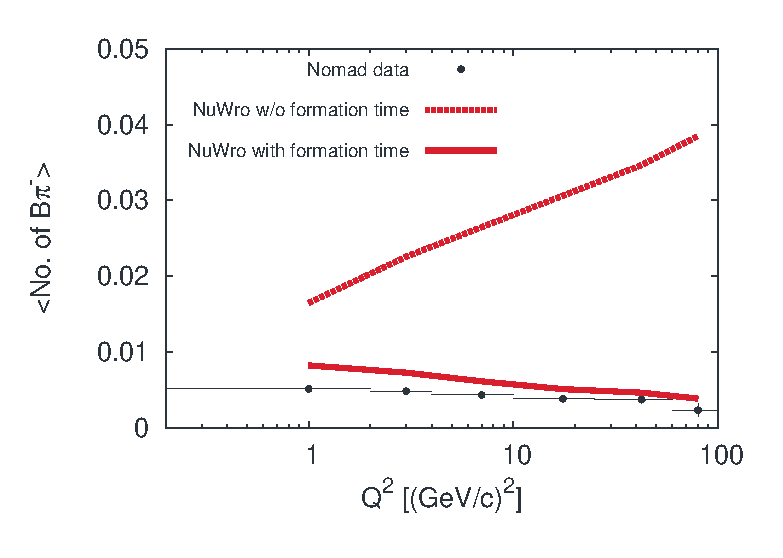
\includegraphics[width=0.5\slidewidth]{img/nomad.eps}}
 
\end{slide}

%%%%% NC PI0 %%%%%

\begin{slide}[toc=NC $\pi$]{Comparison with data for NC $\pi^0$ production}

  \rput(12, 4.25){% ncpi0 signal
\begin{pspicture}
  
  \pscircle[linestyle = none, fillstyle = solid, fillcolor = pdcolor1](0,0){1}

  \pscircle[linestyle = none, fillstyle = solid, fillcolor = pdcolor4](-2.5,0){0.2}
  \psline[linewidth = 0.05, linecolor = pdcolor4]{->}(-2.1,0)(-1.2,0)
  \rput[c](-1.75,0.25){\color{pdcolor4}\small $\left<E_\nu\right>$}
  \rput[c](-1.75,-0.24){\color{pdcolor4}\small $\sim 1$~GeV}
  \psline[linewidth = 0.05, linecolor = pdcolor1]{->}(1.2,0)(1.6,0)
  
  \rput[l](2,0.75){\color{pdcolor1} 0$\mu$}
  \rput[l](2,0){\color{pdcolor1} 0$\pi^\pm$}
  \rput[l](2,-0.75){\color{pdcolor1} 1$\pi^0$}
  
\end{pspicture}
}

  \begin{itemize}
   
   \item The cross section \\ for $\pi^0$ production \\ through neutral current \\ is measured by \\ K2K [1], MiniBooNE [2] and SciBooNE [3] experiments.
   
   \item The signal is defined as: no charged leptons nor charged pions and one neutral pion (or at least one for ScibooNE) in the final state.
   
   \item The result depends on primary vertex and FSI, as $\pi$ can be:
   
    \begin{itemize}
    
      \item produced in primary vertex;
      \item produced in FSI;
      \item affected by charge exchange;
      \item absorbed.
    
    \end{itemize}
    
  \end{itemize}

  \rput[l](6.25,2){\color{pdcolor3}\footnotesize [1] Phys. Lett. B619 (2005) 255}
  \rput[l](6.25,1.5){\color{pdcolor3}\footnotesize [2] Phys. Rev. D81 (2010) 013005}
  \rput[l](6.25,1){\color{pdcolor3}\footnotesize [3] Phys. Rev. D81 (2009) 033004}
  
\end{slide}

\begin{wideslide}[toc=]{Comparison with data for NC $\pi^0$ production}
 
  \hspace{20pt}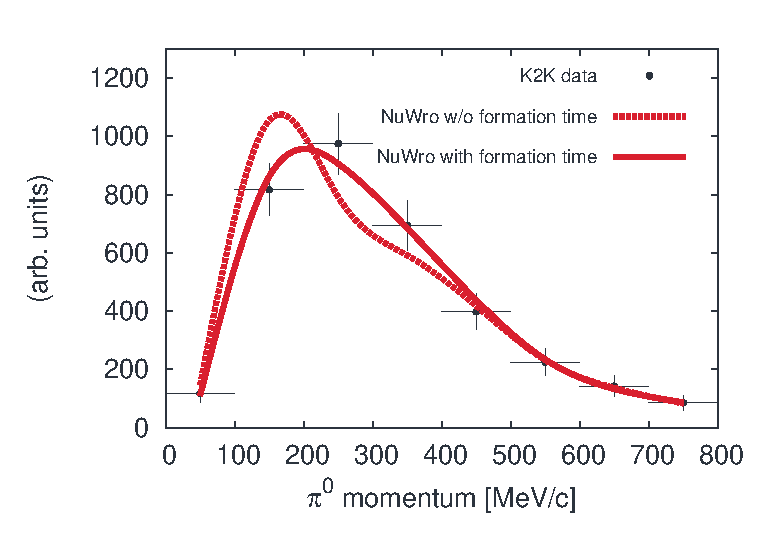
\includegraphics[width = 0.425\slidewidth]{img/k2k.eps}
  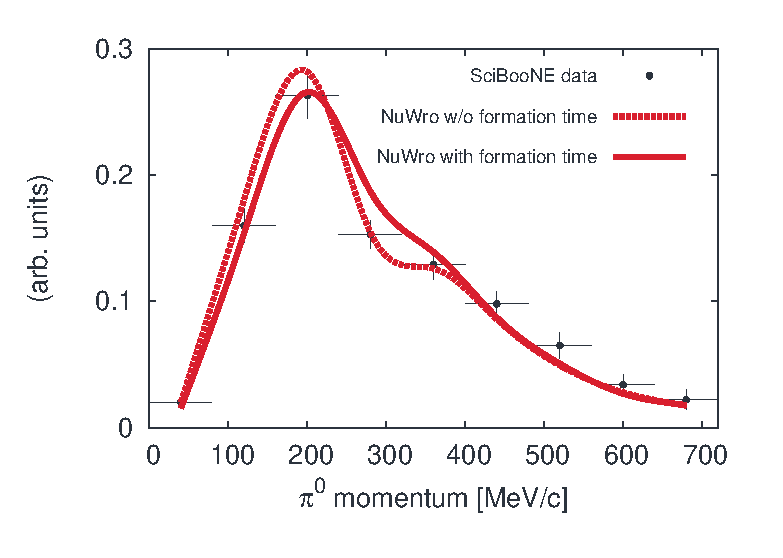
\includegraphics[width = 0.425\slidewidth]{img/sb.eps}\\
  \hspace{20pt}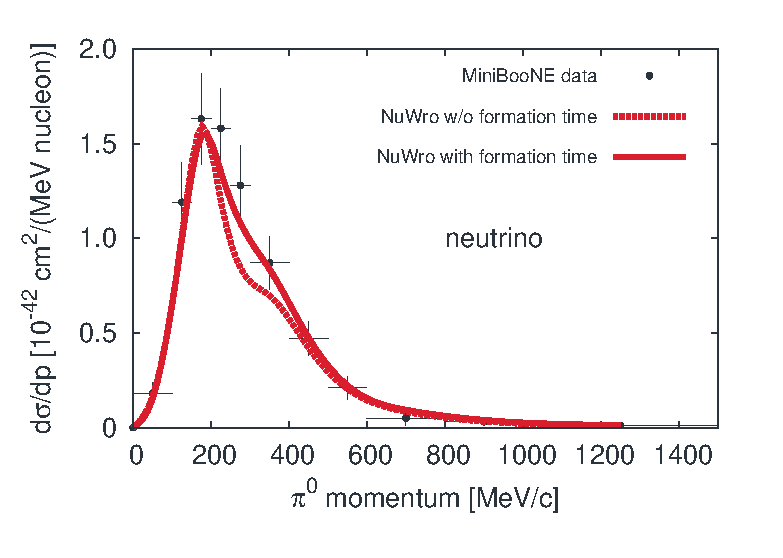
\includegraphics[width = 0.425\slidewidth]{img/mb.eps}
  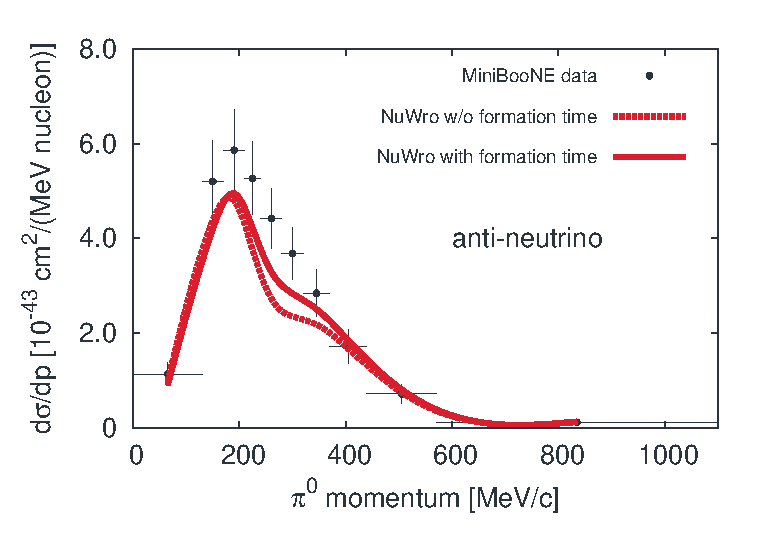
\includegraphics[width = 0.425\slidewidth]{img/mba.eps}
 
\end{wideslide}

%%%%% INTERACTIONS SUMMARY %%%%%

\begin{wideslide}[toc=Summary]{Neutrino-nucleus interactions}
\null\vfill

  \sep

  For all channels (but coherent) neutrino interactions are factorized in the following way
  
  \sep\sep\sep
  
  \centering\begin{tikzpicture}
 
  \draw [rounded corners] (0,0) -- (2,0) -- (2,2) -- (0,2) -- cycle;
  \draw [rounded corners] (2.5,0) -- (4.5,0) -- (4.5,2) -- (2.5,2) -- cycle;
  \draw [rounded corners] (5,0) -- (7,0) -- (7,2) -- (5,2) -- cycle;
  \draw [rounded corners] (7.5,0) -- (9.5,0) -- (9.5,2) -- (7.5,2) -- cycle;
  \draw [rounded corners] (10,0) -- (12,0) -- (12,2) -- (10,2) -- cycle;
  
  \draw (1,1) circle (0.75cm);
  
  \draw [filled=pdcolor4, draw=none] (1.1, 1.2) circle (0.1cm);    
  \draw [filled=pdcolor5, draw=none] (1.4, 1.3) circle (0.1cm);    
  \draw [filled=pdcolor4, draw=none] (1.5, 0.9) circle (0.1cm);    
  \draw [filled=pdcolor5, draw=none] (1.3, 0.6) circle (0.1cm);    
  \draw [filled=pdcolor4, draw=none] (0.8, 1.4) circle (0.1cm);    
  \draw [filled=pdcolor5, draw=none] (0.5, 1.0) circle (0.1cm);    
  \draw [filled=pdcolor4, draw=none] (0.8, 0.7) circle (0.1cm);
  
  \draw (3,0.5) -- (3.5,1) -- (3,1.5);
  \draw [curl] (3.5,1) -- (4.1,1);
  \draw [filled=pdcolor1, draw=none] (3,0.5) circle (0.1cm);
  \draw [filled=pdcolor1, draw=none] (3,1.5) circle (0.1cm);
  \draw [filled=pdcolor4, draw=none] (4.1,1) circle (0.1cm);
  
  \node at (6,1) {\scalebox{0.2}{\begin{tikzpicture}
  
  \node (center) {};
  
  \node [circle, filled={pdcolor4}, minimum width = 1cm, below=of center, xshift = 3cm, yshift = 0cm] {}; 
  \node [circle, filled={pdcolor5}, minimum width = 1cm, below=of center, xshift = 6cm, yshift = 1cm] {}; 
  \node [circle, filled={pdcolor6}, minimum width = 1cm, below=of center, xshift = 2cm, yshift = 2cm] {}; 
  \node [circle, filled={pdcolor7}, minimum width = 1cm, below=of center, xshift = 0cm, yshift = 3cm] {}; 
  \node [circle, filled={pdcolor4}, minimum width = 1cm, below=of center, xshift = 1cm, yshift = 4cm] {}; 
  \node [circle, filled={pdcolor5}, minimum width = 1cm, below=of center, xshift = 4cm, yshift = 3.5cm] {}; 
  \node [circle, filled={pdcolor6}, minimum width = 1cm, below=of center, xshift = 2.5cm, yshift = 3.5cm] {}; 
  \node [circle, filled={pdcolor7}, minimum width = 1cm, below=of center, xshift = 4.25cm, yshift = 1.5cm] {}; 
 
\end{tikzpicture}
}};
 
  \foreach \x in {1,...,10}
  {
    \pgfmathsetmacro{\r}{\x / 100}
    \pgfmathsetmacro{\o}{\x / 10}
    \draw [filled=pdcolor1, draw=none, fill opacity = \o] (8 + \o, 1) circle (\r cm);  
    \draw [filled=pdcolor4, draw=none, fill opacity = \o] (8 + \o, 1 + \o / 2) circle (\r cm);  
    \draw [filled=pdcolor6, draw=none, fill opacity = \o] (8 + \o, 1 - \o / 2) circle (\r cm);  
  }
  
  \node [below] at (1.0, 0) {IA};
  \node [below] at (3.5, 0) {$\nu N$};
  \node [below] at (6.0, 0) {hadronization};
  \node [below] at (8.5, 0) {formation time};
  \node [below] at (11., 0) {FSI};
  
  \node at (11,1) {\scalebox{0.2}{\tikzset{
p/.style = {ultra thick, color = pdcolor1, >=latex, ->},
n/.style = {ultra thick, color = pdcolor4, >=latex, ->},
pi/.style = {ultra thick, color = pdcolor5, >=latex, ->},
pip/.style = {ultra thick, color = pdcolor6, >=latex, ->},
pim/.style = {ultra thick, color = pdcolor7, >=latex, ->},
}

\begin{tikzpicture}
    
    \draw[n] (-2,0) -- node[left] {$n$} (-1,1.5);
    \draw[p] (-1,1.5) -- (-1, 3.5) node[left] {$p$};
    \draw[n] (-1,1.5) -- node[above] {$n$} (0,1.5);
    \draw[p] (0,1.5) -- (2.5,3) node[above] {$p$};
    \draw[pim] (0, 1.5) -- node[above] {$\pi^-$} (1.5, 0.5);
    \draw[pim] (1.5, 0.5) -- (3.75, 0.25) node[above] {$\pi^-$};
    \draw[n] (1.5, 0.5) -- node[right] {$n$} (1.75, -0.5);
    
    \draw[pip] (-2,0) -- node[above] {$\pi^+$} (-0.5,0);
    \draw[p] (-0.5,0) -- node[above] {$p$} (0, 0.5);
    \draw[pi] (-0.5,0) -- node[above] {$\pi^0$} (1,-1);
    \draw[n] (1,-1) -- (3.5,-1.5) node[above] {$n$};
    \draw[p] (1,-1) -- (2.75, -2.75) node [right] {$p$};
    
    \draw[pi] (-2,0) -- node[left] {$\pi^0$} (-1,-1.5);
    \draw[pim] (-1,-1.5) -- (-1.5, -3.5) node[right] {$\pi^-$};
    \draw[pip] (-1,-1.5) -- (0, -3.5) node[right] {$\pi^+$};
    \draw[n] (-1,-1.5) -- node[above] {$n$} (0, -2);
    \draw[n] (0,-2) -- node[above] {$n$} (1, -1.5);
    \draw[p] (0,-2) -- node[below] {$p$} (1, -2.5);
    
    \draw[ultra thick, color = pdcolor1] (0,0) circle (3);
    
    \draw[ultra thick, color = pdcolor1, >=latex, ->] (-4, 0) -- (-2,0);

\end{tikzpicture}
}};
 
\end{tikzpicture}

  
  \sep\sep
  
  \begin{itemize}
   \item Is the physics really factorized this way?
   \item This factorization is common for all generators
   \item However, some pieces are done in different way
  \end{itemize}
  
\vfill\null
\end{wideslide}
